% Options for packages loaded elsewhere
\PassOptionsToPackage{unicode}{hyperref}
\PassOptionsToPackage{hyphens}{url}
\PassOptionsToPackage{dvipsnames,svgnames,x11names}{xcolor}
%
\documentclass[
]{book}
\usepackage{amsmath,amssymb}
\usepackage{iftex}
\ifPDFTeX
  \usepackage[T1]{fontenc}
  \usepackage[utf8]{inputenc}
  \usepackage{textcomp} % provide euro and other symbols
\else % if luatex or xetex
  \usepackage{unicode-math} % this also loads fontspec
  \defaultfontfeatures{Scale=MatchLowercase}
  \defaultfontfeatures[\rmfamily]{Ligatures=TeX,Scale=1}
\fi
\usepackage{lmodern}
\ifPDFTeX\else
  % xetex/luatex font selection
\fi
% Use upquote if available, for straight quotes in verbatim environments
\IfFileExists{upquote.sty}{\usepackage{upquote}}{}
\IfFileExists{microtype.sty}{% use microtype if available
  \usepackage[]{microtype}
  \UseMicrotypeSet[protrusion]{basicmath} % disable protrusion for tt fonts
}{}
\makeatletter
\@ifundefined{KOMAClassName}{% if non-KOMA class
  \IfFileExists{parskip.sty}{%
    \usepackage{parskip}
  }{% else
    \setlength{\parindent}{0pt}
    \setlength{\parskip}{6pt plus 2pt minus 1pt}}
}{% if KOMA class
  \KOMAoptions{parskip=half}}
\makeatother
\usepackage{xcolor}
\usepackage[b5paper,tmargin=1.5cm,bmargin=1.5cm,lmargin=1.0cm,rmargin=1.0cm]{geometry}
\usepackage{color}
\usepackage{fancyvrb}
\newcommand{\VerbBar}{|}
\newcommand{\VERB}{\Verb[commandchars=\\\{\}]}
\DefineVerbatimEnvironment{Highlighting}{Verbatim}{commandchars=\\\{\}}
% Add ',fontsize=\small' for more characters per line
\usepackage{framed}
\definecolor{shadecolor}{RGB}{248,248,248}
\newenvironment{Shaded}{\begin{snugshade}}{\end{snugshade}}
\newcommand{\AlertTok}[1]{\textcolor[rgb]{0.94,0.16,0.16}{#1}}
\newcommand{\AnnotationTok}[1]{\textcolor[rgb]{0.56,0.35,0.01}{\textbf{\textit{#1}}}}
\newcommand{\AttributeTok}[1]{\textcolor[rgb]{0.13,0.29,0.53}{#1}}
\newcommand{\BaseNTok}[1]{\textcolor[rgb]{0.00,0.00,0.81}{#1}}
\newcommand{\BuiltInTok}[1]{#1}
\newcommand{\CharTok}[1]{\textcolor[rgb]{0.31,0.60,0.02}{#1}}
\newcommand{\CommentTok}[1]{\textcolor[rgb]{0.56,0.35,0.01}{\textit{#1}}}
\newcommand{\CommentVarTok}[1]{\textcolor[rgb]{0.56,0.35,0.01}{\textbf{\textit{#1}}}}
\newcommand{\ConstantTok}[1]{\textcolor[rgb]{0.56,0.35,0.01}{#1}}
\newcommand{\ControlFlowTok}[1]{\textcolor[rgb]{0.13,0.29,0.53}{\textbf{#1}}}
\newcommand{\DataTypeTok}[1]{\textcolor[rgb]{0.13,0.29,0.53}{#1}}
\newcommand{\DecValTok}[1]{\textcolor[rgb]{0.00,0.00,0.81}{#1}}
\newcommand{\DocumentationTok}[1]{\textcolor[rgb]{0.56,0.35,0.01}{\textbf{\textit{#1}}}}
\newcommand{\ErrorTok}[1]{\textcolor[rgb]{0.64,0.00,0.00}{\textbf{#1}}}
\newcommand{\ExtensionTok}[1]{#1}
\newcommand{\FloatTok}[1]{\textcolor[rgb]{0.00,0.00,0.81}{#1}}
\newcommand{\FunctionTok}[1]{\textcolor[rgb]{0.13,0.29,0.53}{\textbf{#1}}}
\newcommand{\ImportTok}[1]{#1}
\newcommand{\InformationTok}[1]{\textcolor[rgb]{0.56,0.35,0.01}{\textbf{\textit{#1}}}}
\newcommand{\KeywordTok}[1]{\textcolor[rgb]{0.13,0.29,0.53}{\textbf{#1}}}
\newcommand{\NormalTok}[1]{#1}
\newcommand{\OperatorTok}[1]{\textcolor[rgb]{0.81,0.36,0.00}{\textbf{#1}}}
\newcommand{\OtherTok}[1]{\textcolor[rgb]{0.56,0.35,0.01}{#1}}
\newcommand{\PreprocessorTok}[1]{\textcolor[rgb]{0.56,0.35,0.01}{\textit{#1}}}
\newcommand{\RegionMarkerTok}[1]{#1}
\newcommand{\SpecialCharTok}[1]{\textcolor[rgb]{0.81,0.36,0.00}{\textbf{#1}}}
\newcommand{\SpecialStringTok}[1]{\textcolor[rgb]{0.31,0.60,0.02}{#1}}
\newcommand{\StringTok}[1]{\textcolor[rgb]{0.31,0.60,0.02}{#1}}
\newcommand{\VariableTok}[1]{\textcolor[rgb]{0.00,0.00,0.00}{#1}}
\newcommand{\VerbatimStringTok}[1]{\textcolor[rgb]{0.31,0.60,0.02}{#1}}
\newcommand{\WarningTok}[1]{\textcolor[rgb]{0.56,0.35,0.01}{\textbf{\textit{#1}}}}
\usepackage{longtable,booktabs,array}
\usepackage{calc} % for calculating minipage widths
% Correct order of tables after \paragraph or \subparagraph
\usepackage{etoolbox}
\makeatletter
\patchcmd\longtable{\par}{\if@noskipsec\mbox{}\fi\par}{}{}
\makeatother
% Allow footnotes in longtable head/foot
\IfFileExists{footnotehyper.sty}{\usepackage{footnotehyper}}{\usepackage{footnote}}
\makesavenoteenv{longtable}
\usepackage{graphicx}
\makeatletter
\def\maxwidth{\ifdim\Gin@nat@width>\linewidth\linewidth\else\Gin@nat@width\fi}
\def\maxheight{\ifdim\Gin@nat@height>\textheight\textheight\else\Gin@nat@height\fi}
\makeatother
% Scale images if necessary, so that they will not overflow the page
% margins by default, and it is still possible to overwrite the defaults
% using explicit options in \includegraphics[width, height, ...]{}
\setkeys{Gin}{width=\maxwidth,height=\maxheight,keepaspectratio}
% Set default figure placement to htbp
\makeatletter
\def\fps@figure{htbp}
\makeatother
\setlength{\emergencystretch}{3em} % prevent overfull lines
\providecommand{\tightlist}{%
  \setlength{\itemsep}{0pt}\setlength{\parskip}{0pt}}
\setcounter{secnumdepth}{5}
% definitions for citeproc citations
\NewDocumentCommand\citeproctext{}{}
\NewDocumentCommand\citeproc{mm}{%
  \begingroup\def\citeproctext{#2}\cite{#1}\endgroup}
\makeatletter
 % allow citations to break across lines
 \let\@cite@ofmt\@firstofone
 % avoid brackets around text for \cite:
 \def\@biblabel#1{}
 \def\@cite#1#2{{#1\if@tempswa , #2\fi}}
\makeatother
\newlength{\cslhangindent}
\setlength{\cslhangindent}{1.5em}
\newlength{\csllabelwidth}
\setlength{\csllabelwidth}{3em}
\newenvironment{CSLReferences}[2] % #1 hanging-indent, #2 entry-spacing
 {\begin{list}{}{%
  \setlength{\itemindent}{0pt}
  \setlength{\leftmargin}{0pt}
  \setlength{\parsep}{0pt}
  % turn on hanging indent if param 1 is 1
  \ifodd #1
   \setlength{\leftmargin}{\cslhangindent}
   \setlength{\itemindent}{-1\cslhangindent}
  \fi
  % set entry spacing
  \setlength{\itemsep}{#2\baselineskip}}}
 {\end{list}}
\usepackage{calc}
\newcommand{\CSLBlock}[1]{\hfill\break\parbox[t]{\linewidth}{\strut\ignorespaces#1\strut}}
\newcommand{\CSLLeftMargin}[1]{\parbox[t]{\csllabelwidth}{\strut#1\strut}}
\newcommand{\CSLRightInline}[1]{\parbox[t]{\linewidth - \csllabelwidth}{\strut#1\strut}}
\newcommand{\CSLIndent}[1]{\hspace{\cslhangindent}#1}
\usepackage{booktabs}
% \usepackage{fontspec} %這個可能原本文檔就已經有了,放入時候check一下
% \usepackage{CJKutf8}
% \usepackage[UTF8]{inputenc}
\usepackage{CJK}
% \usepackage{xeCJK}

%英文字體調整(有時候交中文文件可能有規定對應的英文字體)
% \setmainfont{Times New Roman}
% \setmainfont{Noto Sans}

%中文字體main跟mono都需要哦,最後面的SC是簡體中文,也可以改成TC,不過SC的破字會比較少
% \setCJKmainfont{NotoSansTC-Regular.otf}
% \setCJKmonofont{NotoSansTC-Regular.otf}

% \usepackage{bm}
\usepackage{amsmath,amssymb}
% \usepackage[pagebackref=true]{hyperref}
% \usepackage[backref]{hyperref}
\usepackage[]{hyperref}
\usepackage[hyperpageref]{backref}
\hypersetup{
    colorlinks=true,
    linkcolor=blue,
    filecolor=magenta,      
    urlcolor=cyan
}

% \usepackage{fdsymbol} % vector over accent, but will use mathptmx
%% replace the rather ugly mathptmx \sum operator with the equivalent Computer Modern one
% \let\sum\relax
% \DeclareSymbolFont{CMlargesymbols}{OMX}{cmex}{m}{n}
% \DeclareMathSymbol{\sum}{\mathop}{CMlargesymbols}{"50}

\usepackage{cancel} % demo usepackage in PDF and require in HTML

% to wrap the text inside the margins of the PDF document when using code chunks in bookdown
\usepackage{fvextra}
\DefineVerbatimEnvironment{Highlighting}{Verbatim}{breaklines,commandchars=\\\{\}}

% \usepackage[backend=bibtex]{biblatex}
% \usepackage[backend=biber]{biblatex}
% \usepackage[]{biblatex}
% \DeclarePrintbibliographyDefaults{heading=bibintoc}

% \let\oldpb\printbibliography
% \renewcommand{\printbibliography}{\oldpb[heading=bibintoc]}

% https://bookdown.org/yihui/rmarkdown-cookbook/figure-placement.html % to use fig.pos = "H" for multi-column fig.cap
\usepackage{float}

% https://tex.stackexchange.com/questions/128485/how-to-make-a-caption-via-captionof-and-extra-margins-adhere-to-minipage-marg
% \usepackage[labelfont=sf,hypcap=false,format=hang,width=0.8\columnwidth]{caption}

% SVG
\usepackage{svg}

% TikZ
\usepackage{tikz}
\usepackage{tikz-3dplot}
\usepackage{pgfplots}
\pgfplotsset{compat=1.15}
% animation
\usepackage[autoplay]{animate}

% xcolor colorbox
% https://www.overleaf.com/learn/latex/Using_colors_in_LaTeX
\usepackage[dvipsnames]{xcolor}
% \usepackage[svgnames]{xcolor}
% \usepackage[x11names]{xcolor}

\usepackage{mathrsfs}
\usetikzlibrary{arrows}
% \pagestyle{empty}
% \newcommand{\degre}{\ensuremath{^\circ}}

\usepackage[all]{xy}

% LaTeX Error: Too deeply nested
% https://stackoverflow.com/questions/57945414/too-deeply-nested-at-just-fourth-nesting-level-using-pandoc-with-markdown
\usepackage{enumitem}
\setlistdepth{20}
\renewlist{itemize}{itemize}{20}
\renewlist{enumerate}{enumerate}{20}
\setlist[itemize]{label=$\cdot$}
\setlist[itemize,1]{label=\textbullet}
\setlist[itemize,2]{label=--}
\setlist[itemize,3]{label=*}

% multicolumn
% https://bookdown.org/yihui/rmarkdown-cookbook/multi-column.html
\newenvironment{cols}[1][]{}{}

\newenvironment{col}[1]{\begin{minipage}{#1}\ignorespaces}{%
\end{minipage}
\ifhmode\unskip\fi
\aftergroup\useignorespacesandallpars}

\def\useignorespacesandallpars#1\ignorespaces\fi{%
#1\fi\ignorespacesandallpars}

\makeatletter
\def\ignorespacesandallpars{%
  \@ifnextchar\par
    {\expandafter\ignorespacesandallpars\@gobble}%
    {}%
}
\makeatother
\usepackage{float}
\ifLuaTeX
  \usepackage{selnolig}  % disable illegal ligatures
\fi
\usepackage{bookmark}
\IfFileExists{xurl.sty}{\usepackage{xurl}}{} % add URL line breaks if available
\urlstyle{same}
\hypersetup{
  pdftitle={math},
  pdfauthor={Joey Yu Hsu},
  colorlinks=true,
  linkcolor={Maroon},
  filecolor={Maroon},
  citecolor={Blue},
  urlcolor={Blue},
  pdfcreator={LaTeX via pandoc}}

\title{math}
\author{Joey Yu Hsu}
\date{2024-03-29}

\usepackage{amsthm}
\newtheorem{theorem}{Theorem}[chapter]
\newtheorem{lemma}{Lemma}[chapter]
\newtheorem{corollary}{Corollary}[chapter]
\newtheorem{proposition}{Proposition}[chapter]
\newtheorem{conjecture}{Conjecture}[chapter]
\theoremstyle{definition}
\newtheorem{definition}{Definition}[chapter]
\theoremstyle{definition}
\newtheorem{example}{Example}[chapter]
\theoremstyle{definition}
\newtheorem{exercise}{Exercise}[chapter]
\theoremstyle{definition}
\newtheorem{hypothesis}{Hypothesis}[chapter]
\theoremstyle{remark}
\newtheorem*{remark}{Remark}
\newtheorem*{solution}{Solution}
\begin{document}
\maketitle

{
\hypersetup{linkcolor=}
\setcounter{tocdepth}{4}
\tableofcontents
}
\chapter*{index}\label{index}
\addcontentsline{toc}{chapter}{index}

math on bookdown started on 2024/01/28

\part{by descipline}\label{part-by-descipline}

\chapter{mathematics}\label{mathematics}

\section{tool}\label{tool}

\begin{itemize}
\tightlist
\item
  formula typesetting

  \begin{itemize}
  \tightlist
  \item
    TeX

    \begin{itemize}
    \tightlist
    \item
      LaTeX

      \begin{itemize}
      \tightlist
      \item
        pdfLaTeX
      \item
        XeLaTeX
      \item
        editor/tool:

        \begin{itemize}
        \tightlist
        \item
          LyX
        \item
          OverLeaf
        \item
          MathPix Snip
        \item
          Micro\$oft Office Word

          \begin{itemize}
          \tightlist
          \item
            WordTeX \url{https://tomwildenhain.com/wordtex/}

            \begin{itemize}
            \tightlist
            \item
              Pandoc dependent
            \end{itemize}
          \item
            \url{https://superuser.com/questions/1114697/select-a-different-math-font-in-microsoft-word}
          \item
            \url{https://www.youtube.com/watch?v=jlX_pThh7z8}
          \end{itemize}
        \item
          Micro\$oft Office PowerPoint

          \begin{itemize}
          \tightlist
          \item
            IguanaTeX \url{https://www.jonathanleroux.org/software/iguanatex/}
          \end{itemize}
        \end{itemize}
      \end{itemize}
    \end{itemize}
  \item
    MathML
  \item
    MathJax: JavaScript
  \end{itemize}
\item
  \hyperref[plot]{plot}\textsuperscript{{[}\ref{plot}{]}}
\item
  symbolic computing

  \begin{itemize}
  \tightlist
  \item
    Maple: by MapleSoft
  \item
    Mathematica: by Wolfram
  \end{itemize}
\item
  numeric computing

  \begin{itemize}
  \tightlist
  \item
    MatLab: by MathWorks
  \end{itemize}
\end{itemize}

\hyperref[equivalence-relation]{equivalence relation}\textsuperscript{{[}\ref{equivalence-relation}{]}}

\hyperref[equivalence-class]{equivalence class}\textsuperscript{{[}\ref{equivalence-class}{]}}

\hyperref[partition]{partition}\textsuperscript{{[}\ref{partition}{]}}

\section{discipline}\label{discipline}

\chapter{physics}\label{physics}

\section{discipline}\label{discipline-1}

\begin{itemize}
\tightlist
\item
  relativity

  \begin{itemize}
  \tightlist
  \item
    special relativity

    \begin{itemize}
    \tightlist
    \item
      \hyperref[lorentz-transformation]{Lorentz transformation}\textsuperscript{{[}\ref{lorentz-transformation}{]}}
    \end{itemize}
  \item
    general relativity
  \end{itemize}
\item
  analytic mechanics

  \begin{itemize}
  \tightlist
  \item
    Lagrangian mechanics
  \item
    Hamiltonian mechanics
  \end{itemize}
\item
  electromagnetism
\item
  quantum mechanics
\item
  field theory
\end{itemize}

\chapter{plot}\label{plot}

\begin{itemize}
\tightlist
\item
  LaTeX

  \begin{itemize}
  \tightlist
  \item
    \hyperref[tikz]{TikZ}\textsuperscript{{[}\ref{tikz}{]}}

    \begin{itemize}
    \tightlist
    \item
      \url{https://tikz.dev/}
    \item
      TikZ-3Dplot
    \item
      \hyperref[pgfplots]{PGFplots}\textsuperscript{{[}\ref{pgfplots}{]}}

      \begin{itemize}
      \tightlist
      \item
        \url{https://tikz.dev/pgfplots/}
      \item
        \url{https://pgfplots.sourceforge.net/gallery.html}
      \item
        \url{https://pgfplots.net/}
      \end{itemize}
    \item
      editor / export

      \begin{itemize}
      \tightlist
      \item
        \url{https://zhuanlan.zhihu.com/p/660371706}
      \item
        offline

        \begin{itemize}
        \tightlist
        \item
          \href{http://www.tikzedt.org/}{TikzEdt}: WYSIWYG and live preview
        \item
          \href{https://tikzit.github.io/}{TikZiT}
        \end{itemize}
      \item
        online

        \begin{itemize}
        \tightlist
        \item
          OverLeaf
        \item
          MathCha
        \item
          GeoGebra Classic
        \end{itemize}
      \item
        Python

        \begin{itemize}
        \tightlist
        \item
          TikZplotLib / tikzplotlib\textsuperscript{{[}\ref{tikzplotlib}{]}}

          \begin{itemize}
          \tightlist
          \item
            matplotlib export to TikZ .tex
          \item
            \href{https://pypi.org/project/tikzplotlib/}{PyPI}
          \item
            \href{https://github.com/nschloe/tikzplotlib}{GitHub}
          \end{itemize}
        \end{itemize}
      \item
        R

        \begin{itemize}
        \tightlist
        \item
          TikZDevice / tikzDevice

          \begin{itemize}
          \tightlist
          \item
            r chunk \texttt{engine=\textquotesingle{}tikz\textquotesingle{}} knitr \texttt{out.width=if\ (knitr:::is\_html\_output())\ \textquotesingle{}100\%\textquotesingle{}}
          \item
            \href{https://cran.r-project.org/web/packages/tikzDevice/index.html}{CRAN}

            \begin{itemize}
            \tightlist
            \item
              \href{https://cran.r-project.org/web/packages/tikzDevice/tikzDevice.pdf}{reference manual}
            \item
              vignette: \href{https://cran.r-project.org/web/packages/tikzDevice/vignettes/tikzDevice.pdf}{TikZDevice - LaTeX Graphics for R}
            \end{itemize}
          \item
            \href{https://github.com/daqana/tikzDevice}{GitHub}
          \end{itemize}
        \end{itemize}
      \end{itemize}
    \item
      \href{https://tex.stackexchange.com/questions/42611/list-of-available-tikz-libraries-with-a-short-introduction}{TikZ library}
    \end{itemize}
  \item
    xypic = \hyperref[xy-pic]{xy-pic}\textsuperscript{{[}\ref{xy-pic}{]}}
  \end{itemize}
\item
  \href{https://www.overleaf.com/}{OverLeaf}
\item
  \href{https://www.mathcha.io/}{MathCha}
\item
  \href{https://www.geogebra.org/}{GeoGebra}

  \begin{itemize}
  \tightlist
  \item
    \href{https://www.geogebra.org/classic}{GeoGebra Classic}: to export TikZ
  \item
    \href{https://www.geogebra.org/calculator}{GeoGebra Calculator Suite}
  \end{itemize}
\item
  Python

  \begin{itemize}
  \tightlist
  \item
    MatPlotLib / matplotlib\textsuperscript{{[}\ref{matplotlib}{]}}
  \item
    \hyperref[seaborn]{Seaborn} / seaborn\textsuperscript{{[}\ref{seaborn}{]}}
  \item
    Plotly
  \item
    Manim
  \end{itemize}
\item
  R

  \begin{itemize}
  \tightlist
  \item
    \href{https://bookdown.org/xiangyun/msg/}{Modern Statistical Graphics}
  \item
    \hyperref[ggplot2]{ggplot2}\textsuperscript{{[}\ref{ggplot2}{]}}

    \begin{itemize}
    \tightlist
    \item
      Modern Statistical Graphics \href{https://bookdown.org/xiangyun/msg/system.html\#sec:ggplot2}{section 5.1}
    \end{itemize}
  \item
    GraphViz \texttt{.gv}
  \item
    Mermaid \texttt{.mmd}

    \begin{itemize}
    \tightlist
    \item
      \href{https://mermaid.js.org/intro/}{about}
    \item
      JavaScript based diagramming and charting tool that renders Markdown-inspired text definitions to create and modify diagrams dynamically
    \end{itemize}
  \item
    Shiny

    \begin{itemize}
    \tightlist
    \item
      R Markdown Guide \href{https://cosname.github.io/rmarkdown-guide/rmarkdown-interaction.html\#rmarkdown-shiny}{section 5.1}
    \end{itemize}
  \item
    tool

    \begin{itemize}
    \tightlist
    \item
      Jamovi
    \end{itemize}
  \end{itemize}
\end{itemize}

neural network plot/draw
\url{https://github.com/ashishpatel26/Tools-to-Design-or-Visualize-Architecture-of-Neural-Network}

\chapter{programming language}\label{programming-language}

\section{discipline}\label{discipline-2}

\begin{itemize}
\tightlist
\item
  \hyperref[python]{Python}\textsuperscript{{[}\ref{python}{]}}
\item
  JavaScript
\item
  SQL = structured query language
\item
  \hyperref[r]{R}\textsuperscript{{[}\ref{r}{]}}

  \begin{itemize}
  \tightlist
  \item
    RMarkdown

    \begin{itemize}
    \tightlist
    \item
      Bookdown
    \end{itemize}
  \item
    knitr: engine

    \begin{itemize}
    \tightlist
    \item
      \hyperref[tikz]{TikZ}\textsuperscript{{[}\ref{tikz}{]}}
    \end{itemize}
  \item
    reticulate: Python
  \item
    Jamovi
  \end{itemize}
\item
  C\#

  \begin{itemize}
  \tightlist
  \item
    web

    \begin{itemize}
    \tightlist
    \item
      MVC
    \item
      .NET
    \end{itemize}
  \item
    desktop

    \begin{itemize}
    \tightlist
    \item
      UWP = Universal Windows Platform
    \item
      WPF = Windows Presentation Foundation
    \item
      WinForms = Windows Forms
    \end{itemize}
  \item
    3D/game

    \begin{itemize}
    \tightlist
    \item
      Unity
    \end{itemize}
  \end{itemize}
\end{itemize}

\section{learning map}\label{learning-map-2}

\begin{itemize}
\tightlist
\item
  \href{https://www.w3schools.com/}{W3School}
\item
  \href{https://www.sololearn.com/}{SoloLearn}
\item
  \href{https://www.codecademy.com/}{Codecademy}
\end{itemize}

\chapter{machine learning}\label{machine-learning}

\part{by date}\label{part-by-date}

\chapter{A Minimal Book Example}\label{a-minimal-book-example}

\section{About}\label{about}

This is a \emph{sample} book written in \textbf{Markdown}. You can use anything that Pandoc's Markdown supports; for example, a math equation \(a^2 + b^2 = c^2\).

\subsection{Usage}\label{usage}

Each \textbf{bookdown} chapter is an .Rmd file, and each .Rmd file can contain one (and only one) chapter. A chapter \emph{must} start with a first-level heading: \texttt{\#\ A\ good\ chapter}, and can contain one (and only one) first-level heading.

Use second-level and higher headings within chapters like: \texttt{\#\#\ A\ short\ section} or \texttt{\#\#\#\ An\ even\ shorter\ section}.

The \texttt{index.Rmd} file is required, and is also your first book chapter. It will be the homepage when you render the book.

\subsection{Render book}\label{render-book}

You can render the HTML version of this example book without changing anything:

\begin{enumerate}
\def\labelenumi{\arabic{enumi}.}
\item
  Find the \textbf{Build} pane in the RStudio IDE, and
\item
  Click on \textbf{Build Book}, then select your output format, or select ``All formats'' if you'd like to use multiple formats from the same book source files.
\end{enumerate}

Or build the book from the R console:

\begin{Shaded}
\begin{Highlighting}[]
\NormalTok{bookdown}\SpecialCharTok{::}\FunctionTok{render\_book}\NormalTok{()}
\end{Highlighting}
\end{Shaded}

To render this example to PDF as a \texttt{bookdown::pdf\_book}, you'll need to install XeLaTeX. You are recommended to install TinyTeX (which includes XeLaTeX): \url{https://yihui.org/tinytex/}.

\subsection{Preview book}\label{preview-book}

As you work, you may start a local server to live preview this HTML book. This preview will update as you edit the book when you save individual .Rmd files. You can start the server in a work session by using the RStudio add-in ``Preview book'', or from the R console:

\begin{Shaded}
\begin{Highlighting}[]
\NormalTok{bookdown}\SpecialCharTok{::}\FunctionTok{serve\_book}\NormalTok{()}
\end{Highlighting}
\end{Shaded}

\section{Hello bookdown}\label{hello-bookdown}

All chapters start with a first-level heading followed by your chapter title, like the line above. There should be only one first-level heading (\texttt{\#}) per .Rmd file.

\subsection{A section}\label{a-section}

All chapter sections start with a second-level (\texttt{\#\#}) or higher heading followed by your section title, like the sections above and below here. You can have as many as you want within a chapter.

\subsubsection*{An unnumbered section}\label{an-unnumbered-section}
\addcontentsline{toc}{subsubsection}{An unnumbered section}

Chapters and sections are numbered by default. To un-number a heading, add a \texttt{\{.unnumbered\}} or the shorter \texttt{\{-\}} at the end of the heading, like in this section.

\section{Cross-references}\label{cross}

Cross-references make it easier for your readers to find and link to elements in your book.

\subsection{Chapters and sub-chapters}\label{chapters-and-sub-chapters}

There are two steps to cross-reference any heading:

\begin{enumerate}
\def\labelenumi{\arabic{enumi}.}
\tightlist
\item
  Label the heading: \texttt{\#\ Hello\ world\ \{\#nice-label\}}.

  \begin{itemize}
  \tightlist
  \item
    Leave the label off if you like the automated heading generated based on your heading title: for example, \texttt{\#\ Hello\ world} = \texttt{\#\ Hello\ world\ \{\#hello-world\}}.
  \item
    To label an un-numbered heading, use: \texttt{\#\ Hello\ world\ \{-\#nice-label\}} or \texttt{\{\#\ Hello\ world\ .unnumbered\}}.
  \end{itemize}
\item
  Next, reference the labeled heading anywhere in the text using \texttt{\textbackslash{}@ref(nice-label)}; for example, please see Chapter \ref{cross}.

  \begin{itemize}
  \tightlist
  \item
    If you prefer text as the link instead of a numbered reference use: \hyperref[cross]{any text you want can go here}.
  \end{itemize}
\end{enumerate}

\subsection{Captioned figures and tables}\label{captioned-figures-and-tables}

Figures and tables \emph{with captions} can also be cross-referenced from elsewhere in your book using \texttt{\textbackslash{}@ref(fig:chunk-label)} and \texttt{\textbackslash{}@ref(tab:chunk-label)}, respectively.

See Figure \ref{fig:nice-fig}.

\begin{Shaded}
\begin{Highlighting}[]
\FunctionTok{par}\NormalTok{(}\AttributeTok{mar =} \FunctionTok{c}\NormalTok{(}\DecValTok{4}\NormalTok{, }\DecValTok{4}\NormalTok{, .}\DecValTok{1}\NormalTok{, .}\DecValTok{1}\NormalTok{))}
\FunctionTok{plot}\NormalTok{(pressure, }\AttributeTok{type =} \StringTok{\textquotesingle{}b\textquotesingle{}}\NormalTok{, }\AttributeTok{pch =} \DecValTok{19}\NormalTok{)}
\end{Highlighting}
\end{Shaded}

\begin{figure}

{\centering 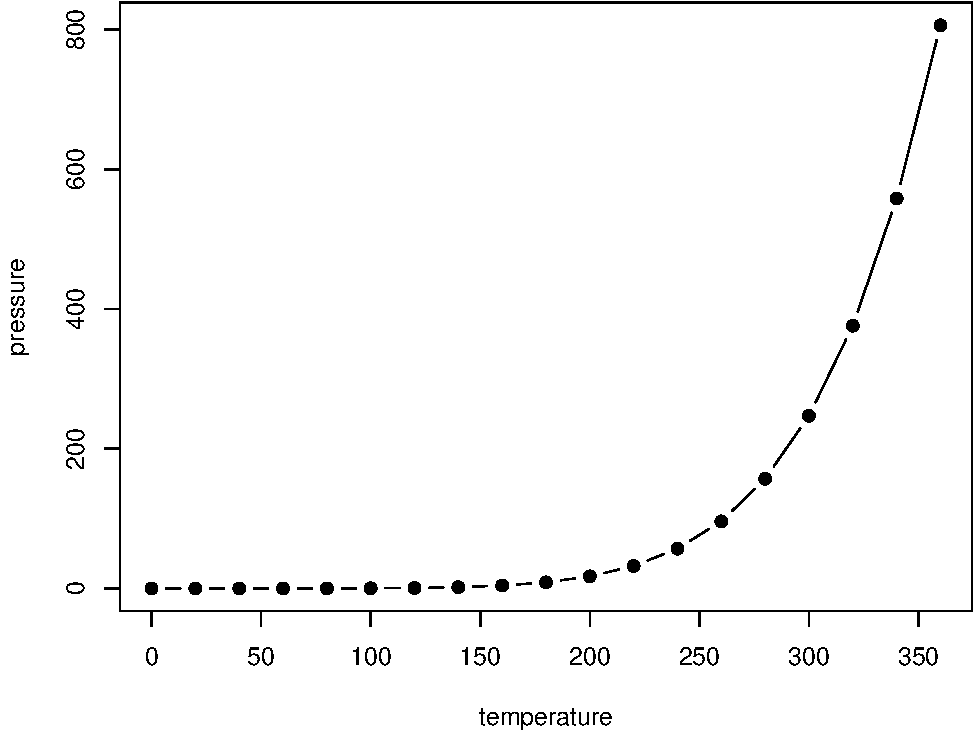
\includegraphics[width=0.8\linewidth]{202401280000-minimal-book-example_files/figure-latex/nice-fig-1} 

}

\caption{Here is a nice figure!}\label{fig:nice-fig}
\end{figure}

Don't miss Table \ref{tab:nice-tab}.

\begin{Shaded}
\begin{Highlighting}[]
\NormalTok{knitr}\SpecialCharTok{::}\FunctionTok{kable}\NormalTok{(}
  \FunctionTok{head}\NormalTok{(pressure, }\DecValTok{10}\NormalTok{), }\AttributeTok{caption =} \StringTok{\textquotesingle{}Here is a nice table!\textquotesingle{}}\NormalTok{,}
  \AttributeTok{booktabs =} \ConstantTok{TRUE}
\NormalTok{)}
\end{Highlighting}
\end{Shaded}

\begin{table}

\caption{\label{tab:nice-tab}Here is a nice table!}
\centering
\begin{tabular}[t]{rr}
\toprule
temperature & pressure\\
\midrule
0 & 0.0002\\
20 & 0.0012\\
40 & 0.0060\\
60 & 0.0300\\
80 & 0.0900\\
\addlinespace
100 & 0.2700\\
120 & 0.7500\\
140 & 1.8500\\
160 & 4.2000\\
180 & 8.8000\\
\bottomrule
\end{tabular}
\end{table}

\section{Parts}\label{parts}

You can add parts to organize one or more book chapters together. Parts can be inserted at the top of an .Rmd file, before the first-level chapter heading in that same file.

Add a numbered part: \texttt{\#\ (PART)\ Act\ one\ \{-\}} (followed by \texttt{\#\ A\ chapter})

Add an unnumbered part: \texttt{\#\ (PART\textbackslash{}*)\ Act\ one\ \{-\}} (followed by \texttt{\#\ A\ chapter})

Add an appendix as a special kind of un-numbered part: \texttt{\#\ (APPENDIX)\ Other\ stuff\ \{-\}} (followed by \texttt{\#\ A\ chapter}). Chapters in an appendix are prepended with letters instead of numbers.

\section{Footnotes and citations}\label{footnotes-and-citations}

\subsection{Footnotes}\label{footnotes}

Footnotes are put inside the square brackets after a caret \texttt{\^{}{[}{]}}. Like this one \footnote{This is a footnote.}.

\subsection{Citations}\label{citations}

Reference items in your bibliography file(s) using \texttt{@key}.

For example, we are using the \textbf{bookdown} package\textsuperscript{\citeproc{ref-R-bookdown}{1}} (check out the last code chunk in index.Rmd to see how this citation key was added) in this sample book, which was built on top of R Markdown and \textbf{knitr}\textsuperscript{\citeproc{ref-xie2015}{2}} (this citation was added manually in an external file book.bib).
Note that the \texttt{.bib} files need to be listed in the index.Rmd with the YAML \texttt{bibliography} key.

The RStudio Visual Markdown Editor can also make it easier to insert citations: \url{https://rstudio.github.io/visual-markdown-editing/\#/citations}

\section{Blocks}\label{blocks}

\subsection{Equations}\label{equations}

Here is an equation.

\begin{equation} 
  f\left(k\right) = \binom{n}{k} p^k\left(1-p\right)^{n-k}
  \label{eq:binom}
\end{equation}

You may refer to using \texttt{\textbackslash{}@ref(eq:binom)}, like see Equation \eqref{eq:binom}.

\subsection{Theorems and proofs}\label{theorems-and-proofs}

Labeled theorems can be referenced in text using \texttt{\textbackslash{}@ref(thm:tri)}, for example, check out this smart theorem \ref{thm:tri}.

\begin{theorem}
\protect\hypertarget{thm:tri}{}\label{thm:tri}For a right triangle, if \(c\) denotes the \emph{length} of the hypotenuse
and \(a\) and \(b\) denote the lengths of the \textbf{other} two sides, we have
\[a^2 + b^2 = c^2\]
\end{theorem}

Read more here \url{https://bookdown.org/yihui/bookdown/markdown-extensions-by-bookdown.html}.

\subsection{Callout blocks}\label{callout-blocks}

The R Markdown Cookbook provides more help on how to use custom blocks to design your own callouts: \url{https://bookdown.org/yihui/rmarkdown-cookbook/custom-blocks.html}

\section{Sharing your book}\label{sharing-your-book}

\subsection{Publishing}\label{publishing}

HTML books can be published online, see: \url{https://bookdown.org/yihui/bookdown/publishing.html}

\subsection{404 pages}\label{pages}

By default, users will be directed to a 404 page if they try to access a webpage that cannot be found. If you'd like to customize your 404 page instead of using the default, you may add either a \texttt{\_404.Rmd} or \texttt{\_404.md} file to your project root and use code and/or Markdown syntax.

\subsection{Metadata for sharing}\label{metadata-for-sharing}

Bookdown HTML books will provide HTML metadata for social sharing on platforms like Twitter, Facebook, and LinkedIn, using information you provide in the \texttt{index.Rmd} YAML. To setup, set the \texttt{url} for your book and the path to your \texttt{cover-image} file. Your book's \texttt{title} and \texttt{description} are also used.

This \texttt{gitbook} uses the same social sharing data across all chapters in your book- all links shared will look the same.

Specify your book's source repository on GitHub using the \texttt{edit} key under the configuration options in the \texttt{\_output.yml} file, which allows users to suggest an edit by linking to a chapter's source file.

Read more about the features of this output format here:

\url{https://pkgs.rstudio.com/bookdown/reference/gitbook.html}

Or use:

\begin{Shaded}
\begin{Highlighting}[]
\NormalTok{?bookdown}\SpecialCharTok{::}\NormalTok{gitbook}
\end{Highlighting}
\end{Shaded}

\chapter{test}\label{test}

\url{https://bookdown.org/yihui/rmarkdown-cookbook/verbatim-code-chunks.html}

\section{RStudio}\label{rstudio}

\subsection{writer options}\label{writer-options}

\url{https://rstudio.github.io/visual-markdown-editing/markdown.html\#writer-options}

\subsubsection{line wrapping}\label{line-wrapping}

\url{https://rstudio.github.io/visual-markdown-editing/markdown.html\#line-wrapping}

\subsubsection{ensuring the same markdown between source / visual mode}\label{ensuring-the-same-markdown-between-source-visual-mode}

\url{https://stackoverflow.com/questions/71775027/rstudio-switch-markdown-editing-mode-between-source-and-visual-changes-special}

\textbf{canonical mode}

\url{https://rstudio.github.io/visual-markdown-editing/markdown.html\#canonical-mode}

\begin{Shaded}
\begin{Highlighting}[]
\PreprocessorTok{{-}{-}{-}}
\FunctionTok{title}\KeywordTok{:}\AttributeTok{ }\StringTok{"My Document"}
\FunctionTok{editor\_options}\KeywordTok{:}
\AttributeTok{  }\FunctionTok{markdown}\KeywordTok{:}
\AttributeTok{    }\FunctionTok{wrap}\KeywordTok{:}\AttributeTok{ }\DecValTok{72}
\AttributeTok{    }\FunctionTok{references}\KeywordTok{:}\AttributeTok{ }
\AttributeTok{      }\FunctionTok{location}\KeywordTok{:}\AttributeTok{ block}
\AttributeTok{    }\FunctionTok{canonical}\KeywordTok{:}\AttributeTok{ }\CharTok{true}
\PreprocessorTok{{-}{-}{-}}
\end{Highlighting}
\end{Shaded}

\subsection{Rtools}\label{rtools}

Rtools43 for Windows
\url{https://cran.r-project.org/bin/windows/Rtools/rtools43/rtools.html}

\subsection{addins}\label{addins}

\url{https://github.com/rstudio/addinexamples}

\begin{verbatim}
if (!requireNamespace("devtools", quietly = TRUE))
  install.packages("devtools")
  
devtools::install_github("rstudio/htmltools")
devtools::install_github("rstudio/shiny")
devtools::install_github("rstudio/miniUI")
\end{verbatim}

\subsection{Git}\label{git}

commit: filename or extension is too long

\url{https://stackoverflow.com/questions/22575662/filename-too-long-in-git-for-windows}

\url{https://stackoverflow.com/questions/55327408/how-to-fix-git-for-windows-error-could-not-lock-config-file-c-file-path-to-g}

\section{RMarkdown}\label{rmarkdown}

\begin{CJK}{UTF8}{bsmi}
R Markdown 指南 https://cosname.github.io/rmarkdown-guide/index.html
\end{CJK}

\url{https://www.rstudio.com/wp-content/uploads/2015/02/rmarkdown-cheatsheet.pdf}

\url{https://slides.yihui.org/2020-taipei-satrday-rmarkdown.html\#1}

\subsection{Pandoc link}\label{pandoc-link}

\url{https://pandoc.org/chunkedhtml-demo/8.16-links-1.html}

\url{https://stackoverflow.com/questions/39281266/use-internal-links-in-rmarkdown-html-output}

\url{https://community.rstudio.com/t/how-to-hyperlink-between-different-rmd-files-in-rmarkdown/62289}

\subsection{URL}\label{url}

\url{https://stackoverflow.com/questions/29787850/how-do-i-add-a-url-to-r-markdown}

\begin{verbatim}
[I'm an inline-style link](https://www.google.com)

[I'm an inline-style link with title](https://www.google.com "Google's Homepage")

[I'm a reference-style link][Arbitrary case-insensitive reference text]

[I'm a relative reference to a repository file](../blob/master/LICENSE)

[You can use numbers for reference-style link definitions][1]

Or leave it empty and use the [link text itself]

Some text to show that the reference links can follow later.

[arbitrary case-insensitive reference text]: https://www.mozilla.org
[1]: http://slashdot.org
[link text itself]: http://www.reddit.com
\end{verbatim}

\subsection{arrow}\label{arrow}

\url{https://reimbar.org/dev/arrows/}

Up arrow: \texttt{\&uarr;}

Down arrow: \texttt{\&darr;}

Left arrow: \texttt{\&larr;}

Right arrow: \texttt{\&rarr;}

Double headed arrow: \texttt{\&harr;}

\subsection{superscript and subscript}\label{superscript-and-subscript}

script\textsuperscript{superscript}\textsubscript{subscript}

\begin{Shaded}
\begin{Highlighting}[]
\NormalTok{script\^{}superscript\^{}}
\end{Highlighting}
\end{Shaded}

script\textsuperscript{superscript}

\begin{Shaded}
\begin{Highlighting}[]
\NormalTok{\textasciitilde{}subscript\textasciitilde{}}
\end{Highlighting}
\end{Shaded}

script\textsubscript{subscript}

\subsubsection{LaTeX}\label{latex}

\url{https://tex.stackexchange.com/questions/580824/subscript-not-distinguished-enough}

\url{https://tex.stackexchange.com/questions/262295/make-subscript-size-smaller-always}

\subsection{equation}\label{equation}

\url{https://stackoverflow.com/questions/26049762/erroneous-nesting-of-equation-structures-in-using-beginalign-in-a-multi-l}

\subsubsection{proof QED}\label{proof-qed}

\url{https://math.meta.stackexchange.com/questions/3582/qed-for-mathjax-here-on-stackexchange}

\texttt{\textbackslash{}tag*\{\$\textbackslash{}Box\$\}}

\[
a^2+b^2=c^2 \tag*{$\Box$}
\]

\texttt{\textbackslash{}tag*\{\$\textbackslash{}blacksquare\$\}}

\[
a^2+b^2=c^2 \tag*{$\blacksquare$}
\]

\subsection{image}\label{image}

\url{https://stackoverflow.com/questions/25166624/insert-picture-table-in-r-markdown}

\subsubsection{DiagrammeR / mermaid flowchart}\label{diagrammer-mermaid-flowchart}

\begin{verbatim}
Error: Functions that produce HTML output found in document targeting latex output.
Please change the output type of this document to HTML.
If your aiming to have some HTML widgets shown in non-HTML format as a screenshot,
please install webshot or webshot2 R package for knitr to do the screenshot.
Alternatively, you can allow HTML output in non-HTML formats
by adding this option to the YAML front-matter of
your rmarkdown file:

  always_allow_html: true

Note however that the HTML output will not be visible in non-HTML formats.
\end{verbatim}

\url{https://bookdown.org/yihui/rmarkdown-cookbook/diagrams.html\#diagrams}

\url{https://stackoverflow.com/questions/40803017/how-to-include-diagrammer-mermaid-flowchart-in-a-rmarkdown-file}

\begin{verbatim}
{r}
library(DiagrammeR)
mermaid("
graph LR
    A-->B
",
width = 100
)
\end{verbatim}

\url{https://github.com/rich-iannone/DiagrammeR/issues/364}

\url{https://stackoverflow.com/questions/55994210/how-to-solve-diagrammer-waste-of-space-issue-in-rmarkdown}

\subsubsection{multiple images / figures in the same line}\label{multiple-images-figures-in-the-same-line}

\url{https://cosname.github.io/rmarkdown-guide/rmarkdown-base.html\#element-figure}

\begin{verbatim}
{r, fig.show = "hold", out.width = "50%"}
plot(cars)
plot(nhtemp)
\end{verbatim}

\begin{Shaded}
\begin{Highlighting}[]
\FunctionTok{plot}\NormalTok{(cars)}
\FunctionTok{plot}\NormalTok{(nhtemp)}
\end{Highlighting}
\end{Shaded}

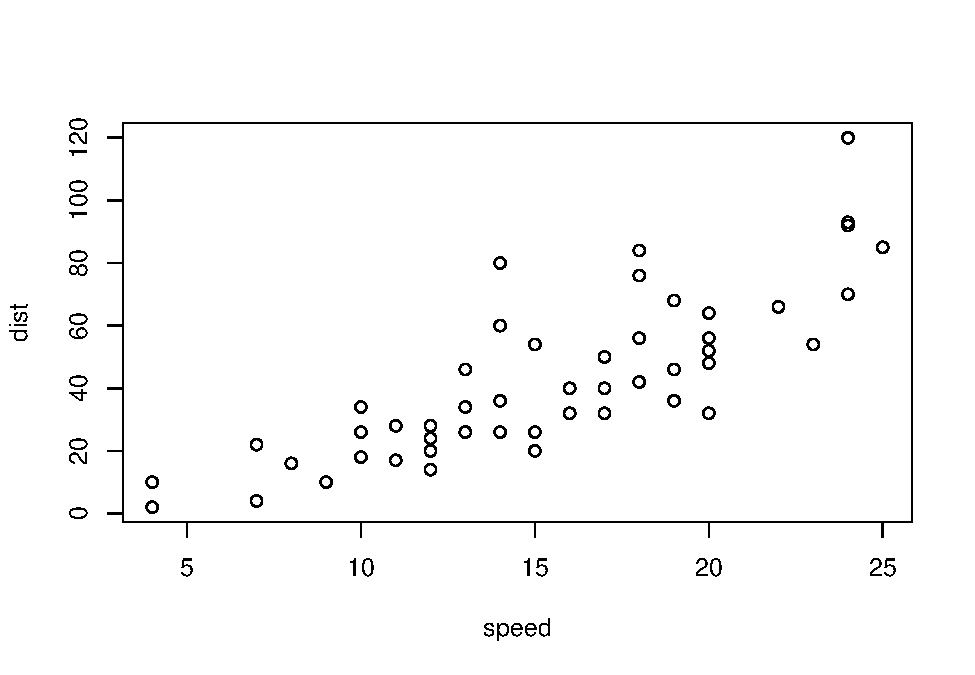
\includegraphics[width=0.5\linewidth]{202401280001-test_files/figure-latex/unnamed-chunk-4-1} 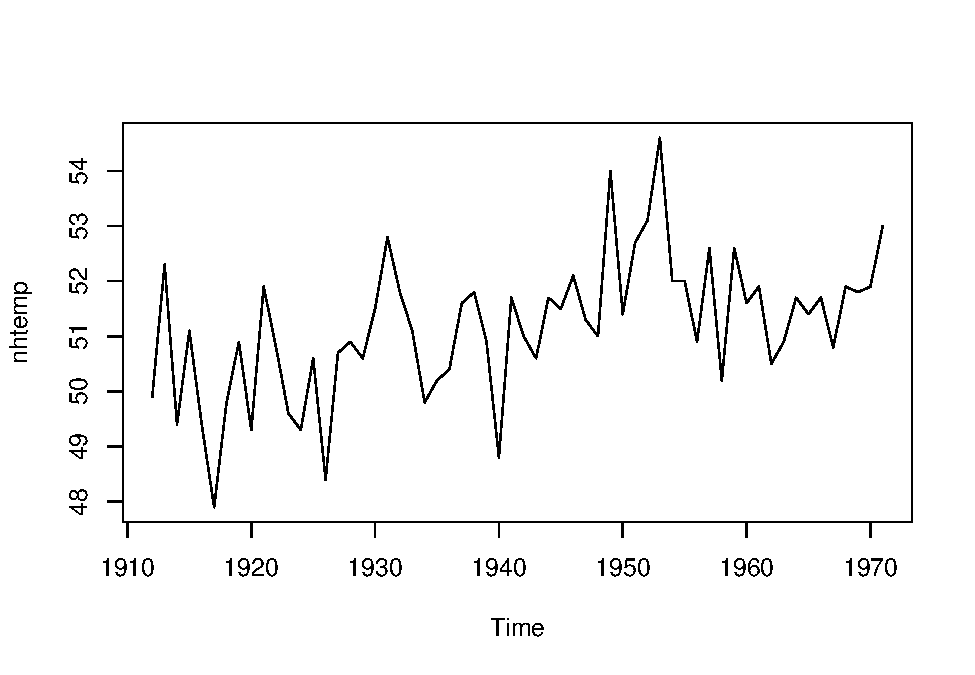
\includegraphics[width=0.5\linewidth]{202401280001-test_files/figure-latex/unnamed-chunk-4-2}

cf.

\begin{verbatim}
{r}
plot(cars)
plot(nhtemp)
\end{verbatim}

\begin{Shaded}
\begin{Highlighting}[]
\FunctionTok{plot}\NormalTok{(cars)}
\end{Highlighting}
\end{Shaded}

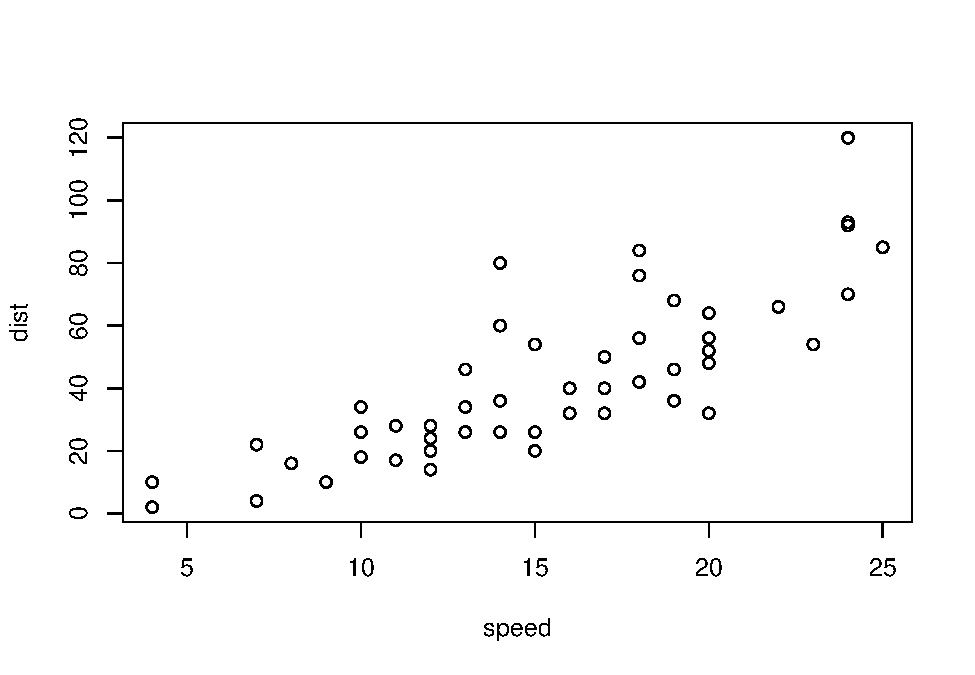
\includegraphics{202401280001-test_files/figure-latex/unnamed-chunk-5-1.pdf}

\begin{Shaded}
\begin{Highlighting}[]
\FunctionTok{plot}\NormalTok{(nhtemp)}
\end{Highlighting}
\end{Shaded}

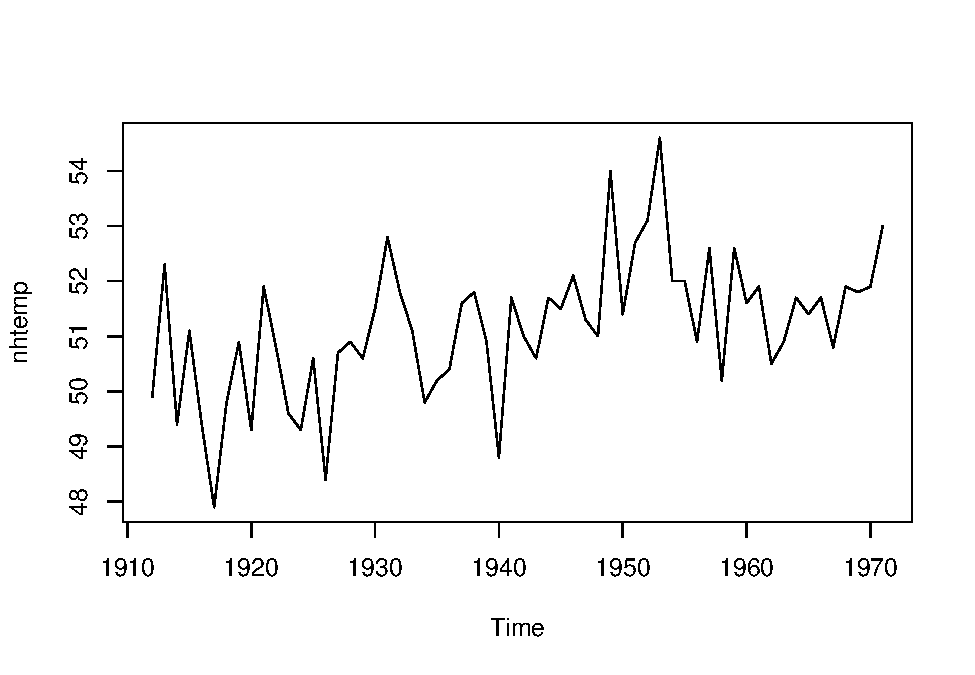
\includegraphics{202401280001-test_files/figure-latex/unnamed-chunk-5-2.pdf}

\subsubsection{figure size}\label{figure-size}

\url{https://sebastiansauer.github.io/figure_sizing_knitr/}

YAML in index.Rmd

\begin{Shaded}
\begin{Highlighting}[]
\PreprocessorTok{{-}{-}{-} }
\FunctionTok{title}\KeywordTok{:}\AttributeTok{ }\StringTok{"My Document"}\AttributeTok{ }
\FunctionTok{output}\KeywordTok{:}\AttributeTok{ html\_document: }
\FunctionTok{fig\_width}\KeywordTok{:}\AttributeTok{ }\DecValTok{6}\AttributeTok{ }
\FunctionTok{fig\_height}\KeywordTok{:}\AttributeTok{ }\DecValTok{4}\AttributeTok{ }
\PreprocessorTok{{-}{-}{-} }
\end{Highlighting}
\end{Shaded}

first R-chunk in your RMD document

\begin{verbatim}
knitr::opts_chunk$set(fig.width=12, fig.height=8) 
\end{verbatim}

width, height and options

\texttt{\textasciigrave{}\textasciigrave{}\textasciigrave{}\{r\ fig.height\ =\ 3,\ fig.width\ =\ 5}

\texttt{plot(pressure)}

\texttt{\textasciigrave{}\textasciigrave{}\textasciigrave{}}

\texttt{\{r\ fig.height\ =\ 3,\ fig.width\ =\ 5}

\begin{Shaded}
\begin{Highlighting}[]
\FunctionTok{plot}\NormalTok{(pressure)}
\end{Highlighting}
\end{Shaded}

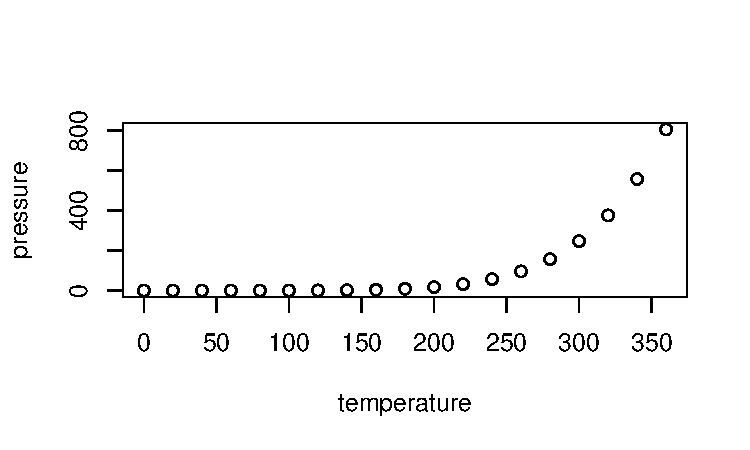
\includegraphics{202401280001-test_files/figure-latex/unnamed-chunk-7-1.pdf}

\texttt{\{r\ fig.height\ =\ 3,\ fig.width\ =\ 3,\ fig.align\ =\ "center"}

\begin{Shaded}
\begin{Highlighting}[]
\FunctionTok{plot}\NormalTok{(pressure)}
\end{Highlighting}
\end{Shaded}

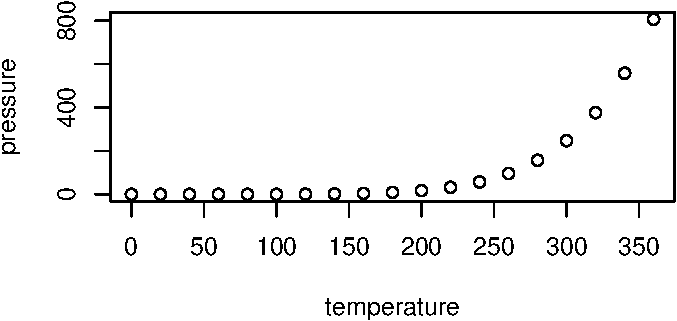
\includegraphics{202401280001-test_files/figure-latex/unnamed-chunk-8-1.pdf}

\texttt{\{r\ fig.width\ =\ 5,\ fig.asp\ =\ .62}

\begin{Shaded}
\begin{Highlighting}[]
\FunctionTok{plot}\NormalTok{(pressure)}
\end{Highlighting}
\end{Shaded}

\begin{center}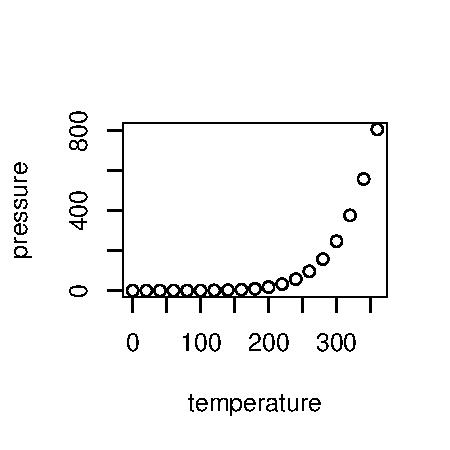
\includegraphics{202401280001-test_files/figure-latex/unnamed-chunk-9-1} \end{center}

\begin{Shaded}
\begin{Highlighting}[]
\DataTypeTok{\textless{}}\KeywordTok{center}\DataTypeTok{\textgreater{}}
\AlertTok{![](https://bookdown.org/yihui/rmarkdown{-}cookbook/images/cover.png)}\NormalTok{\{width=20\%\}}
\DataTypeTok{\textless{}/}\KeywordTok{center}\DataTypeTok{\textgreater{}}
\end{Highlighting}
\end{Shaded}

\paragraph{\texorpdfstring{\texttt{knitr}}{knitr}}\label{knitr}

\url{https://yihui.org/knitr/options/}

\url{https://bookdown.org/yihui/rmarkdown/tufte-figures.html}

\begin{Shaded}
\begin{Highlighting}[]
\FunctionTok{par}\NormalTok{(}\AttributeTok{mar =} \FunctionTok{c}\NormalTok{(}\DecValTok{4}\NormalTok{, }\DecValTok{4}\NormalTok{, .}\DecValTok{1}\NormalTok{, .}\DecValTok{2}\NormalTok{)); }\FunctionTok{plot}\NormalTok{(sunspots)}
\end{Highlighting}
\end{Shaded}

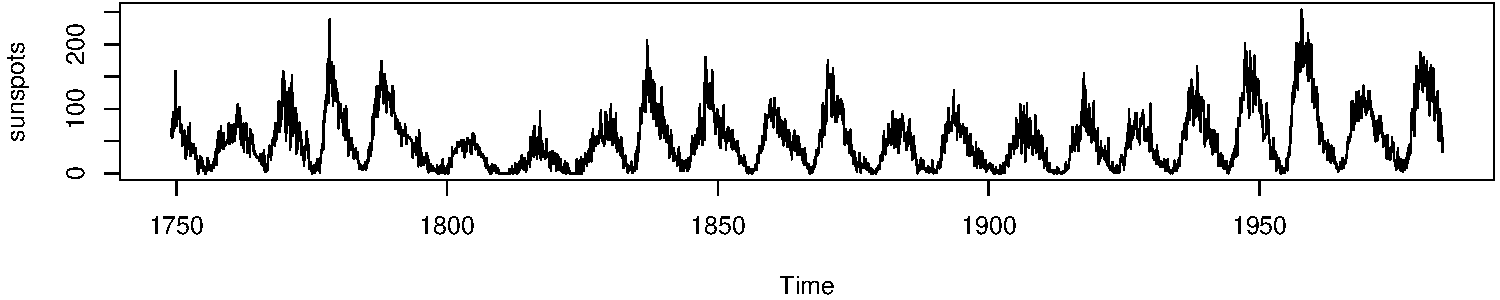
\includegraphics{202401280001-test_files/figure-latex/unnamed-chunk-11-1.pdf}

\begin{Shaded}
\begin{Highlighting}[]
\FunctionTok{plot}\NormalTok{(cars)}
\end{Highlighting}
\end{Shaded}

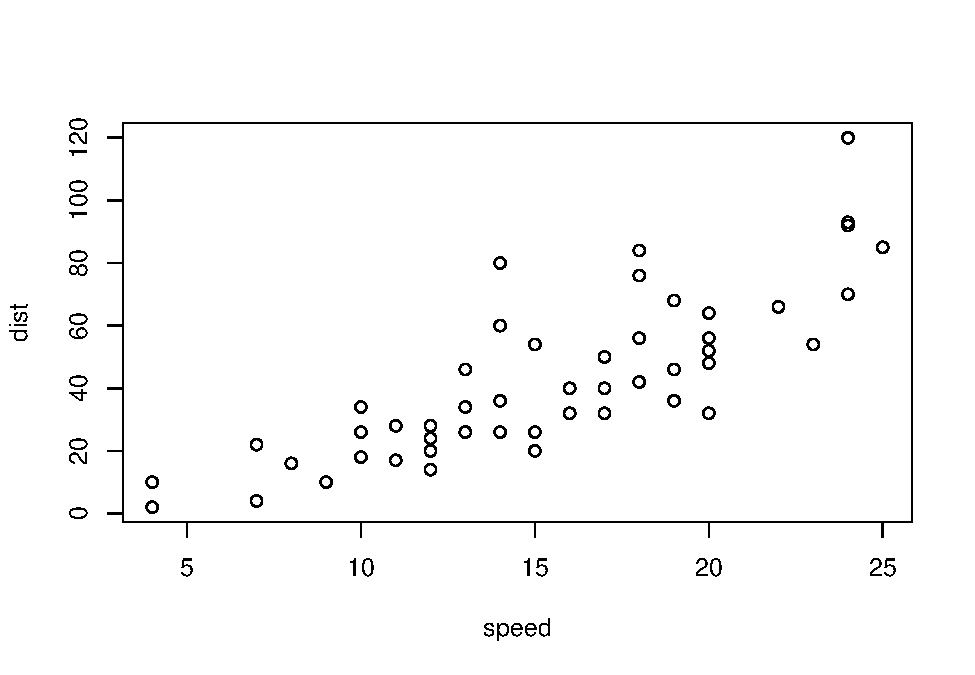
\includegraphics{202401280001-test_files/figure-latex/fig-margin-1.pdf}

\begin{Shaded}
\begin{Highlighting}[]
\NormalTok{We know from \_the first fundamental theorem of calculus\_ that}
\NormalTok{for $x$ in $[a, b]$:}
\NormalTok{$$\textbackslash{}frac\{d\}\{dx\}\textbackslash{}left( \textbackslash{}int\_\{a\}\^{}\{x\} f(u)\textbackslash{},du\textbackslash{}right)=f(x).$$}
\end{Highlighting}
\end{Shaded}

\paragraph{\texorpdfstring{\texttt{out.width} vs.~\texttt{fig.width}}{out.width vs.~fig.width}}\label{out.width-vs.-fig.width}

\url{https://stackoverflow.com/questions/29657777/how-to-make-fig-width-and-out-width-consistent-with-knitr}

when chunk option \texttt{cache=FALSE} is set, then \texttt{out.width} has no effect because no PDF output is created. Hence one has to specify exact measures in inches for \texttt{fig.width} and \texttt{fig.height} for each chunk

\url{https://stackoverflow.com/questions/59567235/a-ggmap-too-small-when-rendered-within-a-rmd-file}

\begin{center}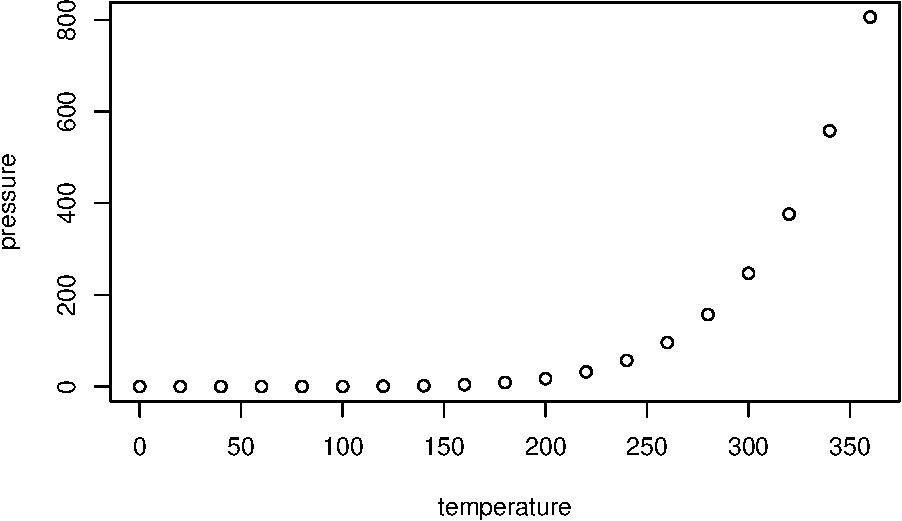
\includegraphics[width=1\linewidth]{202401280001-test_files/figure-latex/unnamed-chunk-13-1} \end{center}

\begin{Shaded}
\begin{Highlighting}[]
\FunctionTok{plot}\NormalTok{(pressure)}
\end{Highlighting}
\end{Shaded}

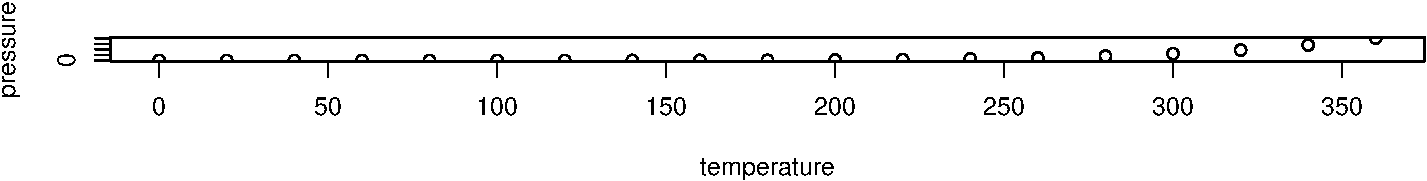
\includegraphics{202401280001-test_files/figure-latex/unnamed-chunk-14-1.pdf}

problem: \texttt{out.width=\textquotesingle{}100\%\textquotesingle{}} causing \texttt{LaTeX\ Error:\ Not\ in\ outer\ par\ mode.}

solution: \texttt{out.width=if\ (knitr:::is\_html\_output())\ \textquotesingle{}100\%\textquotesingle{}}

\begin{cols}

\begin{col}{0.4\textwidth}

\begin{Shaded}
\begin{Highlighting}[]
\KeywordTok{\textbackslash{}begin}\NormalTok{\{}\ExtensionTok{tikzpicture}\NormalTok{\}}
  \FunctionTok{\textbackslash{}draw}\NormalTok{ ({-}1,1){-}{-}(0,0){-}{-}(1,2);}
\KeywordTok{\textbackslash{}end}\NormalTok{\{}\ExtensionTok{tikzpicture}\NormalTok{\}}
\end{Highlighting}
\end{Shaded}

\end{col}

\begin{col}{0.05\textwidth}
~


\end{col}

\begin{col}{0.55\textwidth}
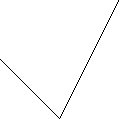
\includegraphics{202401280001-test_files/figure-latex/unnamed-chunk-16-1.pdf}

\end{col}

\end{cols}

\texttt{fig.width=10,\ fig.height=2}

\begin{cols}

\begin{col}{0.4\textwidth}

\begin{Shaded}
\begin{Highlighting}[]
\KeywordTok{\textbackslash{}begin}\NormalTok{\{}\ExtensionTok{tikzpicture}\NormalTok{\}}
  \FunctionTok{\textbackslash{}draw}\NormalTok{ ({-}1,1){-}{-}(0,0){-}{-}(1,2);}
\KeywordTok{\textbackslash{}end}\NormalTok{\{}\ExtensionTok{tikzpicture}\NormalTok{\}}
\end{Highlighting}
\end{Shaded}

\end{col}

\begin{col}{0.05\textwidth}
~


\end{col}

\begin{col}{0.55\textwidth}
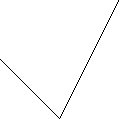
\includegraphics{202401280001-test_files/figure-latex/unnamed-chunk-18-1.pdf}

\end{col}

\end{cols}

\texttt{out.width=if\ (knitr:::is\_html\_output())\ \textquotesingle{}100\%\textquotesingle{}}

\begin{cols}

\begin{col}{0.4\textwidth}

\begin{Shaded}
\begin{Highlighting}[]
\KeywordTok{\textbackslash{}begin}\NormalTok{\{}\ExtensionTok{tikzpicture}\NormalTok{\}}
  \FunctionTok{\textbackslash{}draw}\NormalTok{ ({-}1,1){-}{-}(0,0){-}{-}(1,2);}
\KeywordTok{\textbackslash{}end}\NormalTok{\{}\ExtensionTok{tikzpicture}\NormalTok{\}}
\end{Highlighting}
\end{Shaded}

\end{col}

\begin{col}{0.05\textwidth}
~


\end{col}

\begin{col}{0.55\textwidth}
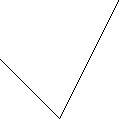
\includegraphics{202401280001-test_files/figure-latex/unnamed-chunk-20-1.pdf}

\end{col}

\end{cols}

\subsubsection{dynamic knitr plot width and height}\label{dynamic-knitr-plot-width-and-height}

\url{https://stackoverflow.com/questions/15365829/dynamic-height-and-width-for-knitr-plots}

\begin{Shaded}
\begin{Highlighting}[]
\FunctionTok{plot}\NormalTok{(pressure)}
\end{Highlighting}
\end{Shaded}

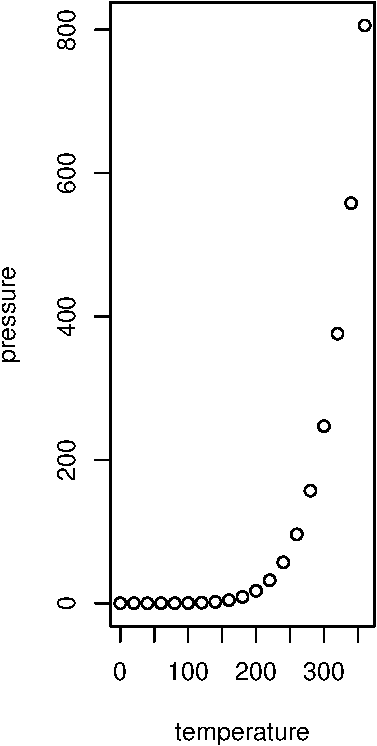
\includegraphics{202401280001-test_files/figure-latex/unnamed-chunk-22-1.pdf}

\subsubsection{web image in PDF}\label{web-image-in-pdf}

\url{https://stackoverflow.com/questions/46331896/how-can-i-insert-an-image-from-internet-to-the-pdf-file-produced-by-r-bookdown-i}

\begin{verbatim}
cover_url = 'https://bookdown.org/yihui/bookdown/images/cover.jpg'
if (!file.exists(cover_file <- xfun::url_filename(cover_url)))
  xfun::download_file(cover_url)
knitr::include_graphics(if (knitr::pandoc_to('html')) cover_url else cover_file)
\end{verbatim}

\begin{figure}
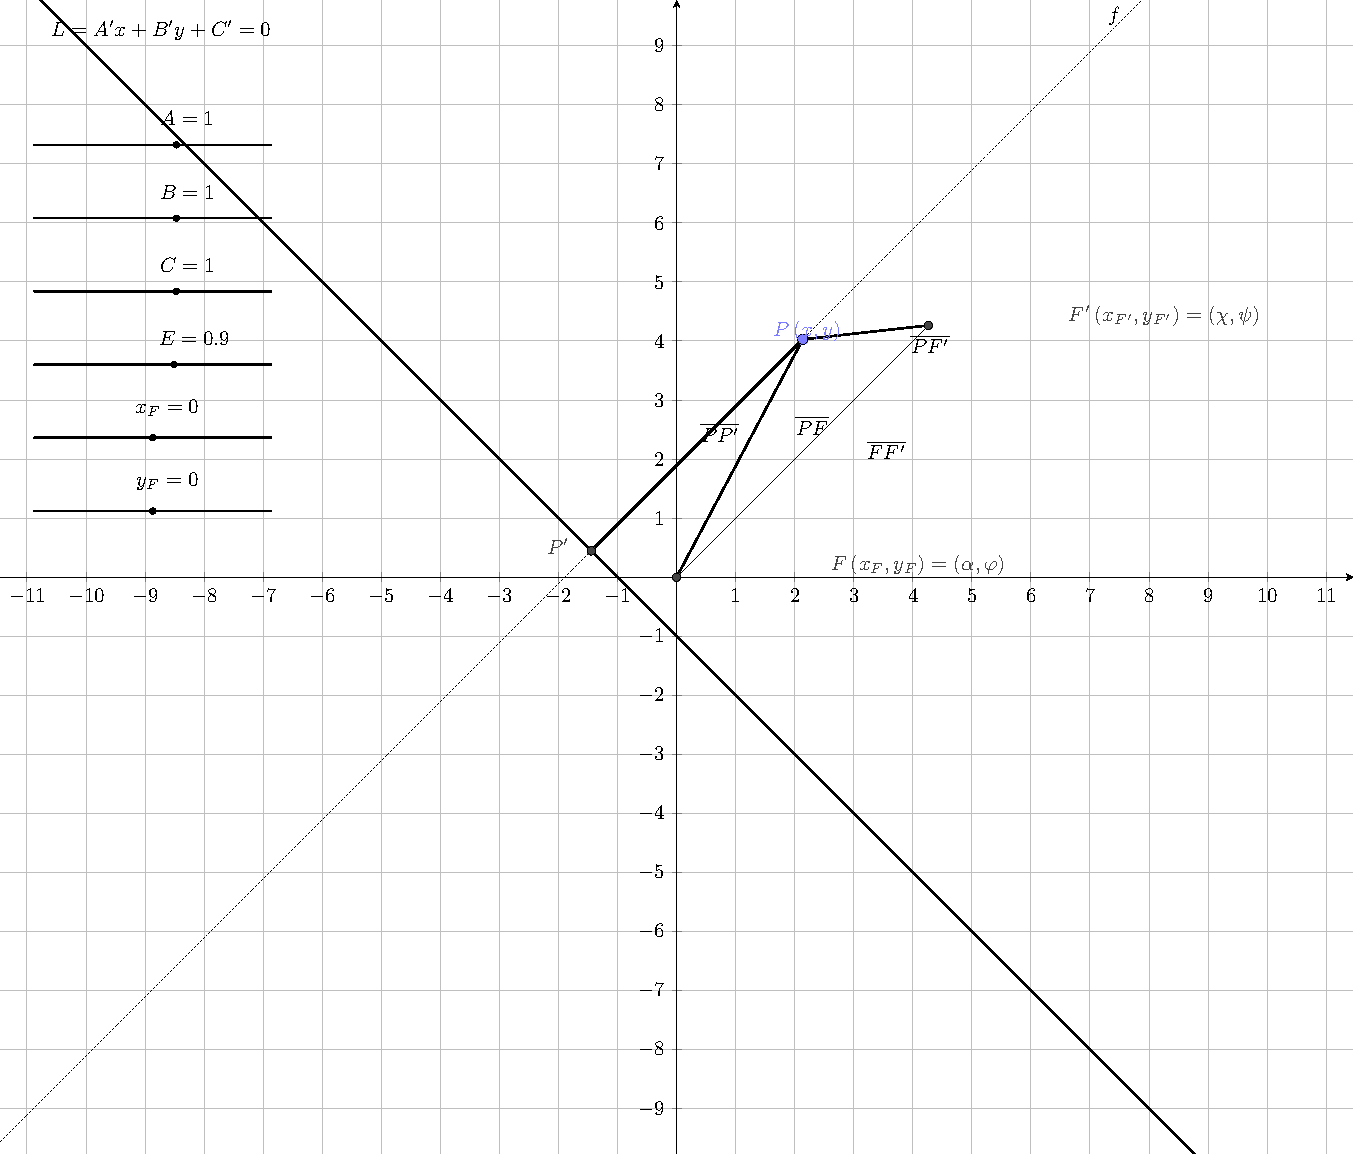
\includegraphics[width=0.75\linewidth]{202401280001-test_files/figure-latex/unnamed-chunk-24-1} \caption{conic sections}\label{fig:unnamed-chunk-24}
\end{figure}

\subsubsection{SVG}\label{svg}

\url{https://stackoverflow.com/questions/50165404/how-to-make-a-pdf-using-bookdown-including-svg-images}

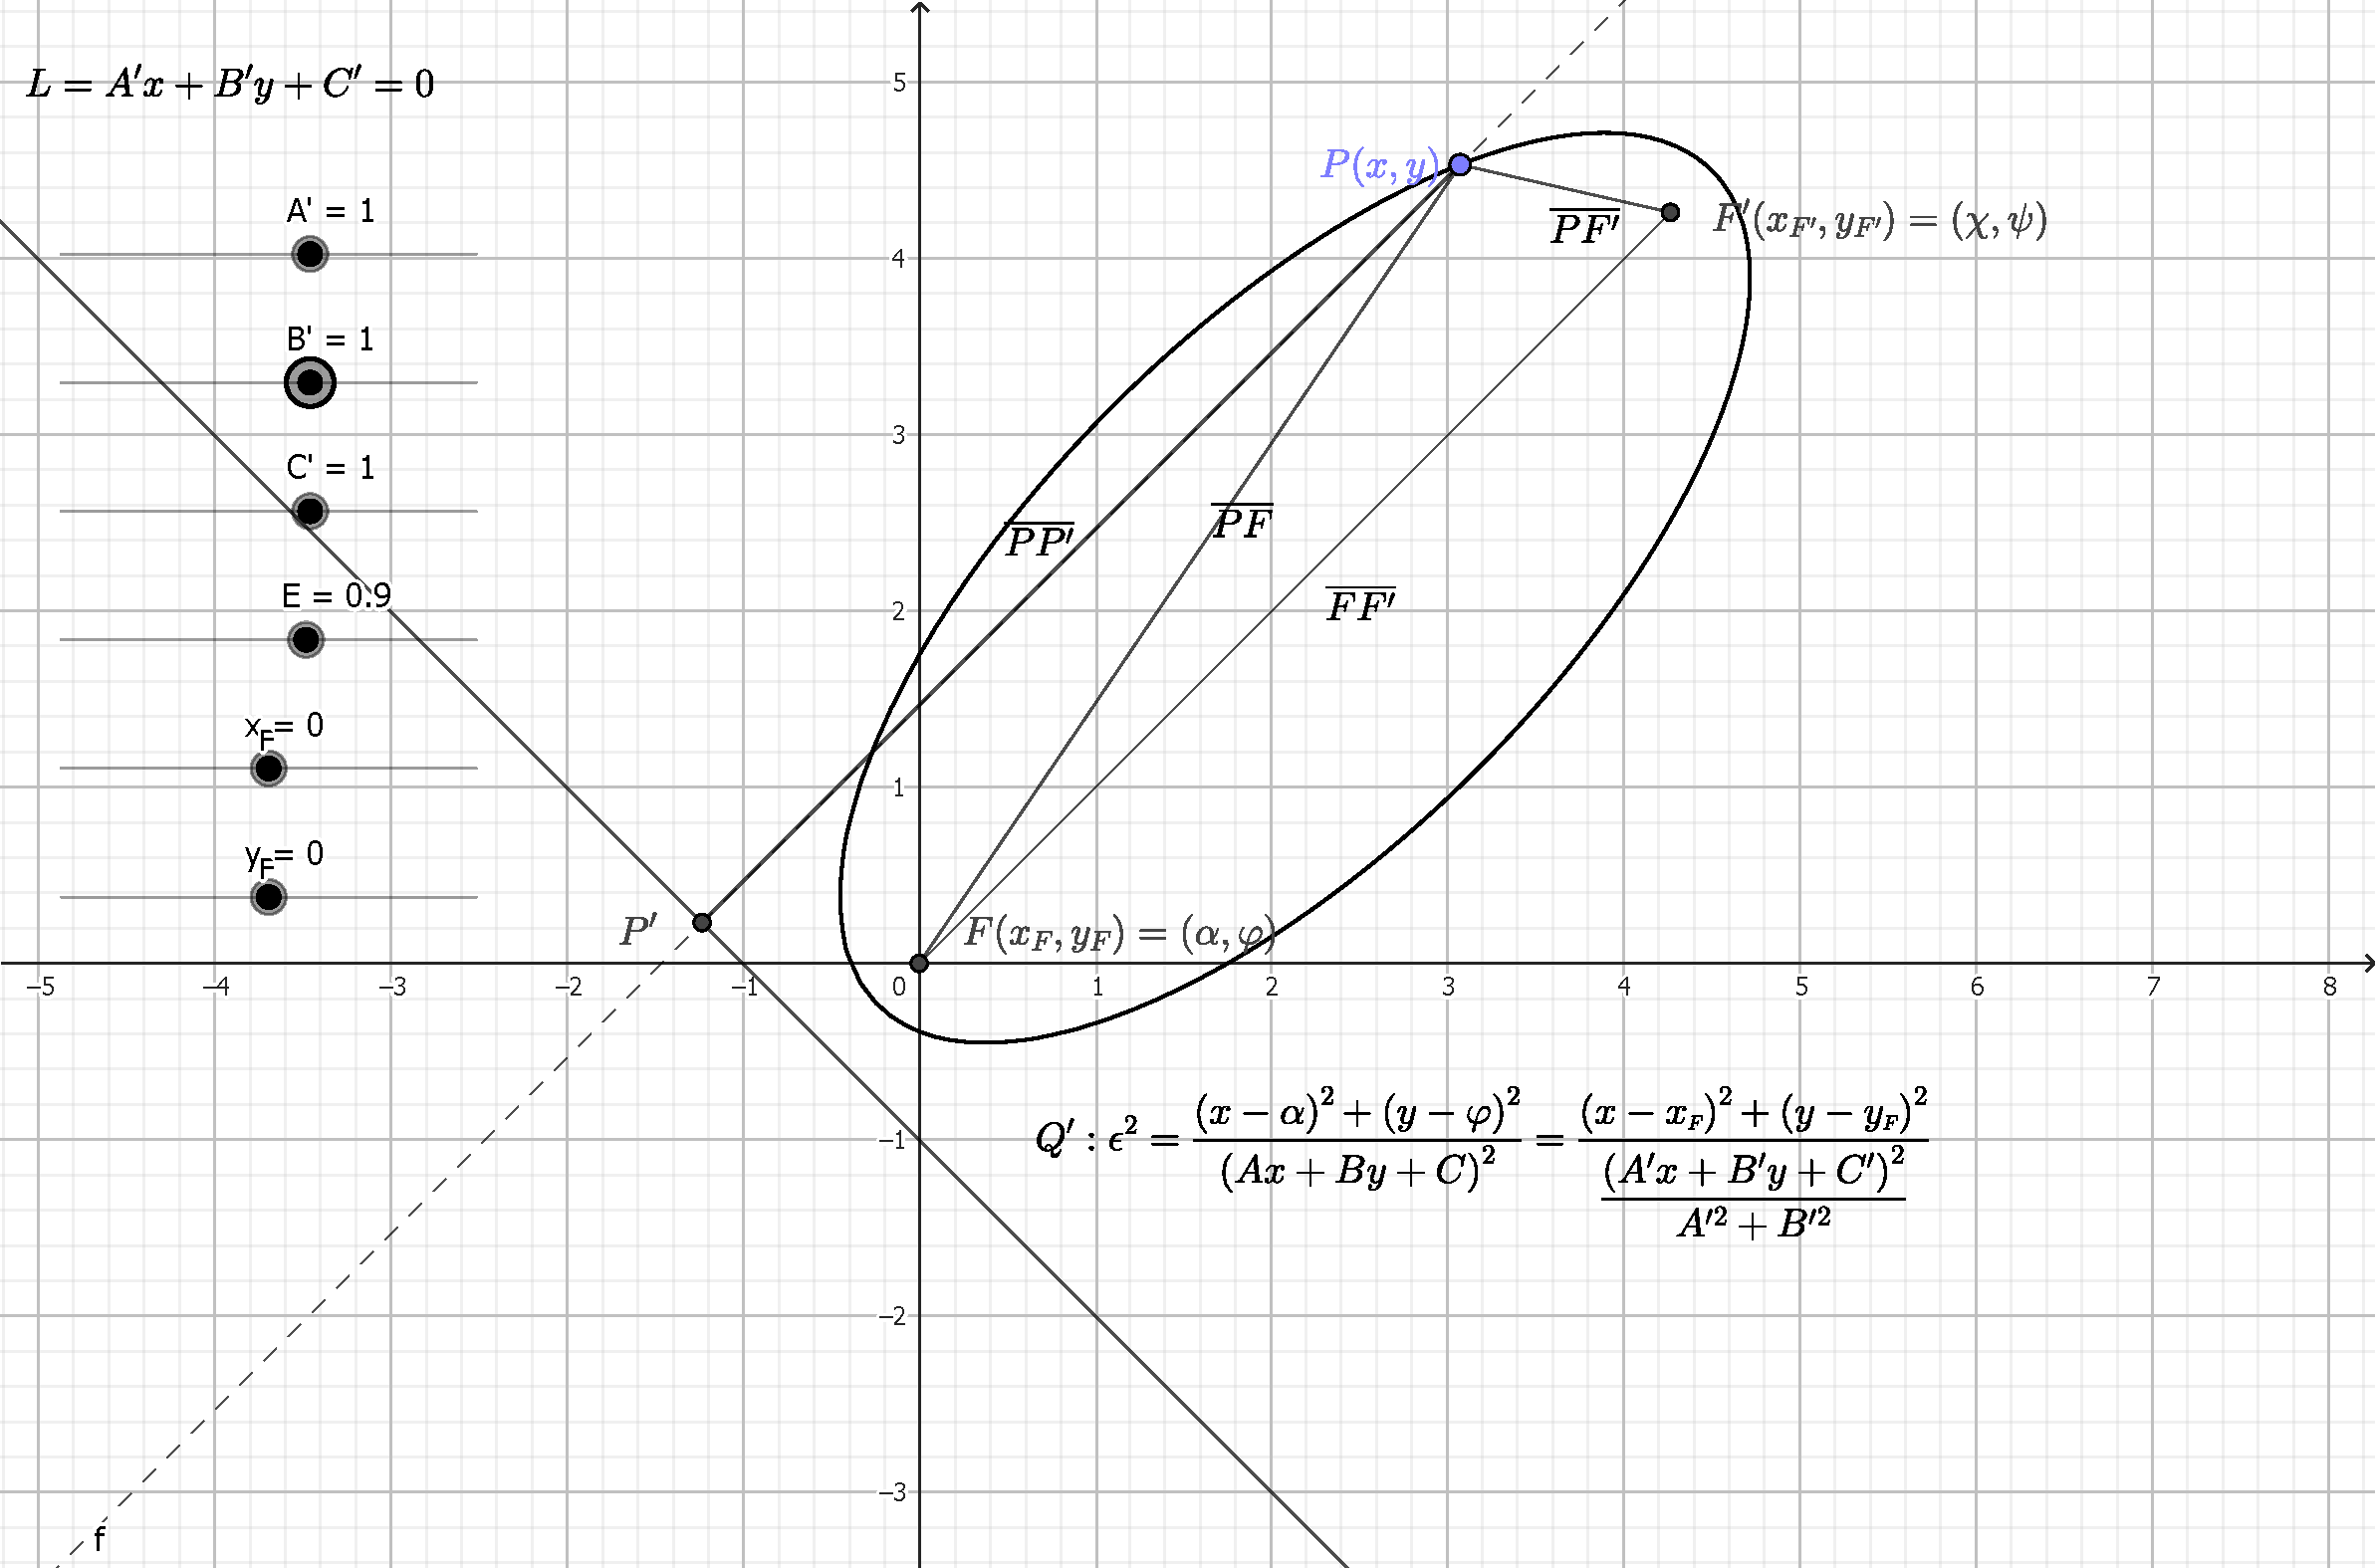
\includegraphics{img/conic-sections.pdf}

\begin{figure}
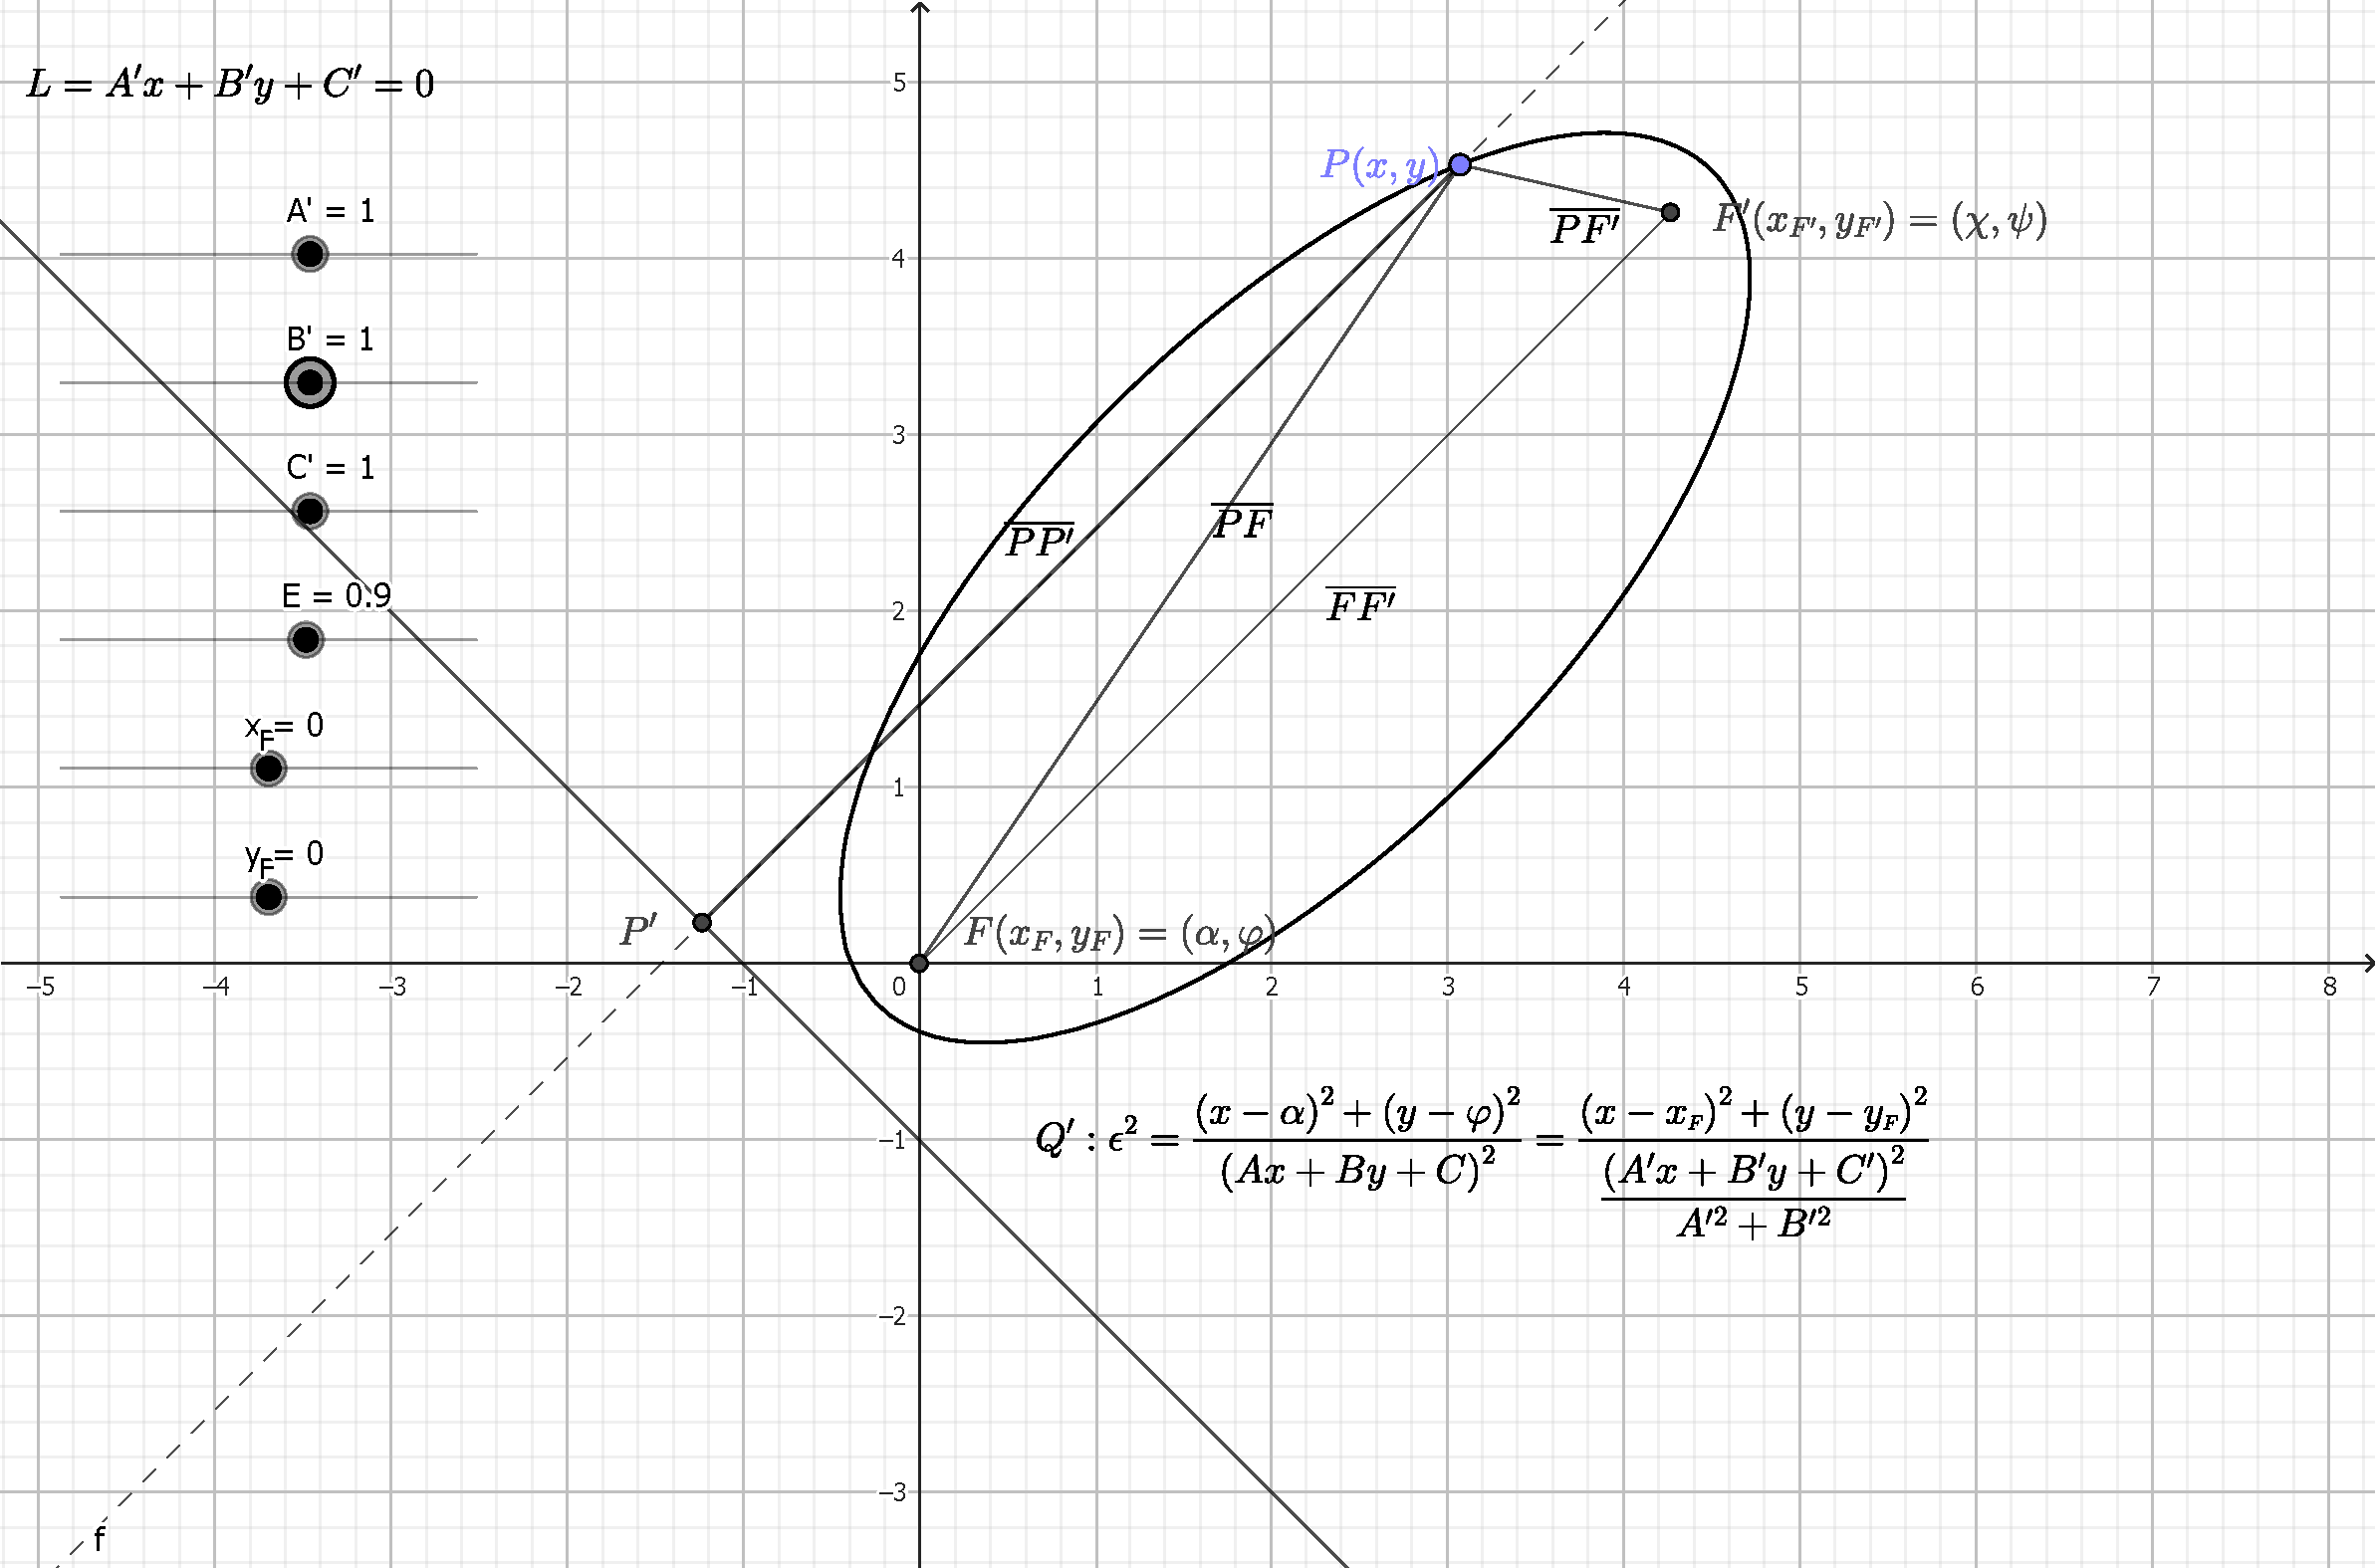
\includegraphics[width=0.75\linewidth]{img/conic-sections} \caption{conic sections}\label{fig:unnamed-chunk-26}
\end{figure}

\url{https://stackoverflow.com/questions/34064292/is-it-possible-to-include-svg-image-in-pdf-document-rendered-by-rmarkdown}

\subsection{horizontal rule}\label{horizontal-rule}

\begin{Shaded}
\begin{Highlighting}[]
\NormalTok{***}
\end{Highlighting}
\end{Shaded}

horizontal rule (or slide break)

\begin{center}\rule{0.5\linewidth}{0.5pt}\end{center}

\begin{Shaded}
\begin{Highlighting}[]
\FunctionTok{dim}\NormalTok{(iris) }
\end{Highlighting}
\end{Shaded}

\begin{verbatim}
## [1] 150   5
\end{verbatim}

\subsection{footnote}\label{footnote}

\subsection{hyperlink}\label{hyperlink}

PDF pandoc internal link will lose focus

\hyperref[equivalence-relation]{equivalence relation} {[}\ref{equivalence-relation}{]} \hyperref[equivalence-relation]{equivalence relation}\footnote{\{\ref{equivalence-relation}\} \hyperref[equivalence-relation]{equivalence relation}} \hyperref[equivalence-relation]{equivalence relation}\textsuperscript{{[}\ref{equivalence-relation}{]}}

\hyperref[equivalence-class]{equivalence class} {[}\ref{equivalence-class}{]} \hyperref[equivalence-class]{equivalence class}\footnote{\{\ref{equivalence-class}\} \hyperref[equivalence-class]{equivalence class}} \hyperref[equivalence-class]{equivalence class}\textsuperscript{{[}\ref{equivalence-class}{]}}

\hyperref[partition]{partition} {[}\ref{partition}{]} \hyperref[partition]{partition}\footnote{\{\ref{partition}\} \hyperref[partition]{partition}} \hyperref[partition]{partition}\textsuperscript{{[}\ref{partition}{]}}

\begin{itemize}
\tightlist
\item
  LaTeX

  \begin{itemize}
  \tightlist
  \item
    \hyperref[tikz]{TikZ}\textsuperscript{{[}\ref{tikz}{]}}

    \begin{itemize}
    \tightlist
    \item
      TikZ-3Dplot
    \item
      PGFplots
    \end{itemize}
  \item
    xypic = \hyperref[xy-pic]{xy-pic}\footnote{\{\ref{xy-pic}\} \hyperref[xy-pic]{xy-pic}}
  \end{itemize}
\item
  OverLeaf
\item
  MathCha
\item
  GeoGebra
\item
  Python

  \begin{itemize}
  \tightlist
  \item
    MatPlotLib
  \item
    Seaborn
  \item
    Plotly
  \end{itemize}
\end{itemize}

\subsection{code chunk}\label{code-chunk}

\subsubsection{code folding}\label{code-folding}

\url{https://cosname.github.io/rmarkdown-guide/rmarkdown-document.html\#html-code-folding}

\subsection{xaringan}\label{xaringan}

slide realtime preview with RStudio addin Infinite Moon Reader in RStudio viewer

\url{https://github.com/yihui/xaringan}

\url{https://www.youtube.com/watch?v=3n9nASHg9gc}

\section{Bookdown}\label{bookdown}

\subsection{system locale}\label{system-locale}

\url{https://bookdown.org/tpemartin/ntpu-programming-for-data-science/appendix-d-.html}

\begin{verbatim}
Sys.getlocale()
\end{verbatim}

Windows

\begin{verbatim}
Sys.setlocale(category = "LC_ALL", locale = "UTF-8")
\end{verbatim}

MacOS

\begin{verbatim}
Sys.setlocale(category = "LC_ALL", locale = "en_US.UTF-8")
\end{verbatim}

\url{https://bookdown.org/yihui/rmarkdown-cookbook/multi-column.html}

\subsection{\texorpdfstring{\texttt{render\_book()}}{render\_book()}}\label{render_book}

\url{https://bookdown.org/yihui/bookdown/build-the-book.html}

\begin{verbatim}
render_book(input = ".", output_format = NULL, ..., clean = TRUE,
  envir = parent.frame(), clean_envir = !interactive(),
  output_dir = NULL, new_session = NA, preview = FALSE,
  config_file = "_bookdown.yml")
\end{verbatim}

\subsection{\texorpdfstring{\texttt{serve\_book()}}{serve\_book()}}\label{serve_book}

\url{https://bookdown.org/yihui/bookdown/serve-the-book.html}

\begin{verbatim}
serve_book(dir = ".", output_dir = "_book", preview = TRUE,
  in_session = TRUE, quiet = FALSE, ...)
\end{verbatim}

\subsection{LaTeX}\label{latex-1}

\subsubsection{hyperlink, URL, href}\label{hyperlink-url-href}

\url{https://www.baeldung.com/cs/latex-hyperref-url-hyperlinks}

\begin{CJK}{UTF8}{bsmi}
https://www.omdte.com/小技巧讓-facebook和-line顯示中文網址,網址不再變亂碼/
\end{CJK}

\subsubsection{\texorpdfstring{ugly mathptmx \(\sum\)}{ugly mathptmx \textbackslash sum}}\label{ugly-mathptmx-sum}

PDF LaTeX \texttt{\textbackslash{}usepackage\{fdsymbol\}} to have \texttt{\textbackslash{}overrightharpoon} vector; however, there are too many side effects, including ugly mathptmx \(\sum\), \ldots{}

\begin{verbatim}

\usepackage{fdsymbol} % vector over accent, but will use mathptmx
% replace the rather ugly mathptmx \sum operator with the equivalent Computer Modern one
\let\sum\relax
\DeclareSymbolFont{CMlargesymbols}{OMX}{cmex}{m}{n}
\DeclareMathSymbol{\sum}{\mathop}{CMlargesymbols}{"50}
\end{verbatim}

\url{https://tex.stackexchange.com/questions/315102/different-sum-signs}

\url{https://tex.stackexchange.com/questions/275038/how-to-replace-mathptmx-sum-with-cm-sum}

\url{https://tex.stackexchange.com/questions/391410/calligraphic-symbols-are-too-fancy-with-mathptmx-package}

\url{https://blog.csdn.net/kongtaoxing/article/details/131005044}

In \texttt{preamble.tex}, add

\begin{verbatim}

% replace the rather ugly mathptmx \sum operator with the equivalent Computer Modern one
\let\sum\relax
\DeclareSymbolFont{CMlargesymbols}{OMX}{cmex}{m}{n}
\DeclareMathSymbol{\sum}{\mathop}{CMlargesymbols}{"50}

\DeclareMathAlphabet{\mathcal}{OMS}{cmsy}{m}{n}
\DeclareSymbolFont{largesymbols}{OMX}{cmex}{m}{n}
\end{verbatim}

\subsubsection{LaTeX package in HTML document}\label{latex-package-in-html-document}

\url{https://github.com/rstudio/rmarkdown/issues/1829}

\begin{verbatim}
---
title: "assignment"
author: "author"
output: html_document
---

$$
  \require{cancel}
  \cancel{x}
$$
\end{verbatim}

\[
  \cancel{x}
\]

\url{https://stackoverflow.com/questions/18189175/how-to-use-textup-with-mathjax}

\begin{quote}
\texttt{\textbackslash{}textup} is not available in MathJax. You can replace it with \texttt{\textbackslash{}mathrm}, \textbf{but \texttt{\textbackslash{}mathrm} does not interpret spaces}.
\end{quote}

\subsection{\texorpdfstring{depth of table of contents \texttt{toc\_depth}}{depth of table of contents toc\_depth}}\label{depth-of-table-of-contents-toc_depth}

\url{https://stackoverflow.com/questions/49009212/how-to-change-toc-depth-in-r-bookdown-gitbook}

\begin{Shaded}
\begin{Highlighting}[]
\AttributeTok{bookdown:}\FunctionTok{:gitbook}\KeywordTok{:}
\AttributeTok{    }\FunctionTok{toc\_depth}\KeywordTok{:}\AttributeTok{ }\DecValTok{2}
\end{Highlighting}
\end{Shaded}

\url{https://stackoverflow.com/questions/68537309/how-can-i-specific-the-initial-level-to-have-my-table-of-contents-be-expanded-to}

\begin{Shaded}
\begin{Highlighting}[]
\FunctionTok{toc}\KeywordTok{:}
\AttributeTok{  }\FunctionTok{collapse}\KeywordTok{:}\AttributeTok{ section}
\end{Highlighting}
\end{Shaded}

\subsection{multi-column layout / two columns}\label{multi-column}

\url{https://bookdown.org/yihui/rmarkdown-cookbook/multi-column.html}

\subsubsection{for both HTML and PDF}\label{for-both-html-and-pdf}

\hyperref[figure-size]{figure size}\textsuperscript{{[}\ref{figure-size}{]}}

\begin{quote}
Below is a Div containing three child Divs side by side. The Div in the middle is empty, just to add more space between the left and right Divs.
\end{quote}

\begin{verbatim}
:::::: {.cols data-latex=""}

::: {.col data-latex="{0.55\textwidth}"}
![](202401280001-test_files/figure-latex/unnamed-chunk-32-1.pdf)<!-- --> 
:::

::: {.col data-latex="{0.05\textwidth}"}
\ 
<!-- an empty Div (with a white space), serving as
a column separator -->
:::

::: {.col data-latex="{0.4\textwidth}"}
The figure on the left-hand side shows the `cars` data.

Lorem ipsum dolor sit amet, consectetur adipiscing elit, sed do
eiusmod tempor incididunt ut labore et dolore magna aliqua. Ut
enim ad minim veniam, quis nostrud exercitation ullamco laboris
nisi ut aliquip ex ea commodo consequat. Duis aute irure dolor
in reprehenderit in voluptate velit esse cillum dolore eu fugiat
nulla pariatur.
:::
::::::
\end{verbatim}

\texttt{\{r,\ echo=FALSE,\ fig.width=5,\ fig.height=4\}}

\begin{cols}

\begin{col}{0.55\textwidth}
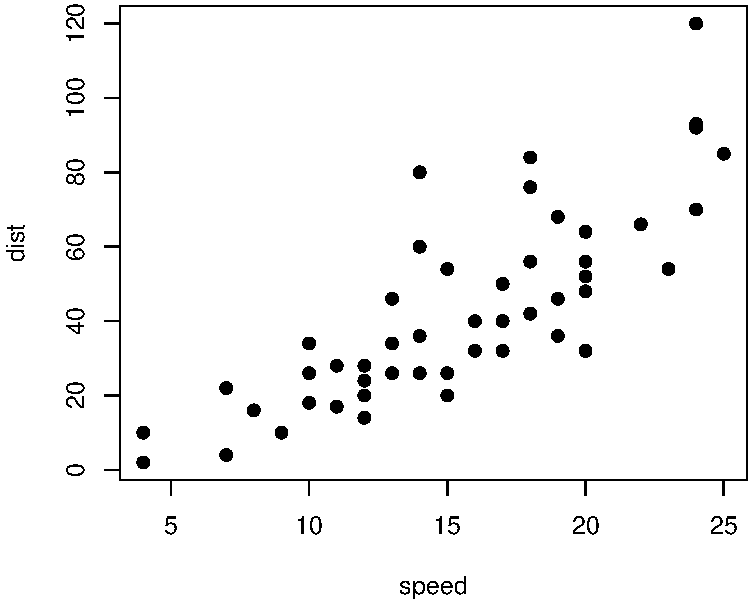
\includegraphics{202401280001-test_files/figure-latex/unnamed-chunk-33-1.pdf}

\end{col}

\begin{col}{0.05\textwidth}
~


\end{col}

\begin{col}{0.4\textwidth}
The figure on the left-hand side shows the \texttt{cars} data.

Lorem ipsum dolor sit amet, consectetur adipiscing elit, sed do
eiusmod tempor incididunt ut labore et dolore magna aliqua. Ut
enim ad minim veniam, quis nostrud exercitation ullamco laboris
nisi ut aliquip ex ea commodo consequat. Duis aute irure dolor
in reprehenderit in voluptate velit esse cillum dolore eu fugiat
nulla pariatur.

\end{col}

\end{cols}

\texttt{\{r,\ echo=FALSE,\ fig.width=10,\ fig.height=8,\ out.width\ =\ "100\%"\}}

\begin{cols}

\begin{col}{0.55\textwidth}
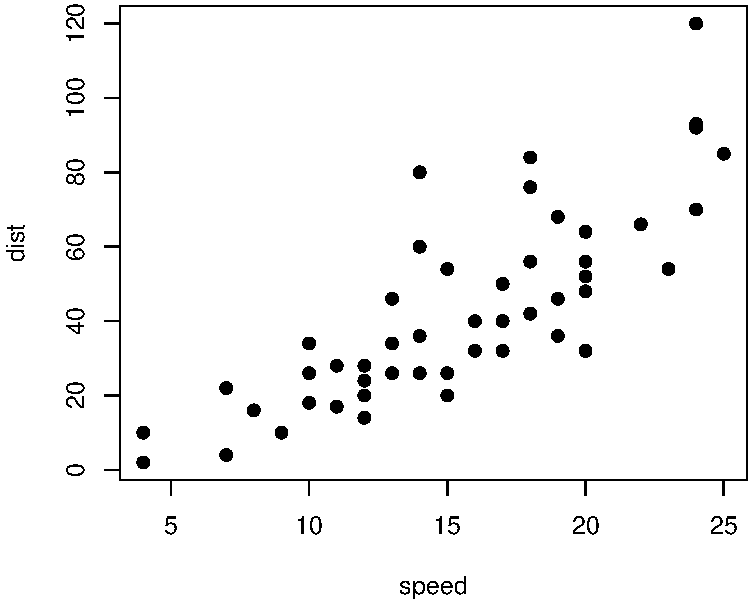
\includegraphics[width=1\linewidth]{202401280001-test_files/figure-latex/unnamed-chunk-34-1}

\end{col}

\begin{col}{0.05\textwidth}
~


\end{col}

\begin{col}{0.4\textwidth}
The figure on the left-hand side shows the \texttt{cars} data.

Lorem ipsum dolor sit amet, consectetur adipiscing elit, sed do
eiusmod tempor incididunt ut labore et dolore magna aliqua. Ut
enim ad minim veniam, quis nostrud exercitation ullamco laboris
nisi ut aliquip ex ea commodo consequat. Duis aute irure dolor
in reprehenderit in voluptate velit esse cillum dolore eu fugiat
nulla pariatur.

\end{col}

\end{cols}

\texttt{\{r,\ echo=FALSE,\ fig.width=10,\ fig.height=8\}}

\begin{cols}

\begin{col}{0.55\textwidth}
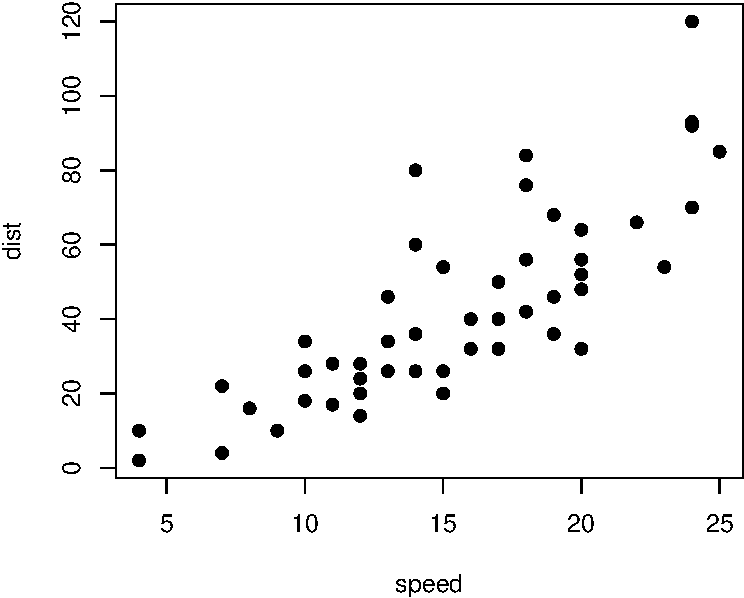
\includegraphics{202401280001-test_files/figure-latex/unnamed-chunk-35-1.pdf}

\end{col}

\begin{col}{0.05\textwidth}
~


\end{col}

\begin{col}{0.4\textwidth}
The figure on the left-hand side shows the \texttt{cars} data.

Lorem ipsum dolor sit amet, consectetur adipiscing elit, sed do
eiusmod tempor incididunt ut labore et dolore magna aliqua. Ut
enim ad minim veniam, quis nostrud exercitation ullamco laboris
nisi ut aliquip ex ea commodo consequat. Duis aute irure dolor
in reprehenderit in voluptate velit esse cillum dolore eu fugiat
nulla pariatur.

\end{col}

\end{cols}

\subsubsection{\texorpdfstring{multi-column \texttt{fig.cap} must use \texttt{fig.pos="H"}}{multi-column fig.cap must use fig.pos="H"}}\label{multi-column-fig.cap-must-use-fig.posh}

\url{https://community.rstudio.com/t/adding-fig-cap-caption-text-to-code-chunk-causes-figure-to-print-at-top-of-page-instead-of-where-it-should-be/30297}

\url{https://bookdown.org/yihui/rmarkdown-cookbook/figure-placement.html}

to avoid \texttt{LaTeX\ Error:\ Not\ in\ outer\ par\ mode} for caption in multi-column LaTeX PDF

in \texttt{output.yml} add \texttt{extra\_dependencies:\ {[}"float"{]}} under \texttt{bookdown::pdf\_book:}

include first chunk \texttt{knitr::opts\_chunk\$set(fig.pos\ =\ "H",\ out.extra\ =\ "")} in .Rmd

add \texttt{out.width=if\ (knitr:::is\_html\_output())\ \textquotesingle{}50\%\textquotesingle{}} for TikZ chunk

thus complete chunk beginning with \texttt{\{r,\ echo=FALSE,\ cache=TRUE,\ engine=\textquotesingle{}tikz\textquotesingle{},\ fig.ext=if\ (knitr:::is\_latex\_output())\ \textquotesingle{}pdf\textquotesingle{}\ else\ \textquotesingle{}png\textquotesingle{},\ fig.width=10,\ fig.height=2,\ out.width=if\ (knitr:::is\_html\_output())\ \textquotesingle{}100\%\textquotesingle{},\ fig.cap=\textquotesingle{}\textquotesingle{}\}}

\begin{cols}

\begin{col}{0.45\textwidth}

\begin{Shaded}
\begin{Highlighting}[]
\KeywordTok{\textbackslash{}begin}\NormalTok{\{}\ExtensionTok{tikzpicture}\NormalTok{\}}
  \FunctionTok{\textbackslash{}draw}\NormalTok{ ({-}1,1){-}{-}(0,0){-}{-}(1,2);}
\KeywordTok{\textbackslash{}end}\NormalTok{\{}\ExtensionTok{tikzpicture}\NormalTok{\}}
\end{Highlighting}
\end{Shaded}

\end{col}

\begin{col}{0.10\textwidth}
~

\end{col}

\begin{col}{0.45\textwidth}
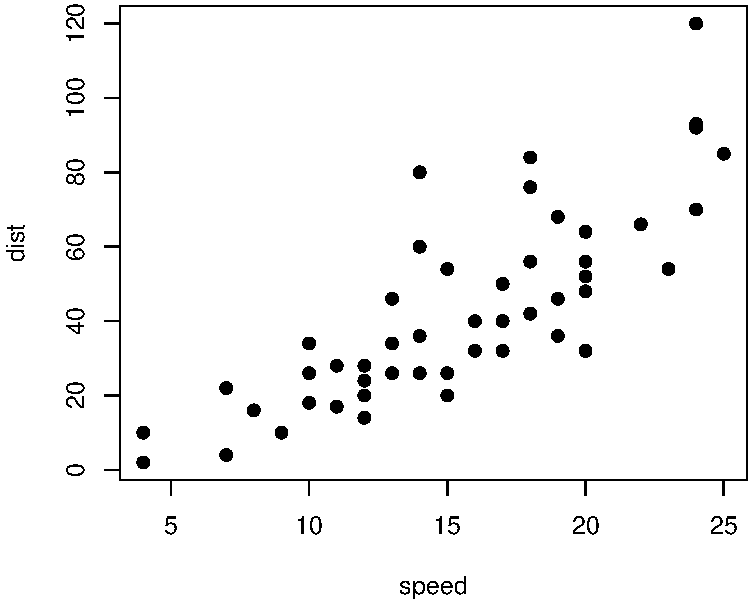
\includegraphics{202401280001-test_files/figure-latex/unnamed-chunk-37-1.pdf}

\end{col}

\end{cols}

LaTeX package \texttt{caption}

\url{https://tex.stackexchange.com/questions/128485/how-to-make-a-caption-via-captionof-and-extra-margins-adhere-to-minipage-marg}

What is the different between using \texttt{\textbackslash{}captionof\{table\}\{ABC\}} and \texttt{\textbackslash{}caption\{ABC\}}?

\url{https://tex.stackexchange.com/questions/514286/what-is-the-different-between-using-captionoftableabc-and-captionabc}

side-by-side table

\url{https://stackoverflow.com/questions/73745714/how-to-print-gt-tbl-tables-side-by-side-with-knitr-kable}

R ternary operator

\url{https://stackoverflow.com/questions/8790143/does-the-ternary-operator-exist-in-r}

\subsubsection{caption above figure}\label{caption-above-figure}

\url{https://stackoverflow.com/questions/56979022/caption-above-figure-in-html-rmarkdown}

\texttt{fig.topcaption=TRUE}

\subsubsection{for only HTML}\label{for-only-html}

\paragraph{CSS flex}\label{css-flex}

Here is the \textbf{first} Div.

\begin{Shaded}
\begin{Highlighting}[]
\FunctionTok{str}\NormalTok{(iris)}
\end{Highlighting}
\end{Shaded}

\begin{verbatim}
## 'data.frame':    150 obs. of  5 variables:
##  $ Sepal.Length: num  5.1 4.9 4.7 4.6 5 5.4 4.6 5 4.4 4.9 ...
##  $ Sepal.Width : num  3.5 3 3.2 3.1 3.6 3.9 3.4 3.4 2.9 3.1 ...
##  $ Petal.Length: num  1.4 1.4 1.3 1.5 1.4 1.7 1.4 1.5 1.4 1.5 ...
##  $ Petal.Width : num  0.2 0.2 0.2 0.2 0.2 0.4 0.3 0.2 0.2 0.1 ...
##  $ Species     : Factor w/ 3 levels "setosa","versicolor",..: 1 1 1 1 1 1 1 1 1 1 ...
\end{verbatim}

And this block will be put on the right:

\begin{Shaded}
\begin{Highlighting}[]
\FunctionTok{plot}\NormalTok{(iris[, }\SpecialCharTok{{-}}\DecValTok{5}\NormalTok{])}
\end{Highlighting}
\end{Shaded}

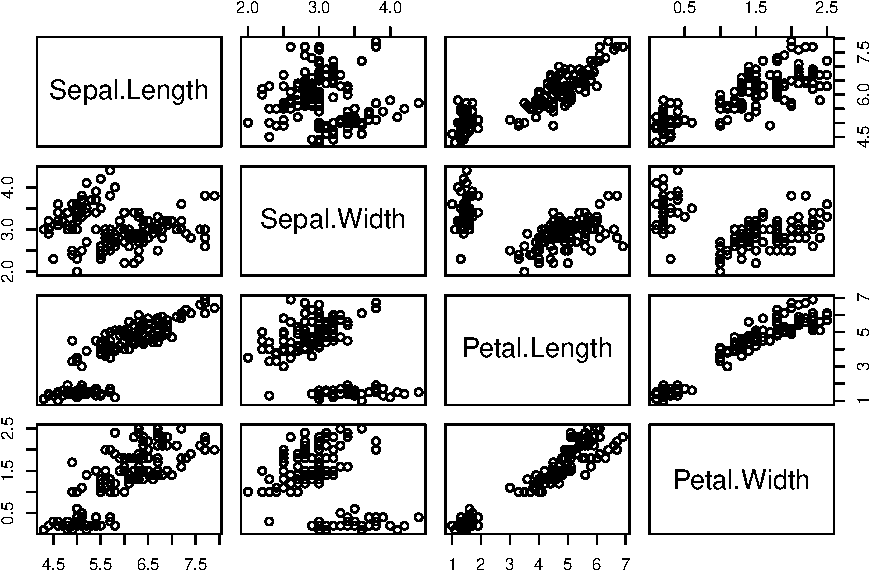
\includegraphics{202401280001-test_files/figure-latex/unnamed-chunk-39-1.pdf}

\paragraph{CSS grid}\label{css-grid}

\url{https://github.com/yihui/knitr/issues/1743}

\begin{CJK}{UTF8}{bsmi}
https://medium.com/enjoy-life-enjoy-coding/css-所以我說那個版能不能好切一點-grid-基本用法-cd763091cf70
\end{CJK}

\begin{Shaded}
\begin{Highlighting}[]
\FunctionTok{head}\NormalTok{(iris)}
\end{Highlighting}
\end{Shaded}

\begin{verbatim}
##   Sepal.Length Sepal.Width Petal.Length Petal.Width Species
## 1          5.1         3.5          1.4         0.2  setosa
## 2          4.9         3.0          1.4         0.2  setosa
## 3          4.7         3.2          1.3         0.2  setosa
## 4          4.6         3.1          1.5         0.2  setosa
## 5          5.0         3.6          1.4         0.2  setosa
## 6          5.4         3.9          1.7         0.4  setosa
\end{verbatim}

\begin{Shaded}
\begin{Highlighting}[]
\FunctionTok{plot}\NormalTok{(iris)}
\end{Highlighting}
\end{Shaded}

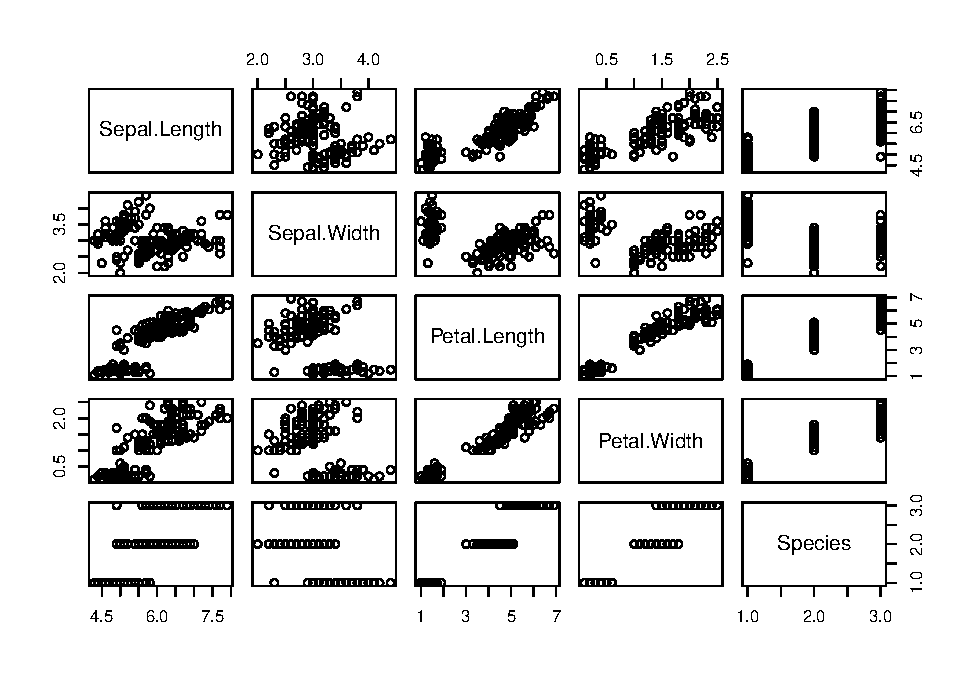
\includegraphics{202401280001-test_files/figure-latex/unnamed-chunk-41-1.pdf}

\section{conditional block/chunk for either HTML or PDF, and Chinese issue}\label{conditional-blockchunk-for-either-html-or-pdf-and-chinese-issue}

\url{https://stackoverflow.com/questions/76240244/bookdown-conditional-display-of-text-and-code-blocks-latex-pdf-vs-html}

\begin{CJK}{UTF8}{bsmi}等價關係 equivalence relation \label{def:equivalence-relation}
\end{CJK}
\begin{CJK}{UTF8}{bsmi}
\begin{align*}
 & R\text{ is an equivalence relation over }A\times B\\
\Leftrightarrow & \begin{cases}
R=\sim=\left\{ \left\langle x,y\right\rangle \middle|x\sim y\right\} \subseteq A\times B & \left(\text{e}\right)\text{equivalence 等價}\\
\vdots & \vdots
\end{cases}\\
\Leftrightarrow & \begin{cases}
R=\left\{ \left\langle x,y\right\rangle \middle|xRy\right\} \subseteq A\times B & \left(R\right)\text{relation}\\
\forall\left\langle x,y\right\rangle \in R\left(xRx\right) & \left(r\right)\text{reflexive}\\
\forall\left\langle x,y\right\rangle \in R\left(xRy\Rightarrow yRx\right) & \left(s\right)\text{symmetric}\\
\forall\left\langle x,y\right\rangle ,\left\langle y,z\right\rangle \in R\left(\begin{cases}
xRy\\
yRz
\end{cases}\Rightarrow xRz\right) & \left(t\right)\text{transitive}
\end{cases}\Leftrightarrow\begin{cases}
R=\left\{ \left\langle x,y\right\rangle \middle|xRy\right\} \subseteq A\times B & \text{關係}\\
\forall\left\langle x,y\right\rangle \in R\left(\left\langle x,x\right\rangle \in R\right) & \text{自反}\\
\forall\left\langle x,y\right\rangle \in R\left(\left\langle y,x\right\rangle \in R\right) & \text{對稱}\\
\forall\left\langle x,y\right\rangle ,\left\langle y,z\right\rangle \in R\left(\left\langle x,z\right\rangle \in R\right) & \text{遞移}
\end{cases}
\end{align*}
\end{CJK}

\section{video embedding}\label{video-embedding}

\url{https://stackoverflow.com/questions/42543206/r-markdown-compile-error}

always\_allow\_html: true

\begin{Shaded}
\begin{Highlighting}[]
\FunctionTok{install.packages}\NormalTok{(}\StringTok{"webshot"}\NormalTok{)}
\NormalTok{webshot}\SpecialCharTok{::}\FunctionTok{install\_phantomjs}\NormalTok{()}
\end{Highlighting}
\end{Shaded}

however webshot not work

Error: cannot find bilibili.com

\url{https://cran.r-project.org/web/packages/vembedr/vignettes/embed.html}

\begin{verbatim}
## Warning: package 'vembedr' was built under R version 4.2.3
\end{verbatim}

\begin{verbatim}
## embed_youtube("qeMqtt7NFDM")
\end{verbatim}

\subsection{timestamp}\label{timestamp}

\begin{itemize}
\tightlist
\item
  YouTube: \url{https://www.youtube.com/embed/\%7BvideoID\%7D?start=\%7Bsecond\%7D}
\item
  BiliBili: \url{https://player.bilibili.com/player.html?bvid=\%7BvideoID\%7D&autoplay=0&t=\%7Bsecond\%7D}
\end{itemize}

\section{equation term coloring}\label{equation-term-coloring}

\subsection{font color}\label{font-color}

RegEx replacement in RStudio for \texttt{\{\textbackslash{}\textbackslash{}color\{(\textbackslash{}w+)\}} in LyX to be replaced with \texttt{\textbackslash{}\textbackslash{}color\{\$1\}\{} in HTML document, and remain the same for PDF document

In HTML document, if no \texttt{\{\}} for text range, only the first following term will take effect

\texttt{\textbackslash{}color\{orange\}x=y}

\[\color{orange}x=y\]
\texttt{\textbackslash{}color\{orange\}} and \texttt{\textbackslash{}color\{cyan\}} are better color for HTML GitBook \texttt{White} and \texttt{Night} themes and PDF

\texttt{\textbackslash{}color\{cyan\}\{x=y\}}

\[\color{orange}{x=y}\]

\texttt{\textbackslash{}color\{cyan\}\{x=y\}}

\[\color{cyan}{x=y}\]

\begin{Shaded}
\begin{Highlighting}[]
\NormalTok{::: \{show{-}in="html"\}}

\NormalTok{$$}
\NormalTok{\textbackslash{}dfrac\{\textbackslash{}colorbox\{\#FFD1DC\}\{$\textbackslash{}epsilon\^{}\{2\}\textbackslash{}left(y\_\{\{\textbackslash{}scriptscriptstyle F\}\}{-}y\_\{\{\textbackslash{}scriptscriptstyle L\}\}\textbackslash{}right)\^{}\{2\}$\}\}\{1{-}\textbackslash{}epsilon\^{}\{2\}\}}
\NormalTok{$$}

\NormalTok{:::}

\NormalTok{::: \{show{-}in="pdf"\}}

\NormalTok{$$}
\NormalTok{\textbackslash{}dfrac\{\textbackslash{}colorbox\{red!50\}\{\textbackslash{}text\{\textbackslash{}ensuremath\{\textbackslash{}epsilon\^{}\{2\}\textbackslash{}left(y\_\{\{\textbackslash{}scriptscriptstyle F\}\}{-}y\_\{\{\textbackslash{}scriptscriptstyle L\}\}\textbackslash{}right)\^{}\{2\}\}\}\}\}\{1{-}\textbackslash{}epsilon\^{}\{2\}\}}
\NormalTok{$$}

\NormalTok{:::}
\end{Highlighting}
\end{Shaded}

\subsection{background color}\label{background-color}

\url{https://bookdown.org/yihui/rmarkdown-cookbook/font-color.html}

LaTex color

\url{https://latexcolor.com/}

\url{https://www.overleaf.com/learn/latex/Using_colors_in_LaTeX}

\url{https://latex-tutorial.com/color-latex/\#}:\textasciitilde:text=To\%20summarize\%2C\%20pyellow!50efined\%20colors\%20in,when\%20loading\%20the\%20xcolor\%20package.

LaTex color methods

color frame

\url{https://tex.stackexchange.com/questions/582748/highlight-equation-with-boxes-and-arrows}

color box

\url{https://tex.stackexchange.com/questions/567739/how-to-move-and-size-colorbox}

color box with round corners

\url{https://tex.stackexchange.com/questions/568880/color-box-with-rounded-corners}

highlighting

\url{https://tex.stackexchange.com/questions/318991/highlighting-math}

\url{https://forum.remnote.io/t/highlighting-latex-formulas/149}

LyX

\url{https://tex.stackexchange.com/questions/250069/create-a-color-box}
\url{https://latexlyx.blogspot.com/2013/12/lyx.html}

\url{https://tex.stackexchange.com/questions/635486/prevent-lyx-from-escaping-math-in-color-box-title}

Bookdown - conditional display of text and code blocks (LaTeX/PDF vs.~HTML)
\url{https://stackoverflow.com/questions/76240244/bookdown-conditional-display-of-text-and-code-blocks-latex-pdf-vs-html}

\begin{align*}
\colorbox{yellow!50}{$F$}= & \colorbox{yellow!50}{$ma$}\\
\end{align*}

\url{https://community.rstudio.com/t/highlighting-text-inline-in-rmarkdown-or-bookdown-pdf/35118/4}
\definecolor{hightlightColor}{HTML}{FFFF66}

\begin{align*}
\colorbox{hightlightColor}{$F$}= & \colorbox{yellow!50}{$ma$}\\
\end{align*}

\begin{align*}
\colorbox{hightlightColor}{\ensuremath{F}}= & \colorbox{yellow!50}{\ensuremath{F}}\\
\end{align*}

\begin{equation}
\colorbox{yellow!50}{$F$}=\colorbox{yellow!50}{$ma$}
\end{equation}

\[
\colorbox{hightlightColor}{$F$}=\colorbox{yellow!50}{$ma$}
\]

\[
\colorbox{yellow!50}{$Y = \beta_0 + \beta_1 X_1 + \ldots + \beta_n X_n$}
\]

\section{link and reference}\label{link-and-reference}

\url{https://stackoverflow.com/questions/57469501/cross-referencing-bookdownhtml-document2-not-working}

\begin{equation}
  E=mc^2
  \label{eq:emc}
\end{equation}

\texttt{\textbackslash{}@ref(nice-label)} \ref{nice-label}

\texttt{{[}link\ to\ partition{]}{[}partition{]}} \hyperref[partition]{link to partition}

\texttt{{[}partition{]}} \texttt{\textbackslash{}@ref(partition)}

\hyperref[partition]{partition} {[}\#partition{]} (\ref{partition}) @ref(\#partition)

\texttt{{[}equivalence\ class{]}} \texttt{\textbackslash{}@ref(equivalence-class)}

\hyperref[equivalence-class]{equivalence class} (\ref{equivalence-class})

\hyperref[equivalence-class]{equivalence class} {[}\#equivalence class{]} (@ref(equivalence class)) @ref(\#equivalence class)

{[}equivalence-class{]} {[}\#equivalence-class{]} (\ref{equivalence-class}) @ref(\#equivalence-class)

X {[}equivalence-class.html{]} {[}equivalence-class.html\#equivalence-class{]} (@ref(equivalence-class.html)) @ref(equivalence-class.html\#equivalence-class)

\hyperref[equivalence-relation]{equivalence relation} {[}\#equivalence relation{]} (@ref(equivalence relation)) @ref(\#equivalence relation)

{[}equivalence-relation{]} {[}\#equivalence-relation{]} (\ref{equivalence-relation}) @ref(\#equivalence-relation)

X {[}equivalence-relation.html{]} {[}equivalence-relation.html\#equivalence-relation{]} (@ref(equivalence-relation.html)) @ref(equivalence-relation.html\#equivalence-relation)

\section{number and reference equations}\label{nice-label}

\url{https://stackoverflow.com/questions/71595882/rstudio-error-in-windows-running-pdflatex-exe-on-file-name-tex-exit-code-10}

\url{https://bookdown.org/yihui/rmarkdown/bookdown-markdown.html\#equations}

\texttt{\textbackslash{}\#eq:emc}
\texttt{\textbackslash{}@ref(eq:emc)}

\url{https://stackoverflow.com/questions/55923290/consistent-math-equation-numbering-in-bookdown-across-pdf-docx-html-output}

\begin{equation}
\begin{aligned}
 & C\text{ is an equivalence class of }a\text{ on }A\\
\Leftrightarrow & \left[a\right]_{\sim}=C=\left\{ x\middle|\begin{cases}
a\in A\\
x\in A\\
x\sim a\\
\sim\text{ is an equivalence relation over }A\times A=A^{2}
\end{cases}\right\} \subseteq A\ne\emptyset\\
\Leftrightarrow & \left[a\right]=\left[a\right]_{\sim}=\left\{ x\middle|\begin{cases}
a\in A\\
x\in A\\
x\sim a\\
\sim\text{ is an equivalence relation on }A
\end{cases}\right\} \subseteq A\ne\emptyset\\
\Rightarrow & \left[a\right]_{\sim}=\left\{ x\middle|x\sim a\right\} \subseteq A\ne\emptyset
\end{aligned}
\label{eq:eqclass}
\end{equation}

\url{https://bookdown.org/yihui/rmarkdown/bookdown-markdown.html\#cross-referencing}

This cross reference is the Fig. \ref{fig:parabola-arc-with-points}

\url{https://stackoverflow.com/questions/51595939/bookdown-cross-reference-figure-in-another-file}

I ran into the same issue and came up with this solution if you aim at compiling 2 different pdfs. It relies on LaTeX's xr package for cross references: \url{https://stackoverflow.com/a/52532269/576684}

\section{footnote}\label{footnote-1}

\begin{Shaded}
\begin{Highlighting}[]
\NormalTok{noun\^{}}\CommentTok{[}\OtherTok{This is a footnote}\CommentTok{]}

\NormalTok{noun}\OtherTok{[\^{}202401260000{-}test{-}cross{-}link{-}1]}

\OtherTok{[\^{}202401260000{-}test{-}cross{-}link{-}1]: }\NormalTok{This is a footnote.}
\end{Highlighting}
\end{Shaded}

noun\footnote{This is a footnote.}

\section{citation}\label{citation}

\url{https://stackoverflow.com/questions/48965247/use-csl-file-for-pdf-output-in-bookdown/49145699\#49145699}

citation 1\textsuperscript{\citeproc{ref-noauthor_bookdown_2019}{3}} citation 2\textsuperscript{\citeproc{ref-noauthor_bookdown_2019}{3}}

citation 3\textsuperscript{\citeproc{ref-ccjou2009}{4}} citation 4\textsuperscript{\citeproc{ref-ccjou2009}{4}}

\subsection{\texorpdfstring{citation in \texttt{fig.cap}}{citation in fig.cap}}\label{citation-in-fig.cap}

\url{https://tex.stackexchange.com/questions/591882/citation-within-a-latex-figure-caption-in-rmarkdown}

\texttt{(ref:rudolph)\ *nice*\ cite:\ {[}@Lam94{]}.}

\texttt{(ref:campbell1963)\ *nice*\ cite:\ {[}@campbell1963{]}.}

\texttt{(ref:campbell1963)\ ({[}@campbell1963{]}}

\texttt{(ref:campbell1963)\ \textbackslash{}\ {[}@campbell1963{]}}



\begin{figure}
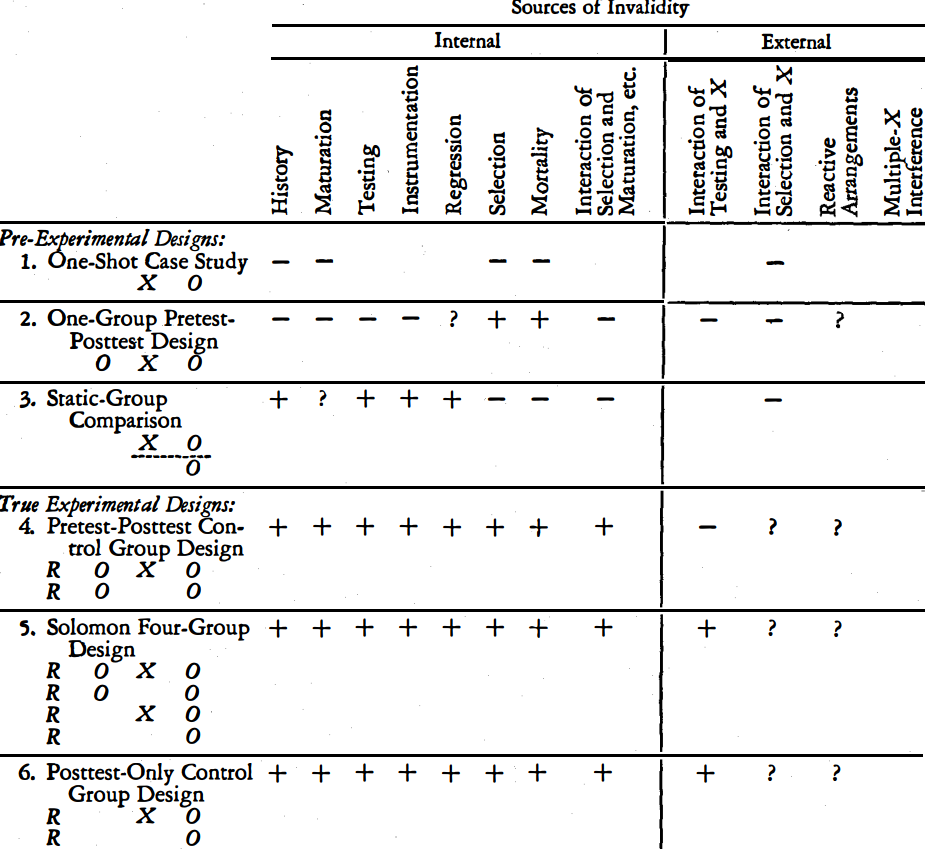
\includegraphics[width=0.65\linewidth]{img/pre-and-true-experimental-designs} \caption{pre- and true experimental designs (~\textsuperscript{\citeproc{ref-campbell1963}{5}} p.8)}\label{fig:unnamed-chunk-52}
\end{figure}

\subsection{backreference}\label{backreference}

\url{https://community.rstudio.com/t/how-to-create-a-backreference-to-place-of-citation-in-rmarkdown/84866}

\url{https://blog.csdn.net/RobertChenGuangzhi/article/details/50455429}

\url{https://latex.org/forum/viewtopic.php?t=3722}

\section{environment for definition, theorem, proof}\label{environment-for-definition-theorem-proof}

\url{https://bookdown.org/yihui/rmarkdown/bookdown-markdown.html}

\url{https://github.com/rstudio/rstudio/issues/5264}

\texttt{@howthebodyworks} Ideally, previews of such equations should also work inside a theorem, although I could survive without that.

\url{https://github.com/rstudio/rstudio/issues/8773}

\begin{theorem}[Theorem Name]
\protect\hypertarget{thm:label}{}\label{thm:label}Here is my theorem.
\end{theorem}

\begin{proof}[Proof Name]
Here is my proof.
\end{proof}

\begin{theorem}[Pythagorean theorem]
\protect\hypertarget{thm:pyth}{}\label{thm:pyth}For a right triangle, if \(c\) denotes the length of the hypotenuse
and \(a\) and \(b\) denote the lengths of the other two sides, we have

\[a^2 + \color{cyan}b^2 \overset{\ref{eq:emc}}= \color{red}{c^2} \]
\end{theorem}

\begin{definition}[Definition Name]
\protect\hypertarget{def:unnamed-chunk-54}{}\label{def:unnamed-chunk-54}Here is my definition.
\end{definition}

\hyperref[nice-label]{number and reference equations}

\eqref{eq:eqclass}

\eqref{eq:emc}

\ref{thm:pyth}

\begin{figure}
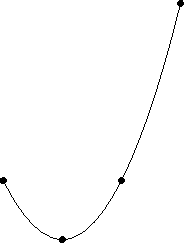
\includegraphics[width=0.25\linewidth]{202401280001-test_files/figure-latex/parabola-arc-with-points-1} \caption{parabola arc with points}\label{fig:parabola-arc-with-points}
\end{figure}

\section{slide or presentation}\label{slide-or-presentation}

\subsection{Xaringan and Infinite Moon Reader}\label{xaringan-and-infinite-moon-reader}

\url{https://rpubs.com/RW1304/xarigan-zh}

\url{https://slides.yihui.org/xaringan/\#1}

\url{https://slides.yihui.org/xaringan/zh-CN.html\#1}

\url{https://github.com/yihui/xaringan/tree/master}

\url{https://bookdown.org/yihui/rmarkdown/xaringan.html}

\subsection{ioslides}\label{ioslides}

\url{https://www.youtube.com/watch?v=gkyjTcpCITM}

\url{https://bookdown.org/yihui/rmarkdown/ioslides-presentation.html}

\url{https://stackoverflow.com/questions/63749683/how-to-set-up-theorem-environment-in-the-rmarkdown-presentation}

\begin{Shaded}
\begin{Highlighting}[]
\PreprocessorTok{{-}{-}{-}}
\FunctionTok{title}\KeywordTok{:}\AttributeTok{ }\StringTok{"Theorem demo"}
\FunctionTok{output}\KeywordTok{:}
\AttributeTok{  }\FunctionTok{ioslides\_presentation}\KeywordTok{:}
\AttributeTok{    }\FunctionTok{css}\KeywordTok{:}\AttributeTok{ style.css}
\PreprocessorTok{{-}{-}{-}}
\end{Highlighting}
\end{Shaded}

\begin{Shaded}
\begin{Highlighting}[]

\CommentTok{/* theorem environment \_ plain */}

\CommentTok{/*}
\CommentTok{.theorem \{}
\CommentTok{  display: block;}
\CommentTok{  font{-}style: italic;}
\CommentTok{  font{-}size: 24px;}
\CommentTok{  font{-}family: "Times New Roman";}
\CommentTok{  color: black;}
\CommentTok{\}}
\CommentTok{.theorem::before \{}
\CommentTok{  content: "Theorem. ";}
\CommentTok{  font{-}weight: bold;}
\CommentTok{  font{-}style: normal;}
\CommentTok{\}}
\CommentTok{.theorem[text]::before \{}
\CommentTok{  content: "Theorem (" attr(text) ") ";}
\CommentTok{\}}
\CommentTok{.theorem p \{}
\CommentTok{  display: inline;}
\CommentTok{\}}
\CommentTok{*/}

\CommentTok{/* theorem environment \_ Copenhagen style */}

\CommentTok{/*}
\CommentTok{.theorem \{}
\CommentTok{  display: block;}
\CommentTok{  font{-}style: italic;}
\CommentTok{  font{-}size: 24px;}
\CommentTok{  font{-}family: "Times New Roman";}
\CommentTok{  color: black;}
\CommentTok{  border{-}radius: 10px;}
\CommentTok{  background{-}color: rgb(222,222,231);}
\CommentTok{  box{-}shadow: 5px 10px 8px \#888888;}
\CommentTok{\}}
\CommentTok{.theorem::before \{}
\CommentTok{  content: "Theorem. ";}
\CommentTok{  font{-}weight: bold;}
\CommentTok{  font{-}style: normal;}
\CommentTok{  display: inline{-}block;}
\CommentTok{  width: {-}webkit{-}fill{-}available;}
\CommentTok{  color: white;}
\CommentTok{  border{-}radius: 10px 10px 0 0;}
\CommentTok{  padding: 10px 5px 5px 15px;}
\CommentTok{  background{-}color: rgb(38, 38, 134);}
\CommentTok{\}}
\CommentTok{.theorem p \{}
\CommentTok{  padding: 15px 15px 15px 15px;}
\CommentTok{\}}
\CommentTok{*/}
\end{Highlighting}
\end{Shaded}

\subsection{PowerPoint}\label{powerpoint}

\url{https://bookdown.org/yihui/rmarkdown/powerpoint-presentation.html}

\chapter{test2}\label{test2}

\section{verbatim}\label{verbatim}

\url{https://community.rstudio.com/t/continued-issues-with-new-verbatim-in-rstudio/139737}

\url{https://bookdown.org/yihui/rmarkdown-cookbook/verbatim-code-chunks.html}

\begin{Shaded}
\begin{Highlighting}[]


\NormalTok{\textasciigrave{}\textasciigrave{}\textasciigrave{}r}
\NormalTok{1 + 1}
\NormalTok{\textasciigrave{}\textasciigrave{}\textasciigrave{}}

\NormalTok{\textasciigrave{}\textasciigrave{}\textasciigrave{}}
\NormalTok{\#\# [1] 2}
\NormalTok{\textasciigrave{}\textasciigrave{}\textasciigrave{}}
\end{Highlighting}
\end{Shaded}

\begin{Shaded}
\begin{Highlighting}[]
\NormalTok{We can output arbitrary content **verbatim**.}


\InformationTok{\textasciigrave{}\textasciigrave{}\textasciigrave{}r}
\DecValTok{1} \SpecialCharTok{+} \DecValTok{1}
\InformationTok{\textasciigrave{}\textasciigrave{}\textasciigrave{}}

\InformationTok{\textasciigrave{}\textasciigrave{}\textasciigrave{}}
\InformationTok{\#\# [1] 2}
\InformationTok{\textasciigrave{}\textasciigrave{}\textasciigrave{}}

\NormalTok{The content can contain inline code like}
\NormalTok{78.5398163, too.}
\end{Highlighting}
\end{Shaded}

\chapter{partition}\label{partition}

\begin{align*}
 & \left\{ A_{i}\right\} _{i\in I}=\left\{ A_{i}\middle|i\in I\right\} \text{ is a partition of a set }A\\
\Leftrightarrow & \begin{cases}
\forall i\in I\left(A_{i}\ne\emptyset\right)\\
A=\bigcup\limits _{i\in I}A_{i}\\
\forall i,j\in I\left(i\ne j\Rightarrow A_{i}\cap A_{j}=\emptyset\right)
\end{cases}
\end{align*}

\url{https://proofwiki.org/wiki/Definition:Set_Partition}

\chapter{equivalence class}\label{equivalence-class}

\begin{align*}
 & C\text{ is an equivalence class of }a\text{ on }A\\
\Leftrightarrow & \left[a\right]_{\sim}=C=\left\{ x\middle|\begin{cases}
a\in A\\
x\in A\\
x\sim a\\
\sim\text{ is an equivalence relation over }A\times A=A^{2}
\end{cases}\right\} \subseteq A\ne\emptyset\\
\Leftrightarrow & \left[a\right]=\left[a\right]_{\sim}=\left\{ x\middle|\begin{cases}
a\in A\\
x\in A\\
x\sim a\\
\sim\text{ is an equivalence relation on }A
\end{cases}\right\} \subseteq A\ne\emptyset\\
\Rightarrow & \left[a\right]_{\sim}=\left\{ x\middle|x\sim a\right\} \subseteq A\ne\emptyset
\end{align*}

where the definition of \hyperref[equivalence-relation]{equivalence relation} can be found in \ref{equivalence-relation}.

\chapter{equivalence relation}\label{equivalence-relation}

\begin{CJK}{UTF8}{bsmi}等價關係 equivalence relation \label{def:equivalence-relation}
\end{CJK}
\begin{CJK}{UTF8}{bsmi}
\begin{align*}
 & R\text{ is an equivalence relation over }A\times B\\
\Leftrightarrow & \begin{cases}
R=\sim=\left\{ \left\langle x,y\right\rangle \middle|x\sim y\right\} \subseteq A\times B & \left(\text{e}\right)\text{equivalence 等價}\\
\vdots & \vdots
\end{cases}\\
\Leftrightarrow & \begin{cases}
R=\left\{ \left\langle x,y\right\rangle \middle|xRy\right\} \subseteq A\times B & \left(R\right)\text{relation}\\
\forall\left\langle x,y\right\rangle \in R\left(xRx\right) & \left(r\right)\text{reflexive}\\
\forall\left\langle x,y\right\rangle \in R\left(xRy\Rightarrow yRx\right) & \left(s\right)\text{symmetric}\\
\forall\left\langle x,y\right\rangle ,\left\langle y,z\right\rangle \in R\left(\begin{cases}
xRy\\
yRz
\end{cases}\Rightarrow xRz\right) & \left(t\right)\text{transitive}
\end{cases}\Leftrightarrow\begin{cases}
R=\left\{ \left\langle x,y\right\rangle \middle|xRy\right\} \subseteq A\times B & \text{關係}\\
\forall\left\langle x,y\right\rangle \in R\left(\left\langle x,x\right\rangle \in R\right) & \text{自反}\\
\forall\left\langle x,y\right\rangle \in R\left(\left\langle y,x\right\rangle \in R\right) & \text{對稱}\\
\forall\left\langle x,y\right\rangle ,\left\langle y,z\right\rangle \in R\left(\left\langle x,z\right\rangle \in R\right) & \text{遞移}
\end{cases}
\end{align*}
\end{CJK}

\chapter{Python}\label{python}

\section{using Python in R / RMarkdown}\label{using-python-in-r-rmarkdown}

\url{https://bookdown.org/yihui/rmarkdown/language-engines.html}

\begin{Shaded}
\begin{Highlighting}[]
\FunctionTok{names}\NormalTok{(knitr}\SpecialCharTok{::}\NormalTok{knit\_engines}\SpecialCharTok{$}\FunctionTok{get}\NormalTok{())}
\end{Highlighting}
\end{Shaded}

\begin{verbatim}
##  [1] "awk"         "bash"        "coffee"      "gawk"        "groovy"     
##  [6] "haskell"     "lein"        "mysql"       "node"        "octave"     
## [11] "perl"        "php"         "psql"        "Rscript"     "ruby"       
## [16] "sas"         "scala"       "sed"         "sh"          "stata"      
## [21] "zsh"         "asis"        "asy"         "block"       "block2"     
## [26] "bslib"       "c"           "cat"         "cc"          "comment"    
## [31] "css"         "ditaa"       "dot"         "embed"       "eviews"     
## [36] "exec"        "fortran"     "fortran95"   "go"          "highlight"  
## [41] "js"          "julia"       "python"      "R"           "Rcpp"       
## [46] "sass"        "scss"        "sql"         "stan"        "targets"    
## [51] "tikz"        "verbatim"    "theorem"     "lemma"       "corollary"  
## [56] "proposition" "conjecture"  "definition"  "example"     "exercise"   
## [61] "hypothesis"  "proof"       "remark"      "solution"
\end{verbatim}

\url{https://rstudio.github.io/reticulate/articles/python_packages.html}

\begin{Shaded}
\begin{Highlighting}[]
\NormalTok{x }\OperatorTok{=} \StringTok{\textquotesingle{}hello, python world!\textquotesingle{}}
\BuiltInTok{print}\NormalTok{(x.split(}\StringTok{\textquotesingle{} \textquotesingle{}}\NormalTok{))}
\end{Highlighting}
\end{Shaded}

\begin{verbatim}
## ['hello,', 'python', 'world!']
\end{verbatim}

\begin{Shaded}
\begin{Highlighting}[]
\FunctionTok{library}\NormalTok{(reticulate)}
\FunctionTok{virtualenv\_python}\NormalTok{()}
\end{Highlighting}
\end{Shaded}

\begin{Shaded}
\begin{Highlighting}[]
\FunctionTok{library}\NormalTok{(reticulate)}
\CommentTok{\# conda\_list()}
\end{Highlighting}
\end{Shaded}

\begin{Shaded}
\begin{Highlighting}[]
\FunctionTok{library}\NormalTok{(reticulate)}
\FunctionTok{virtualenv\_list}\NormalTok{()}
\end{Highlighting}
\end{Shaded}

\url{https://rstudio.github.io/reticulate/reference/install_python.html}

\begin{Shaded}
\begin{Highlighting}[]
\FunctionTok{library}\NormalTok{(reticulate)}
\NormalTok{version }\OtherTok{\textless{}{-}} \StringTok{"3.9.12"}
\CommentTok{\# install\_python(version)}

\DocumentationTok{\#\# create a new environment}
\CommentTok{\# virtualenv\_create("r{-}reticulate", version = version)}

\CommentTok{\# use\_virtualenv("r{-}reticulate")}

\DocumentationTok{\#\# install MatPlotLib}
\CommentTok{\# virtualenv\_install("r{-}reticulate", "matplotlib")}

\DocumentationTok{\#\# import MatPlotLib (it will be automatically discovered in "r{-}reticulate")}
\NormalTok{matplotlib }\OtherTok{\textless{}{-}} \FunctionTok{import}\NormalTok{(}\StringTok{"matplotlib"}\NormalTok{)}
\end{Highlighting}
\end{Shaded}

copy \texttt{C:\textbackslash{}Users\textbackslash{}RW\textbackslash{}AppData\textbackslash{}Local\textbackslash{}r-reticulate\textbackslash{}r-reticulate\textbackslash{}pyenv\textbackslash{}pyenv-win\textbackslash{}versions\textbackslash{}3.9.12\textbackslash{}tcl\textbackslash{}tcl8.6} and \texttt{C:\textbackslash{}Users\textbackslash{}RW\textbackslash{}AppData\textbackslash{}Local\textbackslash{}r-reticulate\textbackslash{}r-reticulate\textbackslash{}pyenv\textbackslash{}pyenv-win\textbackslash{}versions\textbackslash{}3.9.12\textbackslash{}tcl\textbackslash{}tk8.6} two folders to the folder \texttt{C:\textbackslash{}Users\textbackslash{}RW\textbackslash{}AppData\textbackslash{}Local\textbackslash{}r-reticulate\textbackslash{}r-reticulate\textbackslash{}pyenv\textbackslash{}pyenv-win\textbackslash{}versions\textbackslash{}3.9.12\textbackslash{}Lib}

\begin{Shaded}
\begin{Highlighting}[]
\CommentTok{\# library(reticulate)}
\CommentTok{\# use\_virtualenv("r{-}reticulate")}
\CommentTok{\# \# matplotlib \textless{}{-} import("matplotlib")}
\CommentTok{\# matplotlib$use("Agg", force = TRUE)}
\end{Highlighting}
\end{Shaded}

\begin{Shaded}
\begin{Highlighting}[]
\ImportTok{import}\NormalTok{ matplotlib.pyplot }\ImportTok{as}\NormalTok{ plt}
\NormalTok{plt.plot([}\DecValTok{0}\NormalTok{, }\DecValTok{2}\NormalTok{, }\DecValTok{1}\NormalTok{, }\DecValTok{4}\NormalTok{])}
\NormalTok{plt.show()}
\end{Highlighting}
\end{Shaded}

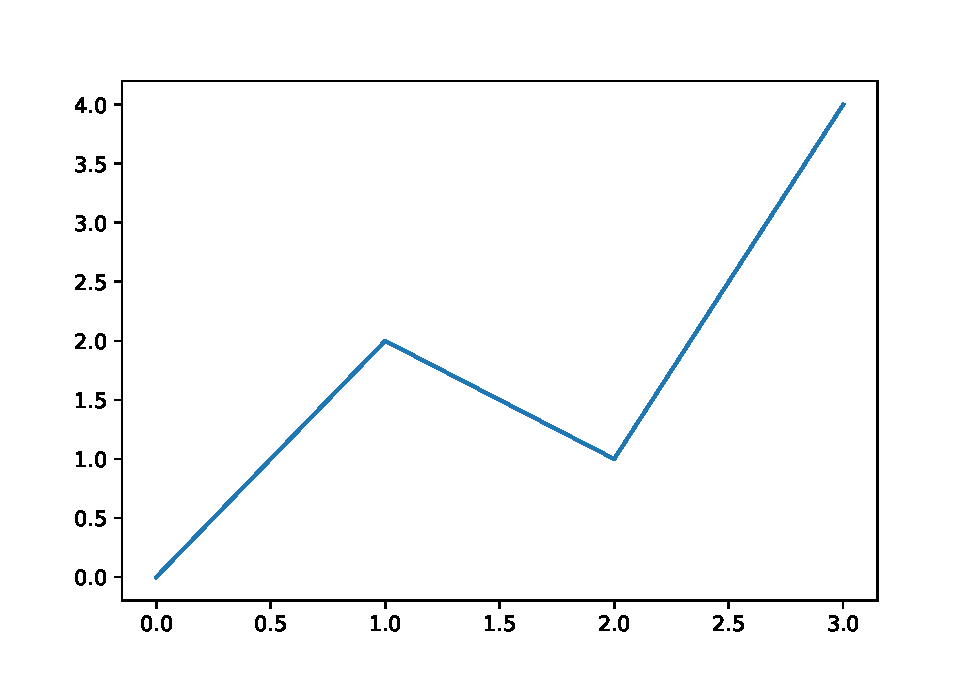
\includegraphics{202401292317-Python_files/figure-latex/unnamed-chunk-9-1.pdf}

\section{SoloLearn}\label{sololearn}

\url{https://www.sololearn.com/}

\url{https://www.sololearn.com/en/learn/courses/python-intermediate}

\section{list comprehension}\label{list-comprehension}

\url{https://www.sololearn.com/en/learn/courses/python-intermediate/lesson/1188906590?p=1}

\begin{cols}

\begin{col}{0.45\textwidth}

\begin{Shaded}
\begin{Highlighting}[]
\NormalTok{cubes }\OperatorTok{=}\NormalTok{ [i}\OperatorTok{**}\DecValTok{3} \ControlFlowTok{for}\NormalTok{ i }\KeywordTok{in} \BuiltInTok{range}\NormalTok{(}\DecValTok{5}\NormalTok{)]}

\BuiltInTok{print}\NormalTok{(cubes)}
\end{Highlighting}
\end{Shaded}

\end{col}

\begin{col}{0.10\textwidth}
~

\end{col}

\begin{col}{0.45\textwidth}

\begin{verbatim}
## [0, 1, 8, 27, 64]
\end{verbatim}

\end{col}

\end{cols}

\section{functional programming}\label{functional-programming}

\begin{itemize}
\tightlist
\item
  pure function
\item
  lambda
\item
  map
\item
  filter
\item
  generator
\item
  decorator
\item
  recursion
\item
  *args
\item
  **kwargs
\end{itemize}

\section{object-oriented programming = OOP}\label{object-oriented-programming-oop}

\begin{itemize}
\tightlist
\item
  class
\item
  inheritance
\item
  magic method
\item
  operator overloading
\item
  data hiding
\item
  static method
\item
  property
\end{itemize}

\chapter{TikZ}\label{tikz}

\begin{itemize}
\tightlist
\item
  Ti\(k\)Z

  \begin{itemize}
  \tightlist
  \item
    \hyperref[pgfplots]{PGFplots}\textsuperscript{{[}\ref{pgfplots}{]}}
  \item
    tikzplotlib\textsuperscript{{[}\ref{tikzplotlib}{]}}: \hyperref[python]{Python}\textsuperscript{{[}\ref{python}{]}} matplotlib\textsuperscript{{[}\ref{matplotlib}{]}} export to \hyperref[tikz]{TikZ}\textsuperscript{{[}\ref{tikz}{]}} .tex
  \end{itemize}
\end{itemize}

multi-column \ref{multi-column}

\begin{Shaded}
\begin{Highlighting}[]
\NormalTok{knitr}\SpecialCharTok{::}\NormalTok{opts\_chunk}\SpecialCharTok{$}\FunctionTok{set}\NormalTok{(}\AttributeTok{fig.pos =} \StringTok{"H"}\NormalTok{, }\AttributeTok{out.extra =} \StringTok{""}\NormalTok{)}
\end{Highlighting}
\end{Shaded}

\url{https://bookdown.org/yihui/rmarkdown-cookbook/html-scroll.html}

\begin{cols}

\begin{col}{0.45\textwidth}

\begin{Shaded}
\begin{Highlighting}[]
\KeywordTok{\textbackslash{}begin}\NormalTok{\{}\ExtensionTok{tikzpicture}\NormalTok{\}}
  \FunctionTok{\textbackslash{}draw}\NormalTok{ ({-}1,1){-}{-}(0,0){-}{-}(1,2);}
\KeywordTok{\textbackslash{}end}\NormalTok{\{}\ExtensionTok{tikzpicture}\NormalTok{\}}
\end{Highlighting}
\end{Shaded}

\end{col}

\begin{col}{0.10\textwidth}
~

\end{col}

\begin{col}{0.45\textwidth}

\begin{figure}[H]
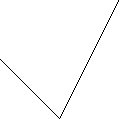
\includegraphics{202401311000-TikZ_files/figure-latex/unnamed-chunk-4-1} \end{figure}

\end{col}

\end{cols}

How to speed up bookdown generation?

\url{https://stackoverflow.com/questions/56541371/how-to-speed-up-bookdown-generation}

TikZ and PGFplots

What's the relation between packages PGFplots and TikZ?

\url{https://tex.stackexchange.com/questions/285925/whats-the-relation-between-packages-pgfplots-and-tikz}

\url{https://www.youtube.com/watch?v=bQugbYq0BVA}

\url{https://www.youtube.com/watch?v=ft4Kg9emK1k&list=PLg5nrpKdkk2DWcg3scb75AknF7DJXs8lk&index=18}

\begin{cols}

\begin{col}{0.45\textwidth}

\begin{Shaded}
\begin{Highlighting}[]
\KeywordTok{\textbackslash{}begin}\NormalTok{\{}\ExtensionTok{tikzpicture}\NormalTok{\}}
  \FunctionTok{\textbackslash{}def\textbackslash{}a}\NormalTok{\{1.5\} }\CommentTok{\% amplitude}
  \FunctionTok{\textbackslash{}def\textbackslash{}b}\NormalTok{\{2\}   }\CommentTok{\% frequency}
  \FunctionTok{\textbackslash{}draw}\NormalTok{[{-}\textgreater{}] ({-}0.2,0){-}{-}(4.2,0) node[right, font=}\FunctionTok{\textbackslash{}small}\NormalTok{] \{}\SpecialStringTok{$x$}\NormalTok{\};}
  \FunctionTok{\textbackslash{}draw}\NormalTok{[{-}\textgreater{}] (0,{-}4){-}{-}(0,0.5) node[above] \{}\SpecialStringTok{$y$}\NormalTok{\};}
  \FunctionTok{\textbackslash{}draw}\NormalTok{[domain=0:4,smooth,variable=}\FunctionTok{\textbackslash{}t}\NormalTok{,blue,thick] }
\NormalTok{    plot (\{}\FunctionTok{\textbackslash{}a}\NormalTok{ * (}\FunctionTok{\textbackslash{}b*\textbackslash{}t}\NormalTok{ {-} sin(deg(}\FunctionTok{\textbackslash{}b*\textbackslash{}t}\NormalTok{)))\},\{{-}}\FunctionTok{\textbackslash{}a}\NormalTok{ * (1 {-} cos(deg(}\FunctionTok{\textbackslash{}b*\textbackslash{}t}\NormalTok{)))\});}
  \CommentTok{\% \textbackslash{}node[above] at (2, 0.5) \{Brachistochrone Curve\};}
  \FunctionTok{\textbackslash{}node}\NormalTok{[above, font=}\FunctionTok{\textbackslash{}footnotesize}\NormalTok{] at (2, 1) \{Brachistochrone Curve\};}
  \FunctionTok{\textbackslash{}node}\NormalTok{[above, font=}\FunctionTok{\textbackslash{}footnotesize}\NormalTok{] at (2, 0) \{}\SpecialStringTok{$}\KeywordTok{\textbackslash{}begin}\NormalTok{\{}\ExtensionTok{aligned}\NormalTok{\}}
\SpecialStringTok{\& x=r(t{-}}\SpecialCharTok{\textbackslash{}sin}\SpecialStringTok{ t) }\SpecialCharTok{\textbackslash{}\textbackslash{}}
\SpecialStringTok{\& y=r(1{-}}\SpecialCharTok{\textbackslash{}cos}\SpecialStringTok{ t)}
\KeywordTok{\textbackslash{}end}\NormalTok{\{}\ExtensionTok{aligned}\NormalTok{\}}\SpecialStringTok{$}\NormalTok{\};}
\KeywordTok{\textbackslash{}end}\NormalTok{\{}\ExtensionTok{tikzpicture}\NormalTok{\}}
\end{Highlighting}
\end{Shaded}

\end{col}

\begin{col}{0.10\textwidth}
~

\end{col}

\begin{col}{0.45\textwidth}

\begin{figure}[H]
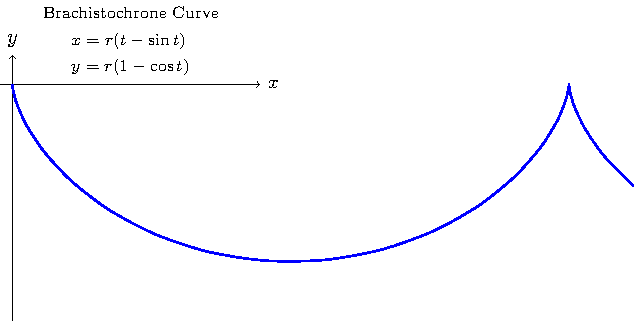
\includegraphics{202401311000-TikZ_files/figure-latex/unnamed-chunk-6-1} \caption{Brachistochrone Curve}\label{fig:unnamed-chunk-6}
\end{figure}

\end{col}

\end{cols}

\begin{figure}[H]
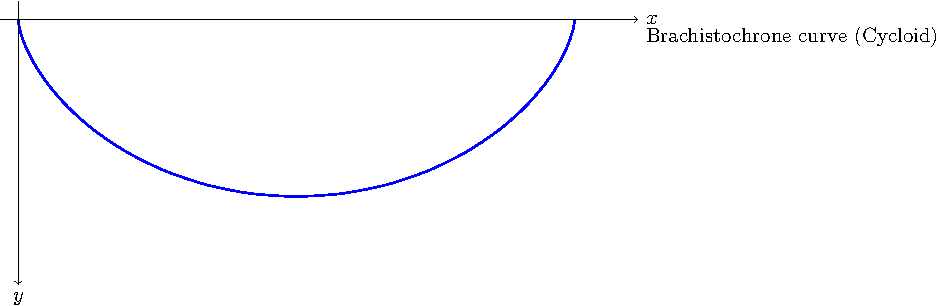
\includegraphics[width=0.9\linewidth,]{202401311000-TikZ_files/figure-latex/unnamed-chunk-7-1} \caption{Brachistochrone Curve}\label{fig:unnamed-chunk-7}
\end{figure}

\section{2D}\label{d}

\url{https://zhuanlan.zhihu.com/p/127155579?utm_psn=1741479950987960320}

\begin{Shaded}
\begin{Highlighting}[]
\KeywordTok{\textbackslash{}begin}\NormalTok{\{}\ExtensionTok{tikzpicture}\NormalTok{\}}
  \FunctionTok{\textbackslash{}draw}\NormalTok{ ({-}1,1){-}{-}(0,0){-}{-}(1,2);}
\KeywordTok{\textbackslash{}end}\NormalTok{\{}\ExtensionTok{tikzpicture}\NormalTok{\}}
\end{Highlighting}
\end{Shaded}

\begin{center}\rule{0.5\linewidth}{0.5pt}\end{center}

\begin{cols}

\begin{col}{0.45\textwidth}

\begin{Shaded}
\begin{Highlighting}[]
\KeywordTok{\textbackslash{}begin}\NormalTok{\{}\ExtensionTok{tikzpicture}\NormalTok{\}}
  \FunctionTok{\textbackslash{}draw}\NormalTok{ ({-}1,1){-}{-}(0,0){-}{-}(1,2);}
\KeywordTok{\textbackslash{}end}\NormalTok{\{}\ExtensionTok{tikzpicture}\NormalTok{\}}
\end{Highlighting}
\end{Shaded}

\end{col}

\begin{col}{0.10\textwidth}
~

\end{col}

\begin{col}{0.45\textwidth}
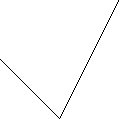
\includegraphics{202401311000-TikZ_files/figure-latex/unnamed-chunk-10-1}

\end{col}

\end{cols}

\begin{center}\rule{0.5\linewidth}{0.5pt}\end{center}

\begin{cols}

\begin{col}{0.45\textwidth}

\texttt{out.width=if\ (knitr:::is\_html\_output())\ \textquotesingle{}20\%\textquotesingle{}}

\begin{Shaded}
\begin{Highlighting}[]
\KeywordTok{\textbackslash{}begin}\NormalTok{\{}\ExtensionTok{tikzpicture}\NormalTok{\}}
  \FunctionTok{\textbackslash{}draw}\NormalTok{ ({-}1,1){-}{-}(0,0){-}{-}(1,2);}
\KeywordTok{\textbackslash{}end}\NormalTok{\{}\ExtensionTok{tikzpicture}\NormalTok{\}}
\end{Highlighting}
\end{Shaded}

\end{col}

\begin{col}{0.10\textwidth}
~

\end{col}

\begin{col}{0.45\textwidth}
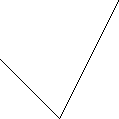
\includegraphics{202401311000-TikZ_files/figure-latex/unnamed-chunk-12-1}

\end{col}

\end{cols}

\begin{center}\rule{0.5\linewidth}{0.5pt}\end{center}

\begin{cols}

\begin{col}{0.45\textwidth}

\begin{Shaded}
\begin{Highlighting}[]
\KeywordTok{\textbackslash{}begin}\NormalTok{\{}\ExtensionTok{tikzpicture}\NormalTok{\}}
  \FunctionTok{\textbackslash{}draw}\NormalTok{[rounded corners] ({-}1,1){-}{-}(0,0){-}{-}(1,2){-}{-}({-}1,1);}
\KeywordTok{\textbackslash{}end}\NormalTok{\{}\ExtensionTok{tikzpicture}\NormalTok{\}}
\end{Highlighting}
\end{Shaded}

\end{col}

\begin{col}{0.10\textwidth}
~

\end{col}

\begin{col}{0.45\textwidth}

\begin{figure}[H]
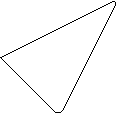
\includegraphics{202401311000-TikZ_files/figure-latex/unnamed-chunk-14-1} \caption{rounded corner pseudo-closed triangle}\label{fig:unnamed-chunk-14}
\end{figure}

\end{col}

\end{cols}

\begin{center}\rule{0.5\linewidth}{0.5pt}\end{center}

\begin{cols}

\begin{col}{0.45\textwidth}

\begin{Shaded}
\begin{Highlighting}[]
\KeywordTok{\textbackslash{}begin}\NormalTok{\{}\ExtensionTok{tikzpicture}\NormalTok{\}}
  \FunctionTok{\textbackslash{}draw}\NormalTok{[rounded corners] ({-}1,1){-}{-}(0,0){-}{-}(1,2){-}{-}cycle;}
\KeywordTok{\textbackslash{}end}\NormalTok{\{}\ExtensionTok{tikzpicture}\NormalTok{\}}
\end{Highlighting}
\end{Shaded}

\end{col}

\begin{col}{0.10\textwidth}
~

\end{col}

\begin{col}{0.45\textwidth}

\begin{figure}[H]
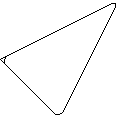
\includegraphics{202401311000-TikZ_files/figure-latex/unnamed-chunk-16-1} \caption{rounded corner triangle}\label{fig:unnamed-chunk-16}
\end{figure}

\end{col}

\end{cols}

\begin{center}\rule{0.5\linewidth}{0.5pt}\end{center}

\begin{cols}

\begin{col}{0.45\textwidth}

\begin{Shaded}
\begin{Highlighting}[]
\KeywordTok{\textbackslash{}begin}\NormalTok{\{}\ExtensionTok{tikzpicture}\NormalTok{\}}
  \FunctionTok{\textbackslash{}draw}\NormalTok{[rounded corners] ({-}1,1){-}{-}(0,0){-}{-}(1,2){-}{-}cycle;}
  \FunctionTok{\textbackslash{}draw}\NormalTok{[rounded corners] ({-}1,1){-}{-}(0,0){-}{-}(1,2){-}{-}({-}1,1);}
\KeywordTok{\textbackslash{}end}\NormalTok{\{}\ExtensionTok{tikzpicture}\NormalTok{\}}
\end{Highlighting}
\end{Shaded}

\end{col}

\begin{col}{0.10\textwidth}
~

\end{col}

\begin{col}{0.45\textwidth}

\begin{figure}[H]
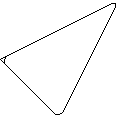
\includegraphics{202401311000-TikZ_files/figure-latex/unnamed-chunk-18-1} \caption{triangle vs. pseudo-closed triangle}\label{fig:unnamed-chunk-18}
\end{figure}

\end{col}

\end{cols}

\begin{center}\rule{0.5\linewidth}{0.5pt}\end{center}

\begin{cols}

\begin{col}{0.45\textwidth}

\begin{Shaded}
\begin{Highlighting}[]
\KeywordTok{\textbackslash{}begin}\NormalTok{\{}\ExtensionTok{tikzpicture}\NormalTok{\}}
  \FunctionTok{\textbackslash{}draw}\NormalTok{ (0,0) rectangle (4,2);}
\KeywordTok{\textbackslash{}end}\NormalTok{\{}\ExtensionTok{tikzpicture}\NormalTok{\}}
\end{Highlighting}
\end{Shaded}

\end{col}

\begin{col}{0.10\textwidth}
~

\end{col}

\begin{col}{0.45\textwidth}

\begin{figure}[H]

\includegraphics{202401311000-TikZ_files/figure-latex/unnamed-chunk-20-1} \caption{rectangle}\label{fig:unnamed-chunk-20}
\end{figure}

\end{col}

\end{cols}

\begin{center}\rule{0.5\linewidth}{0.5pt}\end{center}

\begin{cols}

\begin{col}{0.45\textwidth}

\begin{Shaded}
\begin{Highlighting}[]
\KeywordTok{\textbackslash{}begin}\NormalTok{\{}\ExtensionTok{tikzpicture}\NormalTok{\}}
  \FunctionTok{\textbackslash{}draw}\NormalTok{ (0,0) rectangle (2,2);}
\KeywordTok{\textbackslash{}end}\NormalTok{\{}\ExtensionTok{tikzpicture}\NormalTok{\}}
\end{Highlighting}
\end{Shaded}

\end{col}

\begin{col}{0.10\textwidth}
~

\end{col}

\begin{col}{0.45\textwidth}

\begin{figure}[H]

\includegraphics{202401311000-TikZ_files/figure-latex/unnamed-chunk-22-1} \caption{square}\label{fig:unnamed-chunk-22}
\end{figure}

\end{col}

\end{cols}

\begin{center}\rule{0.5\linewidth}{0.5pt}\end{center}

\begin{cols}

\begin{col}{0.45\textwidth}

\begin{Shaded}
\begin{Highlighting}[]
\KeywordTok{\textbackslash{}begin}\NormalTok{\{}\ExtensionTok{tikzpicture}\NormalTok{\}}
  \FunctionTok{\textbackslash{}draw}\NormalTok{ (0,0) circle (1);}
\KeywordTok{\textbackslash{}end}\NormalTok{\{}\ExtensionTok{tikzpicture}\NormalTok{\}}
\end{Highlighting}
\end{Shaded}

\end{col}

\begin{col}{0.10\textwidth}
~

\end{col}

\begin{col}{0.45\textwidth}

\begin{figure}[H]
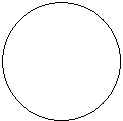
\includegraphics{202401311000-TikZ_files/figure-latex/unnamed-chunk-24-1} \caption{circle}\label{fig:unnamed-chunk-24}
\end{figure}

\end{col}

\end{cols}

\begin{center}\rule{0.5\linewidth}{0.5pt}\end{center}

\begin{cols}

\begin{col}{0.45\textwidth}

\begin{Shaded}
\begin{Highlighting}[]
\KeywordTok{\textbackslash{}begin}\NormalTok{\{}\ExtensionTok{tikzpicture}\NormalTok{\}}
  \FunctionTok{\textbackslash{}draw}\NormalTok{ (0,0) circle (1);}
  \FunctionTok{\textbackslash{}draw}\NormalTok{ (0,0) rectangle (2,2);}
\KeywordTok{\textbackslash{}end}\NormalTok{\{}\ExtensionTok{tikzpicture}\NormalTok{\}}
\end{Highlighting}
\end{Shaded}

\end{col}

\begin{col}{0.10\textwidth}
~

\end{col}

\begin{col}{0.45\textwidth}

\begin{figure}[H]
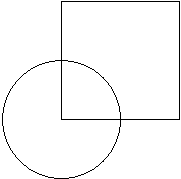
\includegraphics{202401311000-TikZ_files/figure-latex/unnamed-chunk-26-1} \caption{circle and square}\label{fig:unnamed-chunk-26}
\end{figure}

\end{col}

\end{cols}

\begin{center}\rule{0.5\linewidth}{0.5pt}\end{center}

\begin{cols}

\begin{col}{0.45\textwidth}

\begin{Shaded}
\begin{Highlighting}[]
\KeywordTok{\textbackslash{}begin}\NormalTok{\{}\ExtensionTok{tikzpicture}\NormalTok{\}}
  \FunctionTok{\textbackslash{}draw}\NormalTok{ (1,1) ellipse (2 and 1);}
\KeywordTok{\textbackslash{}end}\NormalTok{\{}\ExtensionTok{tikzpicture}\NormalTok{\}}
\end{Highlighting}
\end{Shaded}

\end{col}

\begin{col}{0.10\textwidth}
~

\end{col}

\begin{col}{0.45\textwidth}

\begin{figure}[H]
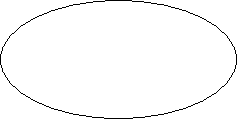
\includegraphics{202401311000-TikZ_files/figure-latex/unnamed-chunk-28-1} \caption{ellipse}\label{fig:unnamed-chunk-28}
\end{figure}

\end{col}

\end{cols}

\begin{center}\rule{0.5\linewidth}{0.5pt}\end{center}

\begin{cols}

\begin{col}{0.45\textwidth}

\begin{Shaded}
\begin{Highlighting}[]
\KeywordTok{\textbackslash{}begin}\NormalTok{\{}\ExtensionTok{tikzpicture}\NormalTok{\}}
  \FunctionTok{\textbackslash{}draw}\NormalTok{ (1 ,1) arc (0:270:1);}
  \FunctionTok{\textbackslash{}draw}\NormalTok{ (6 ,1) arc (0:270:2 and 1);}
\KeywordTok{\textbackslash{}end}\NormalTok{\{}\ExtensionTok{tikzpicture}\NormalTok{\}}
\end{Highlighting}
\end{Shaded}

\end{col}

\begin{col}{0.10\textwidth}
~

\end{col}

\begin{col}{0.45\textwidth}

\begin{figure}[H]
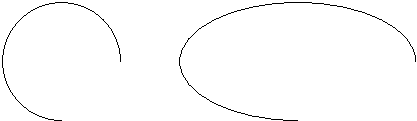
\includegraphics{202401311000-TikZ_files/figure-latex/unnamed-chunk-30-1} \caption{circle and ellipse arcs}\label{fig:unnamed-chunk-30}
\end{figure}

\end{col}

\end{cols}

\begin{center}\rule{0.5\linewidth}{0.5pt}\end{center}

\begin{cols}

\begin{col}{0.45\textwidth}

\begin{Shaded}
\begin{Highlighting}[]
\KeywordTok{\textbackslash{}begin}\NormalTok{\{}\ExtensionTok{tikzpicture}\NormalTok{\}}
  \FunctionTok{\textbackslash{}draw}\NormalTok{ ({-}1,1) parabola bend (0,0) (2,4);}
\KeywordTok{\textbackslash{}end}\NormalTok{\{}\ExtensionTok{tikzpicture}\NormalTok{\}}
\end{Highlighting}
\end{Shaded}

\end{col}

\begin{col}{0.10\textwidth}
~

\end{col}

\begin{col}{0.45\textwidth}

\begin{figure}[H]

\includegraphics{202401311000-TikZ_files/figure-latex/unnamed-chunk-32-1} \caption{parabola arc}\label{fig:unnamed-chunk-32}
\end{figure}

\end{col}

\end{cols}

\begin{center}\rule{0.5\linewidth}{0.5pt}\end{center}

\begin{cols}

\begin{col}{0.45\textwidth}

\begin{Shaded}
\begin{Highlighting}[]
\KeywordTok{\textbackslash{}begin}\NormalTok{\{}\ExtensionTok{tikzpicture}\NormalTok{\}}
  \FunctionTok{\textbackslash{}draw}\NormalTok{ ({-}1,1) parabola bend (0,0) (2,4);}
  \FunctionTok{\textbackslash{}filldraw}
\NormalTok{    ({-}1,1) circle (.05)}
\NormalTok{    ( 0,0) circle (.05)}
\NormalTok{    ( 1,1) circle (.05)}
\NormalTok{    ( 2,4) circle (.05);}
\KeywordTok{\textbackslash{}end}\NormalTok{\{}\ExtensionTok{tikzpicture}\NormalTok{\}}
\end{Highlighting}
\end{Shaded}

\end{col}

\begin{col}{0.10\textwidth}
~

\end{col}

\begin{col}{0.45\textwidth}

\begin{figure}[H]
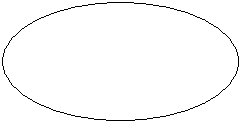
\includegraphics{202401311000-TikZ_files/figure-latex/unnamed-chunk-34-1} \caption{parabola arc with points}\label{fig:unnamed-chunk-34}
\end{figure}

\end{col}

\end{cols}

\begin{center}\rule{0.5\linewidth}{0.5pt}\end{center}

\begin{cols}

\begin{col}{0.45\textwidth}

\begin{Shaded}
\begin{Highlighting}[]
\KeywordTok{\textbackslash{}begin}\NormalTok{\{}\ExtensionTok{tikzpicture}\NormalTok{\}}
  \FunctionTok{\textbackslash{}draw}\NormalTok{[step=20pt] (0,0) grid (3,2);}
  \FunctionTok{\textbackslash{}draw}\NormalTok{[help lines ,step=20pt] (4,0) grid (7,2);}
\KeywordTok{\textbackslash{}end}\NormalTok{\{}\ExtensionTok{tikzpicture}\NormalTok{\}}
\end{Highlighting}
\end{Shaded}

\end{col}

\begin{col}{0.10\textwidth}
~

\end{col}

\begin{col}{0.45\textwidth}

\begin{figure}[H]

\includegraphics{202401311000-TikZ_files/figure-latex/unnamed-chunk-36-1} \caption{grid and help lines}\label{fig:unnamed-chunk-36}
\end{figure}

\end{col}

\end{cols}

\begin{center}\rule{0.5\linewidth}{0.5pt}\end{center}

\begin{cols}

\begin{col}{0.45\textwidth}

\begin{Shaded}
\begin{Highlighting}[]
\KeywordTok{\textbackslash{}begin}\NormalTok{\{}\ExtensionTok{tikzpicture}\NormalTok{\}[scale=0.25]}
  \FunctionTok{\textbackslash{}draw}\NormalTok{[{-}\textgreater{}] (0,0){-}{-}(9,0);}
  \FunctionTok{\textbackslash{}draw}\NormalTok{[\textless{}{-}] (0,1){-}{-}(9,1);}
  \FunctionTok{\textbackslash{}draw}\NormalTok{[\textless{}{-}\textgreater{}] (0,2){-}{-}(9,2);}
  \FunctionTok{\textbackslash{}draw}\NormalTok{[\textgreater{}{-}\textgreater{}\textgreater{}] (0,3){-}{-}(9,3);}
  \FunctionTok{\textbackslash{}draw}\NormalTok{[|\textless{}{-}\textgreater{}|] (0,4){-}{-}(9,4);}
\KeywordTok{\textbackslash{}end}\NormalTok{\{}\ExtensionTok{tikzpicture}\NormalTok{\}}
\end{Highlighting}
\end{Shaded}

\end{col}

\begin{col}{0.10\textwidth}
~

\end{col}

\begin{col}{0.45\textwidth}

\begin{figure}[H]
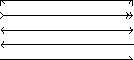
\includegraphics{202401311000-TikZ_files/figure-latex/unnamed-chunk-38-1} \caption{arrows}\label{fig:unnamed-chunk-38}
\end{figure}

\end{col}

\end{cols}

\begin{center}\rule{0.5\linewidth}{0.5pt}\end{center}

\begin{cols}

\begin{col}{0.45\textwidth}

\begin{Shaded}
\begin{Highlighting}[]
\KeywordTok{\textbackslash{}begin}\NormalTok{\{}\ExtensionTok{tikzpicture}\NormalTok{\}}
  \FunctionTok{\textbackslash{}draw}\NormalTok{[line width =2pt] (0,6){-}{-}(9,6); }
  \FunctionTok{\textbackslash{}draw}\NormalTok{[dotted]          (0,5){-}{-}(9,5); }
  \FunctionTok{\textbackslash{}draw}\NormalTok{[densely dotted]  (0,4){-}{-}(9,4); }
  \FunctionTok{\textbackslash{}draw}\NormalTok{[loosely dotted]  (0,3){-}{-}(9,3); }
  \FunctionTok{\textbackslash{}draw}\NormalTok{[dashed]          (0,2){-}{-}(9,2); }
  \FunctionTok{\textbackslash{}draw}\NormalTok{[densely dashed]  (0,1){-}{-}(9,1); }
  \FunctionTok{\textbackslash{}draw}\NormalTok{[loosely dashed]  (0,0){-}{-}(9,0);}
\KeywordTok{\textbackslash{}end}\NormalTok{\{}\ExtensionTok{tikzpicture}\NormalTok{\}}
\end{Highlighting}
\end{Shaded}

\end{col}

\begin{col}{0.10\textwidth}
~

\end{col}

\begin{col}{0.45\textwidth}

\begin{figure}[H]
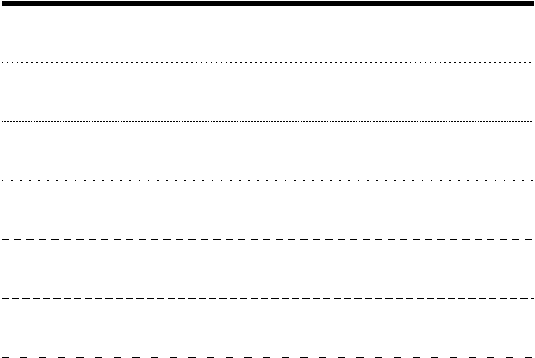
\includegraphics{202401311000-TikZ_files/figure-latex/unnamed-chunk-40-1} \caption{lines}\label{fig:unnamed-chunk-40}
\end{figure}

\end{col}

\end{cols}

\begin{center}\rule{0.5\linewidth}{0.5pt}\end{center}

\begin{cols}

\begin{col}{0.45\textwidth}

\begin{Shaded}
\begin{Highlighting}[]
\KeywordTok{\textbackslash{}begin}\NormalTok{\{}\ExtensionTok{tikzpicture}\NormalTok{\}[dline/.style=\{color= blue, line width=2pt\}]}
  \FunctionTok{\textbackslash{}draw}\NormalTok{[dline] (0,0){-}{-}(9,0); }
\KeywordTok{\textbackslash{}end}\NormalTok{\{}\ExtensionTok{tikzpicture}\NormalTok{\}}
\end{Highlighting}
\end{Shaded}

\end{col}

\begin{col}{0.10\textwidth}
~

\end{col}

\begin{col}{0.45\textwidth}

\begin{figure}[H]

\includegraphics{202401311000-TikZ_files/figure-latex/unnamed-chunk-42-1} \caption{head styling}\label{fig:unnamed-chunk-42}
\end{figure}

\end{col}

\end{cols}

\begin{center}\rule{0.5\linewidth}{0.5pt}\end{center}

\begin{cols}

\begin{col}{0.45\textwidth}

\begin{Shaded}
\begin{Highlighting}[]
\KeywordTok{\textbackslash{}begin}\NormalTok{\{}\ExtensionTok{tikzpicture}\NormalTok{\}}
  \FunctionTok{\textbackslash{}draw}\NormalTok{ (0,0) rectangle (2,2);}
  \FunctionTok{\textbackslash{}draw}\NormalTok{[shift=\{( 3, 0)\}] (0,0) rectangle (2,2);}
  \FunctionTok{\textbackslash{}draw}\NormalTok{[shift=\{( 0, 3)\}] (0,0) rectangle (2,2);}
  \FunctionTok{\textbackslash{}draw}\NormalTok{[shift=\{( 0,{-}3)\}] (0,0) rectangle (2,2);}
  \FunctionTok{\textbackslash{}draw}\NormalTok{[shift=\{({-}3, 0)\}] (0,0) rectangle (2,2);}
  \FunctionTok{\textbackslash{}draw}\NormalTok{[shift=\{( 3, 3)\}] (0,0) rectangle (2,2);}
  \FunctionTok{\textbackslash{}draw}\NormalTok{[shift=\{({-}3, 3)\}] (0,0) rectangle (2,2);}
  \FunctionTok{\textbackslash{}draw}\NormalTok{[shift=\{( 3,{-}3)\}] (0,0) rectangle (2,2);}
  \FunctionTok{\textbackslash{}draw}\NormalTok{[shift=\{({-}3,{-}3)\}] (0,0) rectangle (2,2);}
\KeywordTok{\textbackslash{}end}\NormalTok{\{}\ExtensionTok{tikzpicture}\NormalTok{\}}
\end{Highlighting}
\end{Shaded}

\end{col}

\begin{col}{0.10\textwidth}
~

\end{col}

\begin{col}{0.45\textwidth}

\begin{figure}[H]

\includegraphics{202401311000-TikZ_files/figure-latex/unnamed-chunk-44-1} \caption{transform: shift}\label{fig:unnamed-chunk-44}
\end{figure}

\end{col}

\end{cols}

\begin{center}\rule{0.5\linewidth}{0.5pt}\end{center}

\begin{cols}

\begin{col}{0.45\textwidth}

\begin{Shaded}
\begin{Highlighting}[]
\KeywordTok{\textbackslash{}begin}\NormalTok{\{}\ExtensionTok{tikzpicture}\NormalTok{\}}
  \FunctionTok{\textbackslash{}draw}\NormalTok{ (0,0) rectangle (2,2);}
  \FunctionTok{\textbackslash{}draw}\NormalTok{[xshift= 100pt] (0,0) rectangle (2,2);}
  \FunctionTok{\textbackslash{}draw}\NormalTok{[xshift={-}100pt] (0,0) rectangle (2,2);}
  \FunctionTok{\textbackslash{}draw}\NormalTok{[yshift= 100pt] (0,0) rectangle (2,2);}
  \FunctionTok{\textbackslash{}draw}\NormalTok{[yshift={-}100pt] (0,0) rectangle (2,2);}
\KeywordTok{\textbackslash{}end}\NormalTok{\{}\ExtensionTok{tikzpicture}\NormalTok{\}}
\end{Highlighting}
\end{Shaded}

\end{col}

\begin{col}{0.10\textwidth}
~

\end{col}

\begin{col}{0.45\textwidth}

\begin{figure}[H]

\includegraphics{202401311000-TikZ_files/figure-latex/unnamed-chunk-46-1} \caption{transform: shift x, y}\label{fig:unnamed-chunk-46}
\end{figure}

\end{col}

\end{cols}

\begin{center}\rule{0.5\linewidth}{0.5pt}\end{center}

\begin{cols}

\begin{col}{0.45\textwidth}

\begin{Shaded}
\begin{Highlighting}[]
\KeywordTok{\textbackslash{}begin}\NormalTok{\{}\ExtensionTok{tikzpicture}\NormalTok{\}}
  \FunctionTok{\textbackslash{}draw}\NormalTok{ (0,0) rectangle (2,2);}
  \FunctionTok{\textbackslash{}draw}\NormalTok{[xshift= 100pt, xscale=1.5] (0,0) rectangle (2,2);}
  \FunctionTok{\textbackslash{}draw}\NormalTok{[yshift= 100pt, xscale=0.5] (0,0) rectangle (2,2);}
  \FunctionTok{\textbackslash{}draw}\NormalTok{[xshift={-}100pt, yscale=1.5] (0,0) rectangle (2,2);}
  \FunctionTok{\textbackslash{}draw}\NormalTok{[yshift={-}100pt, yscale=0.5] (0,0) rectangle (2,2);}
\KeywordTok{\textbackslash{}end}\NormalTok{\{}\ExtensionTok{tikzpicture}\NormalTok{\}}
\end{Highlighting}
\end{Shaded}

\end{col}

\begin{col}{0.10\textwidth}
~

\end{col}

\begin{col}{0.45\textwidth}

\begin{figure}[H]
\includegraphics{202401311000-TikZ_files/figure-latex/unnamed-chunk-48-1} \caption{transform: scale x, y}\label{fig:unnamed-chunk-48}
\end{figure}

\end{col}

\end{cols}

\begin{center}\rule{0.5\linewidth}{0.5pt}\end{center}

\begin{cols}

\begin{col}{0.45\textwidth}

\begin{Shaded}
\begin{Highlighting}[]
\KeywordTok{\textbackslash{}begin}\NormalTok{\{}\ExtensionTok{tikzpicture}\NormalTok{\}}
  \FunctionTok{\textbackslash{}draw}\NormalTok{ (0,0) rectangle (2,2);}
  \FunctionTok{\textbackslash{}draw}\NormalTok{[xshift= 100pt, xscale=1.5] (0,0) rectangle (2,2);}
  \FunctionTok{\textbackslash{}draw}\NormalTok{[yshift= 100pt, yscale=1.5] (0,0) rectangle (2,2);}
  \FunctionTok{\textbackslash{}draw}\NormalTok{[xshift={-}100pt, xscale=0.5] (0,0) rectangle (2,2);}
  \FunctionTok{\textbackslash{}draw}\NormalTok{[yshift={-}100pt, yscale=0.5] (0,0) rectangle (2,2);}
\KeywordTok{\textbackslash{}end}\NormalTok{\{}\ExtensionTok{tikzpicture}\NormalTok{\}}
\end{Highlighting}
\end{Shaded}

\end{col}

\begin{col}{0.10\textwidth}
~

\end{col}

\begin{col}{0.45\textwidth}

\begin{figure}[H]
\includegraphics{202401311000-TikZ_files/figure-latex/unnamed-chunk-50-1} \caption{transform: scale}\label{fig:unnamed-chunk-50}
\end{figure}

\end{col}

\end{cols}

\begin{center}\rule{0.5\linewidth}{0.5pt}\end{center}

\begin{cols}

\begin{col}{0.45\textwidth}

\begin{Shaded}
\begin{Highlighting}[]
\KeywordTok{\textbackslash{}begin}\NormalTok{\{}\ExtensionTok{tikzpicture}\NormalTok{\}}
  \FunctionTok{\textbackslash{}draw}\NormalTok{ (0,0) rectangle (2,2);}
  \FunctionTok{\textbackslash{}draw}\NormalTok{[xshift=125pt,rotate=45] (0,0) rectangle (2,2);}
  \FunctionTok{\textbackslash{}draw}\NormalTok{[xshift=175pt,rotate around=\{45:(2 ,2)\}] (0,0) rectangle (2,2);}
\KeywordTok{\textbackslash{}end}\NormalTok{\{}\ExtensionTok{tikzpicture}\NormalTok{\}}
\end{Highlighting}
\end{Shaded}

\end{col}

\begin{col}{0.10\textwidth}
~

\end{col}

\begin{col}{0.45\textwidth}

\begin{figure}[H]
\includegraphics{202401311000-TikZ_files/figure-latex/unnamed-chunk-52-1} \caption{transform: rotate}\label{fig:unnamed-chunk-52}
\end{figure}

\end{col}

\end{cols}

\begin{center}\rule{0.5\linewidth}{0.5pt}\end{center}

\begin{cols}

\begin{col}{0.45\textwidth}

\begin{Shaded}
\begin{Highlighting}[]
\KeywordTok{\textbackslash{}begin}\NormalTok{\{}\ExtensionTok{tikzpicture}\NormalTok{\}}
  \FunctionTok{\textbackslash{}draw}\NormalTok{ (0,0) rectangle (2,2);}
  \FunctionTok{\textbackslash{}draw}\NormalTok{[xshift=70pt,xslant=1] (0,0) rectangle (2,2);}
  \FunctionTok{\textbackslash{}draw}\NormalTok{[yshift=70pt,yslant=1] (0,0) rectangle (2,2);}
\KeywordTok{\textbackslash{}end}\NormalTok{\{}\ExtensionTok{tikzpicture}\NormalTok{\}}
\end{Highlighting}
\end{Shaded}

\end{col}

\begin{col}{0.10\textwidth}
~

\end{col}

\begin{col}{0.45\textwidth}

\begin{figure}[H]
\includegraphics{202401311000-TikZ_files/figure-latex/unnamed-chunk-54-1} \caption{transform: slant}\label{fig:unnamed-chunk-54}
\end{figure}

\end{col}

\end{cols}

\begin{center}\rule{0.5\linewidth}{0.5pt}\end{center}

\begin{cols}

\begin{col}{0.45\textwidth}

\begin{Shaded}
\begin{Highlighting}[]
\FunctionTok{\textbackslash{}tikzset}\NormalTok{\{}
\NormalTok{  box/.style=\{}
\NormalTok{    draw=blue,}
\NormalTok{    rectangle,}
\NormalTok{    rounded corners=5pt,}
\NormalTok{    minimum width=50pt,}
\NormalTok{    minimum height=20pt,}
\NormalTok{    inner sep=5pt}
\NormalTok{  \}}
\NormalTok{\}}
\KeywordTok{\textbackslash{}begin}\NormalTok{\{}\ExtensionTok{tikzpicture}\NormalTok{\}}
  \FunctionTok{\textbackslash{}node}\NormalTok{[box] (1) at (0,0) \{1\};}
  \FunctionTok{\textbackslash{}node}\NormalTok{[box] (2) at (4,0) \{2\};}
  \FunctionTok{\textbackslash{}node}\NormalTok{[box] (3) at (8,0) \{3\};}
  \FunctionTok{\textbackslash{}draw}\NormalTok{[{-}\textgreater{}] (1){-}{-}(2);}
  \FunctionTok{\textbackslash{}draw}\NormalTok{[{-}\textgreater{}] (2){-}{-}(3);}
  \FunctionTok{\textbackslash{}node}\NormalTok{ at (2,1) \{a\};}
  \FunctionTok{\textbackslash{}node}\NormalTok{ at (6,1) \{b\};}
\KeywordTok{\textbackslash{}end}\NormalTok{\{}\ExtensionTok{tikzpicture}\NormalTok{\}}
\end{Highlighting}
\end{Shaded}

\end{col}

\begin{col}{0.10\textwidth}
~

\end{col}

\begin{col}{0.45\textwidth}

\begin{figure}[H]
\includegraphics{202401311000-TikZ_files/figure-latex/unnamed-chunk-56-1} \caption{flowchart}\label{fig:unnamed-chunk-56}
\end{figure}

\end{col}

\end{cols}

\begin{center}\rule{0.5\linewidth}{0.5pt}\end{center}

\begin{cols}

\begin{col}{0.45\textwidth}

\begin{Shaded}
\begin{Highlighting}[]
\FunctionTok{\textbackslash{}tikzset}\NormalTok{\{}
\NormalTok{  box/.style=\{}
\NormalTok{    draw=blue,}
\NormalTok{    fill=blue!20,}
\NormalTok{    rectangle,}
\NormalTok{    rounded corners=5pt,}
\NormalTok{    minimum height=20pt,}
\NormalTok{    inner sep=5pt}
\NormalTok{  \}}
\NormalTok{\}}
\KeywordTok{\textbackslash{}begin}\NormalTok{\{}\ExtensionTok{tikzpicture}\NormalTok{\}}
  \FunctionTok{\textbackslash{}node}\NormalTok{[box] \{1\}}
\NormalTok{      child \{node[box] \{2\}\}}
\NormalTok{      child \{node[box] \{3\}}
\NormalTok{          child \{node[box] \{4\}\}}
\NormalTok{          child \{node[box] \{5\}\}}
\NormalTok{          child \{node[box] \{6\}\}}
\NormalTok{      \};}
\KeywordTok{\textbackslash{}end}\NormalTok{\{}\ExtensionTok{tikzpicture}\NormalTok{\}}
\end{Highlighting}
\end{Shaded}

\end{col}

\begin{col}{0.10\textwidth}
~

\end{col}

\begin{col}{0.45\textwidth}

\begin{figure}[H]
\includegraphics{202401311000-TikZ_files/figure-latex/unnamed-chunk-58-1} \caption{tree}\label{fig:unnamed-chunk-58}
\end{figure}

\end{col}

\end{cols}

\begin{center}\rule{0.5\linewidth}{0.5pt}\end{center}

\begin{cols}

\begin{col}{0.45\textwidth}

\begin{Shaded}
\begin{Highlighting}[]
\KeywordTok{\textbackslash{}begin}\NormalTok{\{}\ExtensionTok{tikzpicture}\NormalTok{\}}
  \FunctionTok{\textbackslash{}draw}\NormalTok{[{-}\textgreater{}] ({-}0.2,0){-}{-}(6,0) node[right] \{}\SpecialStringTok{$x$}\NormalTok{\};}
  \FunctionTok{\textbackslash{}draw}\NormalTok{[{-}\textgreater{}] (0,{-}0.2){-}{-}(0,6) node[above] \{}\SpecialStringTok{$f(x)$}\NormalTok{\};}
  \FunctionTok{\textbackslash{}draw}\NormalTok{[domain=0:4] plot (}\FunctionTok{\textbackslash{}x}\NormalTok{ ,\{0.1* exp(}\FunctionTok{\textbackslash{}x}\NormalTok{)\}) node[right] \{}\SpecialStringTok{$f(x)=}\SpecialCharTok{\textbackslash{}frac}\SpecialStringTok{\{1\}\{10\}e\^{}x$}\NormalTok{\};}
\KeywordTok{\textbackslash{}end}\NormalTok{\{}\ExtensionTok{tikzpicture}\NormalTok{\}}
\end{Highlighting}
\end{Shaded}

\end{col}

\begin{col}{0.10\textwidth}
~

\end{col}

\begin{col}{0.45\textwidth}

\begin{figure}[H]
\includegraphics{202401311000-TikZ_files/figure-latex/unnamed-chunk-60-1} \caption{function plot}\label{fig:unnamed-chunk-60}
\end{figure}

\end{col}

\end{cols}

\url{https://stackoverflow.com/questions/64897575/tikz-libraries-in-bookdown}

It turns out that you can simply put the \texttt{\textbackslash{}usetikzlibrary\{...\}} command directly before the \texttt{\textbackslash{}begin\{tikzpicture\}} and everything works fine :)

\url{https://stackoverflow.com/questions/56211210/r-markdown-document-with-html-docx-output-using-latex-package-bbm}

\url{https://tex.stackexchange.com/questions/171711/how-to-include-latex-package-in-r-markdown}

\section{3D}\label{d-1}

\url{https://zhuanlan.zhihu.com/p/431732330?utm_psn=1741857547550638080}

\url{https://github.com/RRWWW/Stereometry}

\begin{cols}

\begin{col}{0.45\textwidth}

\begin{Shaded}
\begin{Highlighting}[]
\KeywordTok{\textbackslash{}begin}\NormalTok{\{}\ExtensionTok{tikzpicture}\NormalTok{\}}
  \FunctionTok{\textbackslash{}coordinate}\NormalTok{ (A) at ( 1, 1, 1);}
  \FunctionTok{\textbackslash{}coordinate}\NormalTok{ (B) at ( 1, 1,{-}1);}
  \FunctionTok{\textbackslash{}coordinate}\NormalTok{ (C) at ( 1,{-}1,{-}1);}
  \FunctionTok{\textbackslash{}coordinate}\NormalTok{ (D) at ( 1,{-}1, 1);}
  \FunctionTok{\textbackslash{}coordinate}\NormalTok{ (E) at ({-}1,{-}1, 1);}
  \FunctionTok{\textbackslash{}coordinate}\NormalTok{ (F) at ({-}1,{-}1,{-}1);}
  \FunctionTok{\textbackslash{}coordinate}\NormalTok{ (G) at ({-}1, 1,{-}1);}
  \FunctionTok{\textbackslash{}coordinate}\NormalTok{ (H) at ({-}1, 1, 1);}
  \FunctionTok{\textbackslash{}draw}\NormalTok{ (A) node[right=1pt] \{}\SpecialStringTok{$A$}\NormalTok{\}{-}{-}}
\NormalTok{        (B) node[right=1pt] \{}\SpecialStringTok{$B$}\NormalTok{\}{-}{-}}
\NormalTok{        (C) node[right=1pt] \{}\SpecialStringTok{$C$}\NormalTok{\}{-}{-}}
\NormalTok{        (D) node[right=1pt] \{}\SpecialStringTok{$D$}\NormalTok{\}{-}{-}}
\NormalTok{        (E) node[left= 1pt] \{}\SpecialStringTok{$E$}\NormalTok{\}{-}{-}}
\NormalTok{        (F) node[right=1pt] \{}\SpecialStringTok{$F$}\NormalTok{\}{-}{-}}
\NormalTok{        (G) node[right=1pt] \{}\SpecialStringTok{$G$}\NormalTok{\}{-}{-}}
\NormalTok{        (H) node[left= 1pt] \{}\SpecialStringTok{$H$}\NormalTok{\}{-}{-}}
\NormalTok{        (A) node[right=1pt] \{}\SpecialStringTok{$A$}\NormalTok{\};}
\KeywordTok{\textbackslash{}end}\NormalTok{\{}\ExtensionTok{tikzpicture}\NormalTok{\}}
\end{Highlighting}
\end{Shaded}

\end{col}

\begin{col}{0.10\textwidth}
~

\end{col}

\begin{col}{0.45\textwidth}

\begin{figure}[H]
\includegraphics{202401311000-TikZ_files/figure-latex/unnamed-chunk-62-1} \caption{cube}\label{fig:unnamed-chunk-62}
\end{figure}

\end{col}

\end{cols}

\begin{center}\rule{0.5\linewidth}{0.5pt}\end{center}

\begin{cols}

\begin{col}{0.45\textwidth}

\begin{Shaded}
\begin{Highlighting}[]
\FunctionTok{\textbackslash{}usetikzlibrary}\NormalTok{\{patterns\}}
\FunctionTok{\textbackslash{}usetikzlibrary}\NormalTok{\{3d,calc\}}
\FunctionTok{\textbackslash{}tdplotsetmaincoords}\NormalTok{\{45\}\{45\}}
\KeywordTok{\textbackslash{}begin}\NormalTok{\{}\ExtensionTok{tikzpicture}\NormalTok{\}[tdplot\_main\_coords]}
  \FunctionTok{\textbackslash{}coordinate}\NormalTok{ (A) at ( 1, 1, 1);}
  \FunctionTok{\textbackslash{}coordinate}\NormalTok{ (B) at ( 1, 1,{-}1);}
  \FunctionTok{\textbackslash{}coordinate}\NormalTok{ (C) at ( 1,{-}1,{-}1);}
  \FunctionTok{\textbackslash{}coordinate}\NormalTok{ (D) at ( 1,{-}1, 1);}
  \FunctionTok{\textbackslash{}coordinate}\NormalTok{ (E) at ({-}1,{-}1, 1);}
  \FunctionTok{\textbackslash{}coordinate}\NormalTok{ (F) at ({-}1,{-}1,{-}1);}
  \FunctionTok{\textbackslash{}coordinate}\NormalTok{ (G) at ({-}1, 1,{-}1);}
  \FunctionTok{\textbackslash{}coordinate}\NormalTok{ (H) at ({-}1, 1, 1);}
  \FunctionTok{\textbackslash{}draw}\NormalTok{ (A) node[right=1pt] \{}\SpecialStringTok{$A$}\NormalTok{\}{-}{-}}
\NormalTok{        (B) node[right=1pt] \{}\SpecialStringTok{$B$}\NormalTok{\}{-}{-}}
\NormalTok{        (C) node[right=1pt] \{}\SpecialStringTok{$C$}\NormalTok{\}{-}{-}}
\NormalTok{        (D) node[right=1pt] \{}\SpecialStringTok{$D$}\NormalTok{\}{-}{-}}
\NormalTok{        (E) node[left= 1pt] \{}\SpecialStringTok{$E$}\NormalTok{\}{-}{-}}
\NormalTok{        (F) node[right=1pt] \{}\SpecialStringTok{$F$}\NormalTok{\}{-}{-}}
\NormalTok{        (G) node[right=1pt] \{}\SpecialStringTok{$G$}\NormalTok{\}{-}{-}}
\NormalTok{        (H) node[left= 1pt] \{}\SpecialStringTok{$H$}\NormalTok{\}{-}{-}}
\NormalTok{        (A) node[right=1pt] \{}\SpecialStringTok{$A$}\NormalTok{\};}
\KeywordTok{\textbackslash{}end}\NormalTok{\{}\ExtensionTok{tikzpicture}\NormalTok{\}}
\end{Highlighting}
\end{Shaded}

\end{col}

\begin{col}{0.10\textwidth}
~

\end{col}

\begin{col}{0.45\textwidth}

\begin{figure}[H]
\includegraphics{202401311000-TikZ_files/figure-latex/unnamed-chunk-64-1} \caption{cube rotate}\label{fig:unnamed-chunk-64}
\end{figure}

\end{col}

\end{cols}

\begin{center}\rule{0.5\linewidth}{0.5pt}\end{center}

\begin{cols}

\begin{col}{0.45\textwidth}

\begin{Shaded}
\begin{Highlighting}[]
\FunctionTok{\textbackslash{}usetikzlibrary}\NormalTok{\{patterns\}}
\FunctionTok{\textbackslash{}usetikzlibrary}\NormalTok{\{3d,calc\}}
\CommentTok{\%\textbackslash{}tdplotsetmaincoords\{70\}\{110\}}
\KeywordTok{\textbackslash{}begin}\NormalTok{\{}\ExtensionTok{tikzpicture}\NormalTok{\}[rotate around y={-}15, rotate around z=7]}
  \FunctionTok{\textbackslash{}coordinate}\NormalTok{ (A) at ( 1, 1, 1);}
  \FunctionTok{\textbackslash{}coordinate}\NormalTok{ (B) at ( 1, 1,{-}1);}
  \FunctionTok{\textbackslash{}coordinate}\NormalTok{ (C) at ( 1,{-}1,{-}1);}
  \FunctionTok{\textbackslash{}coordinate}\NormalTok{ (D) at ( 1,{-}1, 1);}
  \FunctionTok{\textbackslash{}coordinate}\NormalTok{ (E) at ({-}1,{-}1, 1);}
  \FunctionTok{\textbackslash{}coordinate}\NormalTok{ (F) at ({-}1,{-}1,{-}1);}
  \FunctionTok{\textbackslash{}coordinate}\NormalTok{ (G) at ({-}1, 1,{-}1);}
  \FunctionTok{\textbackslash{}coordinate}\NormalTok{ (H) at ({-}1, 1, 1);}
  \FunctionTok{\textbackslash{}draw}\NormalTok{ (A) node[right=1pt] \{}\SpecialStringTok{$A$}\NormalTok{\}{-}{-}}
\NormalTok{        (B) node[right=1pt] \{}\SpecialStringTok{$B$}\NormalTok{\}{-}{-}}
\NormalTok{        (C) node[right=1pt] \{}\SpecialStringTok{$C$}\NormalTok{\}{-}{-}}
\NormalTok{        (D) node[right=1pt] \{}\SpecialStringTok{$D$}\NormalTok{\}{-}{-}}
\NormalTok{        (E) node[left= 1pt] \{}\SpecialStringTok{$E$}\NormalTok{\}{-}{-}}
\NormalTok{        (F) node[right=1pt] \{}\SpecialStringTok{$F$}\NormalTok{\}{-}{-}}
\NormalTok{        (G) node[right=1pt] \{}\SpecialStringTok{$G$}\NormalTok{\}{-}{-}}
\NormalTok{        (H) node[left= 1pt] \{}\SpecialStringTok{$H$}\NormalTok{\}{-}{-}}
\NormalTok{        (A) node[right=1pt] \{}\SpecialStringTok{$A$}\NormalTok{\};}
\KeywordTok{\textbackslash{}end}\NormalTok{\{}\ExtensionTok{tikzpicture}\NormalTok{\}}
\end{Highlighting}
\end{Shaded}

\end{col}

\begin{col}{0.10\textwidth}
~

\end{col}

\begin{col}{0.45\textwidth}

\begin{figure}[H]
\includegraphics{202401311000-TikZ_files/figure-latex/unnamed-chunk-66-1} \caption{cube rotate around}\label{fig:unnamed-chunk-66}
\end{figure}

\end{col}

\end{cols}

\url{https://tex.stackexchange.com/questions/388621/optimizing-perspective-tikz-graphic}

\begin{cols}

\begin{col}{0.45\textwidth}

\begin{Shaded}
\begin{Highlighting}[]
\FunctionTok{\textbackslash{}usetikzlibrary}\NormalTok{\{patterns\}}
\FunctionTok{\textbackslash{}usetikzlibrary}\NormalTok{\{3d,calc\}}
\KeywordTok{\textbackslash{}begin}\NormalTok{\{}\ExtensionTok{tikzpicture}\NormalTok{\}[y=\{(.5cm,.7cm)\}]}
  \FunctionTok{\textbackslash{}coordinate}\NormalTok{ (A) at ( 1, 1, 1);}
  \FunctionTok{\textbackslash{}coordinate}\NormalTok{ (B) at ( 1, 1,{-}1);}
  \FunctionTok{\textbackslash{}coordinate}\NormalTok{ (C) at ( 1,{-}1,{-}1);}
  \FunctionTok{\textbackslash{}coordinate}\NormalTok{ (D) at ( 1,{-}1, 1);}
  \FunctionTok{\textbackslash{}coordinate}\NormalTok{ (E) at ({-}1,{-}1, 1);}
  \FunctionTok{\textbackslash{}coordinate}\NormalTok{ (F) at ({-}1,{-}1,{-}1);}
  \FunctionTok{\textbackslash{}coordinate}\NormalTok{ (G) at ({-}1, 1,{-}1);}
  \FunctionTok{\textbackslash{}coordinate}\NormalTok{ (H) at ({-}1, 1, 1);}
  \FunctionTok{\textbackslash{}draw}\NormalTok{ (A) node[right=1pt] \{}\SpecialStringTok{$A$}\NormalTok{\}{-}{-}}
\NormalTok{        (B) node[right=1pt] \{}\SpecialStringTok{$B$}\NormalTok{\}{-}{-}}
\NormalTok{        (C) node[right=1pt] \{}\SpecialStringTok{$C$}\NormalTok{\}{-}{-}}
\NormalTok{        (D) node[right=1pt] \{}\SpecialStringTok{$D$}\NormalTok{\}{-}{-}}
\NormalTok{        (E) node[left= 1pt] \{}\SpecialStringTok{$E$}\NormalTok{\}{-}{-}}
\NormalTok{        (F) node[right=1pt] \{}\SpecialStringTok{$F$}\NormalTok{\}{-}{-}}
\NormalTok{        (G) node[right=1pt] \{}\SpecialStringTok{$G$}\NormalTok{\}{-}{-}}
\NormalTok{        (H) node[left= 1pt] \{}\SpecialStringTok{$H$}\NormalTok{\}{-}{-}}
\NormalTok{        (A) node[right=1pt] \{}\SpecialStringTok{$A$}\NormalTok{\};}
\KeywordTok{\textbackslash{}end}\NormalTok{\{}\ExtensionTok{tikzpicture}\NormalTok{\}}
\end{Highlighting}
\end{Shaded}

\end{col}

\begin{col}{0.10\textwidth}
~

\end{col}

\begin{col}{0.45\textwidth}

\begin{figure}[H]
\includegraphics{202401311000-TikZ_files/figure-latex/unnamed-chunk-68-1} \caption{cube perspective slant}\label{fig:unnamed-chunk-68}
\end{figure}

\end{col}

\end{cols}

\url{https://github.com/XiangyunHuang/bookdown-broken/blob/master/index.Rmd}

\begin{cols}

\begin{col}{0.45\textwidth}

\begin{Shaded}
\begin{Highlighting}[]
\FunctionTok{\textbackslash{}smartdiagramset}\NormalTok{\{planet color=gray!40!white, }
\NormalTok{uniform color list=gray!40!white for 10 items\}}
\FunctionTok{\textbackslash{}smartdiagram}\NormalTok{[bubble diagram]\{Basic skills,}
\NormalTok{  Edit\textasciitilde{}/}\FunctionTok{\textbackslash{}\textbackslash{}}\NormalTok{ (RStudio), }
\NormalTok{  Organize\textasciitilde{}/}\FunctionTok{\textbackslash{}\textbackslash{}}\NormalTok{ (bookdown), }
\NormalTok{  Cooperate\textasciitilde{}/}\FunctionTok{\textbackslash{}\textbackslash{}}\NormalTok{ (Git), }
\NormalTok{  Typeset\textasciitilde{}/}\FunctionTok{\textbackslash{}\textbackslash{}}\NormalTok{ (LaTeX/Pandoc), }
\NormalTok{  Compile\textasciitilde{}/}\FunctionTok{\textbackslash{}\textbackslash{}}\NormalTok{ (GitHub Action)\}}
\end{Highlighting}
\end{Shaded}

\end{col}

\begin{col}{0.10\textwidth}
~

\end{col}

\begin{col}{0.45\textwidth}

\begin{figure}[H]
\includegraphics{202401311000-TikZ_files/figure-latex/unnamed-chunk-70-1} \caption{modern statistics plot skills}\label{fig:unnamed-chunk-70}
\end{figure}

\end{col}

\end{cols}

\section{plots of functions}\label{plots-of-functions}

\url{https://tikz.dev/tikz-plots}

\begin{quote}
A warning before we get started: If you are looking for an easy way to create a normal plot of a function with scientific axes, ignore this section and instead look at the \texttt{pgfplots} package or at the \texttt{datavisualization} command from Part VI.
\end{quote}

\url{https://tikz.dev/tikz-plots\#sec-22.5}

\begin{cols}

\begin{col}{0.45\textwidth}

\begin{Shaded}
\begin{Highlighting}[]
\KeywordTok{\textbackslash{}begin}\NormalTok{\{}\ExtensionTok{tikzpicture}\NormalTok{\}[domain=0:4]}
  \FunctionTok{\textbackslash{}draw}\NormalTok{[very thin,color=gray] ({-}0.1,{-}1.1) grid (3.9,3.9);}

  \FunctionTok{\textbackslash{}draw}\NormalTok{[{-}\textgreater{}] ({-}0.2,0) {-}{-} (4.2,0) node[right] \{}\SpecialStringTok{$x$}\NormalTok{\};}
  \FunctionTok{\textbackslash{}draw}\NormalTok{[{-}\textgreater{}] (0,{-}1.2) {-}{-} (0,4.2) node[above] \{}\SpecialStringTok{$f(x)$}\NormalTok{\};}

  \FunctionTok{\textbackslash{}draw}\NormalTok{[color=red]    plot (}\FunctionTok{\textbackslash{}x}\NormalTok{,}\FunctionTok{\textbackslash{}x}\NormalTok{)             node[right] \{}\SpecialStringTok{$f(x) =x$}\NormalTok{\};}
  \CommentTok{\% \textbackslash{}x r means to convert \textquotesingle{}\textbackslash{}x\textquotesingle{} from degrees to \_r\_adians:}
  \FunctionTok{\textbackslash{}draw}\NormalTok{[color=blue]   plot (}\FunctionTok{\textbackslash{}x}\NormalTok{,\{sin(}\FunctionTok{\textbackslash{}x}\NormalTok{ r)\})    node[right] \{}\SpecialStringTok{$f(x) = }\SpecialCharTok{\textbackslash{}sin}\SpecialStringTok{ x$}\NormalTok{\};}
  \FunctionTok{\textbackslash{}draw}\NormalTok{[color=orange] plot (}\FunctionTok{\textbackslash{}x}\NormalTok{,\{0.05*exp(}\FunctionTok{\textbackslash{}x}\NormalTok{)\}) node[right] \{}\SpecialStringTok{$f(x) = }\SpecialCharTok{\textbackslash{}frac}\SpecialStringTok{\{1\}\{20\} }\SpecialCharTok{\textbackslash{}mathrm}\SpecialStringTok{ e\^{}x$}\NormalTok{\};}
\KeywordTok{\textbackslash{}end}\NormalTok{\{}\ExtensionTok{tikzpicture}\NormalTok{\}}
\end{Highlighting}
\end{Shaded}

\end{col}

\begin{col}{0.10\textwidth}
~

\end{col}

\begin{col}{0.45\textwidth}

\begin{figure}[H]
\includegraphics{202401311000-TikZ_files/figure-latex/unnamed-chunk-72-1} \caption{plots of functions}\label{fig:unnamed-chunk-72}
\end{figure}

\end{col}

\end{cols}

\begin{center}\rule{0.5\linewidth}{0.5pt}\end{center}

\begin{cols}

\begin{col}{0.45\textwidth}

\begin{Shaded}
\begin{Highlighting}[]
\FunctionTok{\textbackslash{}tikz} \FunctionTok{\textbackslash{}draw}\NormalTok{[scale=0.5,domain={-}3.141:3.141,smooth,variable=}\FunctionTok{\textbackslash{}t}\NormalTok{]}
\NormalTok{  plot (\{}\FunctionTok{\textbackslash{}t*}\NormalTok{sin(}\FunctionTok{\textbackslash{}t}\NormalTok{ r)\},\{}\FunctionTok{\textbackslash{}t*}\NormalTok{cos(}\FunctionTok{\textbackslash{}t}\NormalTok{ r)\});}
\end{Highlighting}
\end{Shaded}

\end{col}

\begin{col}{0.10\textwidth}
~

\end{col}

\begin{col}{0.45\textwidth}

\begin{figure}[H]
\includegraphics{202401311000-TikZ_files/figure-latex/unnamed-chunk-74-1} \caption{2D parametric function}\label{fig:unnamed-chunk-74}
\end{figure}

\end{col}

\end{cols}

\begin{center}\rule{0.5\linewidth}{0.5pt}\end{center}

\begin{cols}

\begin{col}{0.45\textwidth}

\begin{Shaded}
\begin{Highlighting}[]
\FunctionTok{\textbackslash{}tikz} \FunctionTok{\textbackslash{}draw}\NormalTok{[domain=0:360,}
\NormalTok{            smooth,}
\NormalTok{            variable=}\FunctionTok{\textbackslash{}t}\NormalTok{]}
\NormalTok{  plot (\{sin(}\FunctionTok{\textbackslash{}t}\NormalTok{)\},}\FunctionTok{\textbackslash{}t}\NormalTok{/360,\{cos(}\FunctionTok{\textbackslash{}t}\NormalTok{)\});}
\end{Highlighting}
\end{Shaded}

\end{col}

\begin{col}{0.10\textwidth}
~

\end{col}

\begin{col}{0.45\textwidth}

\begin{figure}[H]
\includegraphics{202401311000-TikZ_files/figure-latex/unnamed-chunk-76-1} \caption{3D parametric function}\label{fig:unnamed-chunk-76}
\end{figure}

\end{col}

\end{cols}

\section{PGFplots}\label{pgfplots}

axis similar to matplotlib figure anatomy, see Fig: \ref{fig:matplotlib-figure-anatomy}

\url{https://tikz.dev/pgfplots/}

\url{https://tikz.dev/pgfplots/tutorial1}

\begin{quote}
Not so common is \texttt{\textbackslash{}pgfplotsset\{compat=1.5\}} .
A statement like this should always be used in order to (a) benefit from a more or less recent feature set and (b) avoid changes to your picture if you recompile it with a later version of pgfplots.
\end{quote}

\begin{cols}

\begin{col}{0.45\textwidth}

\begin{Shaded}
\begin{Highlighting}[]
\FunctionTok{\textbackslash{}pgfplotsset}\NormalTok{\{width=7cm,compat=1.18\}}
\KeywordTok{\textbackslash{}begin}\NormalTok{\{}\ExtensionTok{tikzpicture}\NormalTok{\}}
\KeywordTok{\textbackslash{}begin}\NormalTok{\{}\ExtensionTok{axis}\NormalTok{\}[}
\NormalTok{]}
    \CommentTok{\% density of Normal distribution:}
    \FunctionTok{\textbackslash{}addplot}\NormalTok{ [}
\NormalTok{        red,}
\NormalTok{        domain={-}3e{-}3:3e{-}3,}
\NormalTok{        samples=201,}
\NormalTok{    ]}
\NormalTok{        \{exp({-}x\^{}2 / (2e{-}3\^{}2)) / (1e{-}3 * sqrt(2*pi))\};}
\KeywordTok{\textbackslash{}end}\NormalTok{\{}\ExtensionTok{axis}\NormalTok{\}}
\KeywordTok{\textbackslash{}end}\NormalTok{\{}\ExtensionTok{tikzpicture}\NormalTok{\}}
\end{Highlighting}
\end{Shaded}

\end{col}

\begin{col}{0.10\textwidth}
~

\end{col}

\begin{col}{0.45\textwidth}

\begin{figure}[H]
\includegraphics{202401311000-TikZ_files/figure-latex/unnamed-chunk-78-1} \caption{PGFplots: normal distribution}\label{fig:unnamed-chunk-78}
\end{figure}

\end{col}

\end{cols}

\subsection{the axis environments}\label{the-axis-environments}

\url{https://tikz.dev/pgfplots/reference-axis}

\texttt{\textbackslash{}pgfplotsset\{every\ linear\ axis/.append\ style=\{...\}\}}

\begin{cols}

\begin{col}{0.45\textwidth}

\begin{Shaded}
\begin{Highlighting}[]
\KeywordTok{\textbackslash{}begin}\NormalTok{\{}\ExtensionTok{tikzpicture}\NormalTok{\}}
    \KeywordTok{\textbackslash{}begin}\NormalTok{\{}\ExtensionTok{axis}\NormalTok{\}[}
\NormalTok{        no markers,}
\NormalTok{        axis x line = center,}
\NormalTok{        axis y line = center,}
\NormalTok{        xlabel = \{}\SpecialStringTok{$ x $}\NormalTok{\}, xlabel style = \{right\},}
\NormalTok{        ylabel = \{}\SpecialStringTok{$ y $}\NormalTok{\}, ylabel style = \{above\},}
\NormalTok{        xmin = {-}8, xmax = 8,}
\NormalTok{        ymin = 0, ymax = 0.45,}
\NormalTok{        hide obscured x ticks=false, }\CommentTok{\% for origin x tick label i.e. xtick = \{0\}}
\NormalTok{        xtick=\{{-}4, 0,  4\},}
\NormalTok{        xticklabels=\{}\SpecialStringTok{$ }\SpecialCharTok{\textbackslash{}mu}\SpecialStringTok{\_\{}\SpecialCharTok{\textbackslash{}scriptscriptstyle}\SpecialStringTok{\{1\}\} $}\NormalTok{, }
                    \SpecialStringTok{$ }\SpecialCharTok{\textbackslash{}mu}\SpecialStringTok{\_\{}\SpecialCharTok{\textbackslash{}scriptscriptstyle}\SpecialStringTok{\{0\}\} $}\NormalTok{, }
                    \SpecialStringTok{$ }\SpecialCharTok{\textbackslash{}mu}\SpecialStringTok{\_\{}\SpecialCharTok{\textbackslash{}scriptscriptstyle}\SpecialStringTok{\{1\}\} $}\NormalTok{\},}
        \CommentTok{\%extra x ticks=\{0\},}
\NormalTok{        ytick = }\FunctionTok{\textbackslash{}empty}\NormalTok{,}
\NormalTok{        x = 1cm, y = 5cm, }\CommentTok{\% x y scaling}
        \CommentTok{\%grid = major,}
\NormalTok{        domain = {-}10:10,}
\NormalTok{        samples = 1000      }
\NormalTok{    ]}
  \KeywordTok{\textbackslash{}end}\NormalTok{\{}\ExtensionTok{axis}\NormalTok{\}}
\KeywordTok{\textbackslash{}end}\NormalTok{\{}\ExtensionTok{tikzpicture}\NormalTok{\}}
\end{Highlighting}
\end{Shaded}

\end{col}

\begin{col}{0.10\textwidth}
~

\end{col}

\begin{col}{0.45\textwidth}

\begin{figure}[H]
\includegraphics{202401311000-TikZ_files/figure-latex/unnamed-chunk-80-1} \caption{begin{axis}}\label{fig:unnamed-chunk-80}
\end{figure}

\end{col}

\end{cols}

\url{https://tex.stackexchange.com/questions/134959/axis-lines-middle-and-axis-lines-center}

\begin{quote}
No, there is no difference.
\end{quote}

\subsection{axis descriptions}\label{axis-descriptions}

\url{https://tikz.dev/pgfplots/reference-axisdescription}

\subsubsection{placement of axis descriptions}\label{placement-of-axis-descriptions}

\paragraph{\texorpdfstring{coordinate system \texttt{axis\ description\ cs}}{coordinate system axis description cs}}\label{coordinate-system-axis-description-cs}

\url{https://tikz.dev/pgfplots/reference-axisdescription\#pgfp.axis_description_cs}

\texttt{\textbackslash{}addplot\ \{x\};} can change to \texttt{\textbackslash{}addplot\ \{x\^{}2\};} still with auto blue dots

\texttt{small\ dot\ style,pin=angle:LaTeX\ label\ \ \ at\ PGFplots\ axis\ coordinate\ system\ \ ;}

\begin{cols}

\begin{col}{0.45\textwidth}

\begin{Shaded}
\begin{Highlighting}[]
\KeywordTok{\textbackslash{}begin}\NormalTok{\{}\ExtensionTok{tikzpicture}\NormalTok{\}}
    \FunctionTok{\textbackslash{}tikzset}\NormalTok{\{}
\NormalTok{        every pin/.style=\{fill=yellow!50!white,rectangle,rounded corners=3pt,font=}\FunctionTok{\textbackslash{}tiny}\NormalTok{\},}
\NormalTok{        small dot/.style=\{fill=black,circle,scale=0.3\},}
\NormalTok{    \}}
    \KeywordTok{\textbackslash{}begin}\NormalTok{\{}\ExtensionTok{axis}\NormalTok{\}[}
\NormalTok{        clip=false,}
\NormalTok{        title=How }\FunctionTok{\textbackslash{}texttt}\NormalTok{\{axis description cs\} works,}
\NormalTok{    ]}
        \FunctionTok{\textbackslash{}addplot}\NormalTok{ \{x\};}
        \CommentTok{\%small dot style,pin=angle:LaTeX label   at PGFplots axis coordinate system  ;}
        \FunctionTok{\textbackslash{}node}\NormalTok{ [small dot,pin=120:\{}\SpecialStringTok{$(0,0)$}\NormalTok{\}]      at (axis description cs:0,0)      \{\};}
        \FunctionTok{\textbackslash{}node}\NormalTok{ [small dot,pin={-}30:\{}\SpecialStringTok{$(1,1)$}\NormalTok{\}]      at (axis description cs:1,1)      \{\};}
        \FunctionTok{\textbackslash{}node}\NormalTok{ [small dot,pin={-}90:\{}\SpecialStringTok{$(1.03,0.5)$}\NormalTok{\}] at (axis description cs:1.03,0.5) \{\};}
        \FunctionTok{\textbackslash{}node}\NormalTok{ [small dot,pin=125:\{}\SpecialStringTok{$(0.5,0.5)$}\NormalTok{\}]  at (axis description cs:0.5,0.5)  \{\};}
    \KeywordTok{\textbackslash{}end}\NormalTok{\{}\ExtensionTok{axis}\NormalTok{\}}
\KeywordTok{\textbackslash{}end}\NormalTok{\{}\ExtensionTok{tikzpicture}\NormalTok{\}}
\end{Highlighting}
\end{Shaded}

\end{col}

\begin{col}{0.10\textwidth}
~

\end{col}

\begin{col}{0.45\textwidth}

\begin{figure}[H]
\includegraphics{202401311000-TikZ_files/figure-latex/unnamed-chunk-82-1} \caption{PGFplots: $x$}\label{fig:unnamed-chunk-82}
\end{figure}

\end{col}

\end{cols}

\begin{center}\rule{0.5\linewidth}{0.5pt}\end{center}

\begin{cols}

\begin{col}{0.45\textwidth}

\begin{Shaded}
\begin{Highlighting}[]
\KeywordTok{\textbackslash{}begin}\NormalTok{\{}\ExtensionTok{tikzpicture}\NormalTok{\}}
    \FunctionTok{\textbackslash{}tikzset}\NormalTok{\{}
\NormalTok{        every pin/.style=\{fill=yellow!50!white,rectangle,rounded corners=3pt,font=}\FunctionTok{\textbackslash{}tiny}\NormalTok{\},}
\NormalTok{        small dot/.style=\{fill=black,circle,scale=0.3\},}
\NormalTok{    \}}
    \KeywordTok{\textbackslash{}begin}\NormalTok{\{}\ExtensionTok{axis}\NormalTok{\}[}
\NormalTok{        clip=false,}
\NormalTok{        title=How }\FunctionTok{\textbackslash{}texttt}\NormalTok{\{axis description cs\} works,}
\NormalTok{    ]}
        \FunctionTok{\textbackslash{}addplot}\NormalTok{ \{x\^{}2\};}
        \CommentTok{\%small dot style,pin=angle:LaTeX label   at PGFplots axis coordinate system  ;}
        \FunctionTok{\textbackslash{}node}\NormalTok{ [small dot,pin=120:\{}\SpecialStringTok{$(0,0)$}\NormalTok{\}]      at (axis description cs:0,0)      \{\};}
        \FunctionTok{\textbackslash{}node}\NormalTok{ [small dot,pin={-}30:\{}\SpecialStringTok{$(1,1)$}\NormalTok{\}]      at (axis description cs:1,1)      \{\};}
        \FunctionTok{\textbackslash{}node}\NormalTok{ [small dot,pin={-}90:\{}\SpecialStringTok{$(1.03,0.5)$}\NormalTok{\}] at (axis description cs:1.03,0.5) \{\};}
        \FunctionTok{\textbackslash{}node}\NormalTok{ [small dot,pin=125:\{}\SpecialStringTok{$(0.5,0.5)$}\NormalTok{\}]  at (axis description cs:0.5,0.5)  \{\};}
    \KeywordTok{\textbackslash{}end}\NormalTok{\{}\ExtensionTok{axis}\NormalTok{\}}
\KeywordTok{\textbackslash{}end}\NormalTok{\{}\ExtensionTok{tikzpicture}\NormalTok{\}}
\end{Highlighting}
\end{Shaded}

\end{col}

\begin{col}{0.10\textwidth}
~

\end{col}

\begin{col}{0.45\textwidth}

\begin{figure}[H]
\includegraphics{202401311000-TikZ_files/figure-latex/unnamed-chunk-84-1} \caption{PGFplots: $x^2$}\label{fig:unnamed-chunk-84}
\end{figure}

\end{col}

\end{cols}

\paragraph{legend}\label{legend}

\url{https://tikz.dev/pgfplots/reference-axisdescription\#sec-4.9.4}

\paragraph{tick option}\label{tick-option}

\url{https://tikz.dev/pgfplots/reference-tickoptions}

\subsection{\texorpdfstring{\texttt{declare\ function}}{declare function}}\label{declare-function}

\url{https://tikz.dev/pgfplots/utility-commands\#pgf/declare_function}

\begin{cols}

\begin{col}{0.45\textwidth}

\begin{Shaded}
\begin{Highlighting}[]
\KeywordTok{\textbackslash{}begin}\NormalTok{\{}\ExtensionTok{tikzpicture}\NormalTok{\}}
\KeywordTok{\textbackslash{}begin}\NormalTok{\{}\ExtensionTok{axis}\NormalTok{\}[}
\NormalTok{    declare function=\{}
\NormalTok{        C=4;}
\NormalTok{        square(}\FunctionTok{\textbackslash{}t}\NormalTok{)=(}\FunctionTok{\textbackslash{}t}\NormalTok{)\^{}2 + C;}
\NormalTok{        \},}
\NormalTok{    ]}
    \FunctionTok{\textbackslash{}addplot+}\NormalTok{ [samples=2] \{C*x\};}
    \FunctionTok{\textbackslash{}addplot}\NormalTok{ \{square(x)\};}
\KeywordTok{\textbackslash{}end}\NormalTok{\{}\ExtensionTok{axis}\NormalTok{\}}
\KeywordTok{\textbackslash{}end}\NormalTok{\{}\ExtensionTok{tikzpicture}\NormalTok{\}}
\end{Highlighting}
\end{Shaded}

\end{col}

\begin{col}{0.10\textwidth}
~

\end{col}

\begin{col}{0.45\textwidth}

\begin{figure}[H]
\includegraphics{202401311000-TikZ_files/figure-latex/unnamed-chunk-86-1} \caption{declare function}\label{fig:unnamed-chunk-86}
\end{figure}

\end{col}

\end{cols}

\subsubsection{\texorpdfstring{\texttt{pgfmathparse}}{pgfmathparse}}\label{pgfmathparse}

\url{https://tikz.dev/math-parsing}

\url{https://tikz.dev/math-parsing\#sec-94.1}

\begin{quote}
This macro parses and returns the result without units in the macro \pgfmathresult.
Example: \texttt{\textbackslash{}pgfmathparse\{2pt+3.5pt\}} will set \texttt{\textbackslash{}pgfmathresult} to the text \texttt{5.5}.
\end{quote}

\texttt{\textbackslash{}pgfmathsqrt\{x\}} = \texttt{\textbackslash{}pgfmathparse\{sqrt(x)\}}

\texttt{\textbackslash{}pgfmathln\{x\}} = \texttt{\textbackslash{}pgfmathparse\{ln(x)\}}

\ldots{}

\subsubsection{\texorpdfstring{\texttt{pgfmathdeclarefunction}}{pgfmathdeclarefunction}}\label{pgfmathdeclarefunction}

like \texttt{pgfplotsinvokeforeach}

\begin{quote}
replaces any occurrence of \texttt{\#1} inside of (math image)command(math image) once for every element in (math image)list(math image). Thus, it actually assumes that (math image)command(math image) is like a \texttt{\textbackslash{}newcommand} body.
\end{quote}

\begin{verbatim}
% pgfmathdeclarefunction{name}{num_var}{%
%% #1 = \mu, #2 = \sigma
\pgfmathdeclarefunction{gauss}{2}{%
    \pgfmathparse{1/(#2*sqrt(2*pi))*exp(-((x-#1)^2)/(2*#2^2))}%
}
\end{verbatim}

\begin{Shaded}
\begin{Highlighting}[]
\CommentTok{\% pgfmathdeclarefunction\{name\}\{num\_var\}\{\%}
\CommentTok{\%\% \#1 = \textbackslash{}mu, \#2 = \textbackslash{}sigma}
\FunctionTok{\textbackslash{}pgfmathdeclarefunction}\NormalTok{\{gauss\}\{2\}\{}\CommentTok{\%}
    \FunctionTok{\textbackslash{}pgfmathparse}\NormalTok{\{1/(\#2*sqrt(2*pi))*exp({-}((x{-}\#1)\^{}2)/(2*\#2\^{}2))\}}\CommentTok{\%}
\NormalTok{\}}

\KeywordTok{\textbackslash{}begin}\NormalTok{\{}\ExtensionTok{tikzpicture}\NormalTok{\}}
    \KeywordTok{\textbackslash{}begin}\NormalTok{\{}\ExtensionTok{axis}\NormalTok{\}[}
\NormalTok{        no markers,}
\NormalTok{        axis x line = center,}
\NormalTok{        axis y line = center,}
\NormalTok{        xlabel = \{}\SpecialStringTok{$ x $}\NormalTok{\}, xlabel style = \{right\},}
\NormalTok{        ylabel = \{}\SpecialStringTok{$ y $}\NormalTok{\}, ylabel style = \{above\},}
\NormalTok{        xmin = {-}8, xmax = 8,}
\NormalTok{        ymin = 0, ymax = 0.45,}
\NormalTok{        hide obscured x ticks=false, }\CommentTok{\% for origin x tick label i.e. xtick = \{0\}}
\NormalTok{        xtick=\{{-}4, 0,  4\},}
\NormalTok{        xticklabels=\{}\SpecialStringTok{$ }\SpecialCharTok{\textbackslash{}mu}\SpecialStringTok{\_\{}\SpecialCharTok{\textbackslash{}scriptscriptstyle}\SpecialStringTok{\{1\}\} $}\NormalTok{, }
                    \SpecialStringTok{$ }\SpecialCharTok{\textbackslash{}mu}\SpecialStringTok{\_\{}\SpecialCharTok{\textbackslash{}scriptscriptstyle}\SpecialStringTok{\{0\}\} $}\NormalTok{, }
                    \SpecialStringTok{$ }\SpecialCharTok{\textbackslash{}mu}\SpecialStringTok{\_\{}\SpecialCharTok{\textbackslash{}scriptscriptstyle}\SpecialStringTok{\{1\}\} $}\NormalTok{\},}
        \CommentTok{\%extra x ticks=\{0\},}
\NormalTok{        ytick = }\FunctionTok{\textbackslash{}empty}\NormalTok{,}
\NormalTok{        x = 1cm, y = 5cm, }\CommentTok{\% x y scaling}
        \CommentTok{\%grid = major,}
\NormalTok{        domain = {-}10:10,}
\NormalTok{        samples = 1000      }
\NormalTok{    ]}
        \FunctionTok{\textbackslash{}addplot}\NormalTok{ [fill=cyan!20, draw=none, domain={-}10:{-}2] \{gauss({-}4, 1)\} }\FunctionTok{\textbackslash{}closedcycle}\NormalTok{;}
        \FunctionTok{\textbackslash{}addplot}\NormalTok{ [fill=cyan!20, draw=none, domain=   2:10] \{gauss( 4, 1)\} }\FunctionTok{\textbackslash{}closedcycle}\NormalTok{;}
        \FunctionTok{\textbackslash{}addplot}\NormalTok{ [very thick, cyan!50!black] \{gauss({-}4, 1)\};}
        \FunctionTok{\textbackslash{}addplot}\NormalTok{ [very thick, cyan!50!black] \{gauss( 0, 1)\};}
        \FunctionTok{\textbackslash{}addplot}\NormalTok{ [very thick, cyan!50!black] \{gauss( 4, 1)\};}
        \CommentTok{\%\textbackslash{}node [anchor=north] at (axis cs: 0, {-}0.01) \{$ \textbackslash{}mu $\};}
        \CommentTok{\%\textbackslash{}node at (axis cs: {-}4, {-}0.02) \{$ \textbackslash{}mu $\};}
        \FunctionTok{\textbackslash{}draw}\NormalTok{ [dashed, thin] (axis cs: {-}4, 0) {-}{-} (axis cs: {-}4, 1);}
        \FunctionTok{\textbackslash{}draw}\NormalTok{ [dashed, thin] (axis cs:  4, 0) {-}{-} (axis cs: 4, 1);}
    \KeywordTok{\textbackslash{}end}\NormalTok{\{}\ExtensionTok{axis}\NormalTok{\}}
\KeywordTok{\textbackslash{}end}\NormalTok{\{}\ExtensionTok{tikzpicture}\NormalTok{\}}
\end{Highlighting}
\end{Shaded}

\begin{figure}[H]
\includegraphics{202401311000-TikZ_files/figure-latex/unnamed-chunk-88-1} \caption{PGFmathDeclareFunction: normal distributions hypothesis testing}\label{fig:unnamed-chunk-88}
\end{figure}

\url{https://tex.stackexchange.com/questions/43610/plotting-bell-shaped-curve-in-tikz-pgf}

\begin{Shaded}
\begin{Highlighting}[]
\CommentTok{\% pgfmathdeclarefunction\{name\}\{num\_var\}\{\%}
\CommentTok{\%\% \#1 = \textbackslash{}mu, \#2 = \textbackslash{}sigma}
\FunctionTok{\textbackslash{}pgfmathdeclarefunction}\NormalTok{\{gauss\}\{2\}\{}\CommentTok{\%}
  \FunctionTok{\textbackslash{}pgfmathparse}\NormalTok{\{1/(\#2*sqrt(2*pi))*exp({-}((x{-}\#1)\^{}2)/(2*\#2\^{}2))\}}\CommentTok{\%}
\NormalTok{\}}

\KeywordTok{\textbackslash{}begin}\NormalTok{\{}\ExtensionTok{tikzpicture}\NormalTok{\}}
\KeywordTok{\textbackslash{}begin}\NormalTok{\{}\ExtensionTok{axis}\NormalTok{\}[}
\NormalTok{  no markers, domain=0:10, samples=100,}
\NormalTok{  axis lines*=left, xlabel=}\SpecialStringTok{$x$}\NormalTok{, ylabel=}\SpecialStringTok{$y$}\NormalTok{,}
\NormalTok{  every axis y label/.style=\{at=(current axis.above origin),anchor=south\},}
\NormalTok{  every axis x label/.style=\{at=(current axis.right of origin),anchor=west\},}
\NormalTok{  height=5cm, width=12cm,}
\NormalTok{  xtick=\{4,6.5\}, ytick=}\FunctionTok{\textbackslash{}empty}\NormalTok{,}
\NormalTok{  enlargelimits=false, clip=false, axis on top,}
\NormalTok{  grid = major}
\NormalTok{  ]}
  \FunctionTok{\textbackslash{}addplot}\NormalTok{ [fill=cyan!20, draw=none, domain=0:5.96] \{gauss(6.5,1)\} }\FunctionTok{\textbackslash{}closedcycle}\NormalTok{;}
  \FunctionTok{\textbackslash{}addplot}\NormalTok{ [very thick,cyan!50!black] \{gauss(4,1)\};}
  \FunctionTok{\textbackslash{}addplot}\NormalTok{ [very thick,cyan!50!black] \{gauss(6.5,1)\};}
  \FunctionTok{\textbackslash{}draw}\NormalTok{ [yshift={-}0.6cm, latex{-}latex](axis cs:4,0) {-}{-} node [fill=white] \{}\SpecialStringTok{$1.96}\SpecialCharTok{\textbackslash{}sigma}\SpecialStringTok{$}\NormalTok{\} (axis cs:5.96,0);}
\KeywordTok{\textbackslash{}end}\NormalTok{\{}\ExtensionTok{axis}\NormalTok{\}}

\KeywordTok{\textbackslash{}end}\NormalTok{\{}\ExtensionTok{tikzpicture}\NormalTok{\}}
\end{Highlighting}
\end{Shaded}

\begin{figure}[H]
\includegraphics{202401311000-TikZ_files/figure-latex/unnamed-chunk-90-1} \caption{PGFmathDeclareFunction: normal distributions}\label{fig:unnamed-chunk-90}
\end{figure}

\subsection{\texorpdfstring{\texttt{\textbar{}-} and \texttt{-\textbar{}} in TikZ}{\textbar- and -\textbar{} in TikZ}}\label{and---in-tikz}

\url{https://tex.stackexchange.com/questions/401425/tikz-what-exactly-does-the-the-notation-for-arrows-do}

\begin{quote}
\texttt{(a\ -\textbar{}\ b)} where \texttt{a} and \texttt{b} are named nodes or coordinates. This means the coordinate that is at the y-coordinate of \texttt{a}, and x-coordinate of \texttt{b}. Similarly, \texttt{(a\ \textbar{}-\ b)} has the x-coordinate of \texttt{a} and y-coordinate of \texttt{b}.
\end{quote}

\subsection{\texorpdfstring{\texttt{pgfplotsinvokeforeach}}{pgfplotsinvokeforeach}}\label{pgfplotsinvokeforeach}

\url{https://tikz.dev/pgfplots/pgfplotstable-miscellaneous\#/pgfplotsinvokeforeach}

like \texttt{\textbackslash{}foreach} in TikZ

\begin{quote}
A variant of \texttt{\textbackslash{}pgfplotsforeachungrouped} (and such also of \texttt{\textbackslash{}foreach}) which replaces any occurrence of \texttt{\#1} inside of (math image)command(math image) once for every element in (math image)list(math image). Thus, it actually assumes that (math image)command(math image) is like a \texttt{\textbackslash{}newcommand} body.
\end{quote}

\subsection{interpolation dashed lines}\label{interpolation-dashed-lines}

\url{https://tex.stackexchange.com/questions/193259/what-is-the-easiest-way-to-accomplish-textual-tick-labels-in-tikz}

\texttt{interpa\ =\ (10,10),\ interpb\ =\ (30,30),\ interp\ =\ interpolation}

\texttt{(\{axis\ cs:0,0\}\textbar{}-interp\#1)\ =\ (x\ of\ (0,0),\ y\ of\ (interpa))\ =\ (0,\ 10),\ ...}

\begin{cols}

\begin{col}{0.45\textwidth}

\begin{Shaded}
\begin{Highlighting}[]
\KeywordTok{\textbackslash{}begin}\NormalTok{\{}\ExtensionTok{tikzpicture}\NormalTok{\}}
\KeywordTok{\textbackslash{}begin}\NormalTok{\{}\ExtensionTok{axis}\NormalTok{\}[}
\NormalTok{    axis lines=left,}
\NormalTok{    xmin = 0, xmax = 40,}
\NormalTok{    ymin = 0, ymax = 40,}
\NormalTok{    xtick=\{10,30\},}
\NormalTok{    xticklabels=\{}\SpecialStringTok{$V\_i=10$}\NormalTok{,}\SpecialStringTok{$V\_f=30$}\NormalTok{\},}
\NormalTok{    ytick=\{10,30\},}
\NormalTok{    yticklabels=\{}\SpecialStringTok{$P\_i=10$}\NormalTok{,}\SpecialStringTok{$P\_f=30$}\NormalTok{\},}
\NormalTok{    xlabel=\{Volume\},}
\NormalTok{    ylabel=\{Pressure\}}
\NormalTok{  ]}
  \FunctionTok{\textbackslash{}addplot}\NormalTok{[very thick,{-}latex ] coordinates\{(10,10) (30,30)\}}
    \CommentTok{\% interpa = (10,10), interpb = (30,30), interp = interpolation}
\NormalTok{    coordinate[at start](interpa)coordinate[at end](interpb);}
  \FunctionTok{\textbackslash{}pgfplotsinvokeforeach}\NormalTok{ \{a,b\} \{}
    \FunctionTok{\textbackslash{}draw}\NormalTok{[ultra thin, dashed]}
      \CommentTok{\% (\{axis cs:0,0\}|{-}interp\#1) = (x of (0,0), y of (interpa)) = (0, 10), ...}
\NormalTok{      (\{axis cs:0,0\}|{-}interp\#1){-}{-}(interp\#1){-}{-}(interp\#1|{-}\{axis cs:0,0\});}
\NormalTok{    \}}
\KeywordTok{\textbackslash{}end}\NormalTok{\{}\ExtensionTok{axis}\NormalTok{\}}
\KeywordTok{\textbackslash{}end}\NormalTok{\{}\ExtensionTok{tikzpicture}\NormalTok{\}}
\end{Highlighting}
\end{Shaded}

\end{col}

\begin{col}{0.10\textwidth}
~

\end{col}

\begin{col}{0.45\textwidth}

\begin{figure}[H]
\includegraphics{202401311000-TikZ_files/figure-latex/unnamed-chunk-92-1} \caption{tick texts and interpolation dashed lines}\label{fig:unnamed-chunk-92}
\end{figure}

\end{col}

\end{cols}

\subsection{Zewbie}\label{zewbie}

\url{https://zhuanlan.zhihu.com/p/551874337}

axis similar to matplotlib figure anatomy, see Fig: \ref{fig:matplotlib-figure-anatomy}

\subsubsection{coordinate axis/axes fine-tuing}\label{coordinate-axisaxes-fine-tuing}

\begin{cols}

\begin{col}{0.45\textwidth}

\begin{Shaded}
\begin{Highlighting}[]
\KeywordTok{\textbackslash{}begin}\NormalTok{\{}\ExtensionTok{tikzpicture}\NormalTok{\}}
    \KeywordTok{\textbackslash{}begin}\NormalTok{\{}\ExtensionTok{axis}\NormalTok{\}}
        \CommentTok{\% empty}
    \KeywordTok{\textbackslash{}end}\NormalTok{\{}\ExtensionTok{axis}\NormalTok{\}}
\KeywordTok{\textbackslash{}end}\NormalTok{\{}\ExtensionTok{tikzpicture}\NormalTok{\}}
\end{Highlighting}
\end{Shaded}

\end{col}

\begin{col}{0.10\textwidth}
~

\end{col}

\begin{col}{0.45\textwidth}

\begin{figure}[H]
\includegraphics{202401311000-TikZ_files/figure-latex/unnamed-chunk-94-1} \caption{PGFplots: 2D axis/axes}\label{fig:unnamed-chunk-94}
\end{figure}

\end{col}

\end{cols}

\paragraph{range}\label{range}

\begin{center}\rule{0.5\linewidth}{0.5pt}\end{center}

\begin{cols}

\begin{col}{0.45\textwidth}

\begin{Shaded}
\begin{Highlighting}[]
\KeywordTok{\textbackslash{}begin}\NormalTok{\{}\ExtensionTok{tikzpicture}\NormalTok{\}}
    \KeywordTok{\textbackslash{}begin}\NormalTok{\{}\ExtensionTok{axis}\NormalTok{\}[}
\NormalTok{        xmin = {-}1, xmax = 11,}
\NormalTok{        ymin = {-}3, ymax = 1,}
\NormalTok{    ]}
        \CommentTok{\% empty}
    \KeywordTok{\textbackslash{}end}\NormalTok{\{}\ExtensionTok{axis}\NormalTok{\}}
\KeywordTok{\textbackslash{}end}\NormalTok{\{}\ExtensionTok{tikzpicture}\NormalTok{\}}
\end{Highlighting}
\end{Shaded}

\end{col}

\begin{col}{0.10\textwidth}
~

\end{col}

\begin{col}{0.45\textwidth}

\begin{figure}[H]
\includegraphics{202401311000-TikZ_files/figure-latex/unnamed-chunk-96-1} \caption{PGFplots: axis/axes range}\label{fig:unnamed-chunk-96}
\end{figure}

\end{col}

\end{cols}

\paragraph{scaling}\label{scaling}

\texttt{axis\ equal\ image} equivalent to \texttt{unit\ vector\ ratio\ =\ \{1\ 1\ 1\}}

\begin{cols}

\begin{col}{0.45\textwidth}

\begin{Shaded}
\begin{Highlighting}[]
\KeywordTok{\textbackslash{}begin}\NormalTok{\{}\ExtensionTok{tikzpicture}\NormalTok{\}}
    \KeywordTok{\textbackslash{}begin}\NormalTok{\{}\ExtensionTok{axis}\NormalTok{\}[}
\NormalTok{        xmin = {-}1, xmax = 11,}
\NormalTok{        ymin = {-}3, ymax = 1,}
\NormalTok{        axis equal image, }\CommentTok{\% unit vector ratio = \{1 1 1\},}
\NormalTok{    ]}
        \CommentTok{\% empty}
    \KeywordTok{\textbackslash{}end}\NormalTok{\{}\ExtensionTok{axis}\NormalTok{\}}
\KeywordTok{\textbackslash{}end}\NormalTok{\{}\ExtensionTok{tikzpicture}\NormalTok{\}}
\end{Highlighting}
\end{Shaded}

\end{col}

\begin{col}{0.10\textwidth}
~

\end{col}

\begin{col}{0.45\textwidth}

\begin{figure}[H]
\includegraphics{202401311000-TikZ_files/figure-latex/unnamed-chunk-98-1} \caption{PGFplots: axis/axes range}\label{fig:unnamed-chunk-98}
\end{figure}

\end{col}

\end{cols}

\begin{center}\rule{0.5\linewidth}{0.5pt}\end{center}

\texttt{scale\ only\ axis}

\texttt{width} x axis length, \texttt{height} y axis length

\begin{cols}

\begin{col}{0.45\textwidth}

\begin{Shaded}
\begin{Highlighting}[]
\KeywordTok{\textbackslash{}begin}\NormalTok{\{}\ExtensionTok{tikzpicture}\NormalTok{\}}
    \KeywordTok{\textbackslash{}begin}\NormalTok{\{}\ExtensionTok{axis}\NormalTok{\}[}
\NormalTok{        xmin = {-}1, xmax = 11,}
\NormalTok{        ymin = {-}3, ymax = 1,}
\NormalTok{        scale only axis,}
\NormalTok{        width = 5cm, height = 7cm,}
\NormalTok{    ]}
        \CommentTok{\% empty}
    \KeywordTok{\textbackslash{}end}\NormalTok{\{}\ExtensionTok{axis}\NormalTok{\}}
\KeywordTok{\textbackslash{}end}\NormalTok{\{}\ExtensionTok{tikzpicture}\NormalTok{\}}
\end{Highlighting}
\end{Shaded}

\end{col}

\begin{col}{0.10\textwidth}
~

\end{col}

\begin{col}{0.45\textwidth}

\begin{figure}[H]
\includegraphics{202401311000-TikZ_files/figure-latex/unnamed-chunk-100-1} \caption{PGFplots: axis/axes range}\label{fig:unnamed-chunk-100}
\end{figure}

\end{col}

\end{cols}

\begin{center}\rule{0.5\linewidth}{0.5pt}\end{center}

\texttt{x} x unit vector length, \texttt{y} y unit vector length

\begin{cols}

\begin{col}{0.45\textwidth}

\begin{Shaded}
\begin{Highlighting}[]
\KeywordTok{\textbackslash{}begin}\NormalTok{\{}\ExtensionTok{tikzpicture}\NormalTok{\}}
    \KeywordTok{\textbackslash{}begin}\NormalTok{\{}\ExtensionTok{axis}\NormalTok{\}[}
\NormalTok{        xmin = {-}1, xmax = 11,}
\NormalTok{        ymin = {-}3, ymax = 1,}
\NormalTok{        x = 1cm, y = 1cm,}
\NormalTok{    ]}
        \CommentTok{\% empty}
    \KeywordTok{\textbackslash{}end}\NormalTok{\{}\ExtensionTok{axis}\NormalTok{\}}
\KeywordTok{\textbackslash{}end}\NormalTok{\{}\ExtensionTok{tikzpicture}\NormalTok{\}}
\end{Highlighting}
\end{Shaded}

\end{col}

\begin{col}{0.10\textwidth}
~

\end{col}

\begin{col}{0.45\textwidth}

\begin{figure}[H]
\includegraphics{202401311000-TikZ_files/figure-latex/unnamed-chunk-102-1} \caption{PGFplots: axis/axes range}\label{fig:unnamed-chunk-102}
\end{figure}

\end{col}

\end{cols}

\paragraph{direction vector}\label{direction-vector}

\begin{center}\rule{0.5\linewidth}{0.5pt}\end{center}

\begin{cols}

\begin{col}{0.45\textwidth}

\begin{Shaded}
\begin{Highlighting}[]
\KeywordTok{\textbackslash{}begin}\NormalTok{\{}\ExtensionTok{tikzpicture}\NormalTok{\}}
    \KeywordTok{\textbackslash{}begin}\NormalTok{\{}\ExtensionTok{axis}\NormalTok{\}[}
\NormalTok{        xmin = {-}1, xmax = 11,}
\NormalTok{        ymin = {-}3, ymax = 1,}
\NormalTok{        x=\{(.2cm,{-}.1cm)\}, y=\{(.5cm,.5cm)\},}
\NormalTok{    ]}
        \CommentTok{\% empty}
    \KeywordTok{\textbackslash{}end}\NormalTok{\{}\ExtensionTok{axis}\NormalTok{\}}
\KeywordTok{\textbackslash{}end}\NormalTok{\{}\ExtensionTok{tikzpicture}\NormalTok{\}}
\end{Highlighting}
\end{Shaded}

\end{col}

\begin{col}{0.10\textwidth}
~

\end{col}

\begin{col}{0.45\textwidth}

\begin{figure}[H]
\includegraphics{202401311000-TikZ_files/figure-latex/unnamed-chunk-104-1} \caption{PGFplots: axis/axes range}\label{fig:unnamed-chunk-104}
\end{figure}

\end{col}

\end{cols}

\begin{center}\rule{0.5\linewidth}{0.5pt}\end{center}

\texttt{unit\ vector\ ratio\ =\ \{1\ 1\}}

\begin{cols}

\begin{col}{0.45\textwidth}

\begin{Shaded}
\begin{Highlighting}[]
\KeywordTok{\textbackslash{}begin}\NormalTok{\{}\ExtensionTok{tikzpicture}\NormalTok{\}}
    \KeywordTok{\textbackslash{}begin}\NormalTok{\{}\ExtensionTok{axis}\NormalTok{\}[}
\NormalTok{        xmin = {-}1, xmax = 11,}
\NormalTok{        ymin = {-}3, ymax = 1,}
\NormalTok{        unit vector ratio = \{1 1\},}
\NormalTok{    ]}
        \CommentTok{\% empty}
    \KeywordTok{\textbackslash{}end}\NormalTok{\{}\ExtensionTok{axis}\NormalTok{\}}
\KeywordTok{\textbackslash{}end}\NormalTok{\{}\ExtensionTok{tikzpicture}\NormalTok{\}}
\end{Highlighting}
\end{Shaded}

\end{col}

\begin{col}{0.10\textwidth}
~

\end{col}

\begin{col}{0.45\textwidth}

\begin{figure}[H]
\includegraphics{202401311000-TikZ_files/figure-latex/unnamed-chunk-106-1} \caption{PGFplots: axis/axes range}\label{fig:unnamed-chunk-106}
\end{figure}

\end{col}

\end{cols}

\paragraph{axis style}\label{axis-style}

\texttt{axis\ lines} to assign all axes, either \texttt{axis\ lines\ =\ box}(default), \texttt{axis\ lines\ =\ center}(axis lines with arrows, \texttt{center}, x: \texttt{bottom}, \texttt{top}, y: ), or \texttt{axis\ lines\ =\ none}(not shown), or even axis lines wihtout arrows \texttt{axis\ lines\ *=\ center}

\texttt{axis\ x\ line}, \texttt{axis\ y\ line} to assign the respect axis, e.g.~\texttt{axis\ x\ line\ =\ center}

\texttt{axis\ lines\ =\ center}:

\begin{cols}

\begin{col}{0.45\textwidth}

\begin{Shaded}
\begin{Highlighting}[]
\KeywordTok{\textbackslash{}begin}\NormalTok{\{}\ExtensionTok{tikzpicture}\NormalTok{\}}
    \KeywordTok{\textbackslash{}begin}\NormalTok{\{}\ExtensionTok{axis}\NormalTok{\}[}
\NormalTok{        axis lines = center,}
\NormalTok{        xmin = {-}1, xmax = 11,}
\NormalTok{        ymin = {-}3, ymax = 1,}
\NormalTok{    ]}
        \CommentTok{\% empty}
    \KeywordTok{\textbackslash{}end}\NormalTok{\{}\ExtensionTok{axis}\NormalTok{\}}
\KeywordTok{\textbackslash{}end}\NormalTok{\{}\ExtensionTok{tikzpicture}\NormalTok{\}}
\end{Highlighting}
\end{Shaded}

\end{col}

\begin{col}{0.10\textwidth}
~

\end{col}

\begin{col}{0.45\textwidth}

\begin{figure}[H]
\includegraphics{202401311000-TikZ_files/figure-latex/unnamed-chunk-108-1} \caption{PGFplots: axis/axes range}\label{fig:unnamed-chunk-108}
\end{figure}

\end{col}

\end{cols}

\texttt{axis\ lines\ *=\ center}:

x axis line without arrow, y axis box

\begin{cols}

\begin{col}{0.45\textwidth}

\begin{Shaded}
\begin{Highlighting}[]
\KeywordTok{\textbackslash{}begin}\NormalTok{\{}\ExtensionTok{tikzpicture}\NormalTok{\}}
    \KeywordTok{\textbackslash{}begin}\NormalTok{\{}\ExtensionTok{axis}\NormalTok{\}[}
\NormalTok{        axis x line* = center, }\CommentTok{\% x axis line without arrow, y axis box}
\NormalTok{        xmin = {-}1, xmax = 11,}
\NormalTok{        ymin = {-}3, ymax = 1,}
\NormalTok{    ]}
        \CommentTok{\% empty}
    \KeywordTok{\textbackslash{}end}\NormalTok{\{}\ExtensionTok{axis}\NormalTok{\}}
\KeywordTok{\textbackslash{}end}\NormalTok{\{}\ExtensionTok{tikzpicture}\NormalTok{\}}
\end{Highlighting}
\end{Shaded}

\end{col}

\begin{col}{0.10\textwidth}
~

\end{col}

\begin{col}{0.45\textwidth}

\begin{figure}[H]
\includegraphics{202401311000-TikZ_files/figure-latex/unnamed-chunk-110-1} \caption{PGFplots: axis/axes range}\label{fig:unnamed-chunk-110}
\end{figure}

\end{col}

\end{cols}

\begin{center}\rule{0.5\linewidth}{0.5pt}\end{center}

x axis line with arrow, y axis line without arrow

\begin{cols}

\begin{col}{0.45\textwidth}

\begin{Shaded}
\begin{Highlighting}[]
\KeywordTok{\textbackslash{}begin}\NormalTok{\{}\ExtensionTok{tikzpicture}\NormalTok{\}}
    \KeywordTok{\textbackslash{}begin}\NormalTok{\{}\ExtensionTok{axis}\NormalTok{\}[}
\NormalTok{        axis x line = center, }\CommentTok{\% x axis line with arrow}
\NormalTok{        axis y line* = center, }\CommentTok{\% y axis line without arrow}
\NormalTok{        xmin = {-}1, xmax = 11,}
\NormalTok{        ymin = {-}3, ymax = 1,}
\NormalTok{    ]}
        \CommentTok{\% empty}
    \KeywordTok{\textbackslash{}end}\NormalTok{\{}\ExtensionTok{axis}\NormalTok{\}}
\KeywordTok{\textbackslash{}end}\NormalTok{\{}\ExtensionTok{tikzpicture}\NormalTok{\}}
\end{Highlighting}
\end{Shaded}

\end{col}

\begin{col}{0.10\textwidth}
~

\end{col}

\begin{col}{0.45\textwidth}

\begin{figure}[H]
\includegraphics{202401311000-TikZ_files/figure-latex/unnamed-chunk-112-1} \caption{PGFplots: axis/axes range}\label{fig:unnamed-chunk-112}
\end{figure}

\end{col}

\end{cols}

\paragraph{axis discontinuity}\label{axis-discontinuity}

\texttt{crunch}, \texttt{parallel}, \texttt{none}

\texttt{crunch}

\begin{cols}

\begin{col}{0.45\textwidth}

\begin{Shaded}
\begin{Highlighting}[]
\KeywordTok{\textbackslash{}begin}\NormalTok{\{}\ExtensionTok{tikzpicture}\NormalTok{\}}
    \KeywordTok{\textbackslash{}begin}\NormalTok{\{}\ExtensionTok{axis}\NormalTok{\}[}
\NormalTok{        axis x line = bottom,}
\NormalTok{        axis y line = center,}
\NormalTok{        xmin = {-}2, xmax = 10,}
\NormalTok{        ymin =  0, ymax = 12,}
\NormalTok{        axis y discontinuity = crunch,}
\NormalTok{    ]}
        \CommentTok{\% empty}
    \KeywordTok{\textbackslash{}end}\NormalTok{\{}\ExtensionTok{axis}\NormalTok{\}}
\KeywordTok{\textbackslash{}end}\NormalTok{\{}\ExtensionTok{tikzpicture}\NormalTok{\}}
\end{Highlighting}
\end{Shaded}

\end{col}

\begin{col}{0.10\textwidth}
~

\end{col}

\begin{col}{0.45\textwidth}

\begin{figure}[H]
\includegraphics{202401311000-TikZ_files/figure-latex/unnamed-chunk-114-1} \caption{PGFplots: axis/axes range}\label{fig:unnamed-chunk-114}
\end{figure}

\end{col}

\end{cols}

\begin{center}\rule{0.5\linewidth}{0.5pt}\end{center}

\texttt{parallel}

\begin{cols}

\begin{col}{0.45\textwidth}

\begin{Shaded}
\begin{Highlighting}[]
\KeywordTok{\textbackslash{}begin}\NormalTok{\{}\ExtensionTok{tikzpicture}\NormalTok{\}}
    \KeywordTok{\textbackslash{}begin}\NormalTok{\{}\ExtensionTok{axis}\NormalTok{\}[}
\NormalTok{        axis x line = bottom,}
\NormalTok{        axis y line = center,}
\NormalTok{        xmin = {-}2, xmax = 10,}
\NormalTok{        ymin =  0, ymax = 12,}
\NormalTok{        axis y discontinuity = parallel,}
\NormalTok{    ]}
        \CommentTok{\% empty}
    \KeywordTok{\textbackslash{}end}\NormalTok{\{}\ExtensionTok{axis}\NormalTok{\}}
\KeywordTok{\textbackslash{}end}\NormalTok{\{}\ExtensionTok{tikzpicture}\NormalTok{\}}
\end{Highlighting}
\end{Shaded}

\end{col}

\begin{col}{0.10\textwidth}
~

\end{col}

\begin{col}{0.45\textwidth}

\begin{figure}[H]
\includegraphics{202401311000-TikZ_files/figure-latex/unnamed-chunk-116-1} \caption{PGFplots: axis/axes range}\label{fig:unnamed-chunk-116}
\end{figure}

\end{col}

\end{cols}

\paragraph{tick}\label{tick}

\texttt{tick\ pos} \texttt{ticklabel\ pos}

\begin{cols}

\begin{col}{0.45\textwidth}

\begin{Shaded}
\begin{Highlighting}[]
\KeywordTok{\textbackslash{}begin}\NormalTok{\{}\ExtensionTok{tikzpicture}\NormalTok{\}}
    \KeywordTok{\textbackslash{}begin}\NormalTok{\{}\ExtensionTok{axis}\NormalTok{\}[}
\NormalTok{        xtick pos = upper,}
\NormalTok{        yticklabel pos = upper,}
\NormalTok{    ]}
        \CommentTok{\% empty}
    \KeywordTok{\textbackslash{}end}\NormalTok{\{}\ExtensionTok{axis}\NormalTok{\}}
\KeywordTok{\textbackslash{}end}\NormalTok{\{}\ExtensionTok{tikzpicture}\NormalTok{\}}
\end{Highlighting}
\end{Shaded}

\end{col}

\begin{col}{0.10\textwidth}
~

\end{col}

\begin{col}{0.45\textwidth}

\begin{figure}[H]
\includegraphics{202401311000-TikZ_files/figure-latex/unnamed-chunk-118-1} \caption{PGFplots: axis/axes range}\label{fig:unnamed-chunk-118}
\end{figure}

\end{col}

\end{cols}

\begin{center}\rule{0.5\linewidth}{0.5pt}\end{center}

\texttt{tick\ distance}

\texttt{tick\ align}: \texttt{inside}, \texttt{center}, \texttt{outside}

\begin{cols}

\begin{col}{0.45\textwidth}

\begin{Shaded}
\begin{Highlighting}[]
\KeywordTok{\textbackslash{}begin}\NormalTok{\{}\ExtensionTok{tikzpicture}\NormalTok{\}}
    \KeywordTok{\textbackslash{}begin}\NormalTok{\{}\ExtensionTok{axis}\NormalTok{\}[}
\NormalTok{        axis lines=center,}
\NormalTok{        xmin={-}1,xmax=3,}
\NormalTok{        ymin={-}3,ymax=3,}
\NormalTok{        xtick distance=.8,}
\NormalTok{        ytick distance=1.1,}
\NormalTok{        tick align=inside,}
\NormalTok{    ]}
        \CommentTok{\% empty}
    \KeywordTok{\textbackslash{}end}\NormalTok{\{}\ExtensionTok{axis}\NormalTok{\}}
\KeywordTok{\textbackslash{}end}\NormalTok{\{}\ExtensionTok{tikzpicture}\NormalTok{\}}
\end{Highlighting}
\end{Shaded}

\end{col}

\begin{col}{0.10\textwidth}
~

\end{col}

\begin{col}{0.45\textwidth}

\begin{figure}[H]
\includegraphics{202401311000-TikZ_files/figure-latex/unnamed-chunk-120-1} \caption{PGFplots: axis/axes range}\label{fig:unnamed-chunk-120}
\end{figure}

\end{col}

\end{cols}

\begin{center}\rule{0.5\linewidth}{0.5pt}\end{center}

\texttt{minor\ tick\ num}

\begin{cols}

\begin{col}{0.45\textwidth}

\begin{Shaded}
\begin{Highlighting}[]
\KeywordTok{\textbackslash{}begin}\NormalTok{\{}\ExtensionTok{tikzpicture}\NormalTok{\}}
    \KeywordTok{\textbackslash{}begin}\NormalTok{\{}\ExtensionTok{axis}\NormalTok{\}[}
\NormalTok{        axis y line=none,axis x line=center,}
\NormalTok{        ymin=0,ymax=0,xmin={-}3,xmax=3,}
\NormalTok{        xtick distance=2,tick align=inside,}
\NormalTok{        minor tick num=2,}
\NormalTok{    ]}
        \CommentTok{\% empty}
    \KeywordTok{\textbackslash{}end}\NormalTok{\{}\ExtensionTok{axis}\NormalTok{\}}
\KeywordTok{\textbackslash{}end}\NormalTok{\{}\ExtensionTok{tikzpicture}\NormalTok{\}}
\end{Highlighting}
\end{Shaded}

\end{col}

\begin{col}{0.10\textwidth}
~

\end{col}

\begin{col}{0.45\textwidth}

\begin{figure}[H]
\includegraphics{202401311000-TikZ_files/figure-latex/unnamed-chunk-122-1} \caption{PGFplots: axis/axes range}\label{fig:unnamed-chunk-122}
\end{figure}

\end{col}

\end{cols}

\begin{center}\rule{0.5\linewidth}{0.5pt}\end{center}

\texttt{xtick=\textbackslash{}empty\textbar{}data\textbar{}\{\textless{}coordinates\textgreater{}\}}

\begin{cols}

\begin{col}{0.45\textwidth}

\begin{Shaded}
\begin{Highlighting}[]
\KeywordTok{\textbackslash{}begin}\NormalTok{\{}\ExtensionTok{tikzpicture}\NormalTok{\}}
    \KeywordTok{\textbackslash{}begin}\NormalTok{\{}\ExtensionTok{axis}\NormalTok{\}[}
\NormalTok{        axis y line=none,axis x line=center,}
\NormalTok{        ymin=0,ymax=0,xmin={-}3,xmax=3,}
\NormalTok{        xtick=\{{-}2.5,0,1\},minor xtick=\{1/3,2/3\},}
\NormalTok{        tick align=inside,}
\NormalTok{        ]}
        \CommentTok{\% empty}
    \KeywordTok{\textbackslash{}end}\NormalTok{\{}\ExtensionTok{axis}\NormalTok{\}}
\KeywordTok{\textbackslash{}end}\NormalTok{\{}\ExtensionTok{tikzpicture}\NormalTok{\}}
\end{Highlighting}
\end{Shaded}

\end{col}

\begin{col}{0.10\textwidth}
~

\end{col}

\begin{col}{0.45\textwidth}

\begin{figure}[H]
\includegraphics{202401311000-TikZ_files/figure-latex/unnamed-chunk-124-1} \caption{PGFplots: axis/axes range}\label{fig:unnamed-chunk-124}
\end{figure}

\end{col}

\end{cols}

\begin{center}\rule{0.5\linewidth}{0.5pt}\end{center}

\texttt{extra\ x\ ticks=\{\textless{}coordinates\textgreater{}\}}

\begin{cols}

\begin{col}{0.45\textwidth}

\begin{Shaded}
\begin{Highlighting}[]
\KeywordTok{\textbackslash{}begin}\NormalTok{\{}\ExtensionTok{tikzpicture}\NormalTok{\}}
    \KeywordTok{\textbackslash{}begin}\NormalTok{\{}\ExtensionTok{axis}\NormalTok{\}[}
\NormalTok{        axis y line=none,axis x line=center,}
\NormalTok{        ymin=0,ymax=0,xmin={-}2.3,xmax=4.9,}
\NormalTok{        xtick distance=2,minor tick num=1,}
\NormalTok{        extra x ticks=\{e,pi\},}
\NormalTok{        extra x tick labels=\{}\SpecialStringTok{$e$}\NormalTok{,}\SpecialStringTok{$}\SpecialCharTok{\textbackslash{}pi}\SpecialStringTok{$}\NormalTok{\},}
\NormalTok{        tick align=inside,}
\NormalTok{    ]}
        \CommentTok{\% empty}
    \KeywordTok{\textbackslash{}end}\NormalTok{\{}\ExtensionTok{axis}\NormalTok{\}}
\KeywordTok{\textbackslash{}end}\NormalTok{\{}\ExtensionTok{tikzpicture}\NormalTok{\}}
\end{Highlighting}
\end{Shaded}

\end{col}

\begin{col}{0.10\textwidth}
~

\end{col}

\begin{col}{0.45\textwidth}

\begin{figure}[H]
\includegraphics{202401311000-TikZ_files/figure-latex/unnamed-chunk-126-1} \caption{PGFplots: axis/axes range}\label{fig:unnamed-chunk-126}
\end{figure}

\end{col}

\end{cols}

\begin{center}\rule{0.5\linewidth}{0.5pt}\end{center}

\texttt{ticklabels=\{\textless{}labels\textgreater{}\}} \texttt{extra\ x\ tick\ labels=\{\textless{}labels\textgreater{}\}}

\texttt{hide\ obscured\ x\ ticks\ =\ false} for origin x tick label

\begin{cols}

\begin{col}{0.45\textwidth}

\begin{Shaded}
\begin{Highlighting}[]
\KeywordTok{\textbackslash{}begin}\NormalTok{\{}\ExtensionTok{tikzpicture}\NormalTok{\}}
    \KeywordTok{\textbackslash{}begin}\NormalTok{\{}\ExtensionTok{axis}\NormalTok{\}[}
\NormalTok{        axis y line=none,axis x line=center,}
\NormalTok{        ymin=0,ymax=0,xmin={-}2.3*pi,xmax=2.3*pi,}
\NormalTok{        xtick distance=pi,}
\NormalTok{        xticklabels=\{}\SpecialStringTok{${-}2}\SpecialCharTok{\textbackslash{}pi}\SpecialStringTok{$}\NormalTok{,}\SpecialStringTok{${-}}\SpecialCharTok{\textbackslash{}pi}\SpecialStringTok{$}\NormalTok{,}\SpecialStringTok{$0$}\NormalTok{,}\SpecialStringTok{$}\SpecialCharTok{\textbackslash{}pi}\SpecialStringTok{$}\NormalTok{,}\SpecialStringTok{$2}\SpecialCharTok{\textbackslash{}pi}\SpecialStringTok{$}\NormalTok{\},}
\NormalTok{    ]}
        \CommentTok{\% empty}
    \KeywordTok{\textbackslash{}end}\NormalTok{\{}\ExtensionTok{axis}\NormalTok{\}}
\KeywordTok{\textbackslash{}end}\NormalTok{\{}\ExtensionTok{tikzpicture}\NormalTok{\}}
\end{Highlighting}
\end{Shaded}

\end{col}

\begin{col}{0.10\textwidth}
~

\end{col}

\begin{col}{0.45\textwidth}

\begin{figure}[H]
\includegraphics{202401311000-TikZ_files/figure-latex/unnamed-chunk-128-1} \caption{PGFplots: axis/axes range}\label{fig:unnamed-chunk-128}
\end{figure}

\end{col}

\end{cols}

\subsubsection{\texorpdfstring{\texttt{addplot+}}{addplot+}}\label{addplot}

\begin{quote}
What does addplot+ do exactly?
\end{quote}

\url{https://tex.stackexchange.com/questions/275959/what-does-addplot-do-exactly}

\url{https://tikz.dev/pgfplots/reference-addplot\#/addplot+}

\begin{quote}
Every \texttt{\textbackslash{}addplot} directive receives a pre-defined style (line color, marker style etc) through a pre-defined cycle list that is automatically chosen depending on the index of the current \texttt{\textbackslash{}addplot} instruction. If you want to add some of your styles manually (like I want red colour instead of blue, say), you can add them through options to \texttt{\textbackslash{}addplot} like \texttt{\textbackslash{}addplot{[}\textless{}your\ options\textgreater{}{]}}. Now the question is whether you want your own style (your options) to be appended to or replace one of these cycle lists assigned. This is decided by the + sign. If you use \texttt{\textbackslash{}addplot+\ {[}\textless{}your\ options\textgreater{}{]}}, your style is appended to and by \texttt{\textbackslash{}addplot{[}\textless{}your\ options\textgreater{}{]}} , your options will replace the assigned cycle list.
\end{quote}

\subsubsection{point}\label{point}

\texttt{only\ marks} only points without lines

zero y axis range \texttt{ymin=0,\ ymax=0} and \texttt{axis\ y\ line=none}, making 1D x axis

\begin{cols}

\begin{col}{0.45\textwidth}

\begin{Shaded}
\begin{Highlighting}[]
\KeywordTok{\textbackslash{}begin}\NormalTok{\{}\ExtensionTok{tikzpicture}\NormalTok{\}}
    \KeywordTok{\textbackslash{}begin}\NormalTok{\{}\ExtensionTok{axis}\NormalTok{\}[ }
\NormalTok{        xlabel=}\SpecialStringTok{$x$}\NormalTok{,}
\NormalTok{        axis y line=none,}
\NormalTok{        axis x line=center,}
\NormalTok{        tick align=inside,}
\NormalTok{        xmin={-}1.5, xmax=4.9, ymin=0, ymax=0,}
\NormalTok{        xtick distance=1,}
\NormalTok{        x=1cm}
\NormalTok{        ]}
        \FunctionTok{\textbackslash{}addplot+}\NormalTok{ coordinates \{(e,0)\}}
\NormalTok{            node [pin=90:\{}\SpecialStringTok{$e$}\NormalTok{\}] \{\};}
        \FunctionTok{\textbackslash{}addplot+}\NormalTok{ coordinates \{(pi,0)\}}
\NormalTok{            node [pin=90:\{}\SpecialStringTok{$}\SpecialCharTok{\textbackslash{}pi}\SpecialStringTok{$}\NormalTok{\}] \{\};}
        \FunctionTok{\textbackslash{}addplot+}\NormalTok{ coordinates \{({-}1,0)\};}
    \KeywordTok{\textbackslash{}end}\NormalTok{\{}\ExtensionTok{axis}\NormalTok{\}}
\KeywordTok{\textbackslash{}end}\NormalTok{\{}\ExtensionTok{tikzpicture}\NormalTok{\}}
\end{Highlighting}
\end{Shaded}

\end{col}

\begin{col}{0.10\textwidth}
~

\end{col}

\begin{col}{0.45\textwidth}

\begin{figure}[H]
\includegraphics{202401311000-TikZ_files/figure-latex/unnamed-chunk-130-1} \caption{PGFplots: 1D points with pins}\label{fig:unnamed-chunk-130}
\end{figure}

\end{col}

\end{cols}

\begin{center}\rule{0.5\linewidth}{0.5pt}\end{center}

\begin{cols}

\begin{col}{0.45\textwidth}

\begin{Shaded}
\begin{Highlighting}[]
\KeywordTok{\textbackslash{}begin}\NormalTok{\{}\ExtensionTok{tikzpicture}\NormalTok{\}}
    \KeywordTok{\textbackslash{}begin}\NormalTok{\{}\ExtensionTok{axis}\NormalTok{\}[}
\NormalTok{        xlabel=}\SpecialStringTok{$x$}\NormalTok{, ylabel=}\SpecialStringTok{$y$}\NormalTok{,}
\NormalTok{        axis lines=center,}
\NormalTok{        tick align=inside,}
\NormalTok{        xmin={-}1.5, xmax=4.9, ymin={-}3.3, ymax=3.9,}
\NormalTok{        xtick distance=1, ytick distance=1,}
\NormalTok{        axis equal image}
\NormalTok{        ]}
        \FunctionTok{\textbackslash{}addplot+}\NormalTok{ [only marks] coordinates \{}
\NormalTok{            ({-}1,{-}2) (pi,pi/4) (3,2) (0,0)\};}
        \FunctionTok{\textbackslash{}addplot+}\NormalTok{ coordinates \{(2,1)\};}
        \FunctionTok{\textbackslash{}addplot+}\NormalTok{ coordinates \{(3,{-}2)\};}
    \KeywordTok{\textbackslash{}end}\NormalTok{\{}\ExtensionTok{axis}\NormalTok{\}}
\KeywordTok{\textbackslash{}end}\NormalTok{\{}\ExtensionTok{tikzpicture}\NormalTok{\}}
\end{Highlighting}
\end{Shaded}

\end{col}

\begin{col}{0.10\textwidth}
~

\end{col}

\begin{col}{0.45\textwidth}

\begin{figure}[H]
\includegraphics{202401311000-TikZ_files/figure-latex/unnamed-chunk-132-1} \caption{PGFplots: 2D points}\label{fig:unnamed-chunk-132}
\end{figure}

\end{col}

\end{cols}

\begin{center}\rule{0.5\linewidth}{0.5pt}\end{center}

\begin{cols}

\begin{col}{0.45\textwidth}

\begin{Shaded}
\begin{Highlighting}[]
\KeywordTok{\textbackslash{}begin}\NormalTok{\{}\ExtensionTok{tikzpicture}\NormalTok{\}}
    \KeywordTok{\textbackslash{}begin}\NormalTok{\{}\ExtensionTok{axis}\NormalTok{\}[axis equal image]}
        \FunctionTok{\textbackslash{}addplot+}\NormalTok{ [only marks]}
\NormalTok{            table [x=xdata,y=ydata] \{data/func.dat\};}
    \KeywordTok{\textbackslash{}end}\NormalTok{\{}\ExtensionTok{axis}\NormalTok{\}}
\KeywordTok{\textbackslash{}end}\NormalTok{\{}\ExtensionTok{tikzpicture}\NormalTok{\}}
\end{Highlighting}
\end{Shaded}

\end{col}

\begin{col}{0.10\textwidth}
~

\end{col}

\begin{col}{0.45\textwidth}

\begin{figure}[H]
\includegraphics{202401311000-TikZ_files/figure-latex/unnamed-chunk-134-1} \caption{PGFplots: data points}\label{fig:unnamed-chunk-134}
\end{figure}

\end{col}

\end{cols}

\begin{center}\rule{0.5\linewidth}{0.5pt}\end{center}

\texttt{axis\ equal\ image} to fix aspect ratio 1:1

\begin{cols}

\begin{col}{0.45\textwidth}

\begin{Shaded}
\begin{Highlighting}[]
\KeywordTok{\textbackslash{}begin}\NormalTok{\{}\ExtensionTok{tikzpicture}\NormalTok{\}}
    \KeywordTok{\textbackslash{}begin}\NormalTok{\{}\ExtensionTok{axis}\NormalTok{\}[title=5 sampling points,}
\NormalTok{        xlabel=}\SpecialStringTok{$x$}\NormalTok{,ylabel=}\SpecialStringTok{$y$}\NormalTok{,}
\NormalTok{        axis equal image]}
        \FunctionTok{\textbackslash{}addplot+}\NormalTok{ [only marks,domain={-}2:2,samples=5]}
\NormalTok{            \{x\^{}2\};}
    \KeywordTok{\textbackslash{}end}\NormalTok{\{}\ExtensionTok{axis}\NormalTok{\}}
\KeywordTok{\textbackslash{}end}\NormalTok{\{}\ExtensionTok{tikzpicture}\NormalTok{\}}
\end{Highlighting}
\end{Shaded}

\end{col}

\begin{col}{0.10\textwidth}
~

\end{col}

\begin{col}{0.45\textwidth}

\begin{figure}[H]
\includegraphics{202401311000-TikZ_files/figure-latex/unnamed-chunk-136-1} \caption{PGFplots: function sampling 5 points}\label{fig:unnamed-chunk-136}
\end{figure}

\end{col}

\end{cols}

\begin{center}\rule{0.5\linewidth}{0.5pt}\end{center}

\begin{cols}

\begin{col}{0.45\textwidth}

\begin{Shaded}
\begin{Highlighting}[]
\KeywordTok{\textbackslash{}begin}\NormalTok{\{}\ExtensionTok{tikzpicture}\NormalTok{\}}
    \KeywordTok{\textbackslash{}begin}\NormalTok{\{}\ExtensionTok{axis}\NormalTok{\}[title=55 sampling points,}
\NormalTok{        xlabel=}\SpecialStringTok{$x$}\NormalTok{,ylabel=}\SpecialStringTok{$y$}\NormalTok{,}
\NormalTok{        axis equal image]}
        \FunctionTok{\textbackslash{}addplot+}\NormalTok{ [only marks,domain={-}2:2,samples=55]}
\NormalTok{            \{x\^{}2\};}
    \KeywordTok{\textbackslash{}end}\NormalTok{\{}\ExtensionTok{axis}\NormalTok{\}}
\KeywordTok{\textbackslash{}end}\NormalTok{\{}\ExtensionTok{tikzpicture}\NormalTok{\}}
\end{Highlighting}
\end{Shaded}

\end{col}

\begin{col}{0.10\textwidth}
~

\end{col}

\begin{col}{0.45\textwidth}

\begin{figure}[H]
\includegraphics{202401311000-TikZ_files/figure-latex/unnamed-chunk-138-1} \caption{PGFplots: function sampling 55 points}\label{fig:unnamed-chunk-138}
\end{figure}

\end{col}

\end{cols}

\begin{center}\rule{0.5\linewidth}{0.5pt}\end{center}

\begin{cols}

\begin{col}{0.45\textwidth}

\begin{Shaded}
\begin{Highlighting}[]
\KeywordTok{\textbackslash{}begin}\NormalTok{\{}\ExtensionTok{tikzpicture}\NormalTok{\}}
    \KeywordTok{\textbackslash{}begin}\NormalTok{\{}\ExtensionTok{axis}\NormalTok{\}[}
\NormalTok{        trig format plots=rad,  }\CommentTok{\% angle in radian}
\NormalTok{        axis equal image]}
        \FunctionTok{\textbackslash{}addplot+}\NormalTok{ [only marks,variable=t,domain=0:pi*3/2,}
\NormalTok{            samples=20] (\{cos(t)\},\{sin(t)\});}
    \KeywordTok{\textbackslash{}end}\NormalTok{\{}\ExtensionTok{axis}\NormalTok{\}}
\KeywordTok{\textbackslash{}end}\NormalTok{\{}\ExtensionTok{tikzpicture}\NormalTok{\}}
\end{Highlighting}
\end{Shaded}

\end{col}

\begin{col}{0.10\textwidth}
~

\end{col}

\begin{col}{0.45\textwidth}

\begin{figure}[H]
\includegraphics{202401311000-TikZ_files/figure-latex/unnamed-chunk-140-1} \caption{PGFplots: parametric function sampling}\label{fig:unnamed-chunk-140}
\end{figure}

\end{col}

\end{cols}

\begin{center}\rule{0.5\linewidth}{0.5pt}\end{center}

\begin{cols}

\begin{col}{0.45\textwidth}

\begin{Shaded}
\begin{Highlighting}[]
\KeywordTok{\textbackslash{}begin}\NormalTok{\{}\ExtensionTok{tikzpicture}\NormalTok{\}}
    \KeywordTok{\textbackslash{}begin}\NormalTok{\{}\ExtensionTok{axis}\NormalTok{\}[}
\NormalTok{        xlabel=}\SpecialStringTok{$x$}\NormalTok{,ylabel=}\SpecialStringTok{$y$}\NormalTok{,zlabel=}\SpecialStringTok{$z$}\NormalTok{,}
\NormalTok{        axis lines=center,}
\NormalTok{        tick align=inside,}
\NormalTok{        xmin={-}1.5,xmax=3.9,}
\NormalTok{        ymin={-}1.5,ymax=3.9,}
\NormalTok{        zmin={-}0.5,zmax=3.9,}
\NormalTok{        xtick distance=1,}
\NormalTok{        ytick distance=1,}
\NormalTok{        ztick distance=1,}
        \CommentTok{\% width=10cm,}
        \CommentTok{\% scale only axis,}
\NormalTok{        view=\{120\}\{30\},  }\CommentTok{\% perspective angle}
\NormalTok{        axis equal image,]}
        \FunctionTok{\textbackslash{}addplot}\NormalTok{3+ coordinates\{(1,0,0)\};}
        \FunctionTok{\textbackslash{}addplot}\NormalTok{3+ coordinates\{(0,1,0)\};}
        \FunctionTok{\textbackslash{}addplot}\NormalTok{3+ coordinates\{(0,0,1)\};}
    \KeywordTok{\textbackslash{}end}\NormalTok{\{}\ExtensionTok{axis}\NormalTok{\}}
\KeywordTok{\textbackslash{}end}\NormalTok{\{}\ExtensionTok{tikzpicture}\NormalTok{\}}
\end{Highlighting}
\end{Shaded}

\end{col}

\begin{col}{0.10\textwidth}
~

\end{col}

\begin{col}{0.45\textwidth}

\begin{figure}[H]
\includegraphics{202401311000-TikZ_files/figure-latex/unnamed-chunk-142-1} \caption{PGFplots: 3D points}\label{fig:unnamed-chunk-142}
\end{figure}

\end{col}

\end{cols}

\begin{center}\rule{0.5\linewidth}{0.5pt}\end{center}

\begin{cols}

\begin{col}{0.45\textwidth}

\begin{Shaded}
\begin{Highlighting}[]
\KeywordTok{\textbackslash{}begin}\NormalTok{\{}\ExtensionTok{tikzpicture}\NormalTok{\}}
    \KeywordTok{\textbackslash{}begin}\NormalTok{\{}\ExtensionTok{axis}\NormalTok{\}[}
\NormalTok{        xlabel=}\SpecialStringTok{$x$}\NormalTok{,ylabel=}\SpecialStringTok{$y$}\NormalTok{,zlabel=}\SpecialStringTok{$z$}\NormalTok{,}
\NormalTok{        grid=major}
\NormalTok{        ]}
        \FunctionTok{\textbackslash{}addplot}\NormalTok{3+ [only marks] \{x\^{}2+y\^{}2\};}
    \KeywordTok{\textbackslash{}end}\NormalTok{\{}\ExtensionTok{axis}\NormalTok{\}}
\KeywordTok{\textbackslash{}end}\NormalTok{\{}\ExtensionTok{tikzpicture}\NormalTok{\}}
\end{Highlighting}
\end{Shaded}

\end{col}

\begin{col}{0.10\textwidth}
~

\end{col}

\begin{col}{0.45\textwidth}

\begin{figure}[H]
\includegraphics{202401311000-TikZ_files/figure-latex/unnamed-chunk-144-1} \caption{PGFplots: 3D function sampling points}\label{fig:unnamed-chunk-144}
\end{figure}

\end{col}

\end{cols}

\subsubsection{line}\label{line}

\begin{cols}

\begin{col}{0.45\textwidth}

\begin{Shaded}
\begin{Highlighting}[]
\KeywordTok{\textbackslash{}begin}\NormalTok{\{}\ExtensionTok{tikzpicture}\NormalTok{\}}
    \KeywordTok{\textbackslash{}begin}\NormalTok{\{}\ExtensionTok{axis}\NormalTok{\}[ytick=data]}
        \FunctionTok{\textbackslash{}addplot}\NormalTok{ coordinates \{}
\NormalTok{            (1,0.15) (2,0.21) (3,0.33) (4,0.4)}

\NormalTok{            (2.5,.1) (3.5,.1)}
\NormalTok{        \};}
    \KeywordTok{\textbackslash{}end}\NormalTok{\{}\ExtensionTok{axis}\NormalTok{\}}
\KeywordTok{\textbackslash{}end}\NormalTok{\{}\ExtensionTok{tikzpicture}\NormalTok{\}}
\end{Highlighting}
\end{Shaded}

\end{col}

\begin{col}{0.10\textwidth}
~

\end{col}

\begin{col}{0.45\textwidth}

\begin{figure}[H]
\includegraphics{202401311000-TikZ_files/figure-latex/unnamed-chunk-146-1} \caption{lines connecting adjacent points}\label{fig:unnamed-chunk-146}
\end{figure}

\end{col}

\end{cols}

\begin{center}\rule{0.5\linewidth}{0.5pt}\end{center}

\texttt{smooth} to make smooth curves or lines

\begin{cols}

\begin{col}{0.45\textwidth}

\begin{Shaded}
\begin{Highlighting}[]
\KeywordTok{\textbackslash{}begin}\NormalTok{\{}\ExtensionTok{tikzpicture}\NormalTok{\}}
    \KeywordTok{\textbackslash{}begin}\NormalTok{\{}\ExtensionTok{axis}\NormalTok{\}[ytick=data]}
        \FunctionTok{\textbackslash{}addplot+}\NormalTok{ [smooth] coordinates \{}
\NormalTok{            (1,0.15) (2,0.21) (3,0.33) (4,0.4)\};}
    \KeywordTok{\textbackslash{}end}\NormalTok{\{}\ExtensionTok{axis}\NormalTok{\}}
\KeywordTok{\textbackslash{}end}\NormalTok{\{}\ExtensionTok{tikzpicture}\NormalTok{\}}
\end{Highlighting}
\end{Shaded}

\end{col}

\begin{col}{0.10\textwidth}
~

\end{col}

\begin{col}{0.45\textwidth}

\begin{figure}[H]
\includegraphics{202401311000-TikZ_files/figure-latex/unnamed-chunk-148-1} \caption{smooth lines connecting adjacent points}\label{fig:unnamed-chunk-148}
\end{figure}

\end{col}

\end{cols}

\begin{center}\rule{0.5\linewidth}{0.5pt}\end{center}

\texttt{no\ markers} to make no markers or points on the curves or lines

\texttt{\textbackslash{}addlegendentry} to add legends

\begin{cols}

\begin{col}{0.45\textwidth}

\begin{Shaded}
\begin{Highlighting}[]
\KeywordTok{\textbackslash{}begin}\NormalTok{\{}\ExtensionTok{tikzpicture}\NormalTok{\}}
    \KeywordTok{\textbackslash{}begin}\NormalTok{\{}\ExtensionTok{axis}\NormalTok{\}[}
\NormalTok{        trig format plots=rad,}
\NormalTok{        xtick distance=pi/2, ytick distance=1,}
\NormalTok{        xticklabels=\{}\SpecialStringTok{${-}}\SpecialCharTok{\textbackslash{}pi}\SpecialStringTok{$}\NormalTok{,}\SpecialStringTok{${-}}\SpecialCharTok{\textbackslash{}pi}\SpecialStringTok{/2$}\NormalTok{,0,}\SpecialStringTok{$}\SpecialCharTok{\textbackslash{}pi}\SpecialStringTok{/2$}\NormalTok{,}\SpecialStringTok{$}\SpecialCharTok{\textbackslash{}pi}\SpecialStringTok{$}\NormalTok{\},}
\NormalTok{        width=10cm, scale only axis,}
\NormalTok{        axis equal image]}
        \FunctionTok{\textbackslash{}addplot+}\NormalTok{ [domain={-}pi:pi] \{sin(x)\};}
        \FunctionTok{\textbackslash{}addlegendentry}\NormalTok{\{}\SpecialStringTok{$}\SpecialCharTok{\textbackslash{}sin}\SpecialStringTok{(x)$}\NormalTok{\}}
        \FunctionTok{\textbackslash{}addplot+}\NormalTok{ [no markers,domain={-}pi:pi,samples=100]}
\NormalTok{            \{cos(x)\};}
        \FunctionTok{\textbackslash{}addlegendentry}\NormalTok{\{}\SpecialStringTok{$}\SpecialCharTok{\textbackslash{}cos}\SpecialStringTok{(x)$}\NormalTok{\}}
    \KeywordTok{\textbackslash{}end}\NormalTok{\{}\ExtensionTok{axis}\NormalTok{\}}
\KeywordTok{\textbackslash{}end}\NormalTok{\{}\ExtensionTok{tikzpicture}\NormalTok{\}}
\end{Highlighting}
\end{Shaded}

\end{col}

\begin{col}{0.10\textwidth}
~

\end{col}

\begin{col}{0.45\textwidth}

\begin{figure}[H]
\includegraphics{202401311000-TikZ_files/figure-latex/unnamed-chunk-150-1} \caption{$\sin(x)$ and $\cos(x)$}\label{fig:unnamed-chunk-150}
\end{figure}

\end{col}

\end{cols}

\begin{center}\rule{0.5\linewidth}{0.5pt}\end{center}

\begin{cols}

\begin{col}{0.45\textwidth}

\begin{Shaded}
\begin{Highlighting}[]
\KeywordTok{\textbackslash{}begin}\NormalTok{\{}\ExtensionTok{tikzpicture}\NormalTok{\}}
    \KeywordTok{\textbackslash{}begin}\NormalTok{\{}\ExtensionTok{axis}\NormalTok{\}[}
\NormalTok{        trig format plots=rad,}
\NormalTok{        ymax=2.3,}
\NormalTok{        axis equal image]}
        \FunctionTok{\textbackslash{}addplot+}\NormalTok{ [no markers,}
\NormalTok{                   variable=t,}
\NormalTok{                   domain=0:2*pi,}
\NormalTok{                   samples=100] (\{2*cos(t)\},\{sin(t)\});}
        \FunctionTok{\textbackslash{}node}\NormalTok{ [pin=90:}\SpecialStringTok{$}\SpecialCharTok{\textbackslash{}dfrac}\SpecialStringTok{\{x\^{}2\}\{4\}+y\^{}2\{=\}1$}\NormalTok{]}
\NormalTok{        at (\{2*cos(45)\},\{sin(45)\}) \{\};}
    \KeywordTok{\textbackslash{}end}\NormalTok{\{}\ExtensionTok{axis}\NormalTok{\}}
\KeywordTok{\textbackslash{}end}\NormalTok{\{}\ExtensionTok{tikzpicture}\NormalTok{\}}
\end{Highlighting}
\end{Shaded}

\end{col}

\begin{col}{0.10\textwidth}
~

\end{col}

\begin{col}{0.45\textwidth}

\begin{figure}[H]
\includegraphics{202401311000-TikZ_files/figure-latex/unnamed-chunk-152-1} \caption{$\dfrac{x^2}{4}+y^2{=}1$}\label{fig:unnamed-chunk-152}
\end{figure}

\end{col}

\end{cols}

\begin{center}\rule{0.5\linewidth}{0.5pt}\end{center}

\begin{cols}

\begin{col}{0.45\textwidth}

\begin{Shaded}
\begin{Highlighting}[]
\KeywordTok{\textbackslash{}begin}\NormalTok{\{}\ExtensionTok{tikzpicture}\NormalTok{\}}
    \KeywordTok{\textbackslash{}begin}\NormalTok{\{}\ExtensionTok{axis}\NormalTok{\}[trig format plots=rad]}
        \FunctionTok{\textbackslash{}addplot}\NormalTok{3+ [variable=t,}
\NormalTok{                    domain=0:3*pi,}
\NormalTok{                    samples=100,}
\NormalTok{                    samples y=0]}
\NormalTok{            (\{cos(t)\},\{sin(t)\},\{t\});}
    \KeywordTok{\textbackslash{}end}\NormalTok{\{}\ExtensionTok{axis}\NormalTok{\}}
\KeywordTok{\textbackslash{}end}\NormalTok{\{}\ExtensionTok{tikzpicture}\NormalTok{\}}
\end{Highlighting}
\end{Shaded}

\end{col}

\begin{col}{0.10\textwidth}
~

\end{col}

\begin{col}{0.45\textwidth}

\begin{figure}[H]
\includegraphics{202401311000-TikZ_files/figure-latex/unnamed-chunk-154-1} \caption{$({\cos(t)},{\sin(t)},{t})$}\label{fig:unnamed-chunk-154}
\end{figure}

\end{col}

\end{cols}

\subsubsection{plane}\label{plane}

\texttt{{[}mesh{]}}

\begin{cols}

\begin{col}{0.45\textwidth}

\begin{Shaded}
\begin{Highlighting}[]
\KeywordTok{\textbackslash{}begin}\NormalTok{\{}\ExtensionTok{tikzpicture}\NormalTok{\}}
    \KeywordTok{\textbackslash{}begin}\NormalTok{\{}\ExtensionTok{axis}\NormalTok{\}}
        \FunctionTok{\textbackslash{}addplot}\NormalTok{3+ [no markers, mesh] \{x*y\};}
    \KeywordTok{\textbackslash{}end}\NormalTok{\{}\ExtensionTok{axis}\NormalTok{\}}
\KeywordTok{\textbackslash{}end}\NormalTok{\{}\ExtensionTok{tikzpicture}\NormalTok{\}}
\end{Highlighting}
\end{Shaded}

\end{col}

\begin{col}{0.10\textwidth}
~

\end{col}

\begin{col}{0.45\textwidth}

\begin{figure}[H]
\includegraphics{202401311000-TikZ_files/figure-latex/unnamed-chunk-156-1} \caption{$f(x,y)=xy$}\label{fig:unnamed-chunk-156}
\end{figure}

\end{col}

\end{cols}

\begin{center}\rule{0.5\linewidth}{0.5pt}\end{center}

\texttt{{[}surf{]}} surface

\begin{cols}

\begin{col}{0.45\textwidth}

\begin{Shaded}
\begin{Highlighting}[]
\KeywordTok{\textbackslash{}begin}\NormalTok{\{}\ExtensionTok{tikzpicture}\NormalTok{\}}
    \KeywordTok{\textbackslash{}begin}\NormalTok{\{}\ExtensionTok{axis}\NormalTok{\}[}
\NormalTok{        view=\{120\}\{30\},}
\NormalTok{        trig format plots=rad,}
\NormalTok{        width=10cm,}
\NormalTok{        scale only axis,}
\NormalTok{        axis equal image}
\NormalTok{        ]}
        \FunctionTok{\textbackslash{}addplot}\NormalTok{3+ [no markers,}
\NormalTok{                    surf,}
\NormalTok{                    domain=0:2*pi,}
\NormalTok{                    domain y=0:pi]}
\NormalTok{            (\{sin(y)*cos(x)\},\{sin(y)*sin(x)\},\{cos(y)\});}
    \KeywordTok{\textbackslash{}end}\NormalTok{\{}\ExtensionTok{axis}\NormalTok{\}}
\KeywordTok{\textbackslash{}end}\NormalTok{\{}\ExtensionTok{tikzpicture}\NormalTok{\}}
\end{Highlighting}
\end{Shaded}

\end{col}

\begin{col}{0.10\textwidth}
~

\end{col}

\begin{col}{0.45\textwidth}

\begin{figure}[H]
\includegraphics{202401311000-TikZ_files/figure-latex/unnamed-chunk-158-1} \caption{$x^2+y^2+z^2=1$}\label{fig:unnamed-chunk-158}
\end{figure}

\end{col}

\end{cols}

\subsubsection{polar coordinate}\label{polar-coordinate}

\texttt{data\ cs=polar\textbar{}polarrad}

\begin{cols}

\begin{col}{0.45\textwidth}

\begin{Shaded}
\begin{Highlighting}[]
\KeywordTok{\textbackslash{}begin}\NormalTok{\{}\ExtensionTok{tikzpicture}\NormalTok{\}}
    \KeywordTok{\textbackslash{}begin}\NormalTok{\{}\ExtensionTok{axis}\NormalTok{\}[}
\NormalTok{      title=\{}\SpecialStringTok{$}\SpecialCharTok{\textbackslash{}rho}\SpecialStringTok{=}\SpecialCharTok{\textbackslash{}cos}\SpecialStringTok{ 2}\SpecialCharTok{\textbackslash{}theta}\SpecialStringTok{$}\NormalTok{\},}
\NormalTok{      axis equal image}
\NormalTok{      ]}
        \FunctionTok{\textbackslash{}addplot+}\NormalTok{ [no markers,}
\NormalTok{                   data cs=polar,}
\NormalTok{                   domain=0:360,}
\NormalTok{                   samples=360}
\NormalTok{                   ] (}\FunctionTok{\textbackslash{}x}\NormalTok{,\{cos(2*}\FunctionTok{\textbackslash{}x}\NormalTok{)\});}
    \KeywordTok{\textbackslash{}end}\NormalTok{\{}\ExtensionTok{axis}\NormalTok{\}}
\KeywordTok{\textbackslash{}end}\NormalTok{\{}\ExtensionTok{tikzpicture}\NormalTok{\}}
\end{Highlighting}
\end{Shaded}

\end{col}

\begin{col}{0.10\textwidth}
~

\end{col}

\begin{col}{0.45\textwidth}

\begin{figure}[H]
\includegraphics{202401311000-TikZ_files/figure-latex/unnamed-chunk-160-1} \caption{polar coordinate $\rho=\cos 2\theta$}\label{fig:unnamed-chunk-160}
\end{figure}

\end{col}

\end{cols}

\begin{center}\rule{0.5\linewidth}{0.5pt}\end{center}

\texttt{\textbackslash{}usepgfplotslibrary\{polar\}} to use \texttt{\textbackslash{}begin\{polaraxis\}}

\begin{cols}

\begin{col}{0.45\textwidth}

\begin{Shaded}
\begin{Highlighting}[]
\FunctionTok{\textbackslash{}usepgfplotslibrary}\NormalTok{\{polar\}}
\KeywordTok{\textbackslash{}begin}\NormalTok{\{}\ExtensionTok{tikzpicture}\NormalTok{\}}
    \KeywordTok{\textbackslash{}begin}\NormalTok{\{}\ExtensionTok{polaraxis}\NormalTok{\}}
        \FunctionTok{\textbackslash{}addplot+}\NormalTok{ coordinates}
\NormalTok{            \{(0,0) (60,1) (90,\{sqrt(3)/2\})\} {-}{-} cycle;}
    \KeywordTok{\textbackslash{}end}\NormalTok{\{}\ExtensionTok{polaraxis}\NormalTok{\}}
\KeywordTok{\textbackslash{}end}\NormalTok{\{}\ExtensionTok{tikzpicture}\NormalTok{\}}
\end{Highlighting}
\end{Shaded}

\end{col}

\begin{col}{0.10\textwidth}
~

\end{col}

\begin{col}{0.45\textwidth}

\begin{figure}[H]
\includegraphics{202401311000-TikZ_files/figure-latex/unnamed-chunk-162-1} \caption{polar coordinate axes}\label{fig:unnamed-chunk-162}
\end{figure}

\end{col}

\end{cols}

\url{https://zhuanlan.zhihu.com/p/128341873}

\subsection{Arnav Bandekar: Using pgfplots to make economic graphs in LaTeX}\label{arnav-bandekar-using-pgfplots-to-make-economic-graphs-in-latex}

\url{https://towardsdatascience.com/using-pgfplots-to-make-economic-graphs-in-latex-bcdc8e27c0eb}

\subsection{PGFplots gallery}\label{pgfplots-gallery}

\url{https://pgfplots.sourceforge.net/gallery.html}

\begin{cols}

\begin{col}{0.45\textwidth}

\begin{Shaded}
\begin{Highlighting}[]
\KeywordTok{\textbackslash{}begin}\NormalTok{\{}\ExtensionTok{tikzpicture}\NormalTok{\}}
\KeywordTok{\textbackslash{}begin}\NormalTok{\{}\ExtensionTok{axis}\NormalTok{\}[}
\NormalTok{    xmin={-}3,   xmax=3,}
\NormalTok{    ymin={-}3,   ymax=3,}
\NormalTok{    extra x ticks=\{{-}1,1\},}
\NormalTok{    extra y ticks=\{{-}2,2\},}
\NormalTok{    extra tick style=\{grid=major\},}
\NormalTok{]}
    \FunctionTok{\textbackslash{}draw}\NormalTok{[red] }\FunctionTok{\textbackslash{}pgfextra}\NormalTok{\{}
      \FunctionTok{\textbackslash{}pgfpathellipse}\NormalTok{\{}\FunctionTok{\textbackslash{}pgfplotspointaxisxy}\NormalTok{\{0\}\{0\}\}}
\NormalTok{        \{}\FunctionTok{\textbackslash{}pgfplotspointaxisdirectionxy}\NormalTok{\{1\}\{0\}\}}
\NormalTok{        \{}\FunctionTok{\textbackslash{}pgfplotspointaxisdirectionxy}\NormalTok{\{0\}\{2\}\}}
      \CommentTok{\% see also the documentation of }
      \CommentTok{\% \textquotesingle{}axis direction cs\textquotesingle{} which}
      \CommentTok{\% allows a simpler way to draw this ellipse}
\NormalTok{    \};}
    \FunctionTok{\textbackslash{}draw}\NormalTok{[blue] }\FunctionTok{\textbackslash{}pgfextra}\NormalTok{\{}
      \FunctionTok{\textbackslash{}pgfpathellipse}\NormalTok{\{}\FunctionTok{\textbackslash{}pgfplotspointaxisxy}\NormalTok{\{0\}\{0\}\}}
\NormalTok{        \{}\FunctionTok{\textbackslash{}pgfplotspointaxisdirectionxy}\NormalTok{\{1\}\{1\}\}}
\NormalTok{        \{}\FunctionTok{\textbackslash{}pgfplotspointaxisdirectionxy}\NormalTok{\{0\}\{2\}\}}
\NormalTok{    \};}
    \FunctionTok{\textbackslash{}addplot}\NormalTok{ [only marks,mark=*] coordinates \{ (0,0) \};}
\KeywordTok{\textbackslash{}end}\NormalTok{\{}\ExtensionTok{axis}\NormalTok{\}}
\KeywordTok{\textbackslash{}end}\NormalTok{\{}\ExtensionTok{tikzpicture}\NormalTok{\}}
\end{Highlighting}
\end{Shaded}

\end{col}

\begin{col}{0.10\textwidth}
~

\end{col}

\begin{col}{0.45\textwidth}

\begin{figure}[H]
\includegraphics{202401311000-TikZ_files/figure-latex/unnamed-chunk-164-1} \caption{declare function}\label{fig:unnamed-chunk-164}
\end{figure}

\end{col}

\end{cols}

\begin{center}\rule{0.5\linewidth}{0.5pt}\end{center}

\section{TikZplotLib / tikzplotlib}\label{tikzplotlib}

\hyperref[python]{Python}\textsuperscript{{[}\ref{python}{]}}

\begin{Shaded}
\begin{Highlighting}[]
\FunctionTok{library}\NormalTok{(reticulate)}
\end{Highlighting}
\end{Shaded}

\begin{verbatim}
## Warning: package 'reticulate' was built under R version 4.2.3
\end{verbatim}

\begin{Shaded}
\begin{Highlighting}[]
\CommentTok{\# virtualenv\_list()}
\CommentTok{\# virtualenv\_python()}
\CommentTok{\# use\_virtualenv("r{-}reticulate")}

\CommentTok{\# conda\_list()}
\FunctionTok{use\_condaenv}\NormalTok{(}\AttributeTok{condaenv =} \StringTok{\textquotesingle{}sandbox{-}3.9\textquotesingle{}}\NormalTok{)}

\DocumentationTok{\#\# install TikZplotLib}
\CommentTok{\# virtualenv\_install("r{-}reticulate", "tikzplotlib")}

\DocumentationTok{\#\# import TikZplotLib (it will be automatically discovered in "r{-}reticulate")}
\NormalTok{tikzplotlib }\OtherTok{\textless{}{-}} \FunctionTok{import}\NormalTok{(}\StringTok{"tikzplotlib"}\NormalTok{)}
\end{Highlighting}
\end{Shaded}

\begin{verbatim}
Error: ImportError: cannot import name 'common_texification' from 'matplotlib.backends.backend_pgf' (D:\Users\115381\Documents\.virtualenvs\r-reticulate\lib\site-packages\matplotlib\backends\backend_pgf.py)
\end{verbatim}

\url{https://github.com/NixOS/nixpkgs/issues/289305}

\begin{quote}
The ``solution'' is to use \textbf{matplotlib 3.6}, but I guess in nixpkgs a single version is used at a time. The last working upgrade is from 0911608 I guess (I tried using virtualenv + pip + nix-ld + export LD\_LIBRARY\_PATH=``\(LD_LIBRARY_PATH:\)NIX\_LD\_LIBRARY\_PATH'')
\end{quote}

\url{https://stackoverflow.com/questions/60882638/install-a-particular-version-of-python-package-in-a-virtualenv-created-with-reti}

\begin{Shaded}
\begin{Highlighting}[]
\CommentTok{\#reticulate::virtualenv\_install(packages = c("matplotlib==3.6.0"))}
\end{Highlighting}
\end{Shaded}

\begin{Shaded}
\begin{Highlighting}[]
\NormalTok{reticulate}\SpecialCharTok{::}\FunctionTok{conda\_list}\NormalTok{()}
\end{Highlighting}
\end{Shaded}

\begin{verbatim}
##                 name                                            python
## 1               base                          D:\\Anaconda3/python.exe
## 2           fiftyone          D:\\Anaconda3\\envs\\fiftyone/python.exe
## 3              keras             D:\\Anaconda3\\envs\\keras/python.exe
## 4            labelme           D:\\Anaconda3\\envs\\labelme/python.exe
## 5              manim             D:\\Anaconda3\\envs\\manim/python.exe
## 6             mmyolo            D:\\Anaconda3\\envs\\mmyolo/python.exe
## 7       r-reticulate      D:\\Anaconda3\\envs\\r-reticulate/python.exe
## 8  rsconnect-jupyter D:\\Anaconda3\\envs\\rsconnect-jupyter/python.exe
## 9            sandbox           D:\\Anaconda3\\envs\\sandbox/python.exe
## 10       sandbox-3.9       D:\\Anaconda3\\envs\\sandbox-3.9/python.exe
\end{verbatim}

\begin{Shaded}
\begin{Highlighting}[]
\NormalTok{reticulate}\SpecialCharTok{::}\FunctionTok{use\_condaenv}\NormalTok{(}\AttributeTok{condaenv =} \StringTok{\textquotesingle{}sandbox{-}3.9\textquotesingle{}}\NormalTok{)}
\end{Highlighting}
\end{Shaded}

\begin{Shaded}
\begin{Highlighting}[]
\ImportTok{import}\NormalTok{ matplotlib.pyplot }\ImportTok{as}\NormalTok{ plt}

\NormalTok{plt.plot([}\DecValTok{0}\NormalTok{, }\DecValTok{2}\NormalTok{, }\DecValTok{1}\NormalTok{, }\DecValTok{4}\NormalTok{])}
\NormalTok{plt.show()}
\end{Highlighting}
\end{Shaded}

\includegraphics{202401311000-TikZ_files/figure-latex/unnamed-chunk-168-1}

\begin{Shaded}
\begin{Highlighting}[]
\ImportTok{import}\NormalTok{ tikzplotlib}

\CommentTok{\# tikzplotlib.save("test.tex")}
\NormalTok{tikzplotlib.get\_tikz\_code()}
\end{Highlighting}
\end{Shaded}

\begin{verbatim}
## '% This file was created with tikzplotlib v0.10.1.\n\\begin{tikzpicture}\n\n\\end{tikzpicture}\n'
\end{verbatim}

\begin{Shaded}
\begin{Highlighting}[]
\ImportTok{import}\NormalTok{ matplotlib.pyplot }\ImportTok{as}\NormalTok{ plt}

\NormalTok{plt.close()}
\end{Highlighting}
\end{Shaded}

\begin{Shaded}
\begin{Highlighting}[]
\ImportTok{import}\NormalTok{ matplotlib.pyplot }\ImportTok{as}\NormalTok{ plt}
\ImportTok{import}\NormalTok{ numpy }\ImportTok{as}\NormalTok{ np}

\NormalTok{plt.style.use(}\StringTok{"ggplot"}\NormalTok{)}

\NormalTok{t }\OperatorTok{=}\NormalTok{ np.arange(}\FloatTok{0.0}\NormalTok{, }\FloatTok{2.0}\NormalTok{, }\FloatTok{0.1}\NormalTok{)}
\NormalTok{s }\OperatorTok{=}\NormalTok{ np.sin(}\DecValTok{2} \OperatorTok{*}\NormalTok{ np.pi }\OperatorTok{*}\NormalTok{ t)}
\NormalTok{s2 }\OperatorTok{=}\NormalTok{ np.cos(}\DecValTok{2} \OperatorTok{*}\NormalTok{ np.pi }\OperatorTok{*}\NormalTok{ t)}
\NormalTok{plt.plot(t, s, }\StringTok{"o{-}"}\NormalTok{, lw}\OperatorTok{=}\FloatTok{4.1}\NormalTok{)}
\NormalTok{plt.plot(t, s2, }\StringTok{"o{-}"}\NormalTok{, lw}\OperatorTok{=}\FloatTok{4.1}\NormalTok{)}
\NormalTok{plt.xlabel(}\StringTok{"time (s)"}\NormalTok{)}
\NormalTok{plt.ylabel(}\StringTok{"Voltage (mV)"}\NormalTok{)}
\NormalTok{plt.title(}\StringTok{"Simple plot $}\CharTok{\textbackslash{}\textbackslash{}}\StringTok{frac\{}\CharTok{\textbackslash{}\textbackslash{}}\StringTok{alpha\}}\SpecialCharTok{\{2\}}\StringTok{$"}\NormalTok{)}
\NormalTok{plt.grid(}\VariableTok{True}\NormalTok{)}
\NormalTok{plt.show()}
\end{Highlighting}
\end{Shaded}

\includegraphics{202401311000-TikZ_files/figure-latex/unnamed-chunk-170-3}

\begin{Shaded}
\begin{Highlighting}[]
\ImportTok{import}\NormalTok{ tikzplotlib}

\CommentTok{\# tikzplotlib.save("test.tex")}
\NormalTok{tikzplotlib.get\_tikz\_code()}
\end{Highlighting}
\end{Shaded}

\begin{verbatim}
## '% This file was created with tikzplotlib v0.10.1.\n\\begin{tikzpicture}\n\n\\end{tikzpicture}\n'
\end{verbatim}

\section{animation}\label{animation}

\url{https://zhuanlan.zhihu.com/p/338402487}

\chapter{xy-pic}\label{xy-pic}

\url{https://bookdown.org/yihui/rmarkdown-cookbook/install-latex-pkgs.html}

\texttt{tinytex::install\_tinytex()}

the following xymatrix from LaTeX package xy for xy-pic is not shown or rendered in HTML:

\texttt{\$\textbackslash{}LaTeX\$} can only be used in HTML, not PDF

\xymatrix{U\ar[ddr]_{\psi}\ar[drr]^{\varphi}\ar[dr]|-{(x,y)}\\
 & X\times_{Z}Y\ar[d]^{q}\ar[r]_{p} & X\ar[d]_{f}\\
 & Y\ar[r]^{g} & Z
}

\chapter{statistics}\label{statistics}

\chapter{covariance matrix}\label{covariance-matrix}

\section{covariance matrix}\label{covariance-matrix-1}

\textsuperscript{\citeproc{ref-ccjou2014}{6}}

\subsection{calculation}\label{calculation}

\begin{align*}
\mathrm{C}\left[\boldsymbol{X}\right]=\mathrm{Cov}\left[\boldsymbol{X}\right]=\mathrm{V}\left[\boldsymbol{X}\right]= & \mathrm{E}\left[\left[\boldsymbol{X}-\mathrm{E}\left(\boldsymbol{X}\right)\right]\left[\boldsymbol{X}-\mathrm{E}\left(\boldsymbol{X}\right)\right]^{\mathrm{T}}\right]\\
= & \mathrm{E}\left[\left[\boldsymbol{X}-\mathrm{E}\left(\boldsymbol{X}\right)\right]\left[\boldsymbol{X}^{\mathrm{T}}-\mathrm{E}\left(\boldsymbol{X}\right)^{\mathrm{T}}\right]\right]\\
= & \mathrm{E}\left[\boldsymbol{X}\boldsymbol{X}^{\mathrm{T}}-\mathrm{E}\left(\boldsymbol{X}\right)\boldsymbol{X}^{\mathrm{T}}-\boldsymbol{X}\mathrm{E}\left(\boldsymbol{X}\right)^{\mathrm{T}}+\mathrm{E}\left(\boldsymbol{X}\right)\mathrm{E}\left(\boldsymbol{X}\right)^{\mathrm{T}}\right]\\
= & \mathrm{E}\left[\boldsymbol{X}\boldsymbol{X}^{\mathrm{T}}\right]-\mathrm{E}\left[\mathrm{E}\left(\boldsymbol{X}\right)\boldsymbol{X}^{\mathrm{T}}\right]-\mathrm{E}\left[\boldsymbol{X}\mathrm{E}\left(\boldsymbol{X}\right)^{\mathrm{T}}\right]+\mathrm{E}\left[\mathrm{E}\left(\boldsymbol{X}\right)\mathrm{E}\left(\boldsymbol{X}\right)^{\mathrm{T}}\right]\\
= & \mathrm{E}\left[\boldsymbol{X}\boldsymbol{X}^{\mathrm{T}}\right]-\mathrm{E}\left(\boldsymbol{X}\right)\mathrm{E}\left[\boldsymbol{X}^{\mathrm{T}}\right]-\mathrm{E}\left[\boldsymbol{X}\right]\mathrm{E}\left(\boldsymbol{X}\right)^{\mathrm{T}}+\mathrm{E}\left(\boldsymbol{X}\right)\mathrm{E}\left(\boldsymbol{X}\right)^{\mathrm{T}}\\
= & \mathrm{E}\left[\boldsymbol{X}\boldsymbol{X}^{\mathrm{T}}\right]-\mathrm{E}\left(\boldsymbol{X}\right)\mathrm{E}\left(\boldsymbol{X}\right)^{\mathrm{T}}-\mathrm{E}\left(\boldsymbol{X}\right)\mathrm{E}\left(\boldsymbol{X}\right)^{\mathrm{T}}+\mathrm{E}\left(\boldsymbol{X}\right)\mathrm{E}\left(\boldsymbol{X}\right)^{\mathrm{T}}\\
= & \mathrm{E}\left[\boldsymbol{X}\boldsymbol{X}^{\mathrm{T}}\right]-\mathrm{E}\left(\boldsymbol{X}\right)\mathrm{E}\left(\boldsymbol{X}\right)^{\mathrm{T}}
\end{align*}

\begin{align*}
\boldsymbol{X}=\left[X\right]_{1\times1}=X\Rightarrow C\left(X\right)=\mathrm{C}\left[\boldsymbol{X}\right]= & \mathrm{E}\left[\boldsymbol{X}\boldsymbol{X}^{\mathrm{T}}\right]-\mathrm{E}\left(\boldsymbol{X}\right)\mathrm{E}\left(\boldsymbol{X}\right)^{\mathrm{T}}\\
= & \mathrm{E}\left[XX\right]-\mathrm{E}\left(X\right)\mathrm{E}\left(X\right)\\
= & \mathrm{E}\left(X^{2}\right)-\left[\mathrm{E}\left(X\right)\right]^{2}=\mathrm{V}\left(X\right)
\end{align*}

\subsection{\texorpdfstring{\(\mathrm{V}\left[\boldsymbol{X}+\boldsymbol{b}\right]=\mathrm{V}\left[\boldsymbol{X}\right]\)}{\textbackslash mathrm\{V\}\textbackslash left{[}\textbackslash boldsymbol\{X\}+\textbackslash boldsymbol\{b\}\textbackslash right{]}=\textbackslash mathrm\{V\}\textbackslash left{[}\textbackslash boldsymbol\{X\}\textbackslash right{]}}}\label{mathrmvleftboldsymbolxboldsymbolbrightmathrmvleftboldsymbolxright}

\begin{align*}
\mathrm{V}\left[\boldsymbol{X}+\boldsymbol{b}\right]= & \mathrm{E}\left[\left[\left(\boldsymbol{X}+\boldsymbol{b}\right)-\mathrm{E}\left(\boldsymbol{X}+\boldsymbol{b}\right)\right]\left[\left(\boldsymbol{X}+\boldsymbol{b}\right)-\mathrm{E}\left(\boldsymbol{X}+\boldsymbol{b}\right)\right]^{\mathrm{T}}\right]\\
\overset{\mathrm{E}\left(\boldsymbol{X}+\boldsymbol{b}\right)=\mathrm{E}\left(\boldsymbol{X}\right)+\boldsymbol{b}}{=} & \mathrm{E}\left[\left[\boldsymbol{X}+\boldsymbol{b}-\mathrm{E}\left(\boldsymbol{X}\right)-\boldsymbol{b}\right]\left[\boldsymbol{X}+\boldsymbol{b}-\mathrm{E}\left(\boldsymbol{X}\right)-\boldsymbol{b}\right]^{\mathrm{T}}\right]\\
= & \mathrm{E}\left[\left[\boldsymbol{X}-\mathrm{E}\left(\boldsymbol{X}\right)\right]\left[\boldsymbol{X}-\mathrm{E}\left(\boldsymbol{X}\right)\right]^{\mathrm{T}}\right]=\mathrm{V}\left[\boldsymbol{X}\right]
\end{align*}

\subsection{\texorpdfstring{\(\mathrm{V}\left[A\boldsymbol{X}\right]=A\mathrm{V}\left[\boldsymbol{X}\right]A^{\mathrm{T}}\)}{\textbackslash mathrm\{V\}\textbackslash left{[}A\textbackslash boldsymbol\{X\}\textbackslash right{]}=A\textbackslash mathrm\{V\}\textbackslash left{[}\textbackslash boldsymbol\{X\}\textbackslash right{]}A\^{}\{\textbackslash mathrm\{T\}\}}}\label{mathrmvleftaboldsymbolxrightamathrmvleftboldsymbolxrightamathrmt}

\begin{align*}
\mathrm{V}\left[A\boldsymbol{X}\right]= & \mathrm{E}\left[\left[\left(A\boldsymbol{X}\right)-\mathrm{E}\left(A\boldsymbol{X}\right)\right]\left[\left(A\boldsymbol{X}\right)-\mathrm{E}\left(A\boldsymbol{X}\right)\right]^{\mathrm{T}}\right]\\
\overset{\mathrm{E}\left(A\boldsymbol{X}\right)=A\mathrm{E}\left(\boldsymbol{X}\right)}{=} & \mathrm{E}\left[\left[A\boldsymbol{X}-A\mathrm{E}\left(\boldsymbol{X}\right)\right]\left[A\boldsymbol{X}-A\mathrm{E}\left(\boldsymbol{X}\right)\right]^{\mathrm{T}}\right]\\
= & \mathrm{E}\left[A\left[\boldsymbol{X}-\mathrm{E}\left(\boldsymbol{X}\right)\right]\left[A\left[\boldsymbol{X}-\mathrm{E}\left(\boldsymbol{X}\right)\right]\right]^{\mathrm{T}}\right]\\
= & \mathrm{E}\left[A\left[\boldsymbol{X}-\mathrm{E}\left(\boldsymbol{X}\right)\right]\left[\boldsymbol{X}-\mathrm{E}\left(\boldsymbol{X}\right)\right]^{\mathrm{T}}A^{\mathrm{T}}\right]\\
= & A\mathrm{E}\left[\left[\boldsymbol{X}-\mathrm{E}\left(\boldsymbol{X}\right)\right]\left[\boldsymbol{X}-\mathrm{E}\left(\boldsymbol{X}\right)\right]^{\mathrm{T}}\right]A^{\mathrm{T}}=A\mathrm{V}\left[\boldsymbol{X}\right]A^{\mathrm{T}}
\end{align*}

\subsection{\texorpdfstring{\(\mathrm{V}\left[A\boldsymbol{X}+\boldsymbol{b}\right]=A\mathrm{V}\left[\boldsymbol{X}\right]A^{\mathrm{T}}\)}{\textbackslash mathrm\{V\}\textbackslash left{[}A\textbackslash boldsymbol\{X\}+\textbackslash boldsymbol\{b\}\textbackslash right{]}=A\textbackslash mathrm\{V\}\textbackslash left{[}\textbackslash boldsymbol\{X\}\textbackslash right{]}A\^{}\{\textbackslash mathrm\{T\}\}}}\label{mathrmvleftaboldsymbolxboldsymbolbrightamathrmvleftboldsymbolxrightamathrmt}

\[
\mathrm{V}\left[A\boldsymbol{X}+\boldsymbol{b}\right]=\mathrm{V}\left[A\boldsymbol{X}\right]=A\mathrm{V}\left[\boldsymbol{X}\right]A^{\mathrm{T}}
\]

\chapter{Gosper algorithm}\label{gosper-algorithm}

\chapter{Lorentz transformation}\label{lorentz-transformation}

\section{Einstein}\label{einstein}

\url{https://wap.hillpublisher.com/UpFile/202204/20220414165340.pdf}

\section{\texorpdfstring{Bondi \(k\)-calculus}{Bondi k-calculus}}\label{bondi-k-calculus}

\url{https://en.wikipedia.org/wiki/Bondi_k-calculus}

\section{wordline in Minkowski space}\label{wordline-in-minkowski-space}

\subsection{Wick rotation}\label{wick-rotation}

\url{https://ncatlab.org/nlab/show/Wick+rotation}

\subsubsection{Osterwalder-Schrader reconstruction theorem}\label{osterwalder-schrader-reconstruction-theorem}

\url{https://ncatlab.org/nlab/show/Osterwalder-Schrader+theorem}

\chapter{R}\label{r}

\section{TonyKuoYJ}\label{tonykuoyj}

\begin{CJK}{UTF8}{bsmi}
郭耀仁 認識 R 的美好
\end{CJK}

\url{https://bookdown.org/tonykuoyj/eloquentr/getting-started.html}

\url{https://bookdown.org/tonykuoyj/eloquentr/easy-installation.html\#about-packages}

\texttt{install.pacakges()}

\texttt{library()}

\url{https://bookdown.org/tonykuoyj/eloquentr/getting-started.html}

\subsection{quick intro}\label{quick-intro}

\texttt{Ctrl\ +\ Alt\ +\ I} to insert a new code chunk in RStudio

\texttt{Ctrl\ +\ Enter} to run the current line

\texttt{Ctrl\ +\ Shift\ +\ Enter} to run the current chunk

\begin{Shaded}
\begin{Highlighting}[]
\NormalTok{R.version}
\end{Highlighting}
\end{Shaded}

\begin{verbatim}
##                _                                
## platform       x86_64-w64-mingw32               
## arch           x86_64                           
## os             mingw32                          
## crt            ucrt                             
## system         x86_64, mingw32                  
## status                                          
## major          4                                
## minor          2.1                              
## year           2022                             
## month          06                               
## day            23                               
## svn rev        82513                            
## language       R                                
## version.string R version 4.2.1 (2022-06-23 ucrt)
## nickname       Funny-Looking Kid
\end{verbatim}

\begin{Shaded}
\begin{Highlighting}[]
\NormalTok{a }\OtherTok{\textless{}{-}} \DecValTok{23} \CommentTok{\# prime}
\NormalTok{a}
\end{Highlighting}
\end{Shaded}

\begin{verbatim}
## [1] 23
\end{verbatim}

\begin{Shaded}
\begin{Highlighting}[]
\NormalTok{combine }\OtherTok{\textless{}{-}} \FunctionTok{c}\NormalTok{(}\DecValTok{11}\NormalTok{, }\DecValTok{13}\NormalTok{) }\CommentTok{\# twin prime}
\NormalTok{combine}
\end{Highlighting}
\end{Shaded}

\begin{verbatim}
## [1] 11 13
\end{verbatim}

\begin{Shaded}
\begin{Highlighting}[]
\CommentTok{\# ?c}
\CommentTok{\# help(c)}
\end{Highlighting}
\end{Shaded}

\texttt{Ctrl\ +\ L} to clean R console

path with slash \texttt{/} in R, differing backslash \texttt{\textbackslash{}} in M\$ Windows

\subsubsection{function}\label{function}

\begin{Shaded}
\begin{Highlighting}[]
\NormalTok{add }\OtherTok{\textless{}{-}} \ControlFlowTok{function}\NormalTok{(x, y) \{}
  \FunctionTok{return}\NormalTok{(x }\SpecialCharTok{+}\NormalTok{ y)}
\NormalTok{\}}

\FunctionTok{add}\NormalTok{(}\DecValTok{11}\NormalTok{, }\DecValTok{13}\NormalTok{)}
\end{Highlighting}
\end{Shaded}

\begin{verbatim}
## [1] 24
\end{verbatim}

\[
BMI = \dfrac{BW\left[\text{Kg}\right]}{{BH\left[\text{m}\right]}^2}
\]

\begin{Shaded}
\begin{Highlighting}[]
\NormalTok{get\_bmi }\OtherTok{\textless{}{-}} \ControlFlowTok{function}\NormalTok{ (bw, bh) \{}
  \FunctionTok{return}\NormalTok{ (bw}\SpecialCharTok{/}\NormalTok{(bh}\SpecialCharTok{/}\DecValTok{100}\NormalTok{)}\SpecialCharTok{\^{}}\DecValTok{2}\NormalTok{)}
\NormalTok{\}}

\FunctionTok{get\_bmi}\NormalTok{(}\DecValTok{70}\NormalTok{, }\DecValTok{170}\NormalTok{)}
\end{Highlighting}
\end{Shaded}

\begin{verbatim}
## [1] 24.22145
\end{verbatim}

\subsection{R style}\label{r-style}

\url{https://bookdown.org/tonykuoyj/eloquentr/styleguide.html}

snake\_case rather than camelCase

\subsection{data workflow or forward pipe}\label{data-workflow-or-forward-pipe}

from \emph{chaining method} in \emph{object-oriented programming}
to \textbf{functional programming}

\subsubsection{\texorpdfstring{\texttt{\%\textgreater{}\%} operator}{\%\textgreater\% operator}}\label{operator}

\begin{Shaded}
\begin{Highlighting}[]
\FunctionTok{abs}\NormalTok{(}\SpecialCharTok{{-}}\DecValTok{5}\SpecialCharTok{:}\DecValTok{5}\NormalTok{)}
\end{Highlighting}
\end{Shaded}

\begin{verbatim}
##  [1] 5 4 3 2 1 0 1 2 3 4 5
\end{verbatim}

\begin{Shaded}
\begin{Highlighting}[]
\CommentTok{\# install.packages("magrittr")}

\FunctionTok{library}\NormalTok{(magrittr)}
\end{Highlighting}
\end{Shaded}

\begin{verbatim}
## 
## Attaching package: 'magrittr'
\end{verbatim}

\begin{verbatim}
## The following object is masked _by_ '.GlobalEnv':
## 
##     add
\end{verbatim}

\begin{Shaded}
\begin{Highlighting}[]
\SpecialCharTok{{-}}\DecValTok{5}\SpecialCharTok{:}\DecValTok{5} \SpecialCharTok{\%\textgreater{}\%} \FunctionTok{abs}\NormalTok{()}
\end{Highlighting}
\end{Shaded}

\begin{verbatim}
##  [1] 5 4 3 2 1 0 1 2 3 4 5
\end{verbatim}

\begin{Shaded}
\begin{Highlighting}[]
\CommentTok{\# with readability but too many lines}
\NormalTok{sys\_date }\OtherTok{\textless{}{-}} \FunctionTok{Sys.Date}\NormalTok{()}
\NormalTok{sys\_date\_yr }\OtherTok{\textless{}{-}} \FunctionTok{format}\NormalTok{(sys\_date, }\AttributeTok{format =} \StringTok{"\%Y"}\NormalTok{)}
\NormalTok{sys\_date\_num }\OtherTok{\textless{}{-}} \FunctionTok{as.numeric}\NormalTok{(sys\_date\_yr)}
\NormalTok{sys\_date\_num}
\end{Highlighting}
\end{Shaded}

\begin{verbatim}
## [1] 2024
\end{verbatim}

\begin{Shaded}
\begin{Highlighting}[]
\CommentTok{\# less line but also less readability}
\NormalTok{sys\_date\_num }\OtherTok{\textless{}{-}} \FunctionTok{as.numeric}\NormalTok{(}\FunctionTok{format}\NormalTok{(}\FunctionTok{Sys.Date}\NormalTok{(), }\AttributeTok{format =} \StringTok{"\%Y"}\NormalTok{))}
\NormalTok{sys\_date\_num}
\end{Highlighting}
\end{Shaded}

\begin{verbatim}
## [1] 2024
\end{verbatim}

\begin{Shaded}
\begin{Highlighting}[]
\CommentTok{\# use \%\textgreater{}\% operator to demonstrate data workflow or forward pipe}
\NormalTok{sys\_date\_num }\OtherTok{\textless{}{-}} \FunctionTok{Sys.Date}\NormalTok{() }\SpecialCharTok{\%\textgreater{}\%}
   \FunctionTok{format}\NormalTok{(}\AttributeTok{format =} \StringTok{"\%Y"}\NormalTok{) }\SpecialCharTok{\%\textgreater{}\%}
   \FunctionTok{as.numeric}\NormalTok{()}
\NormalTok{sys\_date\_num}
\end{Highlighting}
\end{Shaded}

\begin{verbatim}
## [1] 2024
\end{verbatim}

\subsection{\texorpdfstring{data processing with \texttt{dplyr}}{data processing with dplyr}}\label{data-processing-with-dplyr}

\url{https://bookdown.org/tonykuoyj/eloquentr/dplyr.html}

some functions functioning like those in \textbf{SQL}

\begin{Shaded}
\begin{Highlighting}[]
\FunctionTok{library}\NormalTok{(dplyr)}
\end{Highlighting}
\end{Shaded}

\begin{verbatim}
## Warning: package 'dplyr' was built under R version 4.2.3
\end{verbatim}

\begin{verbatim}
## 
## Attaching package: 'dplyr'
\end{verbatim}

\begin{verbatim}
## The following objects are masked from 'package:stats':
## 
##     filter, lag
\end{verbatim}

\begin{verbatim}
## The following objects are masked from 'package:base':
## 
##     intersect, setdiff, setequal, union
\end{verbatim}

\begin{Shaded}
\begin{Highlighting}[]
\CommentTok{\# install.packages("gapminder")}

\FunctionTok{library}\NormalTok{(gapminder)}
\end{Highlighting}
\end{Shaded}

\begin{verbatim}
## Warning: package 'gapminder' was built under R version 4.2.3
\end{verbatim}

\begin{Shaded}
\begin{Highlighting}[]
\FunctionTok{head}\NormalTok{(gapminder)}
\end{Highlighting}
\end{Shaded}

\begin{verbatim}
## # A tibble: 6 x 6
##   country     continent  year lifeExp      pop gdpPercap
##   <fct>       <fct>     <int>   <dbl>    <int>     <dbl>
## 1 Afghanistan Asia       1952    28.8  8425333      779.
## 2 Afghanistan Asia       1957    30.3  9240934      821.
## 3 Afghanistan Asia       1962    32.0 10267083      853.
## 4 Afghanistan Asia       1967    34.0 11537966      836.
## 5 Afghanistan Asia       1972    36.1 13079460      740.
## 6 Afghanistan Asia       1977    38.4 14880372      786.
\end{verbatim}

\begin{Shaded}
\begin{Highlighting}[]
\FunctionTok{library}\NormalTok{(gapminder)}
\FunctionTok{library}\NormalTok{(dplyr)}
\FunctionTok{library}\NormalTok{(magrittr)}

\NormalTok{gapminder }\SpecialCharTok{\%\textgreater{}\%}
  \FunctionTok{filter}\NormalTok{(year }\SpecialCharTok{==} \DecValTok{2007}\NormalTok{)}
\end{Highlighting}
\end{Shaded}

\begin{verbatim}
## # A tibble: 142 x 6
##    country     continent  year lifeExp       pop gdpPercap
##    <fct>       <fct>     <int>   <dbl>     <int>     <dbl>
##  1 Afghanistan Asia       2007    43.8  31889923      975.
##  2 Albania     Europe     2007    76.4   3600523     5937.
##  3 Algeria     Africa     2007    72.3  33333216     6223.
##  4 Angola      Africa     2007    42.7  12420476     4797.
##  5 Argentina   Americas   2007    75.3  40301927    12779.
##  6 Australia   Oceania    2007    81.2  20434176    34435.
##  7 Austria     Europe     2007    79.8   8199783    36126.
##  8 Bahrain     Asia       2007    75.6    708573    29796.
##  9 Bangladesh  Asia       2007    64.1 150448339     1391.
## 10 Belgium     Europe     2007    79.4  10392226    33693.
## # i 132 more rows
\end{verbatim}

\begin{Shaded}
\begin{Highlighting}[]
\FunctionTok{library}\NormalTok{(gapminder)}
\FunctionTok{library}\NormalTok{(dplyr)}
\FunctionTok{library}\NormalTok{(magrittr)}

\NormalTok{gapminder }\SpecialCharTok{\%\textgreater{}\%}
  \FunctionTok{filter}\NormalTok{(year }\SpecialCharTok{==} \DecValTok{2007}\NormalTok{) }\SpecialCharTok{\%\textgreater{}\%}
  \FunctionTok{select}\NormalTok{(country)}
\end{Highlighting}
\end{Shaded}

\begin{verbatim}
## # A tibble: 142 x 1
##    country    
##    <fct>      
##  1 Afghanistan
##  2 Albania    
##  3 Algeria    
##  4 Angola     
##  5 Argentina  
##  6 Australia  
##  7 Austria    
##  8 Bahrain    
##  9 Bangladesh 
## 10 Belgium    
## # i 132 more rows
\end{verbatim}

\begin{Shaded}
\begin{Highlighting}[]
\FunctionTok{library}\NormalTok{(gapminder)}
\FunctionTok{library}\NormalTok{(dplyr)}
\FunctionTok{library}\NormalTok{(magrittr)}

\NormalTok{gapminder }\SpecialCharTok{\%\textgreater{}\%}
  \FunctionTok{mutate}\NormalTok{(}\AttributeTok{pop\_in\_thousands =}\NormalTok{ pop }\SpecialCharTok{/} \DecValTok{1000}\NormalTok{)}
\end{Highlighting}
\end{Shaded}

\begin{verbatim}
## # A tibble: 1,704 x 7
##    country     continent  year lifeExp      pop gdpPercap pop_in_thousands
##    <fct>       <fct>     <int>   <dbl>    <int>     <dbl>            <dbl>
##  1 Afghanistan Asia       1952    28.8  8425333      779.            8425.
##  2 Afghanistan Asia       1957    30.3  9240934      821.            9241.
##  3 Afghanistan Asia       1962    32.0 10267083      853.           10267.
##  4 Afghanistan Asia       1967    34.0 11537966      836.           11538.
##  5 Afghanistan Asia       1972    36.1 13079460      740.           13079.
##  6 Afghanistan Asia       1977    38.4 14880372      786.           14880.
##  7 Afghanistan Asia       1982    39.9 12881816      978.           12882.
##  8 Afghanistan Asia       1987    40.8 13867957      852.           13868.
##  9 Afghanistan Asia       1992    41.7 16317921      649.           16318.
## 10 Afghanistan Asia       1997    41.8 22227415      635.           22227.
## # i 1,694 more rows
\end{verbatim}

\begin{Shaded}
\begin{Highlighting}[]
\FunctionTok{library}\NormalTok{(gapminder)}
\FunctionTok{library}\NormalTok{(dplyr)}
\FunctionTok{library}\NormalTok{(magrittr)}

\NormalTok{gapminder }\SpecialCharTok{\%\textgreater{}\%}
  \FunctionTok{arrange}\NormalTok{(year)}
\end{Highlighting}
\end{Shaded}

\begin{verbatim}
## # A tibble: 1,704 x 6
##    country     continent  year lifeExp      pop gdpPercap
##    <fct>       <fct>     <int>   <dbl>    <int>     <dbl>
##  1 Afghanistan Asia       1952    28.8  8425333      779.
##  2 Albania     Europe     1952    55.2  1282697     1601.
##  3 Algeria     Africa     1952    43.1  9279525     2449.
##  4 Angola      Africa     1952    30.0  4232095     3521.
##  5 Argentina   Americas   1952    62.5 17876956     5911.
##  6 Australia   Oceania    1952    69.1  8691212    10040.
##  7 Austria     Europe     1952    66.8  6927772     6137.
##  8 Bahrain     Asia       1952    50.9   120447     9867.
##  9 Bangladesh  Asia       1952    37.5 46886859      684.
## 10 Belgium     Europe     1952    68    8730405     8343.
## # i 1,694 more rows
\end{verbatim}

total population in the world in 2007

\begin{Shaded}
\begin{Highlighting}[]
\FunctionTok{library}\NormalTok{(gapminder)}
\FunctionTok{library}\NormalTok{(dplyr)}
\FunctionTok{library}\NormalTok{(magrittr)}

\NormalTok{gapminder }\SpecialCharTok{\%\textgreater{}\%}
  \FunctionTok{filter}\NormalTok{(year }\SpecialCharTok{==} \DecValTok{2007}\NormalTok{) }\SpecialCharTok{\%\textgreater{}\%}
  \FunctionTok{summarise}\NormalTok{(}\AttributeTok{ttl\_pop =} \FunctionTok{sum}\NormalTok{(}\FunctionTok{as.numeric}\NormalTok{(pop)))}
\end{Highlighting}
\end{Shaded}

\begin{verbatim}
## # A tibble: 1 x 1
##      ttl_pop
##        <dbl>
## 1 6251013179
\end{verbatim}

total population group by the continents in 2007

\begin{Shaded}
\begin{Highlighting}[]
\FunctionTok{library}\NormalTok{(gapminder)}
\FunctionTok{library}\NormalTok{(dplyr)}
\FunctionTok{library}\NormalTok{(magrittr)}

\NormalTok{gapminder }\SpecialCharTok{\%\textgreater{}\%}
  \FunctionTok{filter}\NormalTok{(year }\SpecialCharTok{==} \DecValTok{2007}\NormalTok{) }\SpecialCharTok{\%\textgreater{}\%}
  \FunctionTok{group\_by}\NormalTok{(continent) }\SpecialCharTok{\%\textgreater{}\%}
  \FunctionTok{summarise}\NormalTok{(}\AttributeTok{ttl\_pop =} \FunctionTok{sum}\NormalTok{(}\FunctionTok{as.numeric}\NormalTok{(pop)))}
\end{Highlighting}
\end{Shaded}

\begin{verbatim}
## # A tibble: 5 x 2
##   continent    ttl_pop
##   <fct>          <dbl>
## 1 Africa     929539692
## 2 Americas   898871184
## 3 Asia      3811953827
## 4 Europe     586098529
## 5 Oceania     24549947
\end{verbatim}

\subsection{\texorpdfstring{visualization statically with \texttt{ggplot2}}{visualization statically with ggplot2}}\label{visualization-statically-with-ggplot2}

\begin{Shaded}
\begin{Highlighting}[]
\FunctionTok{library}\NormalTok{(ggplot2)}
\end{Highlighting}
\end{Shaded}

\begin{verbatim}
## Warning: package 'ggplot2' was built under R version 4.2.3
\end{verbatim}

\begin{Shaded}
\begin{Highlighting}[]
\FunctionTok{library}\NormalTok{(gapminder)}

\NormalTok{gapminder\_2007 }\OtherTok{\textless{}{-}}\NormalTok{ gapminder }\SpecialCharTok{\%\textgreater{}\%}
  \FunctionTok{filter}\NormalTok{(year }\SpecialCharTok{==} \DecValTok{2007}\NormalTok{)}
\NormalTok{scatter\_plot }\OtherTok{\textless{}{-}} \FunctionTok{ggplot}\NormalTok{(gapminder\_2007, }\FunctionTok{aes}\NormalTok{(}\AttributeTok{x =}\NormalTok{ gdpPercap, }\AttributeTok{y =}\NormalTok{ lifeExp)) }\SpecialCharTok{+}
  \FunctionTok{geom\_point}\NormalTok{()}
\NormalTok{scatter\_plot}
\end{Highlighting}
\end{Shaded}

\includegraphics{202402211401-R_files/figure-latex/unnamed-chunk-19-1.pdf}

\begin{Shaded}
\begin{Highlighting}[]
\FunctionTok{library}\NormalTok{(ggplot2)}
\FunctionTok{library}\NormalTok{(gapminder)}

\NormalTok{north\_asia }\OtherTok{\textless{}{-}}\NormalTok{ gapminder }\SpecialCharTok{\%\textgreater{}\%}
  \FunctionTok{filter}\NormalTok{(country }\SpecialCharTok{\%in\%} \FunctionTok{c}\NormalTok{(}\StringTok{"China"}\NormalTok{, }\StringTok{"Japan"}\NormalTok{, }\StringTok{"Taiwan"}\NormalTok{, }\StringTok{"Korea, Rep."}\NormalTok{))}
\NormalTok{line\_plot }\OtherTok{\textless{}{-}} \FunctionTok{ggplot}\NormalTok{(north\_asia, }\FunctionTok{aes}\NormalTok{(}\AttributeTok{x =}\NormalTok{ year, }\AttributeTok{y =}\NormalTok{ gdpPercap, }\AttributeTok{colour =}\NormalTok{ country)) }\SpecialCharTok{+}
  \FunctionTok{geom\_line}\NormalTok{()}
\NormalTok{line\_plot}
\end{Highlighting}
\end{Shaded}

\includegraphics{202402211401-R_files/figure-latex/unnamed-chunk-20-1.pdf}

\begin{Shaded}
\begin{Highlighting}[]
\FunctionTok{library}\NormalTok{(ggplot2)}
\FunctionTok{library}\NormalTok{(gapminder)}

\NormalTok{hist\_plot }\OtherTok{\textless{}{-}} \FunctionTok{ggplot}\NormalTok{(gapminder\_2007, }\FunctionTok{aes}\NormalTok{(}\AttributeTok{x =}\NormalTok{ gdpPercap)) }\SpecialCharTok{+}
  \FunctionTok{geom\_histogram}\NormalTok{()}
\NormalTok{hist\_plot}
\end{Highlighting}
\end{Shaded}

\begin{verbatim}
## `stat_bin()` using `bins = 30`. Pick better value with `binwidth`.
\end{verbatim}

\includegraphics{202402211401-R_files/figure-latex/unnamed-chunk-21-1.pdf}

\begin{Shaded}
\begin{Highlighting}[]
\NormalTok{hist\_plot }\OtherTok{\textless{}{-}} \FunctionTok{ggplot}\NormalTok{(gapminder\_2007, }\FunctionTok{aes}\NormalTok{(}\AttributeTok{x =}\NormalTok{ gdpPercap)) }\SpecialCharTok{+}
  \FunctionTok{geom\_histogram}\NormalTok{(}\AttributeTok{bins =} \DecValTok{20}\NormalTok{)}
\NormalTok{hist\_plot}
\end{Highlighting}
\end{Shaded}

\includegraphics{202402211401-R_files/figure-latex/unnamed-chunk-21-2.pdf}

\begin{Shaded}
\begin{Highlighting}[]
\FunctionTok{library}\NormalTok{(ggplot2)}
\FunctionTok{library}\NormalTok{(gapminder)}

\NormalTok{box\_plot }\OtherTok{\textless{}{-}} \FunctionTok{ggplot}\NormalTok{(gapminder\_2007, }\FunctionTok{aes}\NormalTok{(}\AttributeTok{x =}\NormalTok{ continent, }\AttributeTok{y =}\NormalTok{ gdpPercap)) }\SpecialCharTok{+}
  \FunctionTok{geom\_boxplot}\NormalTok{()}
\NormalTok{box\_plot}
\end{Highlighting}
\end{Shaded}

\includegraphics{202402211401-R_files/figure-latex/unnamed-chunk-22-1.pdf}

\begin{Shaded}
\begin{Highlighting}[]
\FunctionTok{library}\NormalTok{(ggplot2)}
\FunctionTok{library}\NormalTok{(gapminder)}

\NormalTok{gdpPercap\_2007\_na }\OtherTok{\textless{}{-}}\NormalTok{ gapminder }\SpecialCharTok{\%\textgreater{}\%}
  \FunctionTok{filter}\NormalTok{(year }\SpecialCharTok{==} \DecValTok{2007} \SpecialCharTok{\&}\NormalTok{ country }\SpecialCharTok{\%in\%} \FunctionTok{c}\NormalTok{(}\StringTok{"China"}\NormalTok{, }\StringTok{"Japan"}\NormalTok{, }\StringTok{"Taiwan"}\NormalTok{, }\StringTok{"Korea, Rep."}\NormalTok{))}
\NormalTok{bar\_plot }\OtherTok{\textless{}{-}} \FunctionTok{ggplot}\NormalTok{(gdpPercap\_2007\_na, }\FunctionTok{aes}\NormalTok{(}\AttributeTok{x =}\NormalTok{ country, }\AttributeTok{y =}\NormalTok{ gdpPercap)) }\SpecialCharTok{+}
  \FunctionTok{geom\_bar}\NormalTok{(}\AttributeTok{stat =} \StringTok{"identity"}\NormalTok{)}
\NormalTok{bar\_plot}
\end{Highlighting}
\end{Shaded}

\includegraphics{202402211401-R_files/figure-latex/unnamed-chunk-23-1.pdf}

\subsection{loop}\label{loop}

\url{https://bookdown.org/tonykuoyj/eloquentr/for.html}

\begin{Shaded}
\begin{Highlighting}[]
\NormalTok{month.name}
\end{Highlighting}
\end{Shaded}

\begin{verbatim}
##  [1] "January"   "February"  "March"     "April"     "May"       "June"     
##  [7] "July"      "August"    "September" "October"   "November"  "December"
\end{verbatim}

\begin{Shaded}
\begin{Highlighting}[]
\NormalTok{month.name[}\DecValTok{1}\NormalTok{]}
\end{Highlighting}
\end{Shaded}

\begin{verbatim}
## [1] "January"
\end{verbatim}

\begin{Shaded}
\begin{Highlighting}[]
\ControlFlowTok{for}\NormalTok{ (month }\ControlFlowTok{in}\NormalTok{ month.name) \{}
  \FunctionTok{print}\NormalTok{(month)}
\NormalTok{\}}
\end{Highlighting}
\end{Shaded}

\begin{verbatim}
## [1] "January"
## [1] "February"
## [1] "March"
## [1] "April"
## [1] "May"
## [1] "June"
## [1] "July"
## [1] "August"
## [1] "September"
## [1] "October"
## [1] "November"
## [1] "December"
\end{verbatim}

\subsection{variable type}\label{variable-type}

\url{https://bookdown.org/tonykuoyj/eloquentr/variable-types.html}

\url{https://www.w3schools.com/r/r_data_types.asp}

\begin{itemize}
\tightlist
\item
  numeric
\item
  integer
\item
  complex = complex number
\item
  character
\item
  logical = boolean
\end{itemize}

\begin{Shaded}
\begin{Highlighting}[]
\FunctionTok{class}\NormalTok{(}\DecValTok{2}\DataTypeTok{L}\NormalTok{)}
\end{Highlighting}
\end{Shaded}

\begin{verbatim}
## [1] "integer"
\end{verbatim}

\begin{Shaded}
\begin{Highlighting}[]
\FunctionTok{class}\NormalTok{(}\FloatTok{2.0}\NormalTok{L)}
\end{Highlighting}
\end{Shaded}

\begin{verbatim}
## [1] "integer"
\end{verbatim}

\begin{Shaded}
\begin{Highlighting}[]
\FunctionTok{class}\NormalTok{(}\FloatTok{2.3}\NormalTok{L)}
\end{Highlighting}
\end{Shaded}

\begin{verbatim}
## [1] "numeric"
\end{verbatim}

time: POSIXct POSIXt

\begin{Shaded}
\begin{Highlighting}[]
\FunctionTok{class}\NormalTok{(}\FunctionTok{Sys.time}\NormalTok{())}
\end{Highlighting}
\end{Shaded}

\begin{verbatim}
## [1] "POSIXct" "POSIXt"
\end{verbatim}

\begin{Shaded}
\begin{Highlighting}[]
\DecValTok{0} \SpecialCharTok{\%in\%} \SpecialCharTok{{-}}\DecValTok{5}\SpecialCharTok{:}\DecValTok{5}
\end{Highlighting}
\end{Shaded}

\begin{verbatim}
## [1] TRUE
\end{verbatim}

\subsubsection{date}\label{date}

1970-01-01 = 0L

\begin{Shaded}
\begin{Highlighting}[]
\NormalTok{date\_of\_origin }\OtherTok{\textless{}{-}} \FunctionTok{as.Date}\NormalTok{(}\StringTok{"1970{-}01{-}01"}\NormalTok{)}
\FunctionTok{as.integer}\NormalTok{(date\_of\_origin)}
\end{Highlighting}
\end{Shaded}

\begin{verbatim}
## [1] 0
\end{verbatim}

check if type of \texttt{x} is \texttt{Date}

\texttt{inherits(x,\ what\ =\ "Date")}

convert \texttt{character} to \texttt{Date}

\texttt{as.Date("01-01-1970",\ format\ =\ "\%m-\%d-\%Y")}

\subsubsection{time}\label{time}

1970-01-01 00:00:00 GMT = 0L

tz = time zone

\begin{Shaded}
\begin{Highlighting}[]
\NormalTok{time\_of\_origin }\OtherTok{\textless{}{-}} \FunctionTok{as.POSIXct}\NormalTok{(}\StringTok{"1970{-}01{-}01 00:00:00"}\NormalTok{, }\AttributeTok{tz =} \StringTok{"GMT"}\NormalTok{)}
\FunctionTok{as.integer}\NormalTok{(time\_of\_origin)}
\end{Highlighting}
\end{Shaded}

\begin{verbatim}
## [1] 0
\end{verbatim}

check if type of \texttt{x} is time

\texttt{inherits(x,\ what\ =\ "POSIXct")}

convert \texttt{character} to time

\texttt{as.POSIXct("1970-01-01\ 00:00:00",\ tz\ =\ "GMT")}

\subsubsection{\texorpdfstring{quotient \texttt{\%/\%} operator}{quotient \%/\% operator}}\label{quotient-operator}

\url{https://www.w3schools.com/r/r_operators.asp}

\begin{Shaded}
\begin{Highlighting}[]
\DecValTok{7} \SpecialCharTok{\%/\%} \DecValTok{3}
\end{Highlighting}
\end{Shaded}

\begin{verbatim}
## [1] 2
\end{verbatim}

\subsection{data type}\label{data-type}

\url{https://bookdown.org/tonykuoyj/eloquentr/vector-factor.html}

\begin{itemize}
\tightlist
\item
  1D

  \begin{itemize}
  \tightlist
  \item
    \hyperref[vector]{vector}\textsuperscript{{[}\ref{vector}{]}}
  \item
    \hyperref[factor]{factor}\textsuperscript{{[}\ref{factor}{]}}
  \end{itemize}
\item
  2D

  \begin{itemize}
  \tightlist
  \item
    \hyperref[matrix]{matrix}\textsuperscript{{[}\ref{matrix}{]}}
  \item
    \hyperref[data-frame]{data frame}\textsuperscript{{[}\ref{data-frame}{]}}
  \end{itemize}
\item
  \(n\)D

  \begin{itemize}
  \tightlist
  \item
    \hyperref[array]{array}\textsuperscript{{[}\ref{array}{]}}
  \item
    \hyperref[list]{list}\textsuperscript{{[}\ref{list}{]}}
  \end{itemize}
\end{itemize}

\subsubsection{vector}\label{vector}

\begin{Shaded}
\begin{Highlighting}[]
\NormalTok{four\_seasons }\OtherTok{\textless{}{-}} \FunctionTok{c}\NormalTok{(}\StringTok{"spring"}\NormalTok{, }\StringTok{"summer"}\NormalTok{, }\StringTok{"autumn"}\NormalTok{, }\StringTok{"winter"}\NormalTok{)}
\NormalTok{four\_seasons}
\end{Highlighting}
\end{Shaded}

\begin{verbatim}
## [1] "spring" "summer" "autumn" "winter"
\end{verbatim}

\begin{Shaded}
\begin{Highlighting}[]
\NormalTok{favorite\_season }\OtherTok{\textless{}{-}}\NormalTok{ four\_seasons[}\DecValTok{3}\NormalTok{]}
\NormalTok{favorite\_season}
\end{Highlighting}
\end{Shaded}

\begin{verbatim}
## [1] "autumn"
\end{verbatim}

\begin{Shaded}
\begin{Highlighting}[]
\NormalTok{favorite\_seasons }\OtherTok{\textless{}{-}}\NormalTok{ four\_seasons[}\FunctionTok{c}\NormalTok{(}\SpecialCharTok{{-}}\DecValTok{2}\NormalTok{, }\SpecialCharTok{{-}}\DecValTok{4}\NormalTok{)]}
\NormalTok{favorite\_seasons}
\end{Highlighting}
\end{Shaded}

\begin{verbatim}
## [1] "spring" "autumn"
\end{verbatim}

only one variable type for a vector

\begin{Shaded}
\begin{Highlighting}[]
\NormalTok{lucky\_numbers }\OtherTok{\textless{}{-}} \FunctionTok{c}\NormalTok{(}\DecValTok{7}\DataTypeTok{L}\NormalTok{, }\DecValTok{24}\NormalTok{)}
\FunctionTok{class}\NormalTok{(lucky\_numbers[}\DecValTok{1}\NormalTok{])}
\end{Highlighting}
\end{Shaded}

\begin{verbatim}
## [1] "numeric"
\end{verbatim}

\begin{Shaded}
\begin{Highlighting}[]
\NormalTok{lucky\_numbers }\OtherTok{\textless{}{-}} \FunctionTok{c}\NormalTok{(}\DecValTok{7}\DataTypeTok{L}\NormalTok{, }\ConstantTok{FALSE}\NormalTok{)}
\NormalTok{lucky\_numbers}
\end{Highlighting}
\end{Shaded}

\begin{verbatim}
## [1] 7 0
\end{verbatim}

\begin{Shaded}
\begin{Highlighting}[]
\FunctionTok{class}\NormalTok{(lucky\_numbers[}\DecValTok{2}\NormalTok{])}
\end{Highlighting}
\end{Shaded}

\begin{verbatim}
## [1] "integer"
\end{verbatim}

\begin{Shaded}
\begin{Highlighting}[]
\NormalTok{mixed\_vars }\OtherTok{\textless{}{-}} \FunctionTok{c}\NormalTok{(}\ConstantTok{TRUE}\NormalTok{, }\DecValTok{7}\DataTypeTok{L}\NormalTok{, }\DecValTok{24}\NormalTok{, }\StringTok{"spring"}\NormalTok{)}
\NormalTok{mixed\_vars}
\end{Highlighting}
\end{Shaded}

\begin{verbatim}
## [1] "TRUE"   "7"      "24"     "spring"
\end{verbatim}

\begin{Shaded}
\begin{Highlighting}[]
\FunctionTok{class}\NormalTok{(mixed\_vars[}\DecValTok{1}\NormalTok{])}
\end{Highlighting}
\end{Shaded}

\begin{verbatim}
## [1] "character"
\end{verbatim}

\begin{Shaded}
\begin{Highlighting}[]
\FunctionTok{class}\NormalTok{(mixed\_vars[}\DecValTok{2}\NormalTok{])}
\end{Highlighting}
\end{Shaded}

\begin{verbatim}
## [1] "character"
\end{verbatim}

\begin{Shaded}
\begin{Highlighting}[]
\FunctionTok{class}\NormalTok{(mixed\_vars[}\DecValTok{3}\NormalTok{])}
\end{Highlighting}
\end{Shaded}

\begin{verbatim}
## [1] "character"
\end{verbatim}

\paragraph{logic}\label{logic}

\begin{Shaded}
\begin{Highlighting}[]
\NormalTok{four\_seasons }\OtherTok{\textless{}{-}} \FunctionTok{c}\NormalTok{(}\StringTok{"spring"}\NormalTok{, }\StringTok{"summer"}\NormalTok{, }\StringTok{"autumn"}\NormalTok{, }\StringTok{"winter"}\NormalTok{)}
\NormalTok{my\_favorite\_seasons }\OtherTok{\textless{}{-}}\NormalTok{ four\_seasons }\SpecialCharTok{==} \StringTok{"spring"} \SpecialCharTok{|}\NormalTok{ four\_seasons }\SpecialCharTok{==} \StringTok{"autumn"}
\NormalTok{four\_seasons[my\_favorite\_seasons]}
\end{Highlighting}
\end{Shaded}

\begin{verbatim}
## [1] "spring" "autumn"
\end{verbatim}

\paragraph{\texorpdfstring{\texttt{rep} repeat}{rep repeat}}\label{rep-repeat}

\begin{Shaded}
\begin{Highlighting}[]
\FunctionTok{rep}\NormalTok{(}\DecValTok{7}\DataTypeTok{L}\NormalTok{, }\AttributeTok{times =} \DecValTok{8}\NormalTok{)}
\end{Highlighting}
\end{Shaded}

\begin{verbatim}
## [1] 7 7 7 7 7 7 7 7
\end{verbatim}

\begin{Shaded}
\begin{Highlighting}[]
\FunctionTok{rep}\NormalTok{(}\StringTok{"R"}\NormalTok{, }\AttributeTok{times =} \DecValTok{10}\NormalTok{)}
\end{Highlighting}
\end{Shaded}

\begin{verbatim}
##  [1] "R" "R" "R" "R" "R" "R" "R" "R" "R" "R"
\end{verbatim}

\paragraph{\texorpdfstring{\texttt{seq} sequence}{seq sequence}}\label{seq-sequence}

\begin{Shaded}
\begin{Highlighting}[]
\FunctionTok{seq}\NormalTok{(}\AttributeTok{from =} \DecValTok{7}\NormalTok{, }\AttributeTok{to =} \DecValTok{77}\NormalTok{, }\AttributeTok{by =} \DecValTok{7}\NormalTok{)}
\end{Highlighting}
\end{Shaded}

\begin{verbatim}
##  [1]  7 14 21 28 35 42 49 56 63 70 77
\end{verbatim}

\begin{Shaded}
\begin{Highlighting}[]
\DecValTok{11}\SpecialCharTok{:}\DecValTok{20}
\end{Highlighting}
\end{Shaded}

\begin{verbatim}
##  [1] 11 12 13 14 15 16 17 18 19 20
\end{verbatim}

\subsubsection{factor}\label{factor}

\url{https://bookdown.org/tonykuoyj/eloquentr/vector-factor.html\#factor}

\begin{Shaded}
\begin{Highlighting}[]
\NormalTok{four\_seasons }\OtherTok{\textless{}{-}} \FunctionTok{c}\NormalTok{(}\StringTok{"spring"}\NormalTok{, }\StringTok{"summer"}\NormalTok{, }\StringTok{"autumn"}\NormalTok{, }\StringTok{"winter"}\NormalTok{)}
\NormalTok{four\_seasons}
\end{Highlighting}
\end{Shaded}

\begin{verbatim}
## [1] "spring" "summer" "autumn" "winter"
\end{verbatim}

\begin{Shaded}
\begin{Highlighting}[]
\NormalTok{four\_seasons\_factor }\OtherTok{\textless{}{-}} \FunctionTok{factor}\NormalTok{(four\_seasons)}
\NormalTok{four\_seasons\_factor}
\end{Highlighting}
\end{Shaded}

\begin{verbatim}
## [1] spring summer autumn winter
## Levels: autumn spring summer winter
\end{verbatim}

\begin{Shaded}
\begin{Highlighting}[]
\NormalTok{four\_seasons }\OtherTok{\textless{}{-}} \FunctionTok{c}\NormalTok{(}\StringTok{"spring"}\NormalTok{, }\StringTok{"summer"}\NormalTok{, }\StringTok{"autumn"}\NormalTok{, }\StringTok{"winter"}\NormalTok{)}
\NormalTok{four\_seasons\_factor }\OtherTok{\textless{}{-}} \FunctionTok{factor}\NormalTok{(four\_seasons, }\AttributeTok{ordered =} \ConstantTok{TRUE}\NormalTok{, }\AttributeTok{levels =} \FunctionTok{c}\NormalTok{(}\StringTok{"summer"}\NormalTok{, }\StringTok{"winter"}\NormalTok{, }\StringTok{"spring"}\NormalTok{, }\StringTok{"autumn"}\NormalTok{))}
\NormalTok{four\_seasons\_factor}
\end{Highlighting}
\end{Shaded}

\begin{verbatim}
## [1] spring summer autumn winter
## Levels: summer < winter < spring < autumn
\end{verbatim}

\begin{Shaded}
\begin{Highlighting}[]
\NormalTok{temperatures }\OtherTok{\textless{}{-}} \FunctionTok{c}\NormalTok{(}\StringTok{"warm"}\NormalTok{, }\StringTok{"hot"}\NormalTok{, }\StringTok{"cold"}\NormalTok{)}
\NormalTok{temp\_factors }\OtherTok{\textless{}{-}} \FunctionTok{factor}\NormalTok{(temperatures, }\AttributeTok{ordered =} \ConstantTok{TRUE}\NormalTok{, }\AttributeTok{levels =} \FunctionTok{c}\NormalTok{(}\StringTok{"cold"}\NormalTok{, }\StringTok{"warm"}\NormalTok{, }\StringTok{"hot"}\NormalTok{))}
\NormalTok{temp\_factors}
\end{Highlighting}
\end{Shaded}

\begin{verbatim}
## [1] warm hot  cold
## Levels: cold < warm < hot
\end{verbatim}

if no levels specified, the levels will be specified alphabetically, sometimes not really true

\begin{Shaded}
\begin{Highlighting}[]
\NormalTok{temperatures }\OtherTok{\textless{}{-}} \FunctionTok{c}\NormalTok{(}\StringTok{"warm"}\NormalTok{, }\StringTok{"hot"}\NormalTok{, }\StringTok{"cold"}\NormalTok{)}
\NormalTok{temp\_factors }\OtherTok{\textless{}{-}} \FunctionTok{factor}\NormalTok{(temperatures, }\AttributeTok{ordered =} \ConstantTok{TRUE}\NormalTok{)}
\NormalTok{temp\_factors}
\end{Highlighting}
\end{Shaded}

\begin{verbatim}
## [1] warm hot  cold
## Levels: cold < hot < warm
\end{verbatim}

\subsubsection{matrix}\label{matrix}

\url{https://bookdown.org/tonykuoyj/eloquentr/matrix-dataframe-more.html}

\begin{Shaded}
\begin{Highlighting}[]
\NormalTok{my\_mat }\OtherTok{\textless{}{-}} \FunctionTok{matrix}\NormalTok{(}\DecValTok{1}\SpecialCharTok{:}\DecValTok{6}\NormalTok{, }\AttributeTok{nrow =} \DecValTok{2}\NormalTok{)}
\NormalTok{my\_mat}
\end{Highlighting}
\end{Shaded}

\begin{verbatim}
##      [,1] [,2] [,3]
## [1,]    1    3    5
## [2,]    2    4    6
\end{verbatim}

\begin{Shaded}
\begin{Highlighting}[]
\FunctionTok{class}\NormalTok{(my\_mat)}
\end{Highlighting}
\end{Shaded}

\begin{verbatim}
## [1] "matrix" "array"
\end{verbatim}

\begin{Shaded}
\begin{Highlighting}[]
\NormalTok{my\_mat2 }\OtherTok{\textless{}{-}} \FunctionTok{matrix}\NormalTok{(}\DecValTok{1}\SpecialCharTok{:}\DecValTok{6}\NormalTok{, }\AttributeTok{nrow =} \DecValTok{2}\NormalTok{, }\AttributeTok{byrow =} \ConstantTok{TRUE}\NormalTok{)}
\NormalTok{my\_mat2}
\end{Highlighting}
\end{Shaded}

\begin{verbatim}
##      [,1] [,2] [,3]
## [1,]    1    2    3
## [2,]    4    5    6
\end{verbatim}

\begin{Shaded}
\begin{Highlighting}[]
\NormalTok{my\_mat2[}\DecValTok{2}\NormalTok{, }\DecValTok{3}\NormalTok{]}
\end{Highlighting}
\end{Shaded}

\begin{verbatim}
## [1] 6
\end{verbatim}

\begin{Shaded}
\begin{Highlighting}[]
\NormalTok{my\_mat2[}\DecValTok{2}\NormalTok{, ]}
\end{Highlighting}
\end{Shaded}

\begin{verbatim}
## [1] 4 5 6
\end{verbatim}

\begin{Shaded}
\begin{Highlighting}[]
\NormalTok{my\_mat2[, }\DecValTok{3}\NormalTok{]}
\end{Highlighting}
\end{Shaded}

\begin{verbatim}
## [1] 3 6
\end{verbatim}

\begin{Shaded}
\begin{Highlighting}[]
\NormalTok{filter }\OtherTok{\textless{}{-}}\NormalTok{ my\_mat2 }\SpecialCharTok{\textless{}} \DecValTok{6} \SpecialCharTok{\&}\NormalTok{ my\_mat2 }\SpecialCharTok{\textgreater{}} \DecValTok{1}
\NormalTok{my\_mat2[filter]}
\end{Highlighting}
\end{Shaded}

\begin{verbatim}
## [1] 4 2 5 3
\end{verbatim}

boolean will become value in a matrix, like vector

\begin{Shaded}
\begin{Highlighting}[]
\NormalTok{my\_mat3 }\OtherTok{\textless{}{-}} \FunctionTok{matrix}\NormalTok{(}\FunctionTok{c}\NormalTok{(}\DecValTok{1}\NormalTok{, }\DecValTok{2}\NormalTok{, }\ConstantTok{TRUE}\NormalTok{, }\ConstantTok{FALSE}\NormalTok{, }\DecValTok{3}\NormalTok{, }\DecValTok{4}\NormalTok{), }\AttributeTok{nrow =} \DecValTok{2}\NormalTok{)}
\NormalTok{my\_mat3}
\end{Highlighting}
\end{Shaded}

\begin{verbatim}
##      [,1] [,2] [,3]
## [1,]    1    1    3
## [2,]    2    0    4
\end{verbatim}

\begin{Shaded}
\begin{Highlighting}[]
\FunctionTok{class}\NormalTok{(my\_mat3[, }\DecValTok{2}\NormalTok{])}
\end{Highlighting}
\end{Shaded}

\begin{verbatim}
## [1] "numeric"
\end{verbatim}

\subsubsection{data frame}\label{data-frame}

\begin{itemize}
\tightlist
\item
  variable: column
\item
  observation: row
\item
  value: cell
\end{itemize}

\begin{Shaded}
\begin{Highlighting}[]
\NormalTok{team\_name }\OtherTok{\textless{}{-}} \FunctionTok{c}\NormalTok{(}\StringTok{"Chicago Bulls"}\NormalTok{, }\StringTok{"Golden State Warriors"}\NormalTok{)}
\NormalTok{wins }\OtherTok{\textless{}{-}} \FunctionTok{c}\NormalTok{(}\DecValTok{72}\NormalTok{, }\DecValTok{73}\NormalTok{)}
\NormalTok{losses }\OtherTok{\textless{}{-}} \FunctionTok{c}\NormalTok{(}\DecValTok{10}\NormalTok{, }\DecValTok{9}\NormalTok{)}
\NormalTok{is\_champion }\OtherTok{\textless{}{-}} \FunctionTok{c}\NormalTok{(}\ConstantTok{TRUE}\NormalTok{, }\ConstantTok{FALSE}\NormalTok{)}
\NormalTok{season }\OtherTok{\textless{}{-}} \FunctionTok{c}\NormalTok{(}\StringTok{"1995{-}96"}\NormalTok{, }\StringTok{"2015{-}16"}\NormalTok{)}

\NormalTok{great\_nba\_teams }\OtherTok{\textless{}{-}} \FunctionTok{data.frame}\NormalTok{(team\_name, wins, losses, is\_champion, season)}
\NormalTok{great\_nba\_teams}
\end{Highlighting}
\end{Shaded}

\begin{verbatim}
##               team_name wins losses is_champion  season
## 1         Chicago Bulls   72     10        TRUE 1995-96
## 2 Golden State Warriors   73      9       FALSE 2015-16
\end{verbatim}

\begin{Shaded}
\begin{Highlighting}[]
\NormalTok{great\_nba\_teams[}\DecValTok{1}\NormalTok{, }\DecValTok{1}\NormalTok{]}
\end{Highlighting}
\end{Shaded}

\begin{verbatim}
## [1] "Chicago Bulls"
\end{verbatim}

\begin{Shaded}
\begin{Highlighting}[]
\NormalTok{great\_nba\_teams[}\DecValTok{1}\NormalTok{, ]}
\end{Highlighting}
\end{Shaded}

\begin{verbatim}
##       team_name wins losses is_champion  season
## 1 Chicago Bulls   72     10        TRUE 1995-96
\end{verbatim}

\begin{Shaded}
\begin{Highlighting}[]
\NormalTok{great\_nba\_teams[, }\DecValTok{1}\NormalTok{]}
\end{Highlighting}
\end{Shaded}

\begin{verbatim}
## [1] "Chicago Bulls"         "Golden State Warriors"
\end{verbatim}

\texttt{stringsAsFactors\ =\ TRUE}

\begin{Shaded}
\begin{Highlighting}[]
\NormalTok{team\_name }\OtherTok{\textless{}{-}} \FunctionTok{c}\NormalTok{(}\StringTok{"Chicago Bulls"}\NormalTok{, }\StringTok{"Golden State Warriors"}\NormalTok{)}
\NormalTok{wins }\OtherTok{\textless{}{-}} \FunctionTok{c}\NormalTok{(}\DecValTok{72}\NormalTok{, }\DecValTok{73}\NormalTok{)}
\NormalTok{losses }\OtherTok{\textless{}{-}} \FunctionTok{c}\NormalTok{(}\DecValTok{10}\NormalTok{, }\DecValTok{9}\NormalTok{)}
\NormalTok{is\_champion }\OtherTok{\textless{}{-}} \FunctionTok{c}\NormalTok{(}\ConstantTok{TRUE}\NormalTok{, }\ConstantTok{FALSE}\NormalTok{)}
\NormalTok{season }\OtherTok{\textless{}{-}} \FunctionTok{c}\NormalTok{(}\StringTok{"1995{-}96"}\NormalTok{, }\StringTok{"2015{-}16"}\NormalTok{)}
 
\NormalTok{great\_nba\_teams }\OtherTok{\textless{}{-}} \FunctionTok{data.frame}\NormalTok{(team\_name, wins, losses, is\_champion, season, }\AttributeTok{stringsAsFactors =} \ConstantTok{TRUE}\NormalTok{)}
\NormalTok{great\_nba\_teams[, }\DecValTok{1}\NormalTok{]}
\end{Highlighting}
\end{Shaded}

\begin{verbatim}
## [1] Chicago Bulls         Golden State Warriors
## Levels: Chicago Bulls Golden State Warriors
\end{verbatim}

\texttt{stringsAsFactors\ =\ FALSE}

\begin{Shaded}
\begin{Highlighting}[]
\NormalTok{team\_name }\OtherTok{\textless{}{-}} \FunctionTok{c}\NormalTok{(}\StringTok{"Chicago Bulls"}\NormalTok{, }\StringTok{"Golden State Warriors"}\NormalTok{)}
\NormalTok{wins }\OtherTok{\textless{}{-}} \FunctionTok{c}\NormalTok{(}\DecValTok{72}\NormalTok{, }\DecValTok{73}\NormalTok{)}
\NormalTok{losses }\OtherTok{\textless{}{-}} \FunctionTok{c}\NormalTok{(}\DecValTok{10}\NormalTok{, }\DecValTok{9}\NormalTok{)}
\NormalTok{is\_champion }\OtherTok{\textless{}{-}} \FunctionTok{c}\NormalTok{(}\ConstantTok{TRUE}\NormalTok{, }\ConstantTok{FALSE}\NormalTok{)}
\NormalTok{season }\OtherTok{\textless{}{-}} \FunctionTok{c}\NormalTok{(}\StringTok{"1995{-}96"}\NormalTok{, }\StringTok{"2015{-}16"}\NormalTok{)}
 
\NormalTok{great\_nba\_teams }\OtherTok{\textless{}{-}} \FunctionTok{data.frame}\NormalTok{(team\_name, wins, losses, is\_champion, season, }\AttributeTok{stringsAsFactors =} \ConstantTok{FALSE}\NormalTok{)}
\NormalTok{great\_nba\_teams[, }\DecValTok{1}\NormalTok{]}
\end{Highlighting}
\end{Shaded}

\begin{verbatim}
## [1] "Chicago Bulls"         "Golden State Warriors"
\end{verbatim}

\paragraph{selecting variable or column}\label{selecting-variable-or-column}

\begin{Shaded}
\begin{Highlighting}[]
\NormalTok{great\_nba\_teams}\SpecialCharTok{$}\NormalTok{team\_name}
\end{Highlighting}
\end{Shaded}

\begin{verbatim}
## [1] "Chicago Bulls"         "Golden State Warriors"
\end{verbatim}

\begin{Shaded}
\begin{Highlighting}[]
\NormalTok{great\_nba\_teams[, }\StringTok{"team\_name"}\NormalTok{]}
\end{Highlighting}
\end{Shaded}

\begin{verbatim}
## [1] "Chicago Bulls"         "Golden State Warriors"
\end{verbatim}

\paragraph{filtering observation or row}\label{filtering-observation-or-row}

\begin{Shaded}
\begin{Highlighting}[]
\NormalTok{filter }\OtherTok{\textless{}{-}}\NormalTok{ great\_nba\_teams}\SpecialCharTok{$}\NormalTok{is\_champion }\SpecialCharTok{==} \ConstantTok{TRUE}
\NormalTok{great\_nba\_teams[filter, ]}
\end{Highlighting}
\end{Shaded}

\begin{verbatim}
##       team_name wins losses is_champion  season
## 1 Chicago Bulls   72     10        TRUE 1995-96
\end{verbatim}

\paragraph{check mixed data type}\label{check-mixed-data-type}

\begin{Shaded}
\begin{Highlighting}[]
\FunctionTok{str}\NormalTok{(great\_nba\_teams)}
\end{Highlighting}
\end{Shaded}

\begin{verbatim}
## 'data.frame':    2 obs. of  5 variables:
##  $ team_name  : chr  "Chicago Bulls" "Golden State Warriors"
##  $ wins       : num  72 73
##  $ losses     : num  10 9
##  $ is_champion: logi  TRUE FALSE
##  $ season     : chr  "1995-96" "2015-16"
\end{verbatim}

\section{W3School}\label{w3school}

\url{https://www.w3schools.com/r/default.asp}

\subsection{same multiple variable}\label{same-multiple-variable}

\url{https://www.w3schools.com/r/r_variables_multiple.asp}

\begin{Shaded}
\begin{Highlighting}[]
\CommentTok{\# Assign the same value to multiple variables in one line}
\NormalTok{var1 }\OtherTok{\textless{}{-}}\NormalTok{ var2 }\OtherTok{\textless{}{-}}\NormalTok{ var3 }\OtherTok{\textless{}{-}} \StringTok{"Orange"}

\CommentTok{\# Print variable values}
\NormalTok{var1}
\end{Highlighting}
\end{Shaded}

\begin{verbatim}
## [1] "Orange"
\end{verbatim}

\begin{Shaded}
\begin{Highlighting}[]
\NormalTok{var2}
\end{Highlighting}
\end{Shaded}

\begin{verbatim}
## [1] "Orange"
\end{verbatim}

\begin{Shaded}
\begin{Highlighting}[]
\NormalTok{var3}
\end{Highlighting}
\end{Shaded}

\begin{verbatim}
## [1] "Orange"
\end{verbatim}

\subsection{legal variable name}\label{legal-variable-name}

\url{https://www.w3schools.com/r/r_variables_name.asp}

\begin{Shaded}
\begin{Highlighting}[]
\CommentTok{\# Legal variable names:}
\NormalTok{myvar }\OtherTok{\textless{}{-}} \StringTok{"John"}
\NormalTok{my\_var }\OtherTok{\textless{}{-}} \StringTok{"John"}
\NormalTok{myVar }\OtherTok{\textless{}{-}} \StringTok{"John"}
\NormalTok{MYVAR }\OtherTok{\textless{}{-}} \StringTok{"John"}
\NormalTok{myvar2 }\OtherTok{\textless{}{-}} \StringTok{"John"}
\NormalTok{.myvar }\OtherTok{\textless{}{-}} \StringTok{"John"}

\DocumentationTok{\#\# Illegal variable names:}
\CommentTok{\# 2myvar \textless{}{-} "John"}
\CommentTok{\# my{-}var \textless{}{-} "John"}
\CommentTok{\# my var \textless{}{-} "John"}
\CommentTok{\# \_my\_var \textless{}{-} "John"}
\CommentTok{\# my\_v@ar \textless{}{-} "John"}
\CommentTok{\# TRUE \textless{}{-} "John"}
\end{Highlighting}
\end{Shaded}

\subsection{complex number}\label{complex-number}

\url{https://www.w3schools.com/r/r_data_types.asp}

\url{https://www.w3schools.com/r/r_numbers.asp}

\subsection{escape character}\label{escape-character}

\url{https://www.w3schools.com/r/r_strings_esc.asp}

\subsection{\texorpdfstring{global assignment \texttt{\textless{}\textless{}-}}{global assignment \textless\textless-}}\label{global-assignment--}

\begin{Shaded}
\begin{Highlighting}[]
\NormalTok{my\_function }\OtherTok{\textless{}{-}} \ControlFlowTok{function}\NormalTok{() \{}
\NormalTok{txt }\OtherTok{\textless{}\textless{}{-}} \StringTok{"fantastic"}
  \FunctionTok{paste}\NormalTok{(}\StringTok{"R is"}\NormalTok{, txt)}
\NormalTok{\}}

\FunctionTok{my\_function}\NormalTok{()}
\end{Highlighting}
\end{Shaded}

\begin{verbatim}
## [1] "R is fantastic"
\end{verbatim}

\begin{Shaded}
\begin{Highlighting}[]
\FunctionTok{print}\NormalTok{(txt)}
\end{Highlighting}
\end{Shaded}

\begin{verbatim}
## [1] "fantastic"
\end{verbatim}

\begin{Shaded}
\begin{Highlighting}[]
\NormalTok{txt }\OtherTok{\textless{}{-}} \StringTok{"awesome"}
\NormalTok{my\_function }\OtherTok{\textless{}{-}} \ControlFlowTok{function}\NormalTok{() \{}
\NormalTok{  txt }\OtherTok{\textless{}\textless{}{-}} \StringTok{"fantastic"}
  \FunctionTok{paste}\NormalTok{(}\StringTok{"R is"}\NormalTok{, txt)}
\NormalTok{\}}

\FunctionTok{my\_function}\NormalTok{()}
\end{Highlighting}
\end{Shaded}

\begin{verbatim}
## [1] "R is fantastic"
\end{verbatim}

\begin{Shaded}
\begin{Highlighting}[]
\FunctionTok{paste}\NormalTok{(}\StringTok{"R is"}\NormalTok{, txt)}
\end{Highlighting}
\end{Shaded}

\begin{verbatim}
## [1] "R is fantastic"
\end{verbatim}

\subsection{data type}\label{data-type-1}

\subsubsection{array}\label{array}

\url{https://www.w3schools.com/r/r_arrays.asp}

\begin{Shaded}
\begin{Highlighting}[]
\CommentTok{\# An array with one dimension with values ranging from 1 to 24}
\NormalTok{thisarray }\OtherTok{\textless{}{-}} \FunctionTok{c}\NormalTok{(}\DecValTok{1}\SpecialCharTok{:}\DecValTok{24}\NormalTok{)}
\NormalTok{thisarray}
\end{Highlighting}
\end{Shaded}

\begin{verbatim}
##  [1]  1  2  3  4  5  6  7  8  9 10 11 12 13 14 15 16 17 18 19 20 21 22 23 24
\end{verbatim}

\begin{Shaded}
\begin{Highlighting}[]
\CommentTok{\# An array with more than one dimension}
\NormalTok{multiarray }\OtherTok{\textless{}{-}} \FunctionTok{array}\NormalTok{(thisarray, }\AttributeTok{dim =} \FunctionTok{c}\NormalTok{(}\DecValTok{4}\NormalTok{, }\DecValTok{3}\NormalTok{, }\DecValTok{2}\NormalTok{))}
\NormalTok{multiarray}
\end{Highlighting}
\end{Shaded}

\begin{verbatim}
## , , 1
## 
##      [,1] [,2] [,3]
## [1,]    1    5    9
## [2,]    2    6   10
## [3,]    3    7   11
## [4,]    4    8   12
## 
## , , 2
## 
##      [,1] [,2] [,3]
## [1,]   13   17   21
## [2,]   14   18   22
## [3,]   15   19   23
## [4,]   16   20   24
\end{verbatim}

\begin{Shaded}
\begin{Highlighting}[]
\NormalTok{multiarray[}\DecValTok{2}\NormalTok{, }\DecValTok{3}\NormalTok{, }\DecValTok{2}\NormalTok{]}
\end{Highlighting}
\end{Shaded}

\begin{verbatim}
## [1] 22
\end{verbatim}

\subsubsection{list}\label{list}

\url{https://www.w3schools.com/r/r_lists.asp}

\section{Apan Liao}\label{apan-liao}

\begin{CJK}{UTF8}{bsmi}
R 演習室
\end{CJK}

\url{https://www.youtube.com/playlist?list=PL5AC0ADBF65924EAD}

\subsection{data input}\label{data-input}

\url{https://www.youtube.com/watch?v=STcIxf_vUWY&list=PL5AC0ADBF65924EAD&index=1}

\begin{itemize}
\tightlist
\item
  \texttt{scan()}
\item
  read

  \begin{itemize}
  \tightlist
  \item
    \texttt{read.table()}
  \item
    \texttt{read.csv()}
  \end{itemize}
\end{itemize}

\subsection{descriptive statistics}\label{descriptive-statistics}

\url{https://www.youtube.com/watch?v=GL3Wv_45LaU&list=PL5AC0ADBF65924EAD&index=2}

\chapter{Laplace transform}\label{laplace-transform}

\chapter{conic section}\label{conic-section}

\begin{CJK}{UTF8}{bsmi}
conic section 圓錐曲線 / 圓錐截痕
\end{CJK}

\url{https://en.wikipedia.org/wiki/Conic_section}

\url{https://tex.stackexchange.com/questions/222882/drawing-minimal-xy-axis}

\begin{figure}
\includegraphics[width=0.75\linewidth]{202402252333-conic-section_files/figure-latex/unnamed-chunk-1-1} \caption{parabola defined by focus, directrix, eccentricity}\label{fig:unnamed-chunk-1}
\end{figure}

\section{Cartesian coordinate: focus, directrix, eccentricity}\label{cartesian-coordinate-focus-directrix-eccentricity}

\begin{CJK}{UTF8}{bsmi}
focus, directrix, eccentricity 焦點, 準線, 離心率
\end{CJK}

\[
\begin{cases}
F=\left(0,y_{{\scriptscriptstyle F}}\right) & F:\text{focus}\\
L=y-y_{{\scriptscriptstyle L}}=0 & L:\text{directrix}\\
\epsilon=\dfrac{\overline{PF}}{d\left(P,L\right)}=\dfrac{\left\Vert \left(x,y\right)-\left(0,y_{{\scriptscriptstyle F}}\right)\right\Vert }{\left\Vert y-y_{{\scriptscriptstyle L}}\right\Vert } & \begin{cases}
P=\left(x,y\right)\\
\epsilon:\text{eccentricity}
\end{cases}
\end{cases}
\]

\begin{align}
0\le\epsilon=\dfrac{\overline{PF}}{d\left(P,L\right)}=\dfrac{\overline{PF}}{\overline{PP^{\prime}}}= & \dfrac{\left\Vert \left(x,y\right)-\left(0,y_{{\scriptscriptstyle F}}\right)\right\Vert }{\left\Vert \left(x,y\right)-\left(x,y_{{\scriptscriptstyle L}}\right)\right\Vert }=\dfrac{\left\Vert \left(x,y-y_{{\scriptscriptstyle F}}\right)\right\Vert }{\left\Vert \left(0,y-y_{{\scriptscriptstyle L}}\right)\right\Vert }=\dfrac{\sqrt{x^{2}+\left(y-y_{{\scriptscriptstyle F}}\right)^{2}}}{\sqrt{\left(y-y_{{\scriptscriptstyle L}}\right)^{2}}} \label{eq:eccentricity}\\
\epsilon^{2}= & \dfrac{x^{2}+\left(y-y_{{\scriptscriptstyle F}}\right)^{2}}{\left(y-y_{{\scriptscriptstyle L}}\right)^{2}}=\dfrac{x^{2}+y^{2}-2y_{{\scriptscriptstyle F}}y+y_{{\scriptscriptstyle F}}^{2}}{y^{2}-2y_{{\scriptscriptstyle L}}y+y_{{\scriptscriptstyle L}}^{2}}\\
0= & x^{2}+\left(1-\epsilon^{2}\right)y^{2}-2\left(y_{{\scriptscriptstyle F}}-\epsilon^{2}y_{{\scriptscriptstyle L}}\right)y+\left(y_{{\scriptscriptstyle F}}^{2}-\epsilon^{2}y_{{\scriptscriptstyle L}}^{2}\right)\\
\overset{\epsilon\ne1}{=} & x^{2}+\left(1-\epsilon^{2}\right)\left[y^{2}-\dfrac{2\left(y_{{\scriptscriptstyle F}}-\epsilon^{2}y_{{\scriptscriptstyle L}}\right)}{1-\epsilon^{2}}y+\dfrac{y_{{\scriptscriptstyle F}}^{2}-\epsilon^{2}y_{{\scriptscriptstyle L}}^{2}}{1-\epsilon^{2}}\right]\\
= & x^{2}+\left(1-\epsilon^{2}\right)\\
 & \left[y^{2}-\dfrac{2\left(y_{{\scriptscriptstyle F}}-\epsilon^{2}y_{{\scriptscriptstyle L}}\right)}{1-\epsilon^{2}}y+\left(\dfrac{y_{{\scriptscriptstyle F}}-\epsilon^{2}y_{{\scriptscriptstyle L}}}{1-\epsilon^{2}}\right)^{2}-\left(\dfrac{y_{{\scriptscriptstyle F}}-\epsilon^{2}y_{{\scriptscriptstyle L}}}{1-\epsilon^{2}}\right)^{2}+\dfrac{y_{{\scriptscriptstyle F}}^{2}-\epsilon^{2}y_{{\scriptscriptstyle L}}^{2}}{1-\epsilon^{2}}\right]\\
= & x^{2}+\left(1-\epsilon^{2}\right)\left[\left(y-\dfrac{y_{{\scriptscriptstyle F}}-\epsilon^{2}y_{{\scriptscriptstyle L}}}{1-\epsilon^{2}}\right)^{2}+\dfrac{\left(y_{{\scriptscriptstyle F}}^{2}-\epsilon^{2}y_{{\scriptscriptstyle L}}^{2}\right)\left(1-\epsilon^{2}\right)-\left(y_{{\scriptscriptstyle F}}-\epsilon^{2}y_{{\scriptscriptstyle L}}\right)^{2}}{\left(1-\epsilon^{2}\right)^{2}}\right]\\
= & x^{2}+\left(1-\epsilon^{2}\right)\left(y-\dfrac{y_{{\scriptscriptstyle F}}-\epsilon^{2}y_{{\scriptscriptstyle L}}}{1-\epsilon^{2}}\right)^{2}+\dfrac{\colorbox{yellow!50}{\text{\ensuremath{\left(y_{{\scriptscriptstyle F}}^{2}-\epsilon^{2}y_{{\scriptscriptstyle L}}^{2}\right)\left(1-\epsilon^{2}\right)}-\ensuremath{\left(y_{{\scriptscriptstyle F}}-\epsilon^{2}y_{{\scriptscriptstyle L}}\right)^{2}}}}}{1-\epsilon^{2}}
\end{align}

\[
\begin{aligned}
 & \colorbox{yellow!50}{\text{\ensuremath{\left(y_{{\scriptscriptstyle F}}^{2}-\epsilon^{2}y_{{\scriptscriptstyle L}}^{2}\right)\left(1-\epsilon^{2}\right)}-\ensuremath{\left(y_{{\scriptscriptstyle F}}-\epsilon^{2}y_{{\scriptscriptstyle L}}\right)^{2}}}}\\
= & \left(1-\epsilon^{2}\right)y_{{\scriptscriptstyle F}}^{2}-\left(\epsilon^{2}-\epsilon^{4}\right)y_{{\scriptscriptstyle L}}^{2}-y_{{\scriptscriptstyle F}}^{2}+2\epsilon^{2}y_{{\scriptscriptstyle F}}y_{{\scriptscriptstyle L}}-\epsilon^{4}y_{{\scriptscriptstyle L}}^{2}\\
= & -\epsilon^{2}y_{{\scriptscriptstyle F}}^{2}-\epsilon^{2}y_{{\scriptscriptstyle L}}^{2}+2\epsilon^{2}y_{{\scriptscriptstyle F}}y_{{\scriptscriptstyle L}}=-\colorbox{red!50}{\text{\ensuremath{\epsilon^{2}\left(y_{{\scriptscriptstyle F}}-y_{{\scriptscriptstyle L}}\right)^{2}}}}
\end{aligned}
\]

\[
\begin{aligned}
\dfrac{\colorbox{red!50}{\text{\ensuremath{\epsilon^{2}\left(y_{{\scriptscriptstyle F}}-y_{{\scriptscriptstyle L}}\right)^{2}}}}}{1-\epsilon^{2}}\overset{\epsilon\ne1}{=} & x^{2}+\left(1-\epsilon^{2}\right)\left(y-\dfrac{y_{{\scriptscriptstyle F}}-\epsilon^{2}y_{{\scriptscriptstyle L}}}{1-\epsilon^{2}}\right)^{2}\\
1\overset{\epsilon\ne0,1}{=} & \begin{cases}
\left(\dfrac{x-0}{\dfrac{\epsilon\left(y_{{\scriptscriptstyle F}}-y_{{\scriptscriptstyle L}}\right)}{\sqrt{1-\epsilon^{2}}}}\right)^{2}+\left(\dfrac{y-\dfrac{y_{{\scriptscriptstyle F}}-\epsilon^{2}y_{{\scriptscriptstyle L}}}{1-\epsilon^{2}}}{\dfrac{\epsilon\left(y_{{\scriptscriptstyle F}}-y_{{\scriptscriptstyle L}}\right)}{1-\epsilon^{2}}}\right)^{2} & 1-\epsilon^{2}>0\overset{\epsilon\ge0}{\Rightarrow}0<\epsilon<1\\
-\left(\dfrac{x-0}{\dfrac{\epsilon\left(y_{{\scriptscriptstyle F}}-y_{{\scriptscriptstyle L}}\right)}{\sqrt{\epsilon^{2}-1}}}\right)^{2}+\left(\dfrac{y-\dfrac{y_{{\scriptscriptstyle F}}-\epsilon^{2}y_{{\scriptscriptstyle L}}}{1-\epsilon^{2}}}{\dfrac{\epsilon\left(y_{{\scriptscriptstyle F}}-y_{{\scriptscriptstyle L}}\right)}{1-\epsilon^{2}}}\right)^{2} & 1-\epsilon^{2}<0\overset{\epsilon\ge0}{\Rightarrow}\epsilon>1
\end{cases}
\end{aligned}
\]

\(\epsilon=0\) or \(\lim\limits _{\left|y_{L}\right|\rightarrow\infty}\epsilon=0\)

\[
r=\overline{PF}=\left\Vert \left(x,y\right)-\left(0,y_{{\scriptscriptstyle F}}\right)\right\Vert =\left\Vert \left(x,y-y_{{\scriptscriptstyle F}}\right)\right\Vert =\sqrt{x^{2}+\left(y-y_{{\scriptscriptstyle F}}\right)^{2}}
\]

\[
\epsilon=\dfrac{r}{d\left(P,L\right)}=\dfrac{\overline{PF}}{\overline{PP^{\prime}}}=\dfrac{\left\Vert \left(x,y\right)-\left(0,y_{{\scriptscriptstyle F}}\right)\right\Vert }{\left\Vert \left(x,y\right)-\left(x,y_{{\scriptscriptstyle L}}\right)\right\Vert }=\dfrac{\left\Vert \left(x,y-y_{{\scriptscriptstyle F}}\right)\right\Vert }{\left\Vert \left(0,y-y_{{\scriptscriptstyle L}}\right)\right\Vert }=\dfrac{\sqrt{x^{2}+\left(y-y_{{\scriptscriptstyle F}}\right)^{2}}}{\left|y-y_{{\scriptscriptstyle L}}\right|}
\]

\[
\lim_{\left|y_{L}\right|\rightarrow\infty}\epsilon=\lim_{\left|y_{L}\right|\rightarrow\infty}\dfrac{r}{d\left(P,L\right)}=\lim_{\left|y_{L}\right|\rightarrow\infty}\dfrac{\sqrt{x^{2}+\left(y-y_{{\scriptscriptstyle F}}\right)^{2}}}{\left|y-y_{{\scriptscriptstyle L}}\right|}=0
\]

\(\epsilon=1\)

\[
\begin{aligned}
0= & x^{2}+\left(1-\epsilon^{2}\right)y^{2}-2\left(y_{{\scriptscriptstyle F}}-\epsilon^{2}y_{{\scriptscriptstyle L}}\right)y+\left(y_{{\scriptscriptstyle F}}^{2}-\epsilon^{2}y_{{\scriptscriptstyle L}}^{2}\right)\\
\overset{\epsilon=1}{=} & x^{2}+\left(1-1^{2}\right)y^{2}-2\left(y_{{\scriptscriptstyle F}}-1^{2}y_{{\scriptscriptstyle L}}\right)y+\left(y_{{\scriptscriptstyle F}}^{2}-1^{2}y_{{\scriptscriptstyle L}}^{2}\right)\\
= & x^{2}-2\left(y_{{\scriptscriptstyle F}}-y_{{\scriptscriptstyle L}}\right)y+\left(y_{{\scriptscriptstyle F}}^{2}-y_{{\scriptscriptstyle L}}^{2}\right)\\
= & x^{2}-2\left(y_{{\scriptscriptstyle F}}-y_{{\scriptscriptstyle L}}\right)y+\left(y_{{\scriptscriptstyle F}}+y_{{\scriptscriptstyle L}}\right)\left(y_{{\scriptscriptstyle F}}-y_{{\scriptscriptstyle L}}\right)\\
x^{2}= & 2\left(y_{{\scriptscriptstyle F}}-y_{{\scriptscriptstyle L}}\right)\left(y-\dfrac{y_{{\scriptscriptstyle F}}+y_{{\scriptscriptstyle L}}}{2}\right)
\end{aligned}
\]

Let one curve vertex \(P=V=\left(0,0\right)\) on the curve, and fix the directrix \(L\) or \(y_{{\scriptscriptstyle L}}\),

\(\epsilon\ne1\) \[
\begin{aligned}
 & 1\overset{P\left(x,y\right)=V\left(0,0\right)}{=}0+\left(\dfrac{0-\dfrac{y_{{\scriptscriptstyle F}}-\epsilon^{2}y_{{\scriptscriptstyle L}}}{1-\epsilon^{2}}}{\dfrac{\epsilon\left(y_{{\scriptscriptstyle F}}-y_{{\scriptscriptstyle L}}\right)}{1-\epsilon^{2}}}\right)^{2}\\
\Rightarrow & y_{{\scriptscriptstyle F}}-\epsilon^{2}y_{{\scriptscriptstyle L}}=\pm\epsilon\left(y_{{\scriptscriptstyle F}}-y_{{\scriptscriptstyle L}}\right)\\
\Rightarrow & \begin{cases}
\left(1-\epsilon\right)y_{{\scriptscriptstyle F}}=\epsilon\left(\epsilon-1\right)y_{{\scriptscriptstyle L}} & +\\
\left(1+\epsilon\right)y_{{\scriptscriptstyle F}}=\epsilon\left(\epsilon+1\right)y_{{\scriptscriptstyle L}} & -
\end{cases}\\
\Rightarrow & y_{{\scriptscriptstyle F}}=\begin{cases}
-\epsilon y_{{\scriptscriptstyle L}} & +\\
\epsilon y_{{\scriptscriptstyle L}} & -
\end{cases}
\end{aligned}
\]

\(\epsilon=1\) \[
\begin{aligned}
 & x^{2}=2\left(y_{{\scriptscriptstyle F}}-y_{{\scriptscriptstyle L}}\right)\left(y-\dfrac{y_{{\scriptscriptstyle F}}+y_{{\scriptscriptstyle L}}}{2}\right)\\
\overset{P\left(x,y\right)=V\left(0,0\right)}{\Rightarrow} & 0^{2}=2\left(y_{{\scriptscriptstyle F}}-y_{{\scriptscriptstyle L}}\right)\left(0-\dfrac{y_{{\scriptscriptstyle F}}+y_{{\scriptscriptstyle L}}}{2}\right)\\
\Rightarrow & 0=\left(y_{{\scriptscriptstyle F}}-y_{{\scriptscriptstyle L}}\right)\left(y_{{\scriptscriptstyle F}}+y_{{\scriptscriptstyle L}}\right)\\
\Rightarrow & y_{{\scriptscriptstyle F}}=\mp y_{{\scriptscriptstyle L}}
\end{aligned}
\]

or by definition of eccentricity \eqref{eq:eccentricity}

\[
\begin{aligned}
0\le\epsilon=\dfrac{\overline{PF}}{d\left(P,L\right)}=\dfrac{\overline{PF}}{\overline{PP^{\prime}}}= & \dfrac{\left\Vert \left(x,y\right)-\left(0,y_{{\scriptscriptstyle F}}\right)\right\Vert }{\left\Vert \left(x,y\right)-\left(x,y_{{\scriptscriptstyle L}}\right)\right\Vert }=\dfrac{\left\Vert \left(x,y-y_{{\scriptscriptstyle F}}\right)\right\Vert }{\left\Vert \left(0,y-y_{{\scriptscriptstyle L}}\right)\right\Vert }=\dfrac{\sqrt{x^{2}+\left(y-y_{{\scriptscriptstyle F}}\right)^{2}}}{\sqrt{\left(y-y_{{\scriptscriptstyle L}}\right)^{2}}}\\
 & \overset{P\left(x,y\right)=V\left(0,0\right)}{=}\dfrac{\sqrt{0^{2}+\left(0-y_{{\scriptscriptstyle F}}\right)^{2}}}{\sqrt{\left(0-y_{{\scriptscriptstyle L}}\right)^{2}}}=\sqrt{\left(\dfrac{y_{{\scriptscriptstyle F}}}{y_{{\scriptscriptstyle L}}}\right)^{2}}\\
\epsilon^{2}= & \left(\dfrac{y_{{\scriptscriptstyle F}}}{y_{{\scriptscriptstyle L}}}\right)^{2}\Rightarrow y_{{\scriptscriptstyle F}}=\mp\epsilon y_{{\scriptscriptstyle L}}
\end{aligned}
\]

actually,

\[
y_{{\scriptscriptstyle F}}=-\epsilon y_{{\scriptscriptstyle L}}
\]

\section{two-definition equivalence for ellipse and hyperbola}\label{two-definition-equivalence-for-ellipse-and-hyperbola}

\url{https://math.stackexchange.com/questions/1833973/prove-that-the-directrix-focus-and-focus-focus-definitions-are-equivalent}

\url{https://www.geogebra.org/calculator/zkppuxwp}

\begin{figure}
\includegraphics[width=0.75\linewidth]{img/conic-sections} \caption{conic sections}\label{fig:unnamed-chunk-3}
\end{figure}

\[
\begin{cases}
P=\left(x,y\right)\\
F=\left(x_{{\scriptscriptstyle F}},y_{{\scriptscriptstyle F}}\right)=\left(\alpha,\varphi\right) & F^{\prime}=\left(x_{{\scriptscriptstyle F^{\prime}}},y_{{\scriptscriptstyle F^{\prime}}}\right)=\left(\chi,\psi\right)\\
L=A^{\prime}x+B^{\prime}y+C^{\prime}=0
\end{cases}
\]

\subsection{first definition for conic sections including ellipses and hyperbolas}\label{first-definition-for-conic-sections-including-ellipses-and-hyperbolas}

\hyperref[distance-from-a-point-to-a-line]{distance from a point to a line}\textsuperscript{{[}\^{}\textsuperscript{\ref{distance-from-a-point-to-a-line}}\^{}{]}}

\[
0\le\epsilon=\dfrac{\overline{PF}}{d\left(P,L\right)}=\dfrac{\sqrt{\left(x-x_{{\scriptscriptstyle F}}\right)^{2}+\left(y-y_{{\scriptscriptstyle F}}\right)^{2}}}{\dfrac{\left|A^{\prime}x+B^{\prime}y+C^{\prime}\right|}{\sqrt{A^{\prime}{}^{2}+B^{\prime}{}^{2}}}}=\dfrac{\sqrt{\left(x-\alpha\right)^{2}+\left(y-\varphi\right)^{2}}}{\left|Ax+By+C\right|},\begin{cases}
A=\dfrac{A^{\prime}}{\sqrt{A^{\prime}{}^{2}+B^{\prime}{}^{2}}}\\
B=\dfrac{B^{\prime}}{\sqrt{A^{\prime}{}^{2}+B^{\prime}{}^{2}}}\\
C=\dfrac{C^{\prime}}{\sqrt{A^{\prime}{}^{2}+B^{\prime}{}^{2}}}
\end{cases}
\]

\[
A^{2}+B^{2}=\left(\dfrac{A^{\prime}}{\sqrt{A^{\prime}{}^{2}+B^{\prime}{}^{2}}}\right)^{2}+\left(\dfrac{B^{\prime}}{\sqrt{A^{\prime}{}^{2}+B^{\prime}{}^{2}}}\right)^{2}=1
\]

or allowing \(\epsilon<0\) by squaring the definition

\[
\epsilon^{2}=\dfrac{\left(x-\alpha\right)^{2}+\left(y-\varphi\right)^{2}}{\left(Ax+By+C\right)^{2}}=\dfrac{\left(x-x_{{\scriptscriptstyle F}}\right)^{2}+\left(y-y_{{\scriptscriptstyle F}}\right)^{2}}{\dfrac{\left(A^{\prime}x+B^{\prime}y+C^{\prime}\right)^{2}}{A^{\prime}{}^{2}+B^{\prime}{}^{2}}}
\]

\[
\left(x-\alpha\right)^{2}+\left(y-\varphi\right)^{2}=\left[\epsilon\left(Ax+By+C\right)\right]^{2}
\]

\subsection{second definition for ellipses and hyperbolas}\label{second-definition-for-ellipses-and-hyperbolas}

\[
\begin{aligned}
2c=\overline{FF^{\prime}}= & \left\Vert \left(x_{{\scriptscriptstyle F}},y_{{\scriptscriptstyle F}}\right)-\left(x_{{\scriptscriptstyle F^{\prime}}},y_{{\scriptscriptstyle F^{\prime}}}\right)\right\Vert =\left\Vert \left(\alpha,\varphi\right)-\left(\chi,\psi\right)\right\Vert \\
= & \sqrt{\left(\alpha-\chi\right)^{2}+\left(\chi-\psi\right)^{2}}
\end{aligned}
\]

\[
\begin{aligned}
D= & \begin{cases}
\sqrt{\left(x-x_{{\scriptscriptstyle F}}\right)^{2}+\left(y-y_{{\scriptscriptstyle F}}\right)^{2}}+\sqrt{\left(x-x_{{\scriptscriptstyle F^{\prime}}}\right)^{2}+\left(y-y_{{\scriptscriptstyle F^{\prime}}}\right)^{2}} & \text{ellipse}\\
\sqrt{\left(x-x_{{\scriptscriptstyle F}}\right)^{2}+\left(y-y_{{\scriptscriptstyle F}}\right)^{2}}-\sqrt{\left(x-x_{{\scriptscriptstyle F^{\prime}}}\right)^{2}+\left(y-y_{{\scriptscriptstyle F^{\prime}}}\right)^{2}} & \text{hyperbola}
\end{cases}\\
= & \sqrt{\left(x-x_{{\scriptscriptstyle F}}\right)^{2}+\left(y-y_{{\scriptscriptstyle F}}\right)^{2}}\pm\sqrt{\left(x-x_{{\scriptscriptstyle F^{\prime}}}\right)^{2}+\left(y-y_{{\scriptscriptstyle F^{\prime}}}\right)^{2}}\\
= & \sqrt{\left(x-\alpha\right)^{2}+\left(y-\varphi\right)^{2}}\pm\sqrt{\left(x-\chi\right)^{2}+\left(y-\psi\right)^{2}}
\end{aligned}
\]

\[
\begin{aligned}
\left(x-\alpha\right)^{2}+\left(y-\varphi\right)^{2}= & \left(D\mp\sqrt{\left(x-\chi\right)^{2}+\left(y-\psi\right)^{2}}\right)^{2}\\
= & D^{2}\mp2D\sqrt{\left(x-\chi\right)^{2}+\left(y-\psi\right)^{2}}\\
 & +\left(x-\chi\right)^{2}+\left(y-\psi\right)^{2}
\end{aligned}
\]

\[
\begin{aligned}
D^{2}= & \left(x-\alpha\right)^{2}+\left(y-\varphi\right)^{2}+\left(x-\chi\right)^{2}+\left(y-\psi\right)^{2}\\
 & \pm2\sqrt{\left[\left(x-\alpha\right)^{2}+\left(y-\varphi\right)^{2}\right]\left[\left(x-\chi\right)^{2}+\left(y-\psi\right)^{2}\right]}\\
 & \left(x-\alpha\right)^{2}+\left(y-\varphi\right)^{2}+\left(x-\chi\right)^{2}+\left(y-\psi\right)^{2}-D^{2}\\
= & \mp2\sqrt{\left[\left(x-\alpha\right)^{2}+\left(y-\varphi\right)^{2}\right]\left[\left(x-\chi\right)^{2}+\left(y-\psi\right)^{2}\right]}\\
 & \left[\left(x-\alpha\right)^{2}+\left(y-\varphi\right)^{2}+\left(x-\chi\right)^{2}+\left(y-\psi\right)^{2}\right]^{2}+D^{4}\\
 & -2D^{2}\left[\left(x-\alpha\right)^{2}+\left(y-\varphi\right)^{2}+\left(x-\chi\right)^{2}+\left(y-\psi\right)^{2}\right]\\
= & 4\left[\left(x-\alpha\right)^{2}+\left(y-\varphi\right)^{2}\right]\left[\left(x-\chi\right)^{2}+\left(y-\psi\right)^{2}\right]\\
 & \left[\left(x-\alpha\right)^{2}+\left(y-\varphi\right)^{2}\right]^{2}+\left[\left(x-\chi\right)^{2}+\left(y-\psi\right)^{2}\right]^{2}\\
 & +2\left[\left(x-\alpha\right)^{2}+\left(y-\varphi\right)^{2}\right]\left[\left(x-\chi\right)^{2}+\left(y-\psi\right)^{2}\right]+D^{4}\\
 & -2D^{2}\left[\left(x-\alpha\right)^{2}+\left(y-\varphi\right)^{2}+\left(x-\chi\right)^{2}+\left(y-\psi\right)^{2}\right]\\
= & 4\left[\left(x-\alpha\right)^{2}+\left(y-\varphi\right)^{2}\right]\left[\left(x-\chi\right)^{2}+\left(y-\psi\right)^{2}\right]\\
0= & \left[\left(x-\alpha\right)^{2}+\left(y-\varphi\right)^{2}\right]^{2}+\left[\left(x-\chi\right)^{2}+\left(y-\psi\right)^{2}\right]^{2}\\
 & -2\left[\left(x-\alpha\right)^{2}+\left(y-\varphi\right)^{2}\right]\left[\left(x-\chi\right)^{2}+\left(y-\psi\right)^{2}\right]+D^{4}\\
 & -2D^{2}\left[\left(x-\alpha\right)^{2}+\left(y-\varphi\right)^{2}+\left(x-\chi\right)^{2}+\left(y-\psi\right)^{2}\right]\\
0= & \left\{ \left[\left(x-\alpha\right)^{2}+\left(y-\varphi\right)^{2}\right]-\left[\left(x-\chi\right)^{2}+\left(y-\psi\right)^{2}\right]\right\} ^{2}+D^{4}\\
 & -2D^{2}\left\{ \left[\left(x-\alpha\right)^{2}+\left(y-\varphi\right)^{2}\right]+\left[\left(x-\chi\right)^{2}+\left(y-\psi\right)^{2}\right]\right\} \\
0= & \left\{ \left[\left(x-\chi\right)^{2}+\left(y-\psi\right)^{2}\right]-\left[\left(x-\alpha\right)^{2}+\left(y-\varphi\right)^{2}\right]\right\} ^{2}+D^{4}\\
 & -2D^{2}\left\{ \left[\left(x-\chi\right)^{2}+\left(y-\psi\right)^{2}\right]-\left[\left(x-\alpha\right)^{2}+\left(y-\varphi\right)^{2}\right]\right\} \\
 & -4D^{2}\left[\left(x-\alpha\right)^{2}+\left(y-\varphi\right)^{2}\right]\\
 & \left(2D\right)^{2}\left[\left(x-\alpha\right)^{2}+\left(y-\varphi\right)^{2}\right]\\
= & \left\{ \left[\left(x-\chi\right)^{2}+\left(y-\psi\right)^{2}\right]-\left[\left(x-\alpha\right)^{2}+\left(y-\varphi\right)^{2}\right]-D^{2}\right\} ^{2}\\
= & \left\{ \left[\left(x-\chi\right)^{2}-\left(x-\alpha\right)^{2}\right]+\left[\left(y-\psi\right)^{2}-\left(y-\varphi\right)^{2}\right]-D^{2}\right\} ^{2}\\
= & \left\{ \left(2x-\chi-\alpha\right)\left(\alpha-\chi\right)+\left(2y-\psi-\varphi\right)\left(\varphi-\psi\right)-D^{2}\right\} ^{2}\\
= & \left\{ 2\left(\alpha-\chi\right)x-\left(\alpha^{2}-\chi^{2}\right)+2\left(\varphi-\psi\right)y-\left(\varphi^{2}-\psi^{2}\right)-D^{2}\right\} ^{2}\\
= & \left\{ 2\left(\alpha-\chi\right)x+2\left(\varphi-\psi\right)y-\left[\left(\alpha^{2}-\chi^{2}\right)+\left(\varphi^{2}-\psi^{2}\right)+D^{2}\right]\right\} ^{2}\\
D\ne0\\
 & \left(x-\alpha\right)^{2}+\left(y-\varphi\right)^{2}\\
= & \left[\dfrac{\alpha-\chi}{D}x+\dfrac{\varphi-\psi}{D}y-\left(\dfrac{\alpha^{2}-\chi^{2}}{2D}+\dfrac{\varphi^{2}-\psi^{2}}{2D}+\dfrac{D}{2}\right)\right]^{2}
\end{aligned}
\]

\[
\begin{cases}
\left(x-\alpha\right)^{2}+\left(y-\varphi\right)^{2}=\left[\epsilon\left(Ax+By+C\right)\right]^{2}\\
\left(x-\alpha\right)^{2}+\left(y-\varphi\right)^{2}=\left[\dfrac{\alpha-\chi}{D}x+\dfrac{\varphi-\psi}{D}y-\left(\dfrac{\alpha^{2}-\chi^{2}}{2D}+\dfrac{\varphi^{2}-\psi^{2}}{2D}+\dfrac{D}{2}\right)\right]^{2}
\end{cases}
\]

\[
\left(A,B,C\right)\rightleftarrows\left(\chi,\psi,D\right)
\]

\[
\begin{cases}
\epsilon A=\pm\dfrac{\alpha-\chi}{D} & \chi\pm\epsilon AD=\alpha\\
\epsilon B=\pm\dfrac{\varphi-\psi}{D} & \psi\pm\epsilon BD=\varphi\\
\epsilon C=\mp\left(\dfrac{\alpha^{2}-\chi^{2}}{2D}+\dfrac{\varphi^{2}-\psi^{2}}{2D}+\dfrac{D}{2}\right)
\end{cases}
\]

\[
\begin{aligned}
2\epsilon C= & \mp\left(\dfrac{\alpha-\chi}{D}\left(\alpha+\chi\right)+\dfrac{\varphi-\psi}{D}\left(\varphi+\psi\right)+D\right)\\
= & \mp\left(\pm\epsilon A\left(\alpha+\chi\right)\pm\epsilon B\left(\varphi+\psi\right)+D\right)\\
\mp\epsilon\left(A\alpha+B\varphi+2C\right)= & \pm\epsilon A\chi\pm\epsilon B\psi+D
\end{aligned}
\]

\[
\begin{pmatrix}1 & 0 & \pm\epsilon A\\
0 & 1 & \pm\epsilon B\\
\pm\epsilon A & \pm\epsilon B & 1
\end{pmatrix}\begin{pmatrix}\chi\\
\psi\\
D
\end{pmatrix}=\begin{pmatrix}\alpha\\
\varphi\\
\mp\epsilon\left(A\alpha+B\varphi+2C\right)
\end{pmatrix}
\]

\[
\begin{pmatrix}1 & 0 & \pm\epsilon A & \alpha\\
0 & 1 & \pm\epsilon B & \varphi\\
0 & \pm\epsilon B & 1\mp\epsilon^{2}A^{2} & \mp\epsilon\left(2A\alpha+B\varphi+2C\right)
\end{pmatrix}
\]

\[
\begin{pmatrix}1 & 0 & \pm\epsilon A & \alpha\\
0 & 1 & \pm\epsilon B & \varphi\\
0 & 0 & 1\mp\epsilon^{2}A^{2}\mp\epsilon^{2}B^{2} & \mp\epsilon\left(2A\alpha+2B\varphi+2C\right)
\end{pmatrix}
\]

\[
\begin{pmatrix}1 & 0 & \pm\epsilon A & \alpha\\
0 & 1 & \pm\epsilon B & \varphi\\
0 & 0 & 1 & \dfrac{\mp2\epsilon\left(A\alpha+B\varphi+C\right)}{1\mp\epsilon^{2}\left(A^{2}+B^{2}\right)}
\end{pmatrix}
\]

\[
A^{2}+B^{2}=\left(\dfrac{A^{\prime}}{\sqrt{A^{\prime}{}^{2}+B^{\prime}{}^{2}}}\right)^{2}+\left(\dfrac{B^{\prime}}{\sqrt{A^{\prime}{}^{2}+B^{\prime}{}^{2}}}\right)^{2}=1
\]

\[
\begin{cases}
\chi=\alpha\mp\epsilon AD=\alpha\mp\epsilon\dfrac{A^{\prime}}{\sqrt{A^{\prime}{}^{2}+B^{\prime}{}^{2}}}D\\
\psi=\varphi\mp\epsilon BD=\varphi\mp\epsilon\dfrac{B^{\prime}}{\sqrt{A^{\prime}{}^{2}+B^{\prime}{}^{2}}}D\\
D=\dfrac{\mp2\epsilon\left(A\alpha+B\varphi+C\right)}{1\mp\epsilon^{2}\left(A^{2}+B^{2}\right)}=\dfrac{\mp2\epsilon}{1\mp\epsilon^{2}}\dfrac{A^{\prime}\alpha+B^{\prime}\varphi+C^{\prime}}{\sqrt{A^{\prime}{}^{2}+B^{\prime}{}^{2}}} & A^{2}+B^{2}=1
\end{cases}
\]

actually, only one of two solutions is true

\[
\begin{cases}
\chi=\alpha-\epsilon AD=\alpha-\epsilon\dfrac{A^{\prime}}{\sqrt{A^{\prime}{}^{2}+B^{\prime}{}^{2}}}D=\alpha-\dfrac{2\epsilon^{2}}{\epsilon^{2}-1}\dfrac{A^{\prime}{}^{2}\alpha+A^{\prime}B^{\prime}\varphi+A^{\prime}C^{\prime}}{A^{\prime}{}^{2}+B^{\prime}{}^{2}}\\
\psi=\varphi-\epsilon BD=\varphi-\epsilon\dfrac{B^{\prime}}{\sqrt{A^{\prime}{}^{2}+B^{\prime}{}^{2}}}D=\varphi-\dfrac{2\epsilon^{2}}{\epsilon^{2}-1}\dfrac{A^{\prime}B^{\prime}\alpha+B^{\prime}{}^{2}\varphi+B^{\prime}C^{\prime}}{A^{\prime}{}^{2}+B^{\prime}{}^{2}}\\
D=\dfrac{-2\epsilon\left(A\alpha+B\varphi+C\right)}{1-\epsilon^{2}\left(A^{2}+B^{2}\right)}=\dfrac{-2\epsilon}{1-\epsilon^{2}}\dfrac{A^{\prime}\alpha+B^{\prime}\varphi+C^{\prime}}{\sqrt{A^{\prime}{}^{2}+B^{\prime}{}^{2}}}=\dfrac{2\epsilon}{\epsilon^{2}-1}\dfrac{A^{\prime}\alpha+B^{\prime}\varphi+C^{\prime}}{\sqrt{A^{\prime}{}^{2}+B^{\prime}{}^{2}}}
\end{cases}
\]

\[
\begin{cases}
\chi=\dfrac{\left(\epsilon^{2}-1\right)\left(A^{\prime}{}^{2}+B^{\prime}{}^{2}\right)\alpha-2\epsilon^{2}\left(A^{\prime}{}^{2}\alpha+A^{\prime}B^{\prime}\varphi+A^{\prime}C^{\prime}\right)}{\left(\epsilon^{2}-1\right)\left(A^{\prime}{}^{2}+B^{\prime}{}^{2}\right)}\\
\psi=\dfrac{\left(\epsilon^{2}-1\right)\left(A^{\prime}{}^{2}+B^{\prime}{}^{2}\right)\varphi-2\epsilon^{2}\left(A^{\prime}B^{\prime}\alpha+B^{\prime}{}^{2}\varphi+B^{\prime}C^{\prime}\right)}{\left(\epsilon^{2}-1\right)\left(A^{\prime}{}^{2}+B^{\prime}{}^{2}\right)}\\
\left|\dfrac{D}{d\left(F,L\right)}\right|=\left|\dfrac{2\epsilon}{1-\epsilon^{2}}\right|\Rightarrow\left(\dfrac{D}{d\left(F,L\right)}\right)^{2}=\left(\dfrac{2\epsilon}{1-\epsilon^{2}}\right)^{2}
\end{cases}
\]

\[
\begin{aligned}
 & \left(\epsilon^{2}-1\right)\left(A^{\prime}{}^{2}+B^{\prime}{}^{2}\right)\alpha-2\epsilon^{2}\left(A^{\prime}{}^{2}\alpha+A^{\prime}B^{\prime}\varphi+A^{\prime}C^{\prime}\right)\\
= & \left(-\left(\epsilon^{2}+1\right)A^{\prime}{}^{2}+\left(\epsilon^{2}-1\right)B^{\prime}{}^{2}\right)\alpha-2\epsilon^{2}\left(A^{\prime}B^{\prime}\varphi+A^{\prime}C^{\prime}\right)\\
= & \left(-\left(\epsilon^{2}+1\right)A^{\prime}{}^{2}+\left(\epsilon^{2}-1\right)B^{\prime}{}^{2}\right)\alpha-2\epsilon^{2}\left(A^{\prime}B^{\prime}\varphi+A^{\prime}C^{\prime}\right)
\end{aligned}
\]

Can the above be more simplified?

\[
\begin{aligned}
\overline{FF^{\prime}}^{2}= & \left(\alpha-\chi\right)^{2}+\left(\varphi-\psi\right)^{2}\\
= & \left(\alpha-\left(\alpha-\epsilon AD\right)\right)^{2}+\left(\varphi-\left(\varphi-\epsilon BD\right)\right)^{2}\\
= & \left(\epsilon D\right)^{2}\left(A^{2}+B^{2}\right)\\
= & \left(\epsilon D\right)^{2}
\end{aligned}
\]

\subsection{eccentricity and its equivalent representation}\label{eccentricity-and-its-equivalent-representation}

\[
\left(\dfrac{c}{a}\right)^{2}=\left(\dfrac{\overline{PF}}{d\left(P,L\right)}\right)^{2}=\epsilon^{2}=\left(\dfrac{\overline{FF^{\prime}}}{D}\right)^{2}=\left(\dfrac{2c}{D}\right)^{2}\Rightarrow D=2a
\]

\[
\left(\dfrac{D}{d\left(F,L\right)}\right)^{2}=\left(\dfrac{2\epsilon}{1-\epsilon^{2}}\right)^{2}
\]

\begin{figure}
\includegraphics[width=0.75\linewidth]{img/conic-sections-ellipse} \caption{conic sections: ellipse}\label{fig:unnamed-chunk-4}
\end{figure}

\begin{figure}
\includegraphics[width=0.75\linewidth]{img/conic-sections-parabola} \caption{conic sections: parabola}\label{fig:unnamed-chunk-5}
\end{figure}

\begin{figure}
\includegraphics[width=0.75\linewidth]{img/conic-sections-hyperbola} \caption{conic sections: hyperbola}\label{fig:unnamed-chunk-6}
\end{figure}

\section{Cartesian coordinate: standard form / standard equation}\label{cartesian-coordinate-standard-form-standard-equation}

\[
\begin{array}{ccccc}
\text{circle} & \left(\dfrac{y-k}{a}\right)^{2}+\left(\dfrac{x-h}{a}\right)^{2} & =1 &  & b=a\\
\text{ellipse} & \left(\dfrac{y-k}{b}\right)^{2}+\left(\dfrac{x-h}{a}\right)^{2} & =1 & \text{vertical} & b>a\\
 & \left(\dfrac{y-k}{b}\right)^{2}+\left(\dfrac{x-h}{a}\right)^{2} & =1 & \text{horizontal} & a>b\\
\text{parabola} & \left(y-k\right)-4c\left(x-h\right)^{2} & =0 & \text{vertical}\\
 & -4c\left(y-k\right)^{2}+\left(x-h\right) & =0 & \text{horizontal}\\
\text{hyperbola} & \left(\dfrac{y-k}{b}\right)^{2}-\left(\dfrac{x-h}{a}\right)^{2} & =1 & \text{vertical} & \dfrac{x-h}{a}=0\Rightarrow\dfrac{y-k}{b}=\pm1\\
 & -\left(\dfrac{y-k}{b}\right)^{2}+\left(\dfrac{x-h}{a}\right)^{2} & =1 & \text{horizontal} & \dfrac{y-k}{b}=0\Rightarrow\dfrac{x-h}{a}=\pm1
\end{array}
\]

\section{parametric equation}\label{parametric-equation}

\[
\begin{array}{cccccccc}
\text{circle} & \left(\dfrac{y-k}{a}\right)^{2}+\left(\dfrac{x-h}{a}\right)^{2} & =1 & \begin{pmatrix}x\\
y\\
1
\end{pmatrix}= & \begin{pmatrix}a & 0 & h\\
0 & a & k\\
0 & 0 & 1
\end{pmatrix} & \begin{pmatrix}\cos t\\
\sin t\\
1
\end{pmatrix} & =\begin{pmatrix}\cos t & 0 & h\\
0 & \sin t & k\\
0 & 0 & 1
\end{pmatrix} & \begin{pmatrix}a\\
a\\
1
\end{pmatrix}\\
\text{ellipse} & \left(\dfrac{y-k}{b}\right)^{2}+\left(\dfrac{x-h}{a}\right)^{2} & =1 & \begin{pmatrix}x\\
y\\
1
\end{pmatrix}= & \begin{pmatrix}a & 0 & h\\
0 & b & k\\
0 & 0 & 1
\end{pmatrix} & \begin{pmatrix}\cos t\\
\sin t\\
1
\end{pmatrix} & =\begin{pmatrix}\cos t & 0 & h\\
0 & \sin t & k\\
0 & 0 & 1
\end{pmatrix} & \begin{pmatrix}a\\
b\\
1
\end{pmatrix}\\
\text{parabola} & \left(y-k\right)-4c\left(x-h\right)^{2} & =0 & \begin{pmatrix}x\\
y\\
1
\end{pmatrix}= & \begin{pmatrix}1 & 0 & h\\
0 & 4c & k\\
0 & 0 & 1
\end{pmatrix} & \begin{pmatrix}t\\
t^{2}\\
1
\end{pmatrix} & =\begin{pmatrix}t & 0 & h\\
0 & t^{2} & k\\
0 & 0 & 1
\end{pmatrix} & \begin{pmatrix}1\\
4c\\
1
\end{pmatrix}\\
 & -4c\left(y-k\right)^{2}+\left(x-h\right) & =0 & \begin{pmatrix}x\\
y\\
1
\end{pmatrix}= & \begin{pmatrix}4c & 0 & h\\
0 & 1 & k\\
0 & 0 & 1
\end{pmatrix} & \begin{pmatrix}t^{2}\\
t\\
1
\end{pmatrix} & =\begin{pmatrix}t^{2} & 0 & h\\
0 & t & k\\
0 & 0 & 1
\end{pmatrix} & \begin{pmatrix}4c\\
1\\
1
\end{pmatrix}\\
\text{hyperbola} & \left(\dfrac{y-k}{b}\right)^{2}-\left(\dfrac{x-h}{a}\right)^{2} & =1 & \begin{pmatrix}x\\
y\\
1
\end{pmatrix}= & \begin{pmatrix}a & 0 & h\\
0 & b & k\\
0 & 0 & 1
\end{pmatrix} & \begin{pmatrix}\pm\cosh t\\
\sinh t\\
1
\end{pmatrix} & =\begin{pmatrix}\tan t & 0 & h\\
0 & \sec t & k\\
0 & 0 & 1
\end{pmatrix} & \begin{pmatrix}a\\
b\\
1
\end{pmatrix}\\
 & -\left(\dfrac{y-k}{b}\right)^{2}+\left(\dfrac{x-h}{a}\right)^{2} & =1 & \begin{pmatrix}x\\
y\\
1
\end{pmatrix}= & \begin{pmatrix}a & 0 & h\\
0 & b & k\\
0 & 0 & 1
\end{pmatrix} & \begin{pmatrix}\sinh t\\
\pm\cosh t\\
1
\end{pmatrix} & =\begin{pmatrix}\sec t & 0 & h\\
0 & \tan t & k\\
0 & 0 & 1
\end{pmatrix} & \begin{pmatrix}a\\
b\\
1
\end{pmatrix}
\end{array}
\]

\hyperref[tangent-half-angle-formula]{tangent half-angle formula}\textsuperscript{{[}\ref{tangent-half-angle-formula}{]}}

\section{polar coordinate}\label{polar-coordinate-1}

\[
\left(x-\alpha\right)^{2}+\left(y-\varphi\right)^{2}=\left[\epsilon\left(Ax+By+C\right)\right]^{2}
\]

\(\begin{cases}x=r\cos\theta\\y=r\sin\theta\end{cases}\)

\[
\left(r\cos\theta-\alpha\right)^{2}+\left(r\sin\theta-\varphi\right)^{2}=\left[\epsilon\left(Ar\cos\theta+Br\sin\theta+C\right)\right]^{2}
\]

If \(\begin{cases}F=\left(x_{{\scriptscriptstyle F}},y_{{\scriptscriptstyle F}}\right)=\left(\alpha,\varphi\right)=\left(0,0\right)\\L=Ax+By+C=x+p=0\end{cases}\)

\[
\begin{aligned}
\left(r\cos\theta\right)^{2}+\left(r\sin\theta\right)^{2}= & \left[\epsilon\left(r\cos\theta+p\right)\right]^{2}\\
r^{2}=\\
r= & \pm\epsilon\left(r\cos\theta+p\right)\\
= & \pm\left(r\epsilon\cos\theta+\epsilon p\right)\\
r\left(1\mp\epsilon\cos\theta\right)= & \epsilon p\\
r= & \dfrac{\epsilon p}{1\mp\epsilon\cos\theta}
\end{aligned}
\]

\url{https://www.geogebra.org/calculator/azksjxbq}

\(r=\dfrac{\epsilon p}{1-\epsilon\cos\theta}\) will not cross \(L=x+p=0\) on graphs, so maybe it is a more correct solution

\[
r=\dfrac{\epsilon p}{1-\epsilon\cos\theta}
\]

\begin{figure}
\includegraphics[width=0.75\linewidth]{img/conic-sections-polar-ellipse} \caption{polar conic sections: ellipse}\label{fig:unnamed-chunk-7}
\end{figure}

\begin{figure}
\includegraphics[width=0.75\linewidth]{img/conic-sections-polar-parabola} \caption{polar conic sections: parabola}\label{fig:unnamed-chunk-8}
\end{figure}

\begin{figure}
\includegraphics[width=0.75\linewidth]{img/conic-sections-polar-hyperbola} \caption{polar conic sections: hyperbola}\label{fig:unnamed-chunk-9}
\end{figure}

\section{Cartesian coordinate: general form / quadratic equation}\label{cartesian-coordinate-general-form-quadratic-equation}

\begin{CJK}{UTF8}{bsmi}
https://ccjou.wordpress.com/2013/05/24/圓錐曲線/
\end{CJK}

\url{https://en.wikipedia.org/wiki/Matrix_representation_of_conic_sections}

\[
ax^{2}+bxy+cy^{2}+dx+ey+f=0
\]

\[
\begin{pmatrix}x & y\end{pmatrix}\begin{pmatrix}a & b/2\\
b/2 & c
\end{pmatrix}\begin{pmatrix}x\\
y
\end{pmatrix}=\begin{pmatrix}x & y\end{pmatrix}\begin{pmatrix}ax+\left(b/2\right)y\\
\left(b/2\right)x+cy
\end{pmatrix}=ax^{2}+bxy+cy^{2}
\]

\[
\begin{aligned}
0= & \begin{pmatrix}x & y\end{pmatrix}\begin{pmatrix}a & b/2\\
b/2 & c
\end{pmatrix}\begin{pmatrix}x\\
y
\end{pmatrix}+\begin{pmatrix}d & e\end{pmatrix}\begin{pmatrix}x\\
y
\end{pmatrix}+f\\
= & \boldsymbol{x}^{\intercal}A\boldsymbol{x}+\boldsymbol{b}^{\intercal}\boldsymbol{x}+f,\begin{cases}
A=\begin{pmatrix}a & b/2\\
b/2 & c
\end{pmatrix} & A\text{ real symmetric}\\
\boldsymbol{b}=\begin{pmatrix}d\\
e
\end{pmatrix}\\
\boldsymbol{x}=\begin{pmatrix}x\\
y
\end{pmatrix}
\end{cases}
\end{aligned}
\]

\hyperref[real-symmetric-matrix-diagonalizable]{real symmetric matrix diagonalizable}\textsuperscript{{[}\ref{real-symmetric-matrix-diagonalizable}{]}}

\section{homogeneous coordinate}\label{homogeneous-coordinate}

X \href{homogeneous-coordinate-1}{homogeneous coordinate}

\href{homogeneous-coordinate-1.html}{homogeneous coordinate} O: HTML, X: PDF becoming web link

O \hyperref[homogeneous-coordinate-1]{homogeneous coordinate}\textsuperscript{{[}\ref{homogeneous-coordinate-1}{]}}

X \hyperref[homogeneous-coordinate]{homogeneous coordinate}

X \hyperref[homogeneous-coordinate]{homogeneous coordinate}\textsuperscript{{[}\ref{homogeneous-coordinate}{]}}

\begin{CJK}{UTF8}{bsmi}
https://ccjou.wordpress.com/2013/05/24/圓錐曲線/
\end{CJK}

\[
\begin{pmatrix}x & y\end{pmatrix}\begin{pmatrix}a & b/2\\
b/2 & c
\end{pmatrix}\begin{pmatrix}x\\
y
\end{pmatrix}=\begin{pmatrix}x & y & 1\end{pmatrix}\begin{pmatrix}a & b/2 & ~\\
b/2 & c\\
\\
\end{pmatrix}\begin{pmatrix}x\\
y\\
1
\end{pmatrix}=\begin{pmatrix}x & y & 1\end{pmatrix}\begin{pmatrix}a & b/2 & 0\\
b/2 & c & 0\\
0 & 0 & 0
\end{pmatrix}\begin{pmatrix}x\\
y\\
1
\end{pmatrix}
\]

\[
\begin{aligned}
\begin{pmatrix}d & e\end{pmatrix}\begin{pmatrix}x\\
y
\end{pmatrix}= & \begin{pmatrix}x & y & 1\end{pmatrix}\begin{pmatrix}\alpha & \beta & \gamma\\
\delta & \epsilon & \zeta\\
\eta & \theta & \kappa
\end{pmatrix}\begin{pmatrix}x\\
y\\
1
\end{pmatrix}=\begin{pmatrix}x & y & 1\end{pmatrix}\begin{pmatrix}\alpha x+\beta y+\gamma\\
\delta x+\epsilon y+\zeta\\
\eta x+\theta y+\kappa
\end{pmatrix},\begin{cases}
\gamma+\eta=d\\
\zeta+\theta=e
\end{cases}\\
= & \begin{pmatrix}x & y & 1\end{pmatrix}\begin{pmatrix}0 & 0 & \gamma\\
0 & 0 & \zeta\\
\eta & \theta & 0
\end{pmatrix}\begin{pmatrix}x\\
y\\
1
\end{pmatrix}=\begin{pmatrix}x & y & 1\end{pmatrix}\begin{pmatrix}0 & 0 & d/2\\
0 & 0 & e/2\\
d/2 & e/2 & 0
\end{pmatrix}\begin{pmatrix}x\\
y\\
1
\end{pmatrix}
\end{aligned}
\]

\[
\begin{aligned}
0= & ax^{2}+bxy+cy^{2}+dx+ey+f\\
= & \begin{pmatrix}x & y\end{pmatrix}\begin{pmatrix}a & b/2\\
b/2 & c
\end{pmatrix}\begin{pmatrix}x\\
y
\end{pmatrix}+\begin{pmatrix}d & e\end{pmatrix}\begin{pmatrix}x\\
y
\end{pmatrix}+f=\boldsymbol{x}^{\intercal}A\boldsymbol{x}+\boldsymbol{b}^{\intercal}\boldsymbol{x}+f\\
= & \begin{pmatrix}x & y & 1\end{pmatrix}\begin{pmatrix}a & b/2 & d/2\\
b/2 & c & e/2\\
d/2 & e/2 & f
\end{pmatrix}\begin{pmatrix}x\\
y\\
1
\end{pmatrix}=\begin{pmatrix}\boldsymbol{x}^{\intercal} & 1\end{pmatrix}M\begin{pmatrix}\boldsymbol{x}\\
1
\end{pmatrix},M=\begin{pmatrix}a & b/2 & d/2\\
b/2 & c & e/2\\
d/2 & e/2 & f
\end{pmatrix}
\end{aligned}
\]

\[
\begin{aligned}
0= & ax^{2}+bxy+cy^{2}+dx+ey+f\\
= & \begin{pmatrix}x & y\end{pmatrix}\begin{pmatrix}a & b/2\\
b/2 & c
\end{pmatrix}\begin{pmatrix}x\\
y
\end{pmatrix}+\begin{pmatrix}d & e\end{pmatrix}\begin{pmatrix}x\\
y
\end{pmatrix}+f=\boldsymbol{x}^{\intercal}A\boldsymbol{x}+\boldsymbol{b}^{\intercal}\boldsymbol{x}+f\\
= & \begin{pmatrix}x & y & 1\end{pmatrix}\begin{pmatrix}a & b/2 & d/2\\
b/2 & c & e/2\\
d/2 & e/2 & f
\end{pmatrix}\begin{pmatrix}x\\
y\\
1
\end{pmatrix}=\begin{pmatrix}\boldsymbol{x}^{\intercal} & 1\end{pmatrix}M\begin{pmatrix}\boldsymbol{x}\\
1
\end{pmatrix},M=\begin{pmatrix}a & b/2 & d/2\\
b/2 & c & e/2\\
d/2 & e/2 & f
\end{pmatrix}
\end{aligned}
\]

\url{https://en.wikipedia.org/wiki/Matrix_representation_of_conic_sections}

\[
\begin{aligned}
0=Q= & Ax^{2}+Bxy+Cy^{2}+Dx+Ey+F\\
= & \begin{bmatrix}x & y & 1\end{bmatrix}\begin{bmatrix}A & B/2 & D/2\\
B/2 & C & E/2\\
D/2 & E/2 & F
\end{bmatrix}\begin{bmatrix}x\\
y\\
1
\end{bmatrix}=\boldsymbol{x}_{{\scriptscriptstyle \text{h}}}^{\intercal}A_{{\scriptscriptstyle Q}}\boldsymbol{x}_{{\scriptscriptstyle \text{h}}}\\
= & \begin{bmatrix}x & y\end{bmatrix}\begin{bmatrix}A & B/2\\
B/2 & C
\end{bmatrix}\begin{bmatrix}x\\
y
\end{bmatrix}+\begin{bmatrix}D & E\end{bmatrix}\begin{bmatrix}x\\
y
\end{bmatrix}+F=\boldsymbol{x}^{\intercal}A_{{\scriptscriptstyle Q,33}}\boldsymbol{x}+\boldsymbol{b}^{\intercal}\boldsymbol{x}+F
\end{aligned}
\]

\chapter{distance from a point to a line}\label{distance-from-a-point-to-a-line}

\begin{CJK}{UTF8}{bsmi}
點到直線距離
\end{CJK}

\begin{theorem}
\protect\hypertarget{thm:unnamed-chunk-1}{}\label{thm:unnamed-chunk-1}\[
\begin{array}{c}
\begin{cases}
P=P\left(x_{0},y_{0}\right)\\
L=L\left(x,y\right)=Ax+By+C=0,A^{2}+B^{2}\ne0
\end{cases}\\
\Downarrow\\
d\left(P,L\right)=\dfrac{\left|Ax_{0}+By_{0}+C\right|}{\sqrt{A^{2}+B^{2}}}
\end{array}
\]
\end{theorem}

\url{https://en.wikipedia.org/wiki/Distance_from_a_point_to_a_line}

\url{https://highscope.ch.ntu.edu.tw/wordpress/?p=47407}

\url{https://web.math.sinica.edu.tw/mathmedia/HTMLarticle18.jsp?mID=40312}

Proofs:

\section{\texorpdfstring{by shortest \(\overline{PP^{\prime}}\)}{by shortest \textbackslash overline\{PP\^{}\{\textbackslash prime\}\}}}\label{by-shortest-overlineppprime}

\[
\begin{aligned}
 & P^{\prime}=P^{\prime}\left(x,y\right)\in L=Ax+By+C=0\\
\Rightarrow & y=\dfrac{-1}{B}\left(Ax+C\right)
\end{aligned}
\]

\[
\begin{aligned}
\overline{PP^{\prime}}^{2}\left(x,y\right)= & \left(x_{0}-x\right)^{2}+\left(y_{0}-y\right)^{2}\\
= & \left(x_{0}-x\right)^{2}+\left(y_{0}-\dfrac{-1}{B}\left(Ax+C\right)\right)^{2}\\
= & \left(x-x_{0}\right)^{2}+\left(\dfrac{A}{B}x+\dfrac{C}{B}+y_{0}\right)^{2}=\overline{PP^{\prime}}^{2}\left(x\right)
\end{aligned}
\]

\[
\begin{aligned}
0=\dfrac{\partial}{\partial x}\overline{PP^{\prime}}^{2}\left(x\right)= & 2\left(x-x_{0}\right)+2\left(\dfrac{A}{B}x+\dfrac{C}{B}+y_{0}\right)\dfrac{A}{B}\\
= & \dfrac{2}{B^{2}}\left(B^{2}\left(x-x_{0}\right)+A^{2}x+AC+ABy_{0}\right)\\
= & \dfrac{2}{B^{2}}\left[\left(A^{2}+B^{2}\right)x-\left(B^{2}x_{0}-ABy_{0}-AC\right)\right]\\
x= & \dfrac{B^{2}x_{0}-ABy_{0}-AC}{A^{2}+B^{2}}
\end{aligned}
\]
or by completing the square to find \(x\).

\[
\begin{aligned}
 & \overline{PP^{\prime}}^{2}\left(x=\dfrac{B^{2}x_{0}-ABy_{0}-AC}{A^{2}+B^{2}}\right)\\
= & \left(\dfrac{B^{2}x_{0}-ABy_{0}-AC}{A^{2}+B^{2}}-x_{0}\right)^{2}+\left(\dfrac{A}{B}\dfrac{B^{2}x_{0}-ABy_{0}-AC}{A^{2}+B^{2}}+\dfrac{C}{B}+y_{0}\right)^{2}\\
= & \left(\dfrac{-A^{2}x_{0}-ABy_{0}-AC}{A^{2}+B^{2}}\right)^{2}+\left(\dfrac{A\left(B^{2}x_{0}-ABy_{0}-AC\right)+C\left(A^{2}+B^{2}\right)+B\left(A^{2}+B^{2}\right)y_{0}}{B\left(A^{2}+B^{2}\right)}\right)^{2}\\
= & \left(\dfrac{-A\left(Ax_{0}+By_{0}+C\right)}{A^{2}+B^{2}}\right)^{2}+\left(\dfrac{AB^{2}x_{0}+B^{3}y_{0}+B^{2}C}{B\left(A^{2}+B^{2}\right)}\right)^{2}\\
= & \dfrac{A^{2}\left(Ax_{0}+By_{0}+C\right)^{2}}{\left(A^{2}+B^{2}\right)^{2}}+\dfrac{B^{2}\left(Ax_{0}+By_{0}+C\right)^{2}}{\left(A^{2}+B^{2}\right)^{2}}\\
= & \dfrac{\left(Ax_{0}+By_{0}+C\right)^{2}}{A^{2}+B^{2}}\\
\overline{PP^{\prime}}= & \overline{PP^{\prime}}\left(x=\dfrac{B^{2}x_{0}-ABy_{0}-AC}{A^{2}+B^{2}}\right)=\dfrac{\left|Ax_{0}+By_{0}+C\right|}{\sqrt{A^{2}+B^{2}}}
\end{aligned}
\]

\section{by perpendicular foot}\label{by-perpendicular-foot}

\[
y=\dfrac{-A}{B}x-\dfrac{C}{B}=\dfrac{-1}{B}\left(Ax+C\right),\text{ if }B\ne0
\]

\[
L_{\perp}:\left(y=\dfrac{B}{A}x+K\right)\perp\left(y=\dfrac{-A}{B}x-\dfrac{C}{B}\right):L
\]

\[
L_{\perp}=L_{\perp}\left(x,y\right)=Bx-Ay+K=0
\]
\[
P=P\left(x_{0},y_{0}\right)\in L_{\perp}=B\left(x-x_{0}\right)-A\left(y-y_{0}\right)=0
\]

\[
L_{\perp}=Bx-Ay-\left(Bx_{0}-Ay_{0}\right)=0
\]
perpendicular foot = foot of the perpendicular \(P^{\prime}\)

\[
\begin{aligned}
P^{\prime}\in\left(L_{\perp}\cap L\right)= & \begin{cases}
L=Ax+By+C=0\\
L_{\perp}=Bx-Ay-\left(Bx_{0}-Ay_{0}\right)=0
\end{cases}\\
= & \begin{cases}
Ax+By=-C\\
Bx-Ay=Bx_{0}-Ay_{0}
\end{cases}\\
P^{\prime}=P^{\prime}\left(x,y\right)= & \left(\dfrac{\begin{vmatrix}-C & B\\
Bx_{0}-Ay_{0} & -A
\end{vmatrix}}{\begin{vmatrix}A & B\\
B & -A
\end{vmatrix}},\dfrac{\begin{vmatrix}A & -C\\
B & Bx_{0}-Ay_{0}
\end{vmatrix}}{\begin{vmatrix}A & B\\
B & -A
\end{vmatrix}}\right)\\
= & \left(\dfrac{\begin{vmatrix}C & B\\
-Bx_{0}+Ay_{0} & -A
\end{vmatrix}}{\begin{vmatrix}A & -B\\
B & A
\end{vmatrix}},\dfrac{\begin{vmatrix}A & C\\
B & -Bx_{0}+Ay_{0}
\end{vmatrix}}{\begin{vmatrix}A & -B\\
B & A
\end{vmatrix}}\right)\\
= & \left(\dfrac{B^{2}x_{0}-ABy_{0}-AC}{A^{2}+B^{2}},\dfrac{-ABx_{0}+A^{2}y_{0}-BC}{A^{2}+B^{2}}\right)
\end{aligned}
\]

\[
\begin{aligned}
 & d\left(P,L\right)=\overline{PP^{\prime}}\\
= & \left\Vert \left(x_{0},y_{0}\right)-\left(\dfrac{B^{2}x_{0}-ABy_{0}-AC}{A^{2}+B^{2}},\dfrac{-ABx_{0}+A^{2}y_{0}-BC}{A^{2}+B^{2}}\right)\right\Vert \\
= & \sqrt{\left(x_{0}-\dfrac{B^{2}x_{0}-ABy_{0}-AC}{A^{2}+B^{2}}\right)^{2}+\left(y_{0}-\dfrac{-ABx_{0}+A^{2}y_{0}-BC}{A^{2}+B^{2}}\right)^{2}}\\
= & \sqrt{\left(\dfrac{A^{2}x_{0}+ABy_{0}+AC}{A^{2}+B^{2}}\right)^{2}+\left(\dfrac{ABx_{0}+B^{2}y_{0}+BC}{A^{2}+B^{2}}\right)^{2}}\\
= & \sqrt{\dfrac{A^{2}\left(Ax_{0}+By_{0}+C\right)^{2}+B^{2}\left(Ax_{0}+By_{0}+C\right)^{2}}{\left(A^{2}+B^{2}\right)^{2}}}=\sqrt{\dfrac{\left(Ax_{0}+By_{0}+C\right)^{2}}{A^{2}+B^{2}}}\\
= & \dfrac{\left|Ax_{0}+By_{0}+C\right|}{\sqrt{A^{2}+B^{2}}}
\end{aligned}
\]

\section{by normal vector}\label{by-normal-vector}

\[
\begin{cases}
\overset{\rightharpoonup}{n}=\left(A,B\right)\perp L=Ax+By+C=0\\
\overset{\rightharpoonup}{PP^{\prime}}=P^{\prime}-P=\left(x-x_{0},y-y_{0}\right)
\end{cases}
\]

\begin{CJK}{UTF8}{bsmi}
$P$到$L$的距離$d\left(P,L\right)$即為$L$線上一點$P^{\prime}$對應之$\overset{\rightharpoonup}{PP^{\prime}}$在$L$法向量$\overset{\rightharpoonup}{n}$方向上的投影長
\end{CJK}

\[
\begin{aligned}
\overset{\rightharpoonup}{PP^{\prime}}\cdot\overset{\rightharpoonup}{n}= & \left\Vert \overset{\rightharpoonup}{PP^{\prime}}\right\Vert \left\Vert \overset{\rightharpoonup}{n}\right\Vert \cos\theta\\
\left|\overset{\rightharpoonup}{PP^{\prime}}\cdot\overset{\rightharpoonup}{n}\right|= & \left\Vert \overset{\rightharpoonup}{PP^{\prime}}\right\Vert \left\Vert \overset{\rightharpoonup}{n}\right\Vert \left|\cos\theta\right|\\
\left\Vert \overset{\rightharpoonup}{PP^{\prime}}\right\Vert \left|\cos\theta\right|= & \left|\overset{\rightharpoonup}{PP^{\prime}}\cdot\widehat{\boldsymbol{n}}\right|=\dfrac{\left|\overset{\rightharpoonup}{PP^{\prime}}\cdot\overset{\rightharpoonup}{n}\right|}{\left\Vert \overset{\rightharpoonup}{n}\right\Vert }=\dfrac{\left|\left(x-x_{0},y-y_{0}\right)\cdot\left(A,B\right)\right|}{\left\Vert \left(A,B\right)\right\Vert }\\
= & \dfrac{\left|A\left(x-x_{0}\right)+B\left(y-y_{0}\right)\right|}{\sqrt{A^{2}+B^{2}}}=\dfrac{\left|-Ax_{0}-By_{0}+Ax+By\right|}{\sqrt{A^{2}+B^{2}}}\\
\begin{subarray}{c}
Ax+By+C=0\\
=\\
Ax+By=-C
\end{subarray} & \dfrac{\left|-Ax_{0}-By_{0}-C\right|}{\sqrt{A^{2}+B^{2}}}=\dfrac{\left|Ax_{0}+By_{0}+C\right|}{\sqrt{A^{2}+B^{2}}}
\end{aligned}
\]

PDF LaTeX \texttt{\textbackslash{}usepackage\{fdsymbol\}} to have \texttt{\textbackslash{}overrightharpoon} vector; however, there are too many side effects, including ugly mathptmx \(\sum\), \ldots{}

\begin{verbatim}
\usepackage{fdsymbol} % vector over accent, but will use mathptmx
% replace the rather ugly mathptmx \sum operator with the equivalent Computer Modern one
\let\sum\relax
\DeclareSymbolFont{CMlargesymbols}{OMX}{cmex}{m}{n}
\DeclareMathSymbol{\sum}{\mathop}{CMlargesymbols}{"50}
\end{verbatim}

\section{by Cauchy inequality}\label{by-cauchy-inequality}

\[
\begin{aligned}
Ax+By+C= & 0\\
Ax+By= & -C\\
\left(Ax+By\right)-\left(Ax_{0}+By_{0}\right)= & -C-\left(Ax_{0}+By_{0}\right)\\
A\left(x-x_{0}\right)+B\left(y-y_{0}\right)= & -\left(Ax_{0}+By_{0}+C\right)
\end{aligned}
\]

\[
\begin{aligned}
\overline{PP^{\prime}}^{2}= & \left(x_{0}-x\right)^{2}+\left(y_{0}-y\right)^{2}\\
\left[A^{2}+B^{2}\right]\overline{PP^{\prime}}^{2}= & \left[A^{2}+B^{2}\right]\left[\left(x_{0}-x\right)^{2}+\left(y_{0}-y\right)^{2}\right]\\
\ge & \left[A\left(x-x_{0}\right)+B\left(y-y_{0}\right)\right]^{2}\\
= & \left[-\left(Ax_{0}+By_{0}+C\right)\right]^{2}=\left(Ax_{0}+By_{0}+C\right)^{2}\\
\overline{PP^{\prime}}^{2}\ge & \dfrac{\left(Ax_{0}+By_{0}+C\right)^{2}}{A^{2}+B^{2}}\\
\overline{PP^{\prime}}\ge & \dfrac{\left|Ax_{0}+By_{0}+C\right|}{\sqrt{A^{2}+B^{2}}}
\end{aligned}
\]

\chapter{real symmetric matrix diagonalizable}\label{real-symmetric-matrix-diagonalizable}

\begin{CJK}{UTF8}{bsmi}
https://ccjou.wordpress.com/2011/02/09/實對稱矩陣可正交對角化的證明/
\end{CJK}

\url{https://tex.stackexchange.com/questions/30619/what-is-the-best-symbol-for-vector-matrix-transpose}

\begin{theorem}
\protect\hypertarget{thm:real-sym-real-eigen}{}\label{thm:real-sym-real-eigen}\leavevmode

\begin{CJK}{UTF8}{bsmi}
實對稱矩陣的特徵值皆是實數,且對應特徵向量是實向量。
\end{CJK}

\[
\begin{array}{c}
\begin{cases}
\begin{cases}
A\in\mathcal{M}_{n\times n}\left(\mathbb{R}\right) & \textup{real matrix}\\
A^{\intercal}=A & \textup{symmetric matrix}
\end{cases} & \textup{real symmetric matrix}\\
A\boldsymbol{x}=\lambda\boldsymbol{x} & \begin{cases}
\lambda\in\mathbb{C} & \textup{complex eigenvalue}\\
\boldsymbol{0}\ne\boldsymbol{x}\in\mathbb{C}^{n} & \textup{complex eigenvector}
\end{cases}
\end{cases}\\
\Downarrow\\
\begin{cases}
\lambda\in\mathbb{R} & \textup{real eigenvalue}\left(1\right)\\
\boldsymbol{x}\in\mathbb{R}^{n} & \textup{real eigenvector}\left(2\right)
\end{cases}
\end{array}
\]

\end{theorem}

\begin{proof}
\(\left(1\right)\)

\[
\begin{aligned}
A\boldsymbol{x}= & \lambda\boldsymbol{x}\\
\overline{A}\overline{\boldsymbol{x}}=\overline{A\boldsymbol{x}}= & \overline{\lambda\boldsymbol{x}}=\overline{\lambda}\overline{\boldsymbol{x}}\\
\overline{\boldsymbol{x}}^{\intercal}\overline{A}^{\intercal}=\left(\overline{A}\overline{\boldsymbol{x}}\right)^{\intercal}= & \left(\overline{\lambda}\overline{\boldsymbol{x}}\right)^{\intercal}=\overline{\lambda}\overline{\boldsymbol{x}}^{\intercal}\\
\overline{\boldsymbol{x}}^{\intercal}A\overset{\text{symmetric}}{=}\overline{\boldsymbol{x}}^{\intercal}A^{\intercal}\overset{\text{real}}{=}\\
\overline{\boldsymbol{x}}^{\intercal}A= & \overline{\lambda}\overline{\boldsymbol{x}}^{\intercal}\\
\lambda\overline{\boldsymbol{x}}^{\intercal}\boldsymbol{x}=\overline{\boldsymbol{x}}^{\intercal}\left(\lambda\boldsymbol{x}\right)\underset{A\boldsymbol{x}=\lambda\boldsymbol{x}}{\overset{\cdot\boldsymbol{x}}{=}}\overline{\boldsymbol{x}}^{\intercal}A\boldsymbol{x}= & \overline{\lambda}\overline{\boldsymbol{x}}^{\intercal}\boldsymbol{x}\\
\lambda\overline{\boldsymbol{x}}^{\intercal}\boldsymbol{x}= & \overline{\lambda}\overline{\boldsymbol{x}}^{\intercal}\boldsymbol{x}\\
\left(\lambda-\overline{\lambda}\right)\overline{\boldsymbol{x}}^{\intercal}\boldsymbol{x}= & 0\wedge\begin{cases}
\overline{\boldsymbol{x}}^{\intercal}\boldsymbol{x}=\sum\limits _{i=1}^{n}\left|x_{i}\right|^{2}\\
\boldsymbol{x}\ne\boldsymbol{0}
\end{cases}\Rightarrow\overline{\boldsymbol{x}}^{\intercal}\boldsymbol{x}\ne0\\
\lambda-\overline{\lambda}= & 0\\
\lambda= & \overline{\lambda}\Leftrightarrow\lambda\in\mathbb{R}
\end{aligned}
\]
\end{proof}

\begin{proof}

\(\left(1\right)\) fast concept

\[
\begin{aligned}
{\color{orange}\left(\overline{A}\overline{\boldsymbol{x}}\right)^{\intercal}\boldsymbol{x}}=\left(\overline{\boldsymbol{x}}^{\intercal}\overline{A}^{\intercal}\right)\boldsymbol{x}\overset{\text{symmetric}}{=} & \left(\overline{\boldsymbol{x}}^{\intercal}\overline{A}\right)\boldsymbol{x}={\color{orange}\overline{\boldsymbol{x}}^{\intercal}\left(\overline{A}\boldsymbol{x}\right)}\\
\left(L\right)={\color{orange}\left(\overline{A}\overline{\boldsymbol{x}}\right)^{\intercal}\boldsymbol{x}=} & {\color{orange}\overline{\boldsymbol{x}}^{\intercal}\left(\overline{A}\boldsymbol{x}\right)}=\left(R\right)\\
\left(L\right)={\color{orange}\left(\overline{A}\overline{\boldsymbol{x}}\right)^{\intercal}\boldsymbol{x}}\overset{A\boldsymbol{x}=\lambda\boldsymbol{x}}{=} & \left(\overline{\lambda}\overline{\boldsymbol{x}}\right)^{\intercal}\boldsymbol{x}=\overline{\lambda}\overline{\boldsymbol{x}}^{\intercal}\boldsymbol{x}\\
\left(R\right)={\color{orange}\overline{\boldsymbol{x}}^{\intercal}\left(\overline{A}\boldsymbol{x}\right)}\overset{\text{real}}{=}\overline{\boldsymbol{x}}^{\intercal}\left(A\boldsymbol{x}\right)\overset{A\boldsymbol{x}=\lambda\boldsymbol{x}}{=} & \overline{\boldsymbol{x}}^{\intercal}\left(\lambda\boldsymbol{x}\right)=\lambda\overline{\boldsymbol{x}}^{\intercal}\boldsymbol{x}\\
\overline{\lambda}\overline{\boldsymbol{x}}^{\intercal}\boldsymbol{x}={\color{orange}\left(\overline{A}\overline{\boldsymbol{x}}\right)^{\intercal}\boldsymbol{x}=} & {\color{orange}\overline{\boldsymbol{x}}^{\intercal}\left(\overline{A}\boldsymbol{x}\right)}=\lambda\overline{\boldsymbol{x}}^{\intercal}\boldsymbol{x}\\
\overline{\lambda}\overline{\boldsymbol{x}}^{\intercal}\boldsymbol{x}= & \lambda\overline{\boldsymbol{x}}^{\intercal}\boldsymbol{x}
\end{aligned}
\]

\end{proof}

\begin{proof}

\(\left(2\right)\)

???

\begin{CJK}{UTF8}{bsmi}
推論特徵空間 $N(A-\lambda I)$ ($A-\lambda I$ 的零空間) 為 $\mathbb{R}^n$ 的子空間,故 $\boldsymbol{x}\in N(A-\lambda I)$  是一個非零實向量。
\end{CJK}

\end{proof}

\begin{theorem}
\protect\hypertarget{thm:unnamed-chunk-4}{}\label{thm:unnamed-chunk-4}\leavevmode

\begin{CJK}{UTF8}{bsmi}
實對稱矩陣對應相異特徵值的特徵向量互為正交。
\end{CJK}

\[
\begin{array}{c}
\begin{cases}
\begin{cases}
A\in\mathcal{M}_{n\times n}\left(\mathbb{R}\right) & \textup{real matrix}\\
A^{\intercal}=A & \textup{symmetric matrix}
\end{cases} & \textup{real symmetric matrix}\\
A\boldsymbol{x}=\lambda\boldsymbol{x} & \ref{thm:real-sym-real-eigen}\begin{cases}
\lambda\in\mathbb{R} & \textup{real eigenvalue}\\
\boldsymbol{x}\in\mathbb{R}^{n} & \textup{real eigenvector}
\end{cases}\\
\begin{cases}
A\boldsymbol{x}_{{\scriptscriptstyle 1}}=\lambda_{{\scriptscriptstyle 1}}\boldsymbol{x}_{{\scriptscriptstyle 1}} & \left(e_{{\scriptscriptstyle 1}}\right)\\
A\boldsymbol{x}_{{\scriptscriptstyle 2}}=\lambda_{{\scriptscriptstyle 2}}\boldsymbol{x}_{{\scriptscriptstyle 2}} & \left(e_{{\scriptscriptstyle 2}}\right)
\end{cases} & \lambda_{{\scriptscriptstyle 1}}\ne\lambda_{{\scriptscriptstyle 2}}
\end{cases}\\
\Downarrow\\
\boldsymbol{x}_{{\scriptscriptstyle 1}}^{\intercal}\boldsymbol{x}_{{\scriptscriptstyle 2}}=0\Leftrightarrow\boldsymbol{x}_{{\scriptscriptstyle 1}}\perp\boldsymbol{x}_{{\scriptscriptstyle 2}}
\end{array}
\]

\end{theorem}

\begin{proof}
\(\left(1\right)\)

\[
\begin{aligned}
A\boldsymbol{x}_{{\scriptscriptstyle 2}}= & \lambda_{{\scriptscriptstyle 2}}\boldsymbol{x}_{{\scriptscriptstyle 2}}\\
\boldsymbol{x}_{{\scriptscriptstyle 1}}^{\intercal}A\boldsymbol{x}_{{\scriptscriptstyle 2}}\overset{\boldsymbol{x}_{{\scriptscriptstyle 1}}^{\intercal}\cdot}{=} & \boldsymbol{x}_{{\scriptscriptstyle 1}}^{\intercal}\lambda_{{\scriptscriptstyle 2}}\boldsymbol{x}_{{\scriptscriptstyle 2}}=\lambda_{{\scriptscriptstyle 2}}\boldsymbol{x}_{{\scriptscriptstyle 1}}^{\intercal}\boldsymbol{x}_{{\scriptscriptstyle 2}}=\left(1\right)\\
A\boldsymbol{x}_{{\scriptscriptstyle 1}}= & \lambda_{{\scriptscriptstyle 1}}\boldsymbol{x}_{{\scriptscriptstyle 1}}\\
\boldsymbol{x}_{{\scriptscriptstyle 1}}^{\intercal}A^{\intercal}=\left(A\boldsymbol{x}_{{\scriptscriptstyle 1}}\right)^{\intercal}= & \left(\lambda_{{\scriptscriptstyle 1}}\boldsymbol{x}_{{\scriptscriptstyle 1}}\right)^{\intercal}=\lambda_{{\scriptscriptstyle 1}}\boldsymbol{x}_{{\scriptscriptstyle 1}}^{\intercal}\\
\boldsymbol{x}_{{\scriptscriptstyle 1}}^{\intercal}A^{\intercal}= & \lambda_{{\scriptscriptstyle 1}}\boldsymbol{x}_{{\scriptscriptstyle 1}}^{\intercal}\\
\boldsymbol{x}_{{\scriptscriptstyle 1}}^{\intercal}A\boldsymbol{x}_{{\scriptscriptstyle 2}}\overset{\text{symmetric}}{=}\boldsymbol{x}_{{\scriptscriptstyle 1}}^{\intercal}A^{\intercal}\boldsymbol{x}_{{\scriptscriptstyle 2}}\overset{\cdot\boldsymbol{x}_{{\scriptscriptstyle 2}}}{=} & \lambda_{{\scriptscriptstyle 1}}\boldsymbol{x}_{{\scriptscriptstyle 1}}^{\intercal}\boldsymbol{x}_{{\scriptscriptstyle 2}}=\left(2\right)\\
\lambda_{{\scriptscriptstyle 2}}\boldsymbol{x}_{{\scriptscriptstyle 1}}^{\intercal}\boldsymbol{x}_{{\scriptscriptstyle 2}}\overset{\left(1\right)}{=}\boldsymbol{x}_{{\scriptscriptstyle 1}}^{\intercal}A\boldsymbol{x}_{{\scriptscriptstyle 2}}\overset{\left(2\right)}{=} & \lambda_{{\scriptscriptstyle 1}}\boldsymbol{x}_{{\scriptscriptstyle 1}}^{\intercal}\boldsymbol{x}_{{\scriptscriptstyle 2}}\\
\lambda_{{\scriptscriptstyle 2}}\boldsymbol{x}_{{\scriptscriptstyle 1}}^{\intercal}\boldsymbol{x}_{{\scriptscriptstyle 2}}= & \lambda_{{\scriptscriptstyle 1}}\boldsymbol{x}_{{\scriptscriptstyle 1}}^{\intercal}\boldsymbol{x}_{{\scriptscriptstyle 2}}\\
\left(\lambda_{{\scriptscriptstyle 2}}-\lambda_{{\scriptscriptstyle 1}}\right)\boldsymbol{x}_{{\scriptscriptstyle 1}}^{\intercal}\boldsymbol{x}_{{\scriptscriptstyle 2}}= & 0\wedge\lambda_{{\scriptscriptstyle 1}}\ne\lambda_{{\scriptscriptstyle 2}}\\
\boldsymbol{x}_{{\scriptscriptstyle 1}}^{\intercal}\boldsymbol{x}_{{\scriptscriptstyle 2}}= & 0
\end{aligned}
\]
\end{proof}

\begin{proof}

\(\left(1\right)\) fast concept

\[
\begin{aligned}
{\color{orange}\left(A\boldsymbol{x}_{{\scriptscriptstyle 1}}\right)^{\intercal}\boldsymbol{x}_{{\scriptscriptstyle 2}}}=\left(\boldsymbol{x}_{{\scriptscriptstyle 1}}^{\intercal}A^{\intercal}\right)\boldsymbol{x}_{{\scriptscriptstyle 2}}\overset{\text{symmetric}}{=} & \left(\boldsymbol{x}_{{\scriptscriptstyle 1}}^{\intercal}A\right)\boldsymbol{x}_{{\scriptscriptstyle 2}}={\color{orange}\boldsymbol{x}_{{\scriptscriptstyle 1}}^{\intercal}\left(A\boldsymbol{x}_{{\scriptscriptstyle 2}}\right)}\\
\left(L\right)={\color{orange}\left(A\boldsymbol{x}_{{\scriptscriptstyle 1}}\right)^{\intercal}\boldsymbol{x}_{{\scriptscriptstyle 2}}=} & {\color{orange}\boldsymbol{x}_{{\scriptscriptstyle 1}}^{\intercal}\left(A\boldsymbol{x}_{{\scriptscriptstyle 2}}\right)}=\left(R\right)\\
\left(L\right)={\color{orange}\left(A\boldsymbol{x}_{{\scriptscriptstyle 1}}\right)^{\intercal}\boldsymbol{x}_{{\scriptscriptstyle 2}}}\overset{\left(e_{{\scriptscriptstyle 1}}\right)}{=} & \left(\lambda_{{\scriptscriptstyle 1}}\boldsymbol{x}_{{\scriptscriptstyle 1}}\right)^{\intercal}\boldsymbol{x}_{{\scriptscriptstyle 2}}=\lambda_{{\scriptscriptstyle 1}}\boldsymbol{x}_{{\scriptscriptstyle 1}}^{\intercal}\boldsymbol{x}_{{\scriptscriptstyle 2}}\\
\left(R\right)={\color{orange}\boldsymbol{x}_{{\scriptscriptstyle 1}}^{\intercal}\left(A\boldsymbol{x}_{{\scriptscriptstyle 2}}\right)}\overset{\left(e_{{\scriptscriptstyle 2}}\right)}{=} & \boldsymbol{x}_{{\scriptscriptstyle 1}}^{\intercal}\left(\lambda_{{\scriptscriptstyle 2}}\boldsymbol{x}_{{\scriptscriptstyle 2}}\right)=\lambda_{{\scriptscriptstyle 2}}\boldsymbol{x}_{{\scriptscriptstyle 1}}^{\intercal}\boldsymbol{x}_{{\scriptscriptstyle 2}}\\
\lambda_{{\scriptscriptstyle 1}}\boldsymbol{x}_{{\scriptscriptstyle 1}}^{\intercal}\boldsymbol{x}_{{\scriptscriptstyle 2}}={\color{orange}\left(A\boldsymbol{x}_{{\scriptscriptstyle 1}}\right)^{\intercal}\boldsymbol{x}_{{\scriptscriptstyle 2}}=} & {\color{orange}\boldsymbol{x}_{{\scriptscriptstyle 1}}^{\intercal}\left(A\boldsymbol{x}_{{\scriptscriptstyle 2}}\right)}=\lambda_{{\scriptscriptstyle 2}}\boldsymbol{x}_{{\scriptscriptstyle 1}}^{\intercal}\boldsymbol{x}_{{\scriptscriptstyle 2}}\\
\lambda_{{\scriptscriptstyle 1}}\boldsymbol{x}_{{\scriptscriptstyle 1}}^{\intercal}\boldsymbol{x}_{{\scriptscriptstyle 2}}= & \lambda_{{\scriptscriptstyle 2}}\boldsymbol{x}_{{\scriptscriptstyle 1}}^{\intercal}\boldsymbol{x}_{{\scriptscriptstyle 2}}
\end{aligned}
\]

\end{proof}

\begin{theorem}
\protect\hypertarget{thm:unnamed-chunk-7}{}\label{thm:unnamed-chunk-7}\leavevmode

\[
\begin{array}{c}
\begin{cases}
\begin{cases}
A\in\mathcal{M}_{n\times n}\left(\mathbb{R}\right) & \textup{real matrix}\\
A^{\intercal}=A & \textup{symmetric matrix}
\end{cases} & \textup{real symmetric matrix}\\
A\boldsymbol{x}_{{\scriptscriptstyle 1}}=\lambda\boldsymbol{x}_{{\scriptscriptstyle 1}} & \left(e\right)\\
\boldsymbol{x}_{{\scriptscriptstyle 2}}^{\intercal}\boldsymbol{x}_{{\scriptscriptstyle 1}}=0\Leftrightarrow\boldsymbol{x}_{{\scriptscriptstyle 2}}\perp\boldsymbol{x}_{{\scriptscriptstyle 1}} & \left(o\right)
\end{cases}\\
\Downarrow\\
A\boldsymbol{x}_{{\scriptscriptstyle 2}}\perp\boldsymbol{x}_{{\scriptscriptstyle 1}}\Leftrightarrow\left(A\boldsymbol{x}_{{\scriptscriptstyle 2}}\right)^{\intercal}\boldsymbol{x}_{{\scriptscriptstyle 1}}=0
\end{array}
\]

\end{theorem}

\begin{proof}
\[
\begin{aligned}
\left(A\boldsymbol{x}_{{\scriptscriptstyle 2}}\right)^{\intercal}\boldsymbol{x}_{{\scriptscriptstyle 1}}= & \left(\boldsymbol{x}_{{\scriptscriptstyle 2}}^{\intercal}A^{\intercal}\right)\boldsymbol{x}_{{\scriptscriptstyle 1}}\overset{\text{symmetric}}{=}\left(\boldsymbol{x}_{{\scriptscriptstyle 2}}^{\intercal}A\right)\boldsymbol{x}_{{\scriptscriptstyle 1}}\\
= & \boldsymbol{x}_{{\scriptscriptstyle 2}}^{\intercal}\left(A\boldsymbol{x}_{{\scriptscriptstyle 1}}\right)\overset{\left(e\right)}{=}\boldsymbol{x}_{{\scriptscriptstyle 2}}^{\intercal}\left(\lambda\boldsymbol{x}_{{\scriptscriptstyle 1}}\right)\\
= & \lambda\boldsymbol{x}_{{\scriptscriptstyle 2}}^{\intercal}\boldsymbol{x}_{{\scriptscriptstyle 1}}\overset{\left(o\right)}{=}\lambda\cdot0=0\\
\left(A\boldsymbol{x}_{{\scriptscriptstyle 2}}\right)^{\intercal}\boldsymbol{x}_{{\scriptscriptstyle 1}}= & 0\Leftrightarrow A\boldsymbol{x}_{{\scriptscriptstyle 2}}\perp\boldsymbol{x}_{{\scriptscriptstyle 1}}
\end{aligned}
\]
\end{proof}

\chapter{tangent half-angle formula}\label{tangent-half-angle-formula}

\url{https://en.wikipedia.org/wiki/Tangent_half-angle_formula}

\begin{CJK}{UTF8}{bsmi}

https://zh.wikipedia.org/zh-tw/正切半角公式

正切半形公式又稱萬能公式

以切表弦公式,簡稱以切表弦

\end{CJK}

\chapter{homogeneous coordinate}\label{homogeneous-coordinate-1}

\url{https://youtu.be/EKN7dTJ4ep8?si=8woajZxbqPfEXhdK&t=2263}

\url{https://youtu.be/1z1S2kQKXDs?si=71o339yBtIQYhWtj&t=3082}

\chapter{Archimedean property}\label{archimedean-property}

\section{integer Archimedean property}\label{integer-archimedean-property}

\section{rational Archimedean property}\label{rational-archimedean-property}

\url{https://math.stackexchange.com/questions/3699023/proof-the-the-field-of-rational-numbers-has-the-archimedean-property}

\url{https://math.stackexchange.com/questions/1919829/proving-the-archimedean-properties-of-rational-numbers}

\section{real Archimedean property}\label{real-archimedean-property}

\chapter{MatPlotLib / matplotlib}\label{matplotlib}

\begin{itemize}
\tightlist
\item
  tikzplotlib\textsuperscript{{[}\ref{tikzplotlib}{]}}: \hyperref[python]{Python}\textsuperscript{{[}\ref{python}{]}} matplotlib\textsuperscript{{[}\ref{matplotlib}{]}} export to \hyperref[tikz]{TikZ}\textsuperscript{{[}\ref{tikz}{]}} .tex
\end{itemize}

\section{Timothy H. Wu}\label{timothy-h.-wu}

\begin{CJK}{UTF8}{bsmi}
巫孟叡
\end{CJK}

\begin{itemize}
\tightlist
\item
  API = application programming interface

  \begin{itemize}
  \tightlist
  \item
    functional\textsuperscript{{[}\ref{functionalapi}{]}}
  \item
    object-oriented\textsuperscript{{[}\ref{ooapi}{]}}

    \begin{itemize}
    \tightlist
    \item
      figure
    \item
      axes
    \item
      subplot
    \end{itemize}
  \end{itemize}
\end{itemize}

\url{https://matplotlib.org/stable/tutorials/introductory/quick_start.html}

\begin{figure}
\includegraphics[width=1\linewidth]{img/matplotlib-figure-anatomy} \caption{matplotlib figure anatomy}\label{fig:matplotlib-figure-anatomy}
\end{figure}

\url{https://pbpython.com/effective-matplotlib.html}

\begin{figure}
\includegraphics[width=1\linewidth]{img/matplotlib-subplot-anatomy} \caption{matplotlib subplot anatomy}\label{fig:unnamed-chunk-1}
\end{figure}

\url{https://tex.stackexchange.com/questions/84847/can-i-use-webp-images-in-latex}

\begin{quote}
You probably need to convert the image to png.
\end{quote}

\subsection{funcitonal API}\label{functionalapi}

\begin{cols}

\begin{col}{0.45\textwidth}

\begin{Shaded}
\begin{Highlighting}[]
\ImportTok{import}\NormalTok{ matplotlib.pyplot }\ImportTok{as}\NormalTok{ plt}

\NormalTok{a1 }\OperatorTok{=} \BuiltInTok{list}\NormalTok{(}\BuiltInTok{range}\NormalTok{(}\DecValTok{1}\NormalTok{, }\DecValTok{7}\NormalTok{)) }\CommentTok{\# [1, 2, 3, 4, 5, 6]}
\NormalTok{a2 }\OperatorTok{=}\NormalTok{ [}\DecValTok{1}\NormalTok{, }\DecValTok{4}\NormalTok{, }\DecValTok{9}\NormalTok{, }\DecValTok{16}\NormalTok{, }\DecValTok{25}\NormalTok{, }\DecValTok{36}\NormalTok{]}
\NormalTok{plt.title(}\StringTok{\textquotesingle{}Sales figure\textquotesingle{}}\NormalTok{)}
\NormalTok{plt.xlabel(}\StringTok{\textquotesingle{}Month\textquotesingle{}}\NormalTok{)}
\NormalTok{plt.ylabel(}\StringTok{\textquotesingle{}Unit\textquotesingle{}}\NormalTok{)}
\NormalTok{plt.plot(a1, a2) }\CommentTok{\# this doesn\textquotesingle{}t actually show the plot.}
\CommentTok{\# plt.show() This is automatically called for Jupyter notebook.}
\end{Highlighting}
\end{Shaded}

\end{col}

\begin{col}{0.10\textwidth}
~

\end{col}

\begin{col}{0.45\textwidth}
\includegraphics{202403181222-MatPlotLib_files/figure-latex/unnamed-chunk-4-1.pdf}

\end{col}

\end{cols}

\begin{center}\rule{0.5\linewidth}{0.5pt}\end{center}

\begin{quote}
To plot a scatterplot, call \texttt{scatter()} instead of \texttt{plot()}.
\end{quote}

\begin{cols}

\begin{col}{0.45\textwidth}

\begin{Shaded}
\begin{Highlighting}[]
\ImportTok{import}\NormalTok{ matplotlib.pyplot }\ImportTok{as}\NormalTok{ plt}

\NormalTok{a1 }\OperatorTok{=} \BuiltInTok{list}\NormalTok{(}\BuiltInTok{range}\NormalTok{(}\DecValTok{1}\NormalTok{, }\DecValTok{7}\NormalTok{)) }\CommentTok{\# [1, 2, 3, 4, 5, 6]}
\NormalTok{a2 }\OperatorTok{=}\NormalTok{ [}\DecValTok{1}\NormalTok{, }\DecValTok{4}\NormalTok{, }\DecValTok{9}\NormalTok{, }\DecValTok{16}\NormalTok{, }\DecValTok{25}\NormalTok{, }\DecValTok{36}\NormalTok{]}
\NormalTok{plt.title(}\StringTok{\textquotesingle{}Sales figure\textquotesingle{}}\NormalTok{)}
\NormalTok{plt.xlabel(}\StringTok{\textquotesingle{}Month\textquotesingle{}}\NormalTok{)}
\NormalTok{plt.ylabel(}\StringTok{\textquotesingle{}Unit\textquotesingle{}}\NormalTok{)}
\NormalTok{plt.scatter(a1, a2) }\CommentTok{\# instead of plot.plot(), use scatter() to show scatter plot}
\end{Highlighting}
\end{Shaded}

\end{col}

\begin{col}{0.10\textwidth}
~

\end{col}

\begin{col}{0.45\textwidth}
\includegraphics{202403181222-MatPlotLib_files/figure-latex/unnamed-chunk-6-3.pdf}

\end{col}

\end{cols}

\begin{center}\rule{0.5\linewidth}{0.5pt}\end{center}

\begin{cols}

\begin{col}{0.45\textwidth}

\begin{Shaded}
\begin{Highlighting}[]
\ImportTok{import}\NormalTok{ matplotlib.pyplot }\ImportTok{as}\NormalTok{ plt}

\NormalTok{a1 }\OperatorTok{=} \BuiltInTok{list}\NormalTok{(}\BuiltInTok{range}\NormalTok{(}\DecValTok{1}\NormalTok{, }\DecValTok{7}\NormalTok{)) }\CommentTok{\# [1, 2, 3, 4, 5, 6]}
\NormalTok{a2 }\OperatorTok{=}\NormalTok{ [}\DecValTok{1}\NormalTok{, }\DecValTok{4}\NormalTok{, }\DecValTok{9}\NormalTok{, }\DecValTok{16}\NormalTok{, }\DecValTok{25}\NormalTok{, }\DecValTok{36}\NormalTok{]}
\NormalTok{plt.title(}\StringTok{\textquotesingle{}Sales figure\textquotesingle{}}\NormalTok{)}
\NormalTok{plt.xlabel(}\StringTok{\textquotesingle{}Month\textquotesingle{}}\NormalTok{)}
\NormalTok{plt.ylabel(}\StringTok{\textquotesingle{}Unit\textquotesingle{}}\NormalTok{)}
\NormalTok{plt.plot(a1, a2)}
\NormalTok{plt.plot(a2, a1)}
\end{Highlighting}
\end{Shaded}

\end{col}

\begin{col}{0.10\textwidth}
~

\end{col}

\begin{col}{0.45\textwidth}
\includegraphics{202403181222-MatPlotLib_files/figure-latex/unnamed-chunk-8-5.pdf}

\end{col}

\end{cols}

\begin{center}\rule{0.5\linewidth}{0.5pt}\end{center}

\begin{quote}
The behavior of the functional API is stateful. What's stateful? An example is when you read a text file. When you \texttt{open()} a text file to read, the library read the next line every time you call \texttt{readline()}. It rememember where you left off, despite the fact that you do not give it the position to read from. This behavior of the library is called \textbf{stateful}.
The way we've used Matplotlib is also \textbf{stateful}. And everytime, \texttt{plot.show()} is called (and it automatically gets called on cell ends), some state about plots is reset.
We can see that here:
\end{quote}

\begin{Shaded}
\begin{Highlighting}[]
\ImportTok{import}\NormalTok{ matplotlib.pyplot }\ImportTok{as}\NormalTok{ plt}

\NormalTok{a1 }\OperatorTok{=} \BuiltInTok{list}\NormalTok{(}\BuiltInTok{range}\NormalTok{(}\DecValTok{1}\NormalTok{, }\DecValTok{7}\NormalTok{)) }\CommentTok{\# [1, 2, 3, 4, 5, 6]}
\NormalTok{a2 }\OperatorTok{=}\NormalTok{ [}\DecValTok{1}\NormalTok{, }\DecValTok{4}\NormalTok{, }\DecValTok{9}\NormalTok{, }\DecValTok{16}\NormalTok{, }\DecValTok{25}\NormalTok{, }\DecValTok{36}\NormalTok{]}
\NormalTok{plt.title(}\StringTok{\textquotesingle{}Sales figure\textquotesingle{}}\NormalTok{)}
\NormalTok{plt.xlabel(}\StringTok{\textquotesingle{}Month\textquotesingle{}}\NormalTok{)}
\NormalTok{plt.ylabel(}\StringTok{\textquotesingle{}Unit\textquotesingle{}}\NormalTok{)}
\NormalTok{plt.plot(a1, a2)}
\end{Highlighting}
\end{Shaded}

\includegraphics{202403181222-MatPlotLib_files/figure-latex/unnamed-chunk-9-7.pdf}

\begin{Shaded}
\begin{Highlighting}[]
\NormalTok{plt.plot(a2, a1)}
\NormalTok{plt.ylabel(}\StringTok{\textquotesingle{}Unit\textquotesingle{}}\NormalTok{)}
\end{Highlighting}
\end{Shaded}

\includegraphics{202403181222-MatPlotLib_files/figure-latex/unnamed-chunk-10-9.pdf}

\begin{quote}
It makes two graphs instead of one. Also note that \texttt{ylabel()} was called after \texttt{plot()}, and it is still shown before \texttt{plot.show()} but \texttt{Sales\ Figure} plot title and other labels don't show up on this graph. Because every time \texttt{plot.show()} is called, things are reset. This is a \texttt{stateful\ API} we're using.
The functional APIs are used when you plot Matplotlib by calling on \texttt{pyplot} module level API (module level functions).
\end{quote}

\subsection{object-oriented API}\label{ooapi}

\begin{quote}
In object-orinted API, we're getting two type of objects. One is \texttt{Figure}, the other one is \texttt{Axes}. Figure is the \emph{canvas} of the plot. In English, axes is the plural form of axis. We're talking about the axis in x axis and y axis. Since one \textbf{plot} consists of both axis, in MatPlotlib the object that represents one plot is called \texttt{Axes}. Since it's an object. We'll call it ``a'' axes.
\end{quote}

\begin{Shaded}
\begin{Highlighting}[]
\ImportTok{import}\NormalTok{ matplotlib.pyplot }\ImportTok{as}\NormalTok{ plt}

\NormalTok{a1 }\OperatorTok{=} \BuiltInTok{list}\NormalTok{(}\BuiltInTok{range}\NormalTok{(}\DecValTok{1}\NormalTok{, }\DecValTok{7}\NormalTok{)) }\CommentTok{\# [1, 2, 3, 4, 5, 6]}
\NormalTok{a2 }\OperatorTok{=}\NormalTok{ [}\DecValTok{1}\NormalTok{, }\DecValTok{4}\NormalTok{, }\DecValTok{9}\NormalTok{, }\DecValTok{16}\NormalTok{, }\DecValTok{25}\NormalTok{, }\DecValTok{36}\NormalTok{]}
\NormalTok{fig }\OperatorTok{=}\NormalTok{ plt.figure()}
\BuiltInTok{print}\NormalTok{(}\StringTok{"fig is of type:"}\NormalTok{, }\BuiltInTok{type}\NormalTok{(fig))}
\end{Highlighting}
\end{Shaded}

\begin{verbatim}
## fig is of type: <class 'matplotlib.figure.Figure'>
\end{verbatim}

\begin{Shaded}
\begin{Highlighting}[]
\NormalTok{ax1 }\OperatorTok{=}\NormalTok{ fig.add\_axes([}\DecValTok{0}\NormalTok{, }\DecValTok{0}\NormalTok{, }\DecValTok{1}\NormalTok{, }\DecValTok{1}\NormalTok{]) }\CommentTok{\# [left, bottom, width, height]}
\BuiltInTok{print}\NormalTok{(}\StringTok{"ax1 is of type:"}\NormalTok{, }\BuiltInTok{type}\NormalTok{(ax1))}
\CommentTok{\# ax1.plot(a1, a2)}
\end{Highlighting}
\end{Shaded}

\begin{verbatim}
## ax1 is of type: <class 'matplotlib.axes._axes.Axes'>
\end{verbatim}

\begin{quote}
\begin{enumerate}
\def\labelenumi{\arabic{enumi}.}
\tightlist
\item
  Call \texttt{figure()} to get a Figure type
\item
  Call \texttt{add\_axes()} to get a ax1 type
  \texttt{ax1\ =\ fig.add\_axes({[}0,\ 0,\ 1,\ 1{]})\ \#\ {[}left,\ bottom,\ width,\ height{]}}
\end{enumerate}

\begin{itemize}
\tightlist
\item
  The list given to \texttt{add\_axes()} is the rectangular region of where to show the plot:

  \begin{itemize}
  \tightlist
  \item
    Bottom left corner at x=0, y=0, width and height of both 1, 1
  \end{itemize}
\end{itemize}
\end{quote}

\begin{cols}

\begin{col}{0.45\textwidth}

\begin{Shaded}
\begin{Highlighting}[]
\ImportTok{import}\NormalTok{ matplotlib.pyplot }\ImportTok{as}\NormalTok{ plt}

\NormalTok{a1 }\OperatorTok{=} \BuiltInTok{list}\NormalTok{(}\BuiltInTok{range}\NormalTok{(}\DecValTok{1}\NormalTok{, }\DecValTok{7}\NormalTok{)) }\CommentTok{\# [1, 2, 3, 4, 5, 6]}
\NormalTok{a2 }\OperatorTok{=}\NormalTok{ [}\DecValTok{1}\NormalTok{, }\DecValTok{4}\NormalTok{, }\DecValTok{9}\NormalTok{, }\DecValTok{16}\NormalTok{, }\DecValTok{25}\NormalTok{, }\DecValTok{36}\NormalTok{]}
\NormalTok{fig }\OperatorTok{=}\NormalTok{ plt.figure()}
\CommentTok{\# print("fig is of type:", type(fig))}
\NormalTok{ax1 }\OperatorTok{=}\NormalTok{ fig.add\_axes([}\DecValTok{0}\NormalTok{, }\DecValTok{0}\NormalTok{, }\DecValTok{1}\NormalTok{, }\DecValTok{1}\NormalTok{]) }\CommentTok{\# [left, bottom, width, height]}
\CommentTok{\# print("ax1 is of type:", type(ax1))}
\NormalTok{ax1.plot(a1, a2)}
\end{Highlighting}
\end{Shaded}

\end{col}

\begin{col}{0.10\textwidth}
~

\end{col}

\begin{col}{0.45\textwidth}
\includegraphics{202403181222-MatPlotLib_files/figure-latex/unnamed-chunk-13-11.pdf}

\end{col}

\end{cols}

\begin{center}\rule{0.5\linewidth}{0.5pt}\end{center}

\begin{cols}

\begin{col}{0.45\textwidth}

\begin{Shaded}
\begin{Highlighting}[]
\ImportTok{import}\NormalTok{ matplotlib.pyplot }\ImportTok{as}\NormalTok{ plt}

\NormalTok{a1 }\OperatorTok{=} \BuiltInTok{list}\NormalTok{(}\BuiltInTok{range}\NormalTok{(}\DecValTok{1}\NormalTok{, }\DecValTok{7}\NormalTok{)) }\CommentTok{\# [1, 2, 3, 4, 5, 6]}
\NormalTok{a2 }\OperatorTok{=}\NormalTok{ [}\DecValTok{1}\NormalTok{, }\DecValTok{4}\NormalTok{, }\DecValTok{9}\NormalTok{, }\DecValTok{16}\NormalTok{, }\DecValTok{25}\NormalTok{, }\DecValTok{36}\NormalTok{]}
\NormalTok{fig }\OperatorTok{=}\NormalTok{ plt.figure()}
\NormalTok{ax1 }\OperatorTok{=}\NormalTok{ fig.add\_axes([}\DecValTok{0}\NormalTok{, }\DecValTok{0}\NormalTok{, }\DecValTok{1}\NormalTok{, }\DecValTok{1}\NormalTok{])}
\NormalTok{ax1.plot(a1, a2)}
\NormalTok{ax2 }\OperatorTok{=}\NormalTok{ fig.add\_axes([}\FloatTok{0.1}\NormalTok{, }\FloatTok{0.5}\NormalTok{, }\FloatTok{.4}\NormalTok{, }\FloatTok{.4}\NormalTok{])}
\NormalTok{ax2.plot(a2, a1)}
\end{Highlighting}
\end{Shaded}

\end{col}

\begin{col}{0.10\textwidth}
~

\end{col}

\begin{col}{0.45\textwidth}
\includegraphics{202403181222-MatPlotLib_files/figure-latex/unnamed-chunk-15-13.pdf}

\end{col}

\end{cols}

\begin{center}\rule{0.5\linewidth}{0.5pt}\end{center}

\begin{cols}

\begin{col}{0.45\textwidth}

\begin{Shaded}
\begin{Highlighting}[]
\ImportTok{import}\NormalTok{ matplotlib.pyplot }\ImportTok{as}\NormalTok{ plt}

\NormalTok{a1 }\OperatorTok{=} \BuiltInTok{list}\NormalTok{(}\BuiltInTok{range}\NormalTok{(}\DecValTok{1}\NormalTok{, }\DecValTok{7}\NormalTok{)) }\CommentTok{\# [1, 2, 3, 4, 5, 6]}
\NormalTok{a2 }\OperatorTok{=}\NormalTok{ [}\DecValTok{1}\NormalTok{, }\DecValTok{4}\NormalTok{, }\DecValTok{9}\NormalTok{, }\DecValTok{16}\NormalTok{, }\DecValTok{25}\NormalTok{, }\DecValTok{36}\NormalTok{]}
\NormalTok{fig }\OperatorTok{=}\NormalTok{ plt.figure()}
\NormalTok{ax }\OperatorTok{=}\NormalTok{ fig.add\_axes([}\DecValTok{0}\NormalTok{, }\DecValTok{0}\NormalTok{, }\DecValTok{1}\NormalTok{, }\DecValTok{1}\NormalTok{])}
\NormalTok{ax.plot(a1, a2)}
\NormalTok{ax.set\_xlabel(}\StringTok{\textquotesingle{}Time\textquotesingle{}}\NormalTok{)}
\NormalTok{ax.set\_ylabel(}\StringTok{\textquotesingle{}Unit\textquotesingle{}}\NormalTok{)}
\NormalTok{ax.set\_title(}\StringTok{\textquotesingle{}Sales figure\textquotesingle{}}\NormalTok{)}
\CommentTok{\# alternatively: }
\CommentTok{\# ax.set(xlabel=\textquotesingle{}Time\textquotesingle{}, ylabel=\textquotesingle{}Unit\textquotesingle{}, title=\textquotesingle{}Sales figure\textquotesingle{})}
\end{Highlighting}
\end{Shaded}

\end{col}

\begin{col}{0.10\textwidth}
~

\end{col}

\begin{col}{0.45\textwidth}
\includegraphics{202403181222-MatPlotLib_files/figure-latex/unnamed-chunk-17-15.pdf}

\end{col}

\end{cols}

\subsubsection{Configure the figure size and DPI}\label{configure-the-figure-size-and-dpi}

Get image size for the figure object. 6 by 4 is the default.

\texttt{fig.get\_size\_inches()}

\begin{Shaded}
\begin{Highlighting}[]
\ImportTok{import}\NormalTok{ matplotlib.pyplot }\ImportTok{as}\NormalTok{ plt}

\NormalTok{fig }\OperatorTok{=}\NormalTok{ plt.figure()}
\NormalTok{fig.get\_size\_inches()}
\end{Highlighting}
\end{Shaded}

\begin{verbatim}
## array([6.5, 4.5])
\end{verbatim}

\begin{center}\rule{0.5\linewidth}{0.5pt}\end{center}

\texttt{fig\ =\ plt.figure(figsize=(2,\ 4))}

\begin{cols}

\begin{col}{0.45\textwidth}

\begin{Shaded}
\begin{Highlighting}[]
\ImportTok{import}\NormalTok{ matplotlib.pyplot }\ImportTok{as}\NormalTok{ plt}

\NormalTok{a1 }\OperatorTok{=} \BuiltInTok{list}\NormalTok{(}\BuiltInTok{range}\NormalTok{(}\DecValTok{1}\NormalTok{, }\DecValTok{7}\NormalTok{)) }\CommentTok{\# [1, 2, 3, 4, 5, 6]}
\NormalTok{a2 }\OperatorTok{=}\NormalTok{ [}\DecValTok{1}\NormalTok{, }\DecValTok{4}\NormalTok{, }\DecValTok{9}\NormalTok{, }\DecValTok{16}\NormalTok{, }\DecValTok{25}\NormalTok{, }\DecValTok{36}\NormalTok{]}
\NormalTok{fig }\OperatorTok{=}\NormalTok{ plt.figure(figsize}\OperatorTok{=}\NormalTok{(}\DecValTok{2}\NormalTok{, }\DecValTok{4}\NormalTok{))}
\CommentTok{\# you can also set after getting the figure}
\CommentTok{\# fig.set\_size\_inches((12, 2))}
\NormalTok{ax }\OperatorTok{=}\NormalTok{ fig.add\_axes([}\DecValTok{0}\NormalTok{, }\DecValTok{0}\NormalTok{, }\DecValTok{1}\NormalTok{, }\DecValTok{1}\NormalTok{])}
\NormalTok{ax.plot(a1, a2)}
\end{Highlighting}
\end{Shaded}

\end{col}

\begin{col}{0.10\textwidth}
~

\end{col}

\begin{col}{0.45\textwidth}
\includegraphics{202403181222-MatPlotLib_files/figure-latex/unnamed-chunk-20-17.pdf}

\end{col}

\end{cols}

\begin{center}\rule{0.5\linewidth}{0.5pt}\end{center}

\texttt{fig.set\_size\_inches((4,\ 2))}

\begin{cols}

\begin{col}{0.45\textwidth}

\begin{Shaded}
\begin{Highlighting}[]
\ImportTok{import}\NormalTok{ matplotlib.pyplot }\ImportTok{as}\NormalTok{ plt}

\NormalTok{a1 }\OperatorTok{=} \BuiltInTok{list}\NormalTok{(}\BuiltInTok{range}\NormalTok{(}\DecValTok{1}\NormalTok{, }\DecValTok{7}\NormalTok{)) }\CommentTok{\# [1, 2, 3, 4, 5, 6]}
\NormalTok{a2 }\OperatorTok{=}\NormalTok{ [}\DecValTok{1}\NormalTok{, }\DecValTok{4}\NormalTok{, }\DecValTok{9}\NormalTok{, }\DecValTok{16}\NormalTok{, }\DecValTok{25}\NormalTok{, }\DecValTok{36}\NormalTok{]}
\NormalTok{fig }\OperatorTok{=}\NormalTok{ plt.figure()}
\CommentTok{\# you can also set after getting the figure}
\NormalTok{fig.set\_size\_inches((}\DecValTok{4}\NormalTok{, }\DecValTok{2}\NormalTok{))}
\NormalTok{ax }\OperatorTok{=}\NormalTok{ fig.add\_axes([}\DecValTok{0}\NormalTok{, }\DecValTok{0}\NormalTok{, }\DecValTok{1}\NormalTok{, }\DecValTok{1}\NormalTok{])}
\NormalTok{ax.plot(a1, a2)}
\end{Highlighting}
\end{Shaded}

\end{col}

\begin{col}{0.10\textwidth}
~

\end{col}

\begin{col}{0.45\textwidth}
\includegraphics{202403181222-MatPlotLib_files/figure-latex/unnamed-chunk-22-19.pdf}

\end{col}

\end{cols}

\begin{center}\rule{0.5\linewidth}{0.5pt}\end{center}

DPI = dots per inch

Get image DPI for the figure object. 100 is the default here.

\texttt{fig.get\_dpi()}

\begin{Shaded}
\begin{Highlighting}[]
\ImportTok{import}\NormalTok{ matplotlib.pyplot }\ImportTok{as}\NormalTok{ plt}

\NormalTok{fig }\OperatorTok{=}\NormalTok{ plt.figure()}
\NormalTok{fig.get\_dpi()}
\end{Highlighting}
\end{Shaded}

\begin{verbatim}
## 100.0
\end{verbatim}

\begin{center}\rule{0.5\linewidth}{0.5pt}\end{center}

\begin{Shaded}
\begin{Highlighting}[]
\ImportTok{import}\NormalTok{ matplotlib.pyplot }\ImportTok{as}\NormalTok{ plt}

\NormalTok{a1 }\OperatorTok{=} \BuiltInTok{list}\NormalTok{(}\BuiltInTok{range}\NormalTok{(}\DecValTok{1}\NormalTok{, }\DecValTok{7}\NormalTok{)) }\CommentTok{\# [1, 2, 3, 4, 5, 6]}
\NormalTok{a2 }\OperatorTok{=}\NormalTok{ [}\DecValTok{1}\NormalTok{, }\DecValTok{4}\NormalTok{, }\DecValTok{9}\NormalTok{, }\DecValTok{16}\NormalTok{, }\DecValTok{25}\NormalTok{, }\DecValTok{36}\NormalTok{]}
\NormalTok{fig }\OperatorTok{=}\NormalTok{ plt.figure()}
\CommentTok{\# you can also set after getting the figure}
\NormalTok{fig.set\_size\_inches((}\DecValTok{12}\NormalTok{, }\DecValTok{2}\NormalTok{))}
\NormalTok{ax }\OperatorTok{=}\NormalTok{ fig.add\_axes([}\DecValTok{0}\NormalTok{, }\DecValTok{0}\NormalTok{, }\DecValTok{1}\NormalTok{, }\DecValTok{1}\NormalTok{])}
\NormalTok{ax.plot(a1, a2)}
\NormalTok{plt.title(}\StringTok{\textquotesingle{}Sales figure\textquotesingle{}}\NormalTok{)}
\NormalTok{fig.get\_dpi()}
\end{Highlighting}
\end{Shaded}

\begin{verbatim}
## 100.0
\end{verbatim}

\subsubsection{subplot}\label{subplot}

\begin{Shaded}
\begin{Highlighting}[]
\ImportTok{import}\NormalTok{ matplotlib.pyplot }\ImportTok{as}\NormalTok{ plt}

\CommentTok{\# Subplots handles add\_axes for you according to the number of rows and columns}
\NormalTok{fig, axes }\OperatorTok{=}\NormalTok{ plt.subplots(nrows}\OperatorTok{=}\DecValTok{2}\NormalTok{, ncols}\OperatorTok{=}\DecValTok{2}\NormalTok{, figsize}\OperatorTok{=}\NormalTok{(}\DecValTok{6}\NormalTok{, }\DecValTok{3}\NormalTok{))}
\CommentTok{\# axes is a numpy array, you can use it like using a list.}
\BuiltInTok{print}\NormalTok{(axes)}
\end{Highlighting}
\end{Shaded}

\begin{verbatim}
## [[<Axes: > <Axes: >]
##  [<Axes: > <Axes: >]]
\end{verbatim}

\begin{center}\rule{0.5\linewidth}{0.5pt}\end{center}

\begin{cols}

\begin{col}{0.45\textwidth}

\begin{Shaded}
\begin{Highlighting}[]
\ImportTok{import}\NormalTok{ matplotlib.pyplot }\ImportTok{as}\NormalTok{ plt}

\NormalTok{a1 }\OperatorTok{=} \BuiltInTok{list}\NormalTok{(}\BuiltInTok{range}\NormalTok{(}\DecValTok{1}\NormalTok{, }\DecValTok{7}\NormalTok{)) }\CommentTok{\# [1, 2, 3, 4, 5, 6]}
\NormalTok{a2 }\OperatorTok{=}\NormalTok{ [}\DecValTok{1}\NormalTok{, }\DecValTok{4}\NormalTok{, }\DecValTok{9}\NormalTok{, }\DecValTok{16}\NormalTok{, }\DecValTok{25}\NormalTok{, }\DecValTok{36}\NormalTok{]}
\CommentTok{\# Subplots handles add\_axes for you according to the number of rows and columns}
\NormalTok{fig, axes }\OperatorTok{=}\NormalTok{ plt.subplots(nrows}\OperatorTok{=}\DecValTok{2}\NormalTok{, ncols}\OperatorTok{=}\DecValTok{2}\NormalTok{, figsize}\OperatorTok{=}\NormalTok{(}\DecValTok{6}\NormalTok{, }\DecValTok{3}\NormalTok{))}
\CommentTok{\# axes is a numpy array, you can use it like using a list.}
\CommentTok{\# print(axes)}
\NormalTok{axes[}\DecValTok{0}\NormalTok{][}\DecValTok{0}\NormalTok{].plot(a1, a2)}
\NormalTok{axes[}\DecValTok{0}\NormalTok{][}\DecValTok{1}\NormalTok{].plot(a1, a2)}
\NormalTok{axes[}\DecValTok{1}\NormalTok{][}\DecValTok{0}\NormalTok{].plot(a2, a1)}
\NormalTok{axes[}\DecValTok{1}\NormalTok{][}\DecValTok{1}\NormalTok{].plot(a2, a1)}
\end{Highlighting}
\end{Shaded}

\end{col}

\begin{col}{0.10\textwidth}
~

\end{col}

\begin{col}{0.45\textwidth}
\includegraphics{202403181222-MatPlotLib_files/figure-latex/unnamed-chunk-27-1.pdf}

\end{col}

\end{cols}

\subsubsection{color and linestyle}\label{color-and-linestyle}

\begin{quote}
\begin{itemize}
\tightlist
\item
  Color

  \begin{itemize}
  \tightlist
  \item
    \url{https://matplotlib.org/stable/tutorials/colors/colors.html}
  \end{itemize}
\item
  line-style (ls)

  \begin{itemize}
  \tightlist
  \item
    \url{https://matplotlib.org/stable/gallery/lines_bars_and_markers/linestyles.html}
  \end{itemize}
\item
  marker

  \begin{itemize}
  \tightlist
  \item
    \url{https://matplotlib.org/stable/api/markers_api.html}
  \end{itemize}
\item
  linewidth (lw)
\end{itemize}
\end{quote}

\begin{cols}

\begin{col}{0.45\textwidth}

\begin{Shaded}
\begin{Highlighting}[]
\ImportTok{import}\NormalTok{ matplotlib.pyplot }\ImportTok{as}\NormalTok{ plt}

\NormalTok{a1 }\OperatorTok{=} \BuiltInTok{list}\NormalTok{(}\BuiltInTok{range}\NormalTok{(}\DecValTok{1}\NormalTok{, }\DecValTok{7}\NormalTok{)) }\CommentTok{\# [1, 2, 3, 4, 5, 6]}
\NormalTok{a2 }\OperatorTok{=}\NormalTok{ [}\DecValTok{1}\NormalTok{, }\DecValTok{4}\NormalTok{, }\DecValTok{9}\NormalTok{, }\DecValTok{16}\NormalTok{, }\DecValTok{25}\NormalTok{, }\DecValTok{36}\NormalTok{]}
\CommentTok{\# Subplots handles add\_axes for you according to the number of rows and columns}
\NormalTok{fig, axes }\OperatorTok{=}\NormalTok{ plt.subplots(nrows}\OperatorTok{=}\DecValTok{1}\NormalTok{, ncols}\OperatorTok{=}\DecValTok{2}\NormalTok{, figsize}\OperatorTok{=}\NormalTok{(}\DecValTok{6}\NormalTok{, }\DecValTok{3}\NormalTok{))}
\CommentTok{\# axes is a numpy array}
\NormalTok{axes[}\DecValTok{0}\NormalTok{].plot(a1, a2, color}\OperatorTok{=}\StringTok{\textquotesingle{}green\textquotesingle{}}\NormalTok{, linestyle}\OperatorTok{=}\StringTok{\textquotesingle{}{-}.\textquotesingle{}}\NormalTok{)}
\NormalTok{axes[}\DecValTok{0}\NormalTok{].plot(a2, a1, color}\OperatorTok{=}\NormalTok{(}\DecValTok{1}\NormalTok{, }\DecValTok{0}\NormalTok{, }\FloatTok{0.5}\NormalTok{), marker}\OperatorTok{=}\StringTok{\textquotesingle{}v\textquotesingle{}}\NormalTok{, markersize}\OperatorTok{=}\DecValTok{20}\NormalTok{)}
\NormalTok{axes[}\DecValTok{1}\NormalTok{].plot(a1, a2, linestyle}\OperatorTok{=}\StringTok{\textquotesingle{}dotted\textquotesingle{}}\NormalTok{)}
\NormalTok{axes[}\DecValTok{1}\NormalTok{].plot(a2, a1, linestyle}\OperatorTok{=}\NormalTok{(}\DecValTok{0}\NormalTok{, (}\DecValTok{3}\NormalTok{, }\DecValTok{10}\NormalTok{, }\DecValTok{1}\NormalTok{, }\DecValTok{10}\NormalTok{)))}
\end{Highlighting}
\end{Shaded}

\end{col}

\begin{col}{0.10\textwidth}
~

\end{col}

\begin{col}{0.45\textwidth}
\includegraphics{202403181222-MatPlotLib_files/figure-latex/unnamed-chunk-29-3.pdf}

\end{col}

\end{cols}

\subsubsection{other inputs}\label{other-inputs}

\begin{itemize}
\tightlist
\item
  NumPy array
\item
  Pandas series
\end{itemize}

\subsubsection{legend}\label{legend-1}

\begin{cols}

\begin{col}{0.45\textwidth}

\begin{Shaded}
\begin{Highlighting}[]
\ImportTok{import}\NormalTok{ matplotlib.pyplot }\ImportTok{as}\NormalTok{ plt}
\ImportTok{import}\NormalTok{ numpy }\ImportTok{as}\NormalTok{ np}

\NormalTok{x }\OperatorTok{=}\NormalTok{ np.linspace(}\DecValTok{0}\NormalTok{, }\DecValTok{10}\NormalTok{, }\DecValTok{30}\NormalTok{)}
\NormalTok{y }\OperatorTok{=}\NormalTok{ x }\OperatorTok{*}\NormalTok{ x}
\NormalTok{fig }\OperatorTok{=}\NormalTok{ plt.figure()}
\NormalTok{ax }\OperatorTok{=}\NormalTok{ fig.add\_axes([}\DecValTok{0}\NormalTok{, }\DecValTok{0}\NormalTok{, }\DecValTok{1}\NormalTok{, }\DecValTok{1}\NormalTok{])}
\NormalTok{line1 }\OperatorTok{=}\NormalTok{ ax.plot(x, y, label}\OperatorTok{=}\StringTok{"Competitor"}\NormalTok{)}
\NormalTok{line2 }\OperatorTok{=}\NormalTok{ ax.plot(x, y}\OperatorTok{**}\DecValTok{2}\NormalTok{, label}\OperatorTok{=}\StringTok{"Us"}\NormalTok{)}
\NormalTok{ax.legend()}
\end{Highlighting}
\end{Shaded}

\end{col}

\begin{col}{0.10\textwidth}
~

\end{col}

\begin{col}{0.45\textwidth}
\includegraphics{202403181222-MatPlotLib_files/figure-latex/unnamed-chunk-31-5.pdf}

\end{col}

\end{cols}

\subsubsection{customize style}\label{customize-style}

predefined styles

\begin{Shaded}
\begin{Highlighting}[]
\ImportTok{import}\NormalTok{ matplotlib.pyplot }\ImportTok{as}\NormalTok{ plt}

\BuiltInTok{print}\NormalTok{(plt.style.available)}
\end{Highlighting}
\end{Shaded}

\begin{verbatim}
## ['Solarize_Light2', '_classic_test_patch', '_mpl-gallery', '_mpl-gallery-nogrid', 'bmh', 'classic', 'dark_background', 'fast', 'fivethirtyeight', 'ggplot', 'grayscale', 'seaborn-v0_8', 'seaborn-v0_8-bright', 'seaborn-v0_8-colorblind', 'seaborn-v0_8-dark', 'seaborn-v0_8-dark-palette', 'seaborn-v0_8-darkgrid', 'seaborn-v0_8-deep', 'seaborn-v0_8-muted', 'seaborn-v0_8-notebook', 'seaborn-v0_8-paper', 'seaborn-v0_8-pastel', 'seaborn-v0_8-poster', 'seaborn-v0_8-talk', 'seaborn-v0_8-ticks', 'seaborn-v0_8-white', 'seaborn-v0_8-whitegrid', 'tableau-colorblind10']
\end{verbatim}

\begin{cols}

\begin{col}{0.45\textwidth}

\begin{Shaded}
\begin{Highlighting}[]
\ImportTok{import}\NormalTok{ matplotlib.pyplot }\ImportTok{as}\NormalTok{ plt}

\NormalTok{a1 }\OperatorTok{=} \BuiltInTok{list}\NormalTok{(}\BuiltInTok{range}\NormalTok{(}\DecValTok{1}\NormalTok{, }\DecValTok{7}\NormalTok{)) }\CommentTok{\# [1, 2, 3, 4, 5, 6]}
\NormalTok{a2 }\OperatorTok{=}\NormalTok{ [}\DecValTok{1}\NormalTok{, }\DecValTok{4}\NormalTok{, }\DecValTok{9}\NormalTok{, }\DecValTok{16}\NormalTok{, }\DecValTok{25}\NormalTok{, }\DecValTok{36}\NormalTok{]}
\NormalTok{fig }\OperatorTok{=}\NormalTok{ plt.figure()}
\NormalTok{plt.style.use(}\StringTok{\textquotesingle{}ggplot\textquotesingle{}}\NormalTok{)}
\NormalTok{ax }\OperatorTok{=}\NormalTok{ fig.add\_axes([}\DecValTok{0}\NormalTok{, }\DecValTok{0}\NormalTok{, }\DecValTok{1}\NormalTok{, }\DecValTok{1}\NormalTok{])}
\NormalTok{ax.plot(a1, a2)}
\end{Highlighting}
\end{Shaded}

\end{col}

\begin{col}{0.10\textwidth}
~

\end{col}

\begin{col}{0.45\textwidth}
\includegraphics{202403181222-MatPlotLib_files/figure-latex/unnamed-chunk-34-7.pdf}

\end{col}

\end{cols}

restore default style

\begin{Shaded}
\begin{Highlighting}[]
\ImportTok{import}\NormalTok{ matplotlib.pyplot }\ImportTok{as}\NormalTok{ plt}

\NormalTok{plt.style.use(}\StringTok{\textquotesingle{}default\textquotesingle{}}\NormalTok{) }\CommentTok{\# But strangely enough figure size gets changed still}
\end{Highlighting}
\end{Shaded}

\begin{Shaded}
\begin{Highlighting}[]
\ImportTok{import}\NormalTok{ matplotlib.pyplot }\ImportTok{as}\NormalTok{ plt}

\NormalTok{plt.rcParams[}\StringTok{"figure.figsize"}\NormalTok{] }\OperatorTok{=}\NormalTok{ (}\DecValTok{6}\NormalTok{, }\DecValTok{4}\NormalTok{)}
\NormalTok{plt.rcParams[}\StringTok{"figure.dpi"}\NormalTok{] }\OperatorTok{=} \DecValTok{100}
\end{Highlighting}
\end{Shaded}

\subsubsection{save to file}\label{save-to-file}

\begin{quote}
\texttt{savefig} saves image to file. We also set the \texttt{bbox\_inches} parameter to \texttt{tight} to make sure the image doesn't get out of the image bound.
\end{quote}

save to .png

\begin{Shaded}
\begin{Highlighting}[]
\ImportTok{import}\NormalTok{ matplotlib.pyplot }\ImportTok{as}\NormalTok{ plt}

\NormalTok{a1 }\OperatorTok{=} \BuiltInTok{list}\NormalTok{(}\BuiltInTok{range}\NormalTok{(}\DecValTok{1}\NormalTok{, }\DecValTok{7}\NormalTok{)) }\CommentTok{\# [1, 2, 3, 4, 5, 6]}
\NormalTok{a2 }\OperatorTok{=}\NormalTok{ [}\DecValTok{1}\NormalTok{, }\DecValTok{4}\NormalTok{, }\DecValTok{9}\NormalTok{, }\DecValTok{16}\NormalTok{, }\DecValTok{25}\NormalTok{, }\DecValTok{36}\NormalTok{]}
\NormalTok{fig }\OperatorTok{=}\NormalTok{ plt.figure()}
\NormalTok{ax }\OperatorTok{=}\NormalTok{ fig.add\_axes([}\DecValTok{0}\NormalTok{, }\DecValTok{0}\NormalTok{, }\DecValTok{1}\NormalTok{, }\DecValTok{1}\NormalTok{])}
\NormalTok{ax.plot(a1, a2)}
\NormalTok{fig.savefig(}\StringTok{\textquotesingle{}out.png\textquotesingle{}}\NormalTok{, bbox\_inches }\OperatorTok{=} \StringTok{\textquotesingle{}tight\textquotesingle{}}\NormalTok{)}
\end{Highlighting}
\end{Shaded}

save to .pdf

\begin{Shaded}
\begin{Highlighting}[]
\ImportTok{import}\NormalTok{ matplotlib.pyplot }\ImportTok{as}\NormalTok{ plt}

\NormalTok{a1 }\OperatorTok{=} \BuiltInTok{list}\NormalTok{(}\BuiltInTok{range}\NormalTok{(}\DecValTok{1}\NormalTok{, }\DecValTok{7}\NormalTok{)) }\CommentTok{\# [1, 2, 3, 4, 5, 6]}
\NormalTok{a2 }\OperatorTok{=}\NormalTok{ [}\DecValTok{1}\NormalTok{, }\DecValTok{4}\NormalTok{, }\DecValTok{9}\NormalTok{, }\DecValTok{16}\NormalTok{, }\DecValTok{25}\NormalTok{, }\DecValTok{36}\NormalTok{]}
\NormalTok{fig }\OperatorTok{=}\NormalTok{ plt.figure()}
\NormalTok{ax }\OperatorTok{=}\NormalTok{ fig.add\_axes([}\DecValTok{0}\NormalTok{, }\DecValTok{0}\NormalTok{, }\DecValTok{1}\NormalTok{, }\DecValTok{1}\NormalTok{])}
\NormalTok{ax.plot(a1, a2)}
\NormalTok{fig.savefig(}\StringTok{\textquotesingle{}out.pdf\textquotesingle{}}\NormalTok{, bbox\_inches }\OperatorTok{=} \StringTok{\textquotesingle{}tight\textquotesingle{}}\NormalTok{)}
\end{Highlighting}
\end{Shaded}

\subsection{Seaborn}\label{seaborn}

\begin{itemize}
\tightlist
\item
  \href{https://www.youtube.com/@KimberlyFessel/playlists}{Kimberly Fessel}

  \begin{itemize}
  \tightlist
  \item
    \href{https://www.youtube.com/playlist?list=PLtPIclEQf-3cYc7tP_mxrvNtp82NWVf8p}{visually explained}
  \item
    \href{https://www.youtube.com/playlist?list=PLtPIclEQf-3cG31dxSMZ8KTcDG7zYng1j}{Seaborn}
  \item
    \href{https://www.youtube.com/playlist?list=PLtPIclEQf-3dJmAj3IsSRwRoLbX-n3J81}{MatPlotLib}
  \item
    \href{https://www.youtube.com/playlist?list=PLtPIclEQf-3c-pUgSttUGV-3Y2D9g_0sW}{Pandas}
  \item
    \href{https://www.youtube.com/playlist?list=PLtPIclEQf-3fhfoFQU2MJYnQ6CyjQLQEa}{iPyWidgets}
  \end{itemize}
\end{itemize}

\begin{figure}
\includegraphics[width=1\linewidth]{img/seaborn-plot-type} \caption{seaborn plot type}\label{fig:seaborn-plot-type}
\end{figure}

\begin{itemize}
\tightlist
\item
  Seaborn

  \begin{itemize}
  \tightlist
  \item
    figure-level plot
  \item
    axes-level plot
  \end{itemize}
\end{itemize}

R or RStudio run Python with installing packages or modules by using \texttt{reticulate}, R package

and directly using Anaconda \texttt{conda} environment for convenience, instead of \texttt{virtualenv}

\url{https://rstudio.github.io/reticulate/articles/python_packages.html}

\begin{Shaded}
\begin{Highlighting}[]
\FunctionTok{library}\NormalTok{(reticulate)}
\end{Highlighting}
\end{Shaded}

\begin{verbatim}
## Warning: package 'reticulate' was built under R version 4.2.3
\end{verbatim}

\begin{Shaded}
\begin{Highlighting}[]
\FunctionTok{conda\_list}\NormalTok{()}
\end{Highlighting}
\end{Shaded}

\begin{verbatim}
##                 name                                            python
## 1               base                          D:\\Anaconda3/python.exe
## 2           fiftyone          D:\\Anaconda3\\envs\\fiftyone/python.exe
## 3              keras             D:\\Anaconda3\\envs\\keras/python.exe
## 4            labelme           D:\\Anaconda3\\envs\\labelme/python.exe
## 5              manim             D:\\Anaconda3\\envs\\manim/python.exe
## 6             mmyolo            D:\\Anaconda3\\envs\\mmyolo/python.exe
## 7       r-reticulate      D:\\Anaconda3\\envs\\r-reticulate/python.exe
## 8  rsconnect-jupyter D:\\Anaconda3\\envs\\rsconnect-jupyter/python.exe
## 9            sandbox           D:\\Anaconda3\\envs\\sandbox/python.exe
## 10       sandbox-3.9       D:\\Anaconda3\\envs\\sandbox-3.9/python.exe
\end{verbatim}

\begin{Shaded}
\begin{Highlighting}[]
\FunctionTok{use\_condaenv}\NormalTok{(}\AttributeTok{condaenv =} \StringTok{\textquotesingle{}sandbox{-}3.9\textquotesingle{}}\NormalTok{)}

\DocumentationTok{\#\# install Seaborn}
\CommentTok{\# conda\_install("r{-}reticulate", "seaborn")}

\DocumentationTok{\#\# import Seaborn (it will be automatically discovered in "r{-}reticulate")}
\NormalTok{seaborn }\OtherTok{\textless{}{-}} \FunctionTok{import}\NormalTok{(}\StringTok{"seaborn"}\NormalTok{)}
\end{Highlighting}
\end{Shaded}

\subsubsection{basic}\label{basic}

\begin{Shaded}
\begin{Highlighting}[]
\ImportTok{import}\NormalTok{ matplotlib.pyplot }\ImportTok{as}\NormalTok{ plt  }\CommentTok{\# need it sometimes}
\ImportTok{import}\NormalTok{ seaborn }\ImportTok{as}\NormalTok{ sns}

\NormalTok{sns.set\_theme() }\CommentTok{\# set the default theme}
\end{Highlighting}
\end{Shaded}

\begin{center}\rule{0.5\linewidth}{0.5pt}\end{center}

\begin{cols}

\begin{col}{0.45\textwidth}

\begin{Shaded}
\begin{Highlighting}[]
\ImportTok{import}\NormalTok{ seaborn }\ImportTok{as}\NormalTok{ sns}

\NormalTok{x }\OperatorTok{=}\NormalTok{ [}\DecValTok{3}\NormalTok{, }\DecValTok{5}\NormalTok{, }\FloatTok{1.2}\NormalTok{, }\FloatTok{8.7}\NormalTok{, }\FloatTok{6.4}\NormalTok{]}
\NormalTok{y }\OperatorTok{=}\NormalTok{ [}\FloatTok{8.2}\NormalTok{, }\FloatTok{4.3}\NormalTok{, }\DecValTok{7}\NormalTok{, }\FloatTok{9.6}\NormalTok{, }\DecValTok{4}\NormalTok{]}
\NormalTok{sns.scatterplot(x}\OperatorTok{=}\NormalTok{x, y}\OperatorTok{=}\NormalTok{y)}
\end{Highlighting}
\end{Shaded}

\end{col}

\begin{col}{0.10\textwidth}
~

\end{col}

\begin{col}{0.45\textwidth}
\includegraphics{202403181222-MatPlotLib_files/figure-latex/unnamed-chunk-42-1.pdf}

\end{col}

\end{cols}

\begin{center}\rule{0.5\linewidth}{0.5pt}\end{center}

\begin{cols}

\begin{col}{0.45\textwidth}

\begin{Shaded}
\begin{Highlighting}[]
\ImportTok{import}\NormalTok{ seaborn }\ImportTok{as}\NormalTok{ sns}

\NormalTok{x }\OperatorTok{=}\NormalTok{ [}\DecValTok{3}\NormalTok{, }\DecValTok{5}\NormalTok{, }\FloatTok{1.2}\NormalTok{, }\FloatTok{8.7}\NormalTok{, }\FloatTok{6.4}\NormalTok{]}
\NormalTok{y }\OperatorTok{=}\NormalTok{ [}\FloatTok{8.2}\NormalTok{, }\FloatTok{4.3}\NormalTok{, }\DecValTok{7}\NormalTok{, }\FloatTok{9.6}\NormalTok{, }\DecValTok{4}\NormalTok{]}
\NormalTok{sns.lineplot(x}\OperatorTok{=}\NormalTok{x, y}\OperatorTok{=}\NormalTok{y)}
\end{Highlighting}
\end{Shaded}

\end{col}

\begin{col}{0.10\textwidth}
~

\end{col}

\begin{col}{0.45\textwidth}
\includegraphics{202403181222-MatPlotLib_files/figure-latex/unnamed-chunk-44-3.pdf}

\end{col}

\end{cols}

\subsubsection{data frame}\label{data-frame-1}

\texttt{sns.load\_dataset}

\begin{cols}

\begin{col}{0.45\textwidth}

\begin{Shaded}
\begin{Highlighting}[]
\ImportTok{import}\NormalTok{ seaborn }\ImportTok{as}\NormalTok{ sns}

\NormalTok{tips }\OperatorTok{=}\NormalTok{ sns.load\_dataset(}\StringTok{"tips"}\NormalTok{)}
\NormalTok{tips}
\end{Highlighting}
\end{Shaded}

\end{col}

\begin{col}{0.10\textwidth}
~

\end{col}

\begin{col}{0.45\textwidth}

\begin{verbatim}
##      total_bill   tip     sex smoker   day    time  size
## 0         16.99  1.01  Female     No   Sun  Dinner     2
## 1         10.34  1.66    Male     No   Sun  Dinner     3
## 2         21.01  3.50    Male     No   Sun  Dinner     3
## 3         23.68  3.31    Male     No   Sun  Dinner     2
## 4         24.59  3.61  Female     No   Sun  Dinner     4
## ..          ...   ...     ...    ...   ...     ...   ...
## 239       29.03  5.92    Male     No   Sat  Dinner     3
## 240       27.18  2.00  Female    Yes   Sat  Dinner     2
## 241       22.67  2.00    Male    Yes   Sat  Dinner     2
## 242       17.82  1.75    Male     No   Sat  Dinner     2
## 243       18.78  3.00  Female     No  Thur  Dinner     2
## 
## [244 rows x 7 columns]
\end{verbatim}

\end{col}

\end{cols}

\begin{center}\rule{0.5\linewidth}{0.5pt}\end{center}

\texttt{data}

\begin{cols}

\begin{col}{0.45\textwidth}

\begin{Shaded}
\begin{Highlighting}[]
\ImportTok{import}\NormalTok{ seaborn }\ImportTok{as}\NormalTok{ sns}

\NormalTok{tips }\OperatorTok{=}\NormalTok{ sns.load\_dataset(}\StringTok{"tips"}\NormalTok{)}
\NormalTok{sns.scatterplot(data}\OperatorTok{=}\NormalTok{tips, }
\NormalTok{                x}\OperatorTok{=}\StringTok{\textquotesingle{}total\_bill\textquotesingle{}}\NormalTok{, }
\NormalTok{                y}\OperatorTok{=}\StringTok{\textquotesingle{}tip\textquotesingle{}}\NormalTok{)}
\end{Highlighting}
\end{Shaded}

\end{col}

\begin{col}{0.10\textwidth}
~

\end{col}

\begin{col}{0.45\textwidth}
\includegraphics{202403181222-MatPlotLib_files/figure-latex/unnamed-chunk-48-5.pdf}

\end{col}

\end{cols}

\begin{center}\rule{0.5\linewidth}{0.5pt}\end{center}

\texttt{hue}

\begin{cols}

\begin{col}{0.45\textwidth}

\begin{Shaded}
\begin{Highlighting}[]
\ImportTok{import}\NormalTok{ seaborn }\ImportTok{as}\NormalTok{ sns}

\NormalTok{tips }\OperatorTok{=}\NormalTok{ sns.load\_dataset(}\StringTok{"tips"}\NormalTok{)}
\NormalTok{sns.scatterplot(data}\OperatorTok{=}\NormalTok{tips, }
\NormalTok{                x}\OperatorTok{=}\StringTok{\textquotesingle{}total\_bill\textquotesingle{}}\NormalTok{, }
\NormalTok{                y}\OperatorTok{=}\StringTok{\textquotesingle{}tip\textquotesingle{}}\NormalTok{, }
\NormalTok{                hue}\OperatorTok{=}\StringTok{\textquotesingle{}smoker\textquotesingle{}}\NormalTok{)}
\end{Highlighting}
\end{Shaded}

\end{col}

\begin{col}{0.10\textwidth}
~

\end{col}

\begin{col}{0.45\textwidth}
\includegraphics{202403181222-MatPlotLib_files/figure-latex/unnamed-chunk-50-7.pdf}

\end{col}

\end{cols}

\begin{center}\rule{0.5\linewidth}{0.5pt}\end{center}

\texttt{style}

\begin{cols}

\begin{col}{0.45\textwidth}

\begin{Shaded}
\begin{Highlighting}[]
\ImportTok{import}\NormalTok{ seaborn }\ImportTok{as}\NormalTok{ sns}

\NormalTok{tips }\OperatorTok{=}\NormalTok{ sns.load\_dataset(}\StringTok{"tips"}\NormalTok{)}
\NormalTok{sns.scatterplot(data}\OperatorTok{=}\NormalTok{tips, }
\NormalTok{                x}\OperatorTok{=}\StringTok{\textquotesingle{}total\_bill\textquotesingle{}}\NormalTok{, }
\NormalTok{                y}\OperatorTok{=}\StringTok{\textquotesingle{}tip\textquotesingle{}}\NormalTok{, }
\NormalTok{                hue}\OperatorTok{=}\StringTok{\textquotesingle{}smoker\textquotesingle{}}\NormalTok{, }
\NormalTok{                style}\OperatorTok{=}\StringTok{\textquotesingle{}time\textquotesingle{}}\NormalTok{)}
\end{Highlighting}
\end{Shaded}

\end{col}

\begin{col}{0.10\textwidth}
~

\end{col}

\begin{col}{0.45\textwidth}
\includegraphics{202403181222-MatPlotLib_files/figure-latex/unnamed-chunk-52-9.pdf}

\end{col}

\end{cols}

\begin{center}\rule{0.5\linewidth}{0.5pt}\end{center}

\texttt{size}

\begin{cols}

\begin{col}{0.45\textwidth}

\begin{Shaded}
\begin{Highlighting}[]
\ImportTok{import}\NormalTok{ seaborn }\ImportTok{as}\NormalTok{ sns}

\NormalTok{tips }\OperatorTok{=}\NormalTok{ sns.load\_dataset(}\StringTok{"tips"}\NormalTok{)}
\NormalTok{sns.scatterplot(data}\OperatorTok{=}\NormalTok{tips, }
\NormalTok{                x}\OperatorTok{=}\StringTok{\textquotesingle{}total\_bill\textquotesingle{}}\NormalTok{, }
\NormalTok{                y}\OperatorTok{=}\StringTok{\textquotesingle{}tip\textquotesingle{}}\NormalTok{, }
\NormalTok{                hue}\OperatorTok{=}\StringTok{\textquotesingle{}smoker\textquotesingle{}}\NormalTok{, }
\NormalTok{                style}\OperatorTok{=}\StringTok{\textquotesingle{}time\textquotesingle{}}\NormalTok{, }
\NormalTok{                size}\OperatorTok{=}\StringTok{\textquotesingle{}size\textquotesingle{}}\NormalTok{)}
\end{Highlighting}
\end{Shaded}

\end{col}

\begin{col}{0.10\textwidth}
~

\end{col}

\begin{col}{0.45\textwidth}
\includegraphics{202403181222-MatPlotLib_files/figure-latex/unnamed-chunk-54-11.pdf}

\end{col}

\end{cols}

\begin{quote}
\begin{itemize}
\tightlist
\item
  Legend is covering up the graph, it's getting out of hand. Let's tune the range of x
\item
  \texttt{sns.scatterplot()} actually returns something that resembles Matplotlib axis. So we use a Matplotlib axis function:
\end{itemize}
\end{quote}

\texttt{ax\ =\ sns.scatterplot(...)}

\url{https://stackoverflow.com/questions/26597116/seaborn-plots-not-showing-up}

\begin{cols}

\begin{col}{0.45\textwidth}

\begin{Shaded}
\begin{Highlighting}[]
\ImportTok{import}\NormalTok{ matplotlib.pyplot }\ImportTok{as}\NormalTok{ plt}
\ImportTok{import}\NormalTok{ seaborn }\ImportTok{as}\NormalTok{ sns}

\NormalTok{tips }\OperatorTok{=}\NormalTok{ sns.load\_dataset(}\StringTok{"tips"}\NormalTok{)}
\NormalTok{ax }\OperatorTok{=}\NormalTok{ sns.scatterplot(data}\OperatorTok{=}\NormalTok{tips, }
\NormalTok{                x}\OperatorTok{=}\StringTok{\textquotesingle{}total\_bill\textquotesingle{}}\NormalTok{, }
\NormalTok{                y}\OperatorTok{=}\StringTok{\textquotesingle{}tip\textquotesingle{}}\NormalTok{, }
\NormalTok{                hue}\OperatorTok{=}\StringTok{\textquotesingle{}smoker\textquotesingle{}}\NormalTok{, }
\NormalTok{                style}\OperatorTok{=}\StringTok{\textquotesingle{}time\textquotesingle{}}\NormalTok{, }
\NormalTok{                size}\OperatorTok{=}\StringTok{\textquotesingle{}size\textquotesingle{}}\NormalTok{)}
\NormalTok{ax.set\_xlim((}\DecValTok{0}\NormalTok{, }\DecValTok{70}\NormalTok{))}
\CommentTok{\# alternatively:}
\CommentTok{\# ax.set(xlim=(0, 70))}
\NormalTok{plt.show()}
\end{Highlighting}
\end{Shaded}

\end{col}

\begin{col}{0.10\textwidth}
~

\end{col}

\begin{col}{0.45\textwidth}

\begin{verbatim}
## (0.0, 70.0)
\end{verbatim}

\includegraphics{202403181222-MatPlotLib_files/figure-latex/unnamed-chunk-56-13.pdf}

\end{col}

\end{cols}

\subsubsection{axis-level plot and figure-level plot}\label{axis-level-plot-and-figure-level-plot}

\texttt{sns.relplot}

\begin{figure}
\includegraphics[width=1\linewidth]{img/seaborn-plot-type} \caption{seaborn plot type}\label{fig:unnamed-chunk-57}
\end{figure}

\begin{cols}

\begin{col}{0.45\textwidth}

\begin{Shaded}
\begin{Highlighting}[]
\ImportTok{import}\NormalTok{ seaborn }\ImportTok{as}\NormalTok{ sns}

\NormalTok{tips }\OperatorTok{=}\NormalTok{ sns.load\_dataset(}\StringTok{"tips"}\NormalTok{)}
\NormalTok{sns.relplot(kind}\OperatorTok{=}\StringTok{\textquotesingle{}scatter\textquotesingle{}}\NormalTok{, }
\NormalTok{            data}\OperatorTok{=}\NormalTok{tips, }
\NormalTok{            x}\OperatorTok{=}\StringTok{\textquotesingle{}total\_bill\textquotesingle{}}\NormalTok{, }
\NormalTok{            y}\OperatorTok{=}\StringTok{\textquotesingle{}tip\textquotesingle{}}\NormalTok{)}
\end{Highlighting}
\end{Shaded}

\end{col}

\begin{col}{0.10\textwidth}
~

\end{col}

\begin{col}{0.45\textwidth}
\includegraphics{202403181222-MatPlotLib_files/figure-latex/unnamed-chunk-59-1.pdf}

\end{col}

\end{cols}

\begin{center}\rule{0.5\linewidth}{0.5pt}\end{center}

\begin{cols}

\begin{col}{0.45\textwidth}

\begin{Shaded}
\begin{Highlighting}[]
\ImportTok{import}\NormalTok{ seaborn }\ImportTok{as}\NormalTok{ sns}

\NormalTok{tips }\OperatorTok{=}\NormalTok{ sns.load\_dataset(}\StringTok{"tips"}\NormalTok{)}
\NormalTok{sns.relplot(kind}\OperatorTok{=}\StringTok{\textquotesingle{}line\textquotesingle{}}\NormalTok{, }
\NormalTok{            data}\OperatorTok{=}\NormalTok{tips, }
\NormalTok{            x}\OperatorTok{=}\StringTok{\textquotesingle{}total\_bill\textquotesingle{}}\NormalTok{, }
\NormalTok{            y}\OperatorTok{=}\StringTok{\textquotesingle{}tip\textquotesingle{}}\NormalTok{)}
\end{Highlighting}
\end{Shaded}

\end{col}

\begin{col}{0.10\textwidth}
~

\end{col}

\begin{col}{0.45\textwidth}
\includegraphics{202403181222-MatPlotLib_files/figure-latex/unnamed-chunk-61-3.pdf}

\end{col}

\end{cols}

\begin{center}\rule{0.5\linewidth}{0.5pt}\end{center}

\begin{quote}
With figure-level plot, we can draw more than one plot (one \texttt{axes}).
\end{quote}

\begin{quote}
Here we specify that different \texttt{sex} be on different column by specifying \texttt{col=sex}.
\end{quote}

\texttt{col=sex}

\begin{cols}

\begin{col}{0.45\textwidth}

\begin{Shaded}
\begin{Highlighting}[]
\ImportTok{import}\NormalTok{ seaborn }\ImportTok{as}\NormalTok{ sns}

\NormalTok{tips }\OperatorTok{=}\NormalTok{ sns.load\_dataset(}\StringTok{"tips"}\NormalTok{)}
\NormalTok{sns.relplot(kind}\OperatorTok{=}\StringTok{\textquotesingle{}scatter\textquotesingle{}}\NormalTok{,}
\NormalTok{            data}\OperatorTok{=}\NormalTok{tips,}
\NormalTok{            x}\OperatorTok{=}\StringTok{\textquotesingle{}total\_bill\textquotesingle{}}\NormalTok{, }
\NormalTok{            y}\OperatorTok{=}\StringTok{\textquotesingle{}tip\textquotesingle{}}\NormalTok{, }
\NormalTok{            hue}\OperatorTok{=}\StringTok{\textquotesingle{}smoker\textquotesingle{}}\NormalTok{, }
\NormalTok{            style}\OperatorTok{=}\StringTok{\textquotesingle{}time\textquotesingle{}}\NormalTok{, }
\NormalTok{            size}\OperatorTok{=}\StringTok{\textquotesingle{}size\textquotesingle{}}\NormalTok{,}
\NormalTok{            col}\OperatorTok{=}\StringTok{\textquotesingle{}sex\textquotesingle{}}\NormalTok{)}
\end{Highlighting}
\end{Shaded}

\end{col}

\begin{col}{0.10\textwidth}
~

\end{col}

\begin{col}{0.45\textwidth}
\includegraphics{202403181222-MatPlotLib_files/figure-latex/unnamed-chunk-63-5.pdf}

\end{col}

\end{cols}

\begin{center}\rule{0.5\linewidth}{0.5pt}\end{center}

\texttt{col=sex} \texttt{row=smoker}

\begin{cols}

\begin{col}{0.45\textwidth}

\begin{Shaded}
\begin{Highlighting}[]
\ImportTok{import}\NormalTok{ seaborn }\ImportTok{as}\NormalTok{ sns}

\NormalTok{tips }\OperatorTok{=}\NormalTok{ sns.load\_dataset(}\StringTok{"tips"}\NormalTok{)}
\NormalTok{sns.relplot(kind}\OperatorTok{=}\StringTok{\textquotesingle{}scatter\textquotesingle{}}\NormalTok{,}
\NormalTok{            data}\OperatorTok{=}\NormalTok{tips,}
\NormalTok{            x}\OperatorTok{=}\StringTok{\textquotesingle{}total\_bill\textquotesingle{}}\NormalTok{, }
\NormalTok{            y}\OperatorTok{=}\StringTok{\textquotesingle{}tip\textquotesingle{}}\NormalTok{, }
\NormalTok{            style}\OperatorTok{=}\StringTok{\textquotesingle{}time\textquotesingle{}}\NormalTok{, }
\NormalTok{            hue}\OperatorTok{=}\StringTok{\textquotesingle{}size\textquotesingle{}}\NormalTok{,}
\NormalTok{            row}\OperatorTok{=}\StringTok{\textquotesingle{}smoker\textquotesingle{}}\NormalTok{, }
\NormalTok{            col}\OperatorTok{=}\StringTok{\textquotesingle{}sex\textquotesingle{}}\NormalTok{)}
\end{Highlighting}
\end{Shaded}

\end{col}

\begin{col}{0.10\textwidth}
~

\end{col}

\begin{col}{0.45\textwidth}
\includegraphics{202403181222-MatPlotLib_files/figure-latex/unnamed-chunk-65-7.pdf}

\end{col}

\end{cols}

\subsubsection{accessing fgure and axes objects}\label{accessing-fgure-and-axes-objects}

\begin{quote}
Recall that Seaborn uses Matplotlib to draw the graphics. So underneath the Seaborn libray, you can still access Matplotlib's figure object and axes objects if necessary. The call to figure-level plot returns an object.
\end{quote}

\begin{cols}

\begin{col}{0.45\textwidth}

\begin{Shaded}
\begin{Highlighting}[]
\ImportTok{import}\NormalTok{ seaborn }\ImportTok{as}\NormalTok{ sns}

\NormalTok{tips }\OperatorTok{=}\NormalTok{ sns.load\_dataset(}\StringTok{"tips"}\NormalTok{)}
\NormalTok{g }\OperatorTok{=}\NormalTok{ sns.relplot(kind}\OperatorTok{=}\StringTok{\textquotesingle{}scatter\textquotesingle{}}\NormalTok{,}
\NormalTok{                data}\OperatorTok{=}\NormalTok{tips,}
\NormalTok{                x}\OperatorTok{=}\StringTok{\textquotesingle{}total\_bill\textquotesingle{}}\NormalTok{, }
\NormalTok{                y}\OperatorTok{=}\StringTok{\textquotesingle{}tip\textquotesingle{}}\NormalTok{, }
\NormalTok{                style}\OperatorTok{=}\StringTok{\textquotesingle{}time\textquotesingle{}}\NormalTok{, }
\NormalTok{                hue}\OperatorTok{=}\StringTok{\textquotesingle{}size\textquotesingle{}}\NormalTok{,}
\NormalTok{                row}\OperatorTok{=}\StringTok{\textquotesingle{}smoker\textquotesingle{}}\NormalTok{, }
\NormalTok{                col}\OperatorTok{=}\StringTok{\textquotesingle{}sex\textquotesingle{}}\NormalTok{)}
\BuiltInTok{print}\NormalTok{(}\BuiltInTok{type}\NormalTok{(g))}
\BuiltInTok{print}\NormalTok{(}\BuiltInTok{type}\NormalTok{(g.fig)) }\CommentTok{\# g.fig gets you the Figure}
\NormalTok{g.fig}
\end{Highlighting}
\end{Shaded}

\end{col}

\begin{col}{0.10\textwidth}
~

\end{col}

\begin{col}{0.45\textwidth}

\begin{verbatim}
## <class 'seaborn.axisgrid.FacetGrid'>
\end{verbatim}

\begin{verbatim}
## <class 'matplotlib.figure.Figure'>
\end{verbatim}

\includegraphics{202403181222-MatPlotLib_files/figure-latex/unnamed-chunk-67-9.pdf}

\end{col}

\end{cols}

\subsubsection{distribution plot}\label{distribution-plot}

\texttt{sns.displot}

\paragraph{histogram}\label{histogram}

\begin{center}\rule{0.5\linewidth}{0.5pt}\end{center}

\begin{cols}

\begin{col}{0.45\textwidth}

\begin{Shaded}
\begin{Highlighting}[]
\ImportTok{import}\NormalTok{ seaborn }\ImportTok{as}\NormalTok{ sns}

\NormalTok{tips }\OperatorTok{=}\NormalTok{ sns.load\_dataset(}\StringTok{"tips"}\NormalTok{)}
\NormalTok{sns.displot(kind}\OperatorTok{=}\StringTok{\textquotesingle{}hist\textquotesingle{}}\NormalTok{,}
\NormalTok{            data}\OperatorTok{=}\NormalTok{tips,}
\NormalTok{            x}\OperatorTok{=}\StringTok{\textquotesingle{}total\_bill\textquotesingle{}}\NormalTok{)}
\end{Highlighting}
\end{Shaded}

\end{col}

\begin{col}{0.10\textwidth}
~

\end{col}

\begin{col}{0.45\textwidth}
\includegraphics{202403181222-MatPlotLib_files/figure-latex/unnamed-chunk-69-11.pdf}

\end{col}

\end{cols}

\begin{center}\rule{0.5\linewidth}{0.5pt}\end{center}

\texttt{bins}

\begin{cols}

\begin{col}{0.45\textwidth}

\begin{Shaded}
\begin{Highlighting}[]
\ImportTok{import}\NormalTok{ seaborn }\ImportTok{as}\NormalTok{ sns}

\NormalTok{tips }\OperatorTok{=}\NormalTok{ sns.load\_dataset(}\StringTok{"tips"}\NormalTok{)}
\NormalTok{sns.displot(kind}\OperatorTok{=}\StringTok{\textquotesingle{}hist\textquotesingle{}}\NormalTok{, bins}\OperatorTok{=}\DecValTok{20}\NormalTok{,}
\NormalTok{            data}\OperatorTok{=}\NormalTok{tips,}
\NormalTok{            x}\OperatorTok{=}\StringTok{\textquotesingle{}total\_bill\textquotesingle{}}\NormalTok{)}
\end{Highlighting}
\end{Shaded}

\end{col}

\begin{col}{0.10\textwidth}
~

\end{col}

\begin{col}{0.45\textwidth}
\includegraphics{202403181222-MatPlotLib_files/figure-latex/unnamed-chunk-71-13.pdf}

\end{col}

\end{cols}

\paragraph{ECDF = empirical cumulative distrutive function}\label{ecdf-empirical-cumulative-distrutive-function}

\begin{center}\rule{0.5\linewidth}{0.5pt}\end{center}

\begin{cols}

\begin{col}{0.45\textwidth}

\begin{Shaded}
\begin{Highlighting}[]
\ImportTok{import}\NormalTok{ seaborn }\ImportTok{as}\NormalTok{ sns}

\NormalTok{tips }\OperatorTok{=}\NormalTok{ sns.load\_dataset(}\StringTok{"tips"}\NormalTok{)}
\NormalTok{sns.displot(kind}\OperatorTok{=}\StringTok{\textquotesingle{}ecdf\textquotesingle{}}\NormalTok{,}
\NormalTok{            data}\OperatorTok{=}\NormalTok{tips,}
\NormalTok{            x}\OperatorTok{=}\StringTok{\textquotesingle{}total\_bill\textquotesingle{}}\NormalTok{)}
\end{Highlighting}
\end{Shaded}

\end{col}

\begin{col}{0.10\textwidth}
~

\end{col}

\begin{col}{0.45\textwidth}
\includegraphics{202403181222-MatPlotLib_files/figure-latex/unnamed-chunk-73-15.pdf}

\end{col}

\end{cols}

\paragraph{KDE = kernel density estimation}\label{kde-kernel-density-estimation}

\begin{center}\rule{0.5\linewidth}{0.5pt}\end{center}

\begin{cols}

\begin{col}{0.45\textwidth}

\begin{Shaded}
\begin{Highlighting}[]
\ImportTok{import}\NormalTok{ seaborn }\ImportTok{as}\NormalTok{ sns}

\NormalTok{tips }\OperatorTok{=}\NormalTok{ sns.load\_dataset(}\StringTok{"tips"}\NormalTok{)}
\NormalTok{sns.displot(kind}\OperatorTok{=}\StringTok{\textquotesingle{}kde\textquotesingle{}}\NormalTok{,}
\NormalTok{            data}\OperatorTok{=}\NormalTok{tips,}
\NormalTok{            x}\OperatorTok{=}\StringTok{\textquotesingle{}total\_bill\textquotesingle{}}\NormalTok{)}
\end{Highlighting}
\end{Shaded}

\end{col}

\begin{col}{0.10\textwidth}
~

\end{col}

\begin{col}{0.45\textwidth}
\includegraphics{202403181222-MatPlotLib_files/figure-latex/unnamed-chunk-75-17.pdf}

\end{col}

\end{cols}

\begin{center}\rule{0.5\linewidth}{0.5pt}\end{center}

histogram with KDE

\begin{cols}

\begin{col}{0.45\textwidth}

\begin{Shaded}
\begin{Highlighting}[]
\ImportTok{import}\NormalTok{ seaborn }\ImportTok{as}\NormalTok{ sns}

\NormalTok{tips }\OperatorTok{=}\NormalTok{ sns.load\_dataset(}\StringTok{"tips"}\NormalTok{)}
\NormalTok{sns.displot(kind}\OperatorTok{=}\StringTok{\textquotesingle{}hist\textquotesingle{}}\NormalTok{, bins}\OperatorTok{=}\DecValTok{20}\NormalTok{, kde}\OperatorTok{=}\StringTok{\textquotesingle{}true\textquotesingle{}}\NormalTok{,}
\NormalTok{            data}\OperatorTok{=}\NormalTok{tips,}
\NormalTok{            x}\OperatorTok{=}\StringTok{\textquotesingle{}total\_bill\textquotesingle{}}\NormalTok{)}
\end{Highlighting}
\end{Shaded}

\end{col}

\begin{col}{0.10\textwidth}
~

\end{col}

\begin{col}{0.45\textwidth}
\includegraphics{202403181222-MatPlotLib_files/figure-latex/unnamed-chunk-77-1.pdf}

\begin{verbatim}
## '% This file was created with tikzplotlib v0.10.1.\n\\begin{tikzpicture}\n\n\\definecolor{darkgray176}{RGB}{176,176,176}\n\\definecolor{steelblue31119180}{RGB}{31,119,180}\n\n\\begin{axis}[\ntick align=outside,\ntick pos=left,\nx grid style={darkgray176},\nxlabel={total_bill},\nxmin=0.682999999999999, xmax=53.197,\nxtick style={color=black},\ny grid style={darkgray176},\nylabel={Count},\nymin=0, ymax=38.85,\nytick style={color=black}\n]\n\\draw[draw=black,fill=steelblue31119180,fill opacity=0.5] (axis cs:3.07,0) rectangle (axis cs:5.457,1);\n\\draw[draw=black,fill=steelblue31119180,fill opacity=0.5] (axis cs:5.457,0) rectangle (axis cs:7.844,6);\n\\draw[draw=black,fill=steelblue31119180,fill opacity=0.5] (axis cs:7.844,0) rectangle (axis cs:10.231,13);\n\\draw[draw=black,fill=steelblue31119180,fill opacity=0.5] (axis cs:10.231,0) rectangle (axis cs:12.618,29);\n\\draw[draw=black,fill=steelblue31119180,fill opacity=0.5] (axis cs:12.618,0) rectangle (axis cs:15.005,31);\n\\draw[draw=black,fill=steelblue31119180,fill opacity=0.5] (axis cs:15.005,0) rectangle (axis cs:17.392,37);\n\\draw[draw=black,fill=steelblue31119180,fill opacity=0.5] (axis cs:17.392,0) rectangle (axis cs:19.779,28);\n\\draw[draw=black,fill=steelblue31119180,fill opacity=0.5] (axis cs:19.779,0) rectangle (axis cs:22.166,23);\n\\draw[draw=black,fill=steelblue31119180,fill opacity=0.5] (axis cs:22.166,0) rectangle (axis cs:24.553,18);\n\\draw[draw=black,fill=steelblue31119180,fill opacity=0.5] (axis cs:24.553,0) rectangle (axis cs:26.94,13);\n\\draw[draw=black,fill=steelblue31119180,fill opacity=0.5] (axis cs:26.94,0) rectangle (axis cs:29.327,10);\n\\draw[draw=black,fill=steelblue31119180,fill opacity=0.5] (axis cs:29.327,0) rectangle (axis cs:31.714,9);\n\\draw[draw=black,fill=steelblue31119180,fill opacity=0.5] (axis cs:31.714,0) rectangle (axis cs:34.101,5);\n\\draw[draw=black,fill=steelblue31119180,fill opacity=0.5] (axis cs:34.101,0) rectangle (axis cs:36.488,7);\n\\draw[draw=black,fill=steelblue31119180,fill opacity=0.5] (axis cs:36.488,0) rectangle (axis cs:38.875,3);\n\\draw[draw=black,fill=steelblue31119180,fill opacity=0.5] (axis cs:38.875,0) rectangle (axis cs:41.262,4);\n\\draw[draw=black,fill=steelblue31119180,fill opacity=0.5] (axis cs:41.262,0) rectangle (axis cs:43.649,1);\n\\draw[draw=black,fill=steelblue31119180,fill opacity=0.5] (axis cs:43.649,0) rectangle (axis cs:46.036,2);\n\\draw[draw=black,fill=steelblue31119180,fill opacity=0.5] (axis cs:46.036,0) rectangle (axis cs:48.423,3);\n\\draw[draw=black,fill=steelblue31119180,fill opacity=0.5] (axis cs:48.423,0) rectangle (axis cs:50.81,1);\n\\addplot [semithick, steelblue31119180]\ntable {%\n3.07 1.81650227371093\n3.30989949748744 2.0434643264896\n3.54979899497487 2.2946853892412\n3.78969849246231 2.57191856721816\n4.02959798994975 2.87687103964454\n4.26949748743719 3.2111703368463\n4.50939698492462 3.57632865116155\n4.74929648241206 3.97370595578498\n4.9891959798995 4.40447280025508\n5.22909547738693 4.86957372234809\n5.46899497487437 5.36969226057983\n5.70889447236181 5.90521856710491\n5.94879396984925 6.47622060619422\n6.18869346733668 7.08241987817059\n6.42859296482412 7.72317253298626\n6.66849246231156 8.39745663256822\n6.90839195979899 9.10386618836671\n7.14829145728643 9.84061244261478\n7.38819095477387 10.605532681721\n7.62809045226131 11.3961066717526\n7.86798994974874 12.2094805936589\n8.10788944723618 13.0424981350657\n8.34778894472362 13.8917381722816\n8.58768844221106 14.7535582575524\n8.82758793969849 15.6241429202311\n9.06748743718593 16.4995556046295\n9.30738693467337 17.3757929103925\n9.5472864321608 18.2488396817903\n9.78718592964824 19.1147234183632\n10.0270854271357 19.9695664579337\n10.2669849246231 20.8096344196708\n10.5068844221106 21.6313794931092\n10.746783919598 22.4314773197019\n10.9866834170854 23.2068564344639\n11.2265829145729 23.9547195110843\n11.4664824120603 24.6725559755833\n11.7063819095477 25.3581459088295\n11.9462814070352 26.0095555316024\n12.1861809045226 26.6251249394887\n12.4260804020101 27.2034491092342\n12.6659798994975 27.7433535131461\n12.9058793969849 28.2438659343764\n13.1457788944724 28.7041862560547\n13.3856783919598 29.1236560873048\n13.6255778894472 29.5017300798215\n13.8654773869347 29.8379506761731\n14.1053768844221 30.1319278179194\n14.3452763819095 30.3833248371542\n14.585175879397 30.591851374701\n14.8250753768844 30.7572637330083\n15.0649748743719 30.8793726073093\n15.3048743718593 30.9580576730616\n15.5447738693467 30.9932880701113\n15.7846733668342 30.9851474422087\n16.0245728643216 30.9338618888512\n16.264472361809 30.8398289841961\n16.5043718592965 30.7036459275097\n16.7442713567839 30.5261349162415\n16.9841708542714 30.3083639732627\n17.2240703517588 30.0516617033457\n17.4639698492462 29.7576247830678\n17.7038693467337 29.4281173801778\n17.9437688442211 29.0652621267963\n18.1836683417085 28.671422708\n18.423567839196 28.2491785464713\n18.6634673366834 27.8012924408185\n18.9033668341709 27.3306723300243\n19.1432663316583 26.8403285949087\n19.3831658291457 26.3333284612471\n19.6230653266332 25.8127491361762\n19.8629648241206 25.2816312933759\n20.102864321608 24.7429344316665\n20.3427638190955 24.1994954781583\n20.5826633165829 23.6539918052482\n20.8225628140704 23.1089095957794\n21.0624623115578 22.5665182374548\n21.3023618090452 22.0288511696841\n21.5422613065327 21.4976933549977\n21.7821608040201 20.9745753121716\n22.0220603015075 20.4607734360394\n22.261959798995 19.9573161441721\n22.5018592964824 19.4649952359086\n22.7417587939699 18.9843817259491\n22.9816582914573 18.5158453233279\n23.2215577889447 18.0595766669415\n23.4614572864322 17.615611400536\n23.7013567839196 17.1838551725645\n23.941256281407 16.7641086787571\n24.1811557788945 16.3560919263279\n24.4210552763819 15.9594669865189\n24.6609547738693 15.5738586137688\n24.9008542713568 15.1988722412078\n25.1407537688442 14.8341090082362\n25.3806532663317 14.4791776303403\n25.6205527638191 14.1337030768421\n25.8604522613065 13.7973321712685\n26.100351758794 13.4697363637648\n26.3402512562814 13.150612038339\n26.5801507537688 12.8396788037574\n26.8200502512563 12.5366762713579\n27.0599497487437 12.2413598437652\n27.2998492462312 11.9534960256898\n27.5397487437186 11.6728577243006\n27.779648241206 11.3992199369156\n28.0195477386935 11.1323561346653\n28.2594472361809 10.8720355503384\n28.4993467336683 10.618021475438\n28.7392462311558 10.3700705740342\n28.9791457286432 10.1279331369088\n29.2190452261307 9.89135413483068\n29.4589447236181 9.66007488858728\n29.6988442211055 9.43383515726144\n29.938743718593 9.21237545429534\n30.1786432160804 8.99543942987608\n30.4185427135678 8.78277620282414\n30.6584422110553 8.57414257872065\n30.8983417085427 8.36930514594295\n31.1382412060302 8.16804229007108\n31.3781407035176 7.97014620304912\n31.618040201005 7.77542498131078\n31.8579396984925 7.58370490367017\n32.0978391959799 7.39483295445693\n32.3377386934673 7.20867961205857\n32.5776381909548 7.02514186210763\n32.8175376884422 6.84414632449376\n33.0574371859297 6.66565231214501\n33.2973366834171 6.48965457576794\n33.5372361809045 6.31618544094476\n33.777135678392 6.1453160195762\n34.0170351758794 5.97715618216116\n34.2569346733668 5.81185301380445\n34.4968341708543 5.64958754514477\n34.7367336683417 5.4905696464633\n34.9766331658291 5.33503109293979\n35.2165326633166 5.18321694268858\n35.456432160804 5.03537550629672\n35.6963316582915 4.89174731561885\n35.9362311557789 4.75255360914146\n36.1761306532663 4.61798493100736\n36.4160301507538 4.48819048255514\n36.6559296482412 4.36326886361301\n36.8958291457286 4.24326079384011\n37.1357286432161 4.12814431384217\n37.3756281407035 4.01783283689438\n37.615527638191 3.91217626335446\n37.8554271356784 3.81096519221432\n38.0953266331658 3.71393808027978\n38.3352261306533 3.6207910222994\n38.5751256281407 3.53118966756817\n38.8150251256281 3.44478266114206\n39.0549246231156 3.3612159094193\n39.294824120603 3.28014692600479\n39.5347236180905 3.20125851656009\n39.7746231155779 3.12427110932688\n40.0145226130653 3.04895312649168\n40.2544221105528 2.97512891305667\n40.4943216080402 2.90268388486196\n40.7342211055276 2.83156671514291\n40.9741206030151 2.76178853850247\n41.2140201005025 2.69341930205747\n41.45391959799 2.62658152681276\n41.6938190954774 2.56144185109477\n41.9337185929648 2.49820080763016\n42.1736180904523 2.43708133466766\n42.4135175879397 2.37831653999644\n42.6534170854271 2.32213722758936\n42.8933165829146 2.26875966439028\n43.133216080402 2.21837401507579\n43.3731155778895 2.17113381152285\n43.6130150753769 2.12714675709877\n43.8529145728643 2.08646709892452\n44.0928140703518 2.04908973796103\n44.3327135678392 2.01494618973935\n44.5726130653266 1.9839024589303\n44.8125125628141 1.95575884849134\n45.0524120603015 1.93025168749459\n45.2923115577889 1.90705692886651\n45.5322110552764 1.88579553680867\n45.7721105527638 1.8660405514497\n46.0120100502513 1.84732568370606\n46.2519095477387 1.82915525570066\n46.4918090452261 1.81101526177134\n46.7317085427136 1.79238528356458\n46.971608040201 1.77275095240831\n47.2115075376884 1.75161661627327\n47.4514070351759 1.72851784072741\n47.6913065326633 1.70303335688259\n47.9312060301508 1.67479606749064\n48.1711055276382 1.64350273728161\n48.4110050251256 1.6089220264205\n48.6509045226131 1.57090057632539\n48.8908040201005 1.52936692339272\n49.1307035175879 1.48433309547015\n49.3706030150754 1.43589383418153\n49.6105025125628 1.38422347865573\n49.8504020100503 1.32957063768011\n50.0903015075377 1.27225086266426\n50.3302010050251 1.21263760837119\n50.5701005025126 1.15115182824249\n50.81 1.08825059345319\n};\n\\end{axis}\n\n\\end{tikzpicture}\n'
\end{verbatim}

\includegraphics{202403181222-MatPlotLib_files/figure-latex/unnamed-chunk-77-2.pdf}

\end{col}

\end{cols}

\begin{center}\rule{0.5\linewidth}{0.5pt}\end{center}

TikZ / \texttt{tikzpicture} with PGFplots \texttt{axis} by transforming Matplotlib-based Seaborn plot to .tex via Python package \texttt{tikzplotlib}

\texttt{xlabel=\{total\_bill\},} changed to \texttt{xlabel=\{total\ bill\},} wihout \_ in text

X \texttt{ylabel=\{Count\},} changed to \texttt{ylabel=\{\$\textbackslash{}text\{Count\}\$\},}: not necessoary to be changed, the problem is \_ in xlabel name

\begin{figure}
\centering
\includegraphics{202403181222-MatPlotLib_files/figure-latex/unnamed-chunk-78-1.pdf}
\caption{\label{fig:unnamed-chunk-78}tikzplotlib}
\end{figure}

\begin{center}\rule{0.5\linewidth}{0.5pt}\end{center}

\begin{cols}

\begin{col}{0.45\textwidth}

\begin{Shaded}
\begin{Highlighting}[]
\ImportTok{import}\NormalTok{ seaborn }\ImportTok{as}\NormalTok{ sns}

\NormalTok{tips }\OperatorTok{=}\NormalTok{ sns.load\_dataset(}\StringTok{"tips"}\NormalTok{)}
\NormalTok{sns.displot(kind}\OperatorTok{=}\StringTok{\textquotesingle{}hist\textquotesingle{}}\NormalTok{, bins}\OperatorTok{=}\DecValTok{20}\NormalTok{, kde}\OperatorTok{=}\StringTok{\textquotesingle{}true\textquotesingle{}}\NormalTok{,}
\NormalTok{            data}\OperatorTok{=}\NormalTok{tips,}
\NormalTok{            x}\OperatorTok{=}\StringTok{\textquotesingle{}total\_bill\textquotesingle{}}\NormalTok{,}
\NormalTok{            hue}\OperatorTok{=}\StringTok{\textquotesingle{}smoker\textquotesingle{}}\NormalTok{,}
\NormalTok{            col}\OperatorTok{=}\StringTok{\textquotesingle{}sex\textquotesingle{}}
\NormalTok{            )}
\end{Highlighting}
\end{Shaded}

\end{col}

\begin{col}{0.10\textwidth}
~

\end{col}

\begin{col}{0.45\textwidth}
\includegraphics{202403181222-MatPlotLib_files/figure-latex/unnamed-chunk-80-5.pdf} \includegraphics{202403181222-MatPlotLib_files/figure-latex/unnamed-chunk-80-6.pdf}

\end{col}

\end{cols}

\begin{center}\rule{0.5\linewidth}{0.5pt}\end{center}

\begin{quote}
Let's cutomize the label and title.
\end{quote}

\begin{cols}

\begin{col}{0.45\textwidth}

\begin{Shaded}
\begin{Highlighting}[]
\ImportTok{import}\NormalTok{ seaborn }\ImportTok{as}\NormalTok{ sns}

\NormalTok{tips }\OperatorTok{=}\NormalTok{ sns.load\_dataset(}\StringTok{"tips"}\NormalTok{)}
\NormalTok{g }\OperatorTok{=}\NormalTok{ sns.displot(kind}\OperatorTok{=}\StringTok{\textquotesingle{}hist\textquotesingle{}}\NormalTok{, bins}\OperatorTok{=}\DecValTok{20}\NormalTok{, kde}\OperatorTok{=}\StringTok{\textquotesingle{}true\textquotesingle{}}\NormalTok{,}
\NormalTok{                data}\OperatorTok{=}\NormalTok{tips,}
\NormalTok{                x}\OperatorTok{=}\StringTok{\textquotesingle{}total\_bill\textquotesingle{}}\NormalTok{,}
\NormalTok{                hue}\OperatorTok{=}\StringTok{\textquotesingle{}smoker\textquotesingle{}}\NormalTok{,}
\NormalTok{                col}\OperatorTok{=}\StringTok{\textquotesingle{}sex\textquotesingle{}}
\NormalTok{                )}
\NormalTok{g.}\BuiltInTok{set}\NormalTok{(xlabel}\OperatorTok{=}\StringTok{\textquotesingle{}Total bill\textquotesingle{}}\NormalTok{)}
\NormalTok{g.axes[}\DecValTok{0}\NormalTok{][}\DecValTok{0}\NormalTok{].}\BuiltInTok{set}\NormalTok{(title}\OperatorTok{=}\StringTok{\textquotesingle{}Male\textquotesingle{}}\NormalTok{)}
\NormalTok{g.axes[}\DecValTok{0}\NormalTok{][}\DecValTok{1}\NormalTok{].}\BuiltInTok{set}\NormalTok{(title}\OperatorTok{=}\StringTok{\textquotesingle{}Female\textquotesingle{}}\NormalTok{)}
\NormalTok{g.fig}
\end{Highlighting}
\end{Shaded}

\end{col}

\begin{col}{0.10\textwidth}
~

\end{col}

\begin{col}{0.45\textwidth}
\includegraphics{202403181222-MatPlotLib_files/figure-latex/unnamed-chunk-82-9.pdf} \includegraphics{202403181222-MatPlotLib_files/figure-latex/unnamed-chunk-82-10.pdf}

\end{col}

\end{cols}

\subsubsection{categorical plot}\label{categorical-plot}

\texttt{sns.catplot}

\begin{cols}

\begin{col}{0.45\textwidth}

\begin{Shaded}
\begin{Highlighting}[]
\ImportTok{import}\NormalTok{ seaborn }\ImportTok{as}\NormalTok{ sns}

\NormalTok{tips }\OperatorTok{=}\NormalTok{ sns.load\_dataset(}\StringTok{"tips"}\NormalTok{)}
\NormalTok{sns.catplot(kind}\OperatorTok{=}\StringTok{\textquotesingle{}box\textquotesingle{}}\NormalTok{, }
\NormalTok{            data}\OperatorTok{=}\NormalTok{tips, }
\NormalTok{            x}\OperatorTok{=}\StringTok{"day"}\NormalTok{, hue}\OperatorTok{=}\StringTok{"day"}\NormalTok{,}
\NormalTok{            y}\OperatorTok{=}\StringTok{"total\_bill"}
\NormalTok{            )}
\end{Highlighting}
\end{Shaded}

\end{col}

\begin{col}{0.10\textwidth}
~

\end{col}

\begin{col}{0.45\textwidth}
\includegraphics{202403181222-MatPlotLib_files/figure-latex/unnamed-chunk-84-13.pdf} \includegraphics{202403181222-MatPlotLib_files/figure-latex/unnamed-chunk-84-14.pdf}

\end{col}

\end{cols}

\begin{center}\rule{0.5\linewidth}{0.5pt}\end{center}

\begin{cols}

\begin{col}{0.45\textwidth}

\begin{Shaded}
\begin{Highlighting}[]
\ImportTok{import}\NormalTok{ seaborn }\ImportTok{as}\NormalTok{ sns}

\NormalTok{tips }\OperatorTok{=}\NormalTok{ sns.load\_dataset(}\StringTok{"tips"}\NormalTok{)}
\NormalTok{sns.catplot(kind}\OperatorTok{=}\StringTok{\textquotesingle{}violin\textquotesingle{}}\NormalTok{, }
\NormalTok{            data}\OperatorTok{=}\NormalTok{tips, }
\NormalTok{            x}\OperatorTok{=}\StringTok{"day"}\NormalTok{, hue}\OperatorTok{=}\StringTok{"day"}\NormalTok{,}
\NormalTok{            y}\OperatorTok{=}\StringTok{"total\_bill"}\NormalTok{,}
\NormalTok{            col}\OperatorTok{=}\StringTok{\textquotesingle{}sex\textquotesingle{}}
\NormalTok{            )}
\end{Highlighting}
\end{Shaded}

\end{col}

\begin{col}{0.10\textwidth}
~

\end{col}

\begin{col}{0.45\textwidth}
\includegraphics{202403181222-MatPlotLib_files/figure-latex/unnamed-chunk-86-17.pdf} \includegraphics{202403181222-MatPlotLib_files/figure-latex/unnamed-chunk-86-18.pdf}

\end{col}

\end{cols}

\subsubsection{joint plot}\label{joint-plot}

\texttt{sns.jointplot}

\begin{cols}

\begin{col}{0.45\textwidth}

\begin{Shaded}
\begin{Highlighting}[]
\ImportTok{import}\NormalTok{ matplotlib.pyplot }\ImportTok{as}\NormalTok{ plt}
\ImportTok{import}\NormalTok{ seaborn }\ImportTok{as}\NormalTok{ sns}

\NormalTok{tips }\OperatorTok{=}\NormalTok{ sns.load\_dataset(}\StringTok{"tips"}\NormalTok{)}
\NormalTok{sns.jointplot(data}\OperatorTok{=}\NormalTok{tips,}
\NormalTok{              x}\OperatorTok{=}\StringTok{"total\_bill"}\NormalTok{,}
\NormalTok{              y}\OperatorTok{=}\StringTok{"tip"}\NormalTok{,}
\NormalTok{              hue}\OperatorTok{=}\StringTok{\textquotesingle{}sex\textquotesingle{}}
\NormalTok{              )}
\NormalTok{plt.show()}
\end{Highlighting}
\end{Shaded}

\end{col}

\begin{col}{0.10\textwidth}
~

\end{col}

\begin{col}{0.45\textwidth}

\begin{verbatim}
## <seaborn.axisgrid.JointGrid object at 0x0000024FEA3984F0>
\end{verbatim}

\includegraphics{202403181222-MatPlotLib_files/figure-latex/unnamed-chunk-88-21.pdf}

\end{col}

\end{cols}

\subsubsection{pair plot}\label{pair-plot}

\texttt{sns.pairplot}

\begin{cols}

\begin{col}{0.45\textwidth}

\begin{Shaded}
\begin{Highlighting}[]
\ImportTok{import}\NormalTok{ seaborn }\ImportTok{as}\NormalTok{ sns}

\NormalTok{penguins }\OperatorTok{=}\NormalTok{ sns.load\_dataset(}\StringTok{"penguins"}\NormalTok{)}
\NormalTok{sns.pairplot(data}\OperatorTok{=}\NormalTok{penguins,}
\NormalTok{             hue}\OperatorTok{=}\StringTok{\textquotesingle{}species\textquotesingle{}}\NormalTok{)}
\end{Highlighting}
\end{Shaded}

\end{col}

\begin{col}{0.10\textwidth}
~

\end{col}

\begin{col}{0.45\textwidth}
\includegraphics{202403181222-MatPlotLib_files/figure-latex/unnamed-chunk-90-23.pdf} \includegraphics{202403181222-MatPlotLib_files/figure-latex/unnamed-chunk-90-24.pdf}

\end{col}

\end{cols}

\subsubsection{palette}\label{palette}

\begin{quote}
Changing the color with Matplotlib's color
\end{quote}

\begin{quote}
A list of color: \url{https://matplotlib.org/stable/tutorials/colors/colormaps.html}
\end{quote}

\begin{cols}

\begin{col}{0.45\textwidth}

\begin{Shaded}
\begin{Highlighting}[]
\ImportTok{import}\NormalTok{ seaborn }\ImportTok{as}\NormalTok{ sns}

\NormalTok{penguins }\OperatorTok{=}\NormalTok{ sns.load\_dataset(}\StringTok{"penguins"}\NormalTok{)}
\NormalTok{sns.pairplot(data}\OperatorTok{=}\NormalTok{penguins,}
\NormalTok{             hue}\OperatorTok{=}\StringTok{\textquotesingle{}species\textquotesingle{}}\NormalTok{,}
\NormalTok{             palette}\OperatorTok{=}\StringTok{\textquotesingle{}Pastel1\textquotesingle{}}\NormalTok{)}
\end{Highlighting}
\end{Shaded}

\end{col}

\begin{col}{0.10\textwidth}
~

\end{col}

\begin{col}{0.45\textwidth}
\includegraphics{202403181222-MatPlotLib_files/figure-latex/unnamed-chunk-92-27.pdf} \includegraphics{202403181222-MatPlotLib_files/figure-latex/unnamed-chunk-92-28.pdf}

\end{col}

\end{cols}

\subsubsection{volcano plot}\label{volcano-plot}

\subsubsection{heatmap}\label{heatmap}

\section{export}\label{export}

\subsection{.svg}\label{svg-1}

\url{https://stackoverflow.com/questions/24525111/how-can-i-get-the-output-of-a-matplotlib-plot-as-an-svg}

\begin{Shaded}
\begin{Highlighting}[]
\ImportTok{import}\NormalTok{ matplotlib.pyplot }\ImportTok{as}\NormalTok{ plt}
\ImportTok{import}\NormalTok{ seaborn }\ImportTok{as}\NormalTok{ sns}

\NormalTok{penguins }\OperatorTok{=}\NormalTok{ sns.load\_dataset(}\StringTok{"penguins"}\NormalTok{)}
\NormalTok{sns.pairplot(data}\OperatorTok{=}\NormalTok{penguins,}
\NormalTok{             hue}\OperatorTok{=}\StringTok{\textquotesingle{}species\textquotesingle{}}\NormalTok{)}

\NormalTok{plt.savefig(}\StringTok{"test.svg"}\NormalTok{)}
\CommentTok{\# plt.savefig("test.svg", dpi=1200)}
\end{Highlighting}
\end{Shaded}

\subsection{.eps}\label{eps}

\url{https://stackoverflow.com/questions/16183462/saving-images-in-python-at-a-very-high-quality}

The PostScript backend does not support transparency; partially transparent artists will be rendered opaque.

\begin{Shaded}
\begin{Highlighting}[]
\ImportTok{import}\NormalTok{ matplotlib.pyplot }\ImportTok{as}\NormalTok{ plt}
\ImportTok{import}\NormalTok{ seaborn }\ImportTok{as}\NormalTok{ sns}

\NormalTok{penguins }\OperatorTok{=}\NormalTok{ sns.load\_dataset(}\StringTok{"penguins"}\NormalTok{)}
\NormalTok{sns.pairplot(data}\OperatorTok{=}\NormalTok{penguins,}
\NormalTok{             hue}\OperatorTok{=}\StringTok{\textquotesingle{}species\textquotesingle{}}\NormalTok{)}

\NormalTok{plt.savefig(}\StringTok{"test.eps"}\NormalTok{)}
\CommentTok{\# plt.savefig("test.eps", dpi=1200)}
\end{Highlighting}
\end{Shaded}

\chapter{survial analysis}\label{survial-analysis}

\section{\texorpdfstring{Python package \texttt{tableone}}{Python package tableone}}\label{python-package-tableone}

\section{\texorpdfstring{Python package \texttt{lifelines}}{Python package lifelines}}\label{python-package-lifelines}

\chapter{Manim}\label{manim}

\section{VSCode extension: Manim Sideview}\label{vscode-extension-manim-sideview}

\url{https://marketplace.visualstudio.com/items?itemName=Rickaym.manim-sideview}

\texttt{ffmpeg.exe} placed in the same folder with \texttt{.py}

VSCode Ctrl + Shift + P: \texttt{open\ Mobject\ gallery}

\section{installation}\label{installation}

\url{https://docs.manim.community/en/stable/installation.html}

\subsection{Conda}\label{conda}

\begin{verbatim}
conda install -c conda-forge manim
\end{verbatim}

\section{quickstart}\label{quickstart}

\url{https://docs.manim.community/en/stable/tutorials/quickstart.html}

\url{https://www.w3schools.com/tags/att_video_autoplay.asp}

\url{https://www.w3schools.com/tags/att_video_loop.asp}

\begin{cols}

\begin{col}{0.45\textwidth}

\begin{Shaded}
\begin{Highlighting}[]
\ImportTok{from}\NormalTok{ manim }\ImportTok{import} \OperatorTok{*}

\KeywordTok{class}\NormalTok{ CreateCircle(Scene):}
    \KeywordTok{def}\NormalTok{ construct(}\VariableTok{self}\NormalTok{):}
\NormalTok{        circle }\OperatorTok{=}\NormalTok{ Circle()  }\CommentTok{\# create a circle}
\NormalTok{        circle.set\_fill(PINK, opacity}\OperatorTok{=}\FloatTok{0.5}\NormalTok{)  }\CommentTok{\# set the color and transparency}
        \VariableTok{self}\NormalTok{.play(Create(circle))  }\CommentTok{\# show the circle on screen}
\end{Highlighting}
\end{Shaded}

\begin{verbatim}
manim -pql scene.py CreateCircle
\end{verbatim}

\end{col}

\begin{col}{0.10\textwidth}
~

\end{col}

\end{cols}

\chapter{ggplot2}\label{ggplot2}

\url{https://bookdown.org/xiangyun/msg/system.html\#chap:system}

Modern Statistical Graphics \href{https://bookdown.org/xiangyun/msg/system.html\#sec:ggplot2}{section 5.1}

\begin{itemize}
\tightlist
\item
  \url{https://www.rdocumentation.org/} to search function
\item
  ggplot2

  \begin{itemize}
  \tightlist
  \item
    \url{https://ggplot2.tidyverse.org/index.html} to search ggplot2 function
  \item
    panel = layer

    \begin{itemize}
    \tightlist
    \item
      geom = geometric objects / geometry = element

      \begin{itemize}
      \tightlist
      \item
        \href{https://bookdown.org/xiangyun/msg/elements.html\#cha:elements}{element}
      \end{itemize}
    \item
      statistic
    \item
      scale
    \item
      coordinate system
    \item
      facet
    \end{itemize}
  \end{itemize}
\end{itemize}

\begin{cols}

\begin{col}{0.45\textwidth}

\begin{Shaded}
\begin{Highlighting}[]
\FunctionTok{library}\NormalTok{(ggplot2)}

\NormalTok{p }\OtherTok{\textless{}{-}} \FunctionTok{ggplot}\NormalTok{(}\FunctionTok{aes}\NormalTok{(}\AttributeTok{x =}\NormalTok{ hp, }\AttributeTok{y =}\NormalTok{ mpg), }\AttributeTok{data =}\NormalTok{ mtcars) }\SpecialCharTok{+}
  \FunctionTok{geom\_point}\NormalTok{() }\CommentTok{\# layer of scatterplot}
\NormalTok{p }\SpecialCharTok{+} \FunctionTok{geom\_smooth}\NormalTok{(}\AttributeTok{method =} \StringTok{"loess"}\NormalTok{) }\CommentTok{\# add layer of smooth}
\end{Highlighting}
\end{Shaded}

\end{col}

\begin{col}{0.10\textwidth}
~

\end{col}

\begin{col}{0.45\textwidth}

\begin{verbatim}
## Warning: package 'ggplot2' was built under R version 4.3.3
\end{verbatim}

\begin{verbatim}
## `geom_smooth()` using formula = 'y ~ x'
\end{verbatim}

\includegraphics{202403211208-ggplot2_files/figure-latex/unnamed-chunk-3-1.pdf}

\end{col}

\end{cols}

\section{geom}\label{geom}

\url{https://bookdown.org/xiangyun/msg/system.html\#section-13}

\begin{cols}

\begin{col}{0.45\textwidth}

\begin{Shaded}
\begin{Highlighting}[]
\FunctionTok{library}\NormalTok{(ggplot2)}

\FunctionTok{ggplot}\NormalTok{(}\FunctionTok{aes}\NormalTok{(}\AttributeTok{x =}\NormalTok{ hp, }\AttributeTok{y =}\NormalTok{ mpg), }\AttributeTok{data =}\NormalTok{ mtcars) }\SpecialCharTok{+}
  \FunctionTok{geom\_point}\NormalTok{() }\SpecialCharTok{+}
  \FunctionTok{geom\_smooth}\NormalTok{(}\AttributeTok{method =} \StringTok{"loess"}\NormalTok{)}
\end{Highlighting}
\end{Shaded}

\end{col}

\begin{col}{0.10\textwidth}
~

\end{col}

\begin{col}{0.45\textwidth}

\begin{verbatim}
## `geom_smooth()` using formula = 'y ~ x'
\end{verbatim}

\includegraphics{202403211208-ggplot2_files/figure-latex/unnamed-chunk-5-1.pdf}

\end{col}

\end{cols}

points \url{https://ggplot2.tidyverse.org/reference/geom_point.html?q=geom_point\#null}

\texttt{geom\_point}

smoothed conditional means \url{https://ggplot2.tidyverse.org/reference/geom_smooth.html?q=geom_sm\#null}

\begin{quote}
Aids the eye in seeing patterns in the presence of overplotting. \texttt{geom\_smooth()} and \texttt{stat\_smooth()} are effectively aliases: they both use the same arguments. Use \texttt{stat\_smooth()} if you want to display the results with a non-standard geom.
\end{quote}

\texttt{geom\_smooth}

\texttt{stat\_smooth}

\begin{quote}
\texttt{method} Smoothing method (function) to use, accepts either NULL or a character vector, e.g.~\texttt{"lm"}, \texttt{"glm"}, \texttt{"gam"}, \texttt{"loess"} or a function, e.g.~\texttt{MASS::rlm} or \texttt{mgcv::gam}, \texttt{stats::lm}, or \texttt{stats::loess}. \texttt{"auto"} is also accepted for backwards compatibility. It is equivalent to \texttt{NULL}.
\end{quote}

\begin{center}\rule{0.5\linewidth}{0.5pt}\end{center}

\begin{Shaded}
\begin{Highlighting}[]
\CommentTok{\# install.packages("hexbin")}
\end{Highlighting}
\end{Shaded}

\begin{cols}

\begin{col}{0.45\textwidth}

\begin{Shaded}
\begin{Highlighting}[]
\FunctionTok{library}\NormalTok{(ggplot2)}

\FunctionTok{ggplot}\NormalTok{(}\FunctionTok{aes}\NormalTok{(}\AttributeTok{x =}\NormalTok{ carat, }\AttributeTok{y =}\NormalTok{ price), }\AttributeTok{data =}\NormalTok{ diamonds) }\SpecialCharTok{+}
  \FunctionTok{geom\_hex}\NormalTok{() }\SpecialCharTok{+}
  \FunctionTok{scale\_fill\_gradient}\NormalTok{(}\AttributeTok{low =} \StringTok{"blue3"}\NormalTok{, }\AttributeTok{high =} \StringTok{"red3"}\NormalTok{)}
\end{Highlighting}
\end{Shaded}

\end{col}

\begin{col}{0.10\textwidth}
~

\end{col}

\begin{col}{0.45\textwidth}
\includegraphics{202403211208-ggplot2_files/figure-latex/unnamed-chunk-8-1.pdf}

\end{col}

\end{cols}

gradient color scales \url{https://ggplot2.tidyverse.org/reference/scale_gradient.html?q=scale_fill_gradient\#ref-usage}

\url{https://ggplot2.tidyverse.org/reference/scale_gradient.html?q=scale_fill_gradient\#ref-examples}

\begin{center}\rule{0.5\linewidth}{0.5pt}\end{center}

\begin{cols}

\begin{col}{0.45\textwidth}

\begin{Shaded}
\begin{Highlighting}[]
\FunctionTok{library}\NormalTok{(ggplot2)}

\FunctionTok{ggplot}\NormalTok{(}\FunctionTok{aes}\NormalTok{(}\AttributeTok{x =}\NormalTok{ Petal.Length, }\AttributeTok{y =}\NormalTok{ Petal.Width), }\AttributeTok{data =}\NormalTok{ iris) }\SpecialCharTok{+}
  \FunctionTok{geom\_point}\NormalTok{(}\FunctionTok{aes}\NormalTok{(}\AttributeTok{color =}\NormalTok{ Species, }\AttributeTok{shape =}\NormalTok{ Species))}
\end{Highlighting}
\end{Shaded}

\end{col}

\begin{col}{0.10\textwidth}
~

\end{col}

\begin{col}{0.45\textwidth}
\includegraphics{202403211208-ggplot2_files/figure-latex/unnamed-chunk-10-1.pdf}

\end{col}

\end{cols}

\begin{center}\rule{0.5\linewidth}{0.5pt}\end{center}

basic plot system

\url{https://bookdown.org/xiangyun/msg/elements.html\#sec:points}

\begin{cols}

\begin{col}{0.45\textwidth}

\begin{Shaded}
\begin{Highlighting}[]
\CommentTok{\# iris species converted to type integer 1, 2, 3 for further using vectors}
\NormalTok{idx }\OtherTok{\textless{}{-}} \FunctionTok{as.integer}\NormalTok{(iris[[}\StringTok{"Species"}\NormalTok{]])}
\FunctionTok{plot}\NormalTok{(iris[, }\DecValTok{3}\SpecialCharTok{:}\DecValTok{4}\NormalTok{],}
  \AttributeTok{pch =} \FunctionTok{c}\NormalTok{(}\DecValTok{24}\NormalTok{, }\DecValTok{21}\NormalTok{, }\DecValTok{25}\NormalTok{)[idx],}
  \AttributeTok{col =} \FunctionTok{c}\NormalTok{(}\StringTok{"black"}\NormalTok{, }\StringTok{"red"}\NormalTok{, }\StringTok{"blue"}\NormalTok{)[idx], }\AttributeTok{panel.first =} \FunctionTok{grid}\NormalTok{()}
\NormalTok{)}
\FunctionTok{legend}\NormalTok{(}\StringTok{"topleft"}\NormalTok{,}
  \AttributeTok{legend =} \FunctionTok{levels}\NormalTok{(iris[[}\StringTok{"Species"}\NormalTok{]]),}
  \AttributeTok{col =} \FunctionTok{c}\NormalTok{(}\StringTok{"black"}\NormalTok{, }\StringTok{"red"}\NormalTok{, }\StringTok{"blue"}\NormalTok{), }\AttributeTok{pch =} \FunctionTok{c}\NormalTok{(}\DecValTok{24}\NormalTok{, }\DecValTok{21}\NormalTok{, }\DecValTok{25}\NormalTok{), }\AttributeTok{bty =} \StringTok{"n"}
\NormalTok{)}
\end{Highlighting}
\end{Shaded}

\end{col}

\begin{col}{0.10\textwidth}
~

\end{col}

\begin{col}{0.45\textwidth}
\includegraphics{202403211208-ggplot2_files/figure-latex/unnamed-chunk-12-1.pdf}

\end{col}

\end{cols}

\texttt{plot} \url{https://www.rdocumentation.org/packages/graphics/versions/3.6.2/topics/plot.default}

\begin{quote}
\texttt{pch} a vector of \textbf{plotting characters} or symbols: see \href{https://www.rdocumentation.org/packages/graphics/versions/3.6.2/topics/points}{\texttt{points}}.
\end{quote}

\begin{quote}
\texttt{col} The \textbf{colors} for lines and points. Multiple colors can be specified so that each point can be given its own color. If there are fewer colors than points they are recycled in the standard fashion. Lines will all be plotted in the first colour specified.
\end{quote}

\begin{quote}
\texttt{panel.first} an `expression' to be evaluated after the plot axes are set up but before any plotting takes place. This can be useful for drawing \textbf{background grids} or \textbf{scatterplot smooths}. Note that this works by lazy evaluation: passing this argument from other plot methods may well not work since it may be evaluated too early.
\end{quote}

\texttt{legend} \url{https://www.rdocumentation.org/packages/graphics/versions/3.6.2/topics/legend}

\begin{quote}
\texttt{bty} the \textbf{type of box} to be drawn around the legend. The allowed values are ``o'' (the default) and ``n''.
\end{quote}

\url{https://stackoverflow.com/questions/10108073/plot-legends-without-border-and-with-white-background}

\begin{quote}
Use option \texttt{bty\ =\ "n"} in legend to remove the box around the legend.
\end{quote}

\begin{quote}
\texttt{legend} a character or expression vector of length \(\ge 1\) to appear in the legend. Other objects will be coerced by \href{https://www.rdocumentation.org/packages/grDevices/versions/3.6.2/topics/as.graphicsAnnot}{\texttt{as.graphicsAnnot}}
\end{quote}

\subsection{basic plot system decomposition}\label{basic-plot-system-decomposition}

\begin{cols}

\begin{col}{0.45\textwidth}

\begin{Shaded}
\begin{Highlighting}[]
\NormalTok{iris}
\end{Highlighting}
\end{Shaded}

\end{col}

\begin{col}{0.10\textwidth}
~

\end{col}

\begin{col}{0.45\textwidth}

\begin{verbatim}
##     Sepal.Length Sepal.Width Petal.Length Petal.Width    Species
## 1            5.1         3.5          1.4         0.2     setosa
## 2            4.9         3.0          1.4         0.2     setosa
## 3            4.7         3.2          1.3         0.2     setosa
## 4            4.6         3.1          1.5         0.2     setosa
## 5            5.0         3.6          1.4         0.2     setosa
## 6            5.4         3.9          1.7         0.4     setosa
## 7            4.6         3.4          1.4         0.3     setosa
## 8            5.0         3.4          1.5         0.2     setosa
## 9            4.4         2.9          1.4         0.2     setosa
## 10           4.9         3.1          1.5         0.1     setosa
## 11           5.4         3.7          1.5         0.2     setosa
## 12           4.8         3.4          1.6         0.2     setosa
## 13           4.8         3.0          1.4         0.1     setosa
## 14           4.3         3.0          1.1         0.1     setosa
## 15           5.8         4.0          1.2         0.2     setosa
## 16           5.7         4.4          1.5         0.4     setosa
## 17           5.4         3.9          1.3         0.4     setosa
## 18           5.1         3.5          1.4         0.3     setosa
## 19           5.7         3.8          1.7         0.3     setosa
## 20           5.1         3.8          1.5         0.3     setosa
## 21           5.4         3.4          1.7         0.2     setosa
## 22           5.1         3.7          1.5         0.4     setosa
## 23           4.6         3.6          1.0         0.2     setosa
## 24           5.1         3.3          1.7         0.5     setosa
## 25           4.8         3.4          1.9         0.2     setosa
## 26           5.0         3.0          1.6         0.2     setosa
## 27           5.0         3.4          1.6         0.4     setosa
## 28           5.2         3.5          1.5         0.2     setosa
## 29           5.2         3.4          1.4         0.2     setosa
## 30           4.7         3.2          1.6         0.2     setosa
## 31           4.8         3.1          1.6         0.2     setosa
## 32           5.4         3.4          1.5         0.4     setosa
## 33           5.2         4.1          1.5         0.1     setosa
## 34           5.5         4.2          1.4         0.2     setosa
## 35           4.9         3.1          1.5         0.2     setosa
## 36           5.0         3.2          1.2         0.2     setosa
## 37           5.5         3.5          1.3         0.2     setosa
## 38           4.9         3.6          1.4         0.1     setosa
## 39           4.4         3.0          1.3         0.2     setosa
## 40           5.1         3.4          1.5         0.2     setosa
## 41           5.0         3.5          1.3         0.3     setosa
## 42           4.5         2.3          1.3         0.3     setosa
## 43           4.4         3.2          1.3         0.2     setosa
## 44           5.0         3.5          1.6         0.6     setosa
## 45           5.1         3.8          1.9         0.4     setosa
## 46           4.8         3.0          1.4         0.3     setosa
## 47           5.1         3.8          1.6         0.2     setosa
## 48           4.6         3.2          1.4         0.2     setosa
## 49           5.3         3.7          1.5         0.2     setosa
## 50           5.0         3.3          1.4         0.2     setosa
## 51           7.0         3.2          4.7         1.4 versicolor
## 52           6.4         3.2          4.5         1.5 versicolor
## 53           6.9         3.1          4.9         1.5 versicolor
## 54           5.5         2.3          4.0         1.3 versicolor
## 55           6.5         2.8          4.6         1.5 versicolor
## 56           5.7         2.8          4.5         1.3 versicolor
## 57           6.3         3.3          4.7         1.6 versicolor
## 58           4.9         2.4          3.3         1.0 versicolor
## 59           6.6         2.9          4.6         1.3 versicolor
## 60           5.2         2.7          3.9         1.4 versicolor
## 61           5.0         2.0          3.5         1.0 versicolor
## 62           5.9         3.0          4.2         1.5 versicolor
## 63           6.0         2.2          4.0         1.0 versicolor
## 64           6.1         2.9          4.7         1.4 versicolor
## 65           5.6         2.9          3.6         1.3 versicolor
## 66           6.7         3.1          4.4         1.4 versicolor
## 67           5.6         3.0          4.5         1.5 versicolor
## 68           5.8         2.7          4.1         1.0 versicolor
## 69           6.2         2.2          4.5         1.5 versicolor
## 70           5.6         2.5          3.9         1.1 versicolor
## 71           5.9         3.2          4.8         1.8 versicolor
## 72           6.1         2.8          4.0         1.3 versicolor
## 73           6.3         2.5          4.9         1.5 versicolor
## 74           6.1         2.8          4.7         1.2 versicolor
## 75           6.4         2.9          4.3         1.3 versicolor
## 76           6.6         3.0          4.4         1.4 versicolor
## 77           6.8         2.8          4.8         1.4 versicolor
## 78           6.7         3.0          5.0         1.7 versicolor
## 79           6.0         2.9          4.5         1.5 versicolor
## 80           5.7         2.6          3.5         1.0 versicolor
## 81           5.5         2.4          3.8         1.1 versicolor
## 82           5.5         2.4          3.7         1.0 versicolor
## 83           5.8         2.7          3.9         1.2 versicolor
## 84           6.0         2.7          5.1         1.6 versicolor
## 85           5.4         3.0          4.5         1.5 versicolor
## 86           6.0         3.4          4.5         1.6 versicolor
## 87           6.7         3.1          4.7         1.5 versicolor
## 88           6.3         2.3          4.4         1.3 versicolor
## 89           5.6         3.0          4.1         1.3 versicolor
## 90           5.5         2.5          4.0         1.3 versicolor
## 91           5.5         2.6          4.4         1.2 versicolor
## 92           6.1         3.0          4.6         1.4 versicolor
## 93           5.8         2.6          4.0         1.2 versicolor
## 94           5.0         2.3          3.3         1.0 versicolor
## 95           5.6         2.7          4.2         1.3 versicolor
## 96           5.7         3.0          4.2         1.2 versicolor
## 97           5.7         2.9          4.2         1.3 versicolor
## 98           6.2         2.9          4.3         1.3 versicolor
## 99           5.1         2.5          3.0         1.1 versicolor
## 100          5.7         2.8          4.1         1.3 versicolor
## 101          6.3         3.3          6.0         2.5  virginica
## 102          5.8         2.7          5.1         1.9  virginica
## 103          7.1         3.0          5.9         2.1  virginica
## 104          6.3         2.9          5.6         1.8  virginica
## 105          6.5         3.0          5.8         2.2  virginica
## 106          7.6         3.0          6.6         2.1  virginica
## 107          4.9         2.5          4.5         1.7  virginica
## 108          7.3         2.9          6.3         1.8  virginica
## 109          6.7         2.5          5.8         1.8  virginica
## 110          7.2         3.6          6.1         2.5  virginica
## 111          6.5         3.2          5.1         2.0  virginica
## 112          6.4         2.7          5.3         1.9  virginica
## 113          6.8         3.0          5.5         2.1  virginica
## 114          5.7         2.5          5.0         2.0  virginica
## 115          5.8         2.8          5.1         2.4  virginica
## 116          6.4         3.2          5.3         2.3  virginica
## 117          6.5         3.0          5.5         1.8  virginica
## 118          7.7         3.8          6.7         2.2  virginica
## 119          7.7         2.6          6.9         2.3  virginica
## 120          6.0         2.2          5.0         1.5  virginica
## 121          6.9         3.2          5.7         2.3  virginica
## 122          5.6         2.8          4.9         2.0  virginica
## 123          7.7         2.8          6.7         2.0  virginica
## 124          6.3         2.7          4.9         1.8  virginica
## 125          6.7         3.3          5.7         2.1  virginica
## 126          7.2         3.2          6.0         1.8  virginica
## 127          6.2         2.8          4.8         1.8  virginica
## 128          6.1         3.0          4.9         1.8  virginica
## 129          6.4         2.8          5.6         2.1  virginica
## 130          7.2         3.0          5.8         1.6  virginica
## 131          7.4         2.8          6.1         1.9  virginica
## 132          7.9         3.8          6.4         2.0  virginica
## 133          6.4         2.8          5.6         2.2  virginica
## 134          6.3         2.8          5.1         1.5  virginica
## 135          6.1         2.6          5.6         1.4  virginica
## 136          7.7         3.0          6.1         2.3  virginica
## 137          6.3         3.4          5.6         2.4  virginica
## 138          6.4         3.1          5.5         1.8  virginica
## 139          6.0         3.0          4.8         1.8  virginica
## 140          6.9         3.1          5.4         2.1  virginica
## 141          6.7         3.1          5.6         2.4  virginica
## 142          6.9         3.1          5.1         2.3  virginica
## 143          5.8         2.7          5.1         1.9  virginica
## 144          6.8         3.2          5.9         2.3  virginica
## 145          6.7         3.3          5.7         2.5  virginica
## 146          6.7         3.0          5.2         2.3  virginica
## 147          6.3         2.5          5.0         1.9  virginica
## 148          6.5         3.0          5.2         2.0  virginica
## 149          6.2         3.4          5.4         2.3  virginica
## 150          5.9         3.0          5.1         1.8  virginica
\end{verbatim}

\end{col}

\end{cols}

\begin{center}\rule{0.5\linewidth}{0.5pt}\end{center}

\begin{cols}

\begin{col}{0.45\textwidth}

\begin{Shaded}
\begin{Highlighting}[]
\NormalTok{iris}\SpecialCharTok{$}\NormalTok{Species}
\end{Highlighting}
\end{Shaded}

\end{col}

\begin{col}{0.10\textwidth}
~

\end{col}

\begin{col}{0.45\textwidth}

\begin{verbatim}
##   [1] setosa     setosa     setosa     setosa     setosa     setosa    
##   [7] setosa     setosa     setosa     setosa     setosa     setosa    
##  [13] setosa     setosa     setosa     setosa     setosa     setosa    
##  [19] setosa     setosa     setosa     setosa     setosa     setosa    
##  [25] setosa     setosa     setosa     setosa     setosa     setosa    
##  [31] setosa     setosa     setosa     setosa     setosa     setosa    
##  [37] setosa     setosa     setosa     setosa     setosa     setosa    
##  [43] setosa     setosa     setosa     setosa     setosa     setosa    
##  [49] setosa     setosa     versicolor versicolor versicolor versicolor
##  [55] versicolor versicolor versicolor versicolor versicolor versicolor
##  [61] versicolor versicolor versicolor versicolor versicolor versicolor
##  [67] versicolor versicolor versicolor versicolor versicolor versicolor
##  [73] versicolor versicolor versicolor versicolor versicolor versicolor
##  [79] versicolor versicolor versicolor versicolor versicolor versicolor
##  [85] versicolor versicolor versicolor versicolor versicolor versicolor
##  [91] versicolor versicolor versicolor versicolor versicolor versicolor
##  [97] versicolor versicolor versicolor versicolor virginica  virginica 
## [103] virginica  virginica  virginica  virginica  virginica  virginica 
## [109] virginica  virginica  virginica  virginica  virginica  virginica 
## [115] virginica  virginica  virginica  virginica  virginica  virginica 
## [121] virginica  virginica  virginica  virginica  virginica  virginica 
## [127] virginica  virginica  virginica  virginica  virginica  virginica 
## [133] virginica  virginica  virginica  virginica  virginica  virginica 
## [139] virginica  virginica  virginica  virginica  virginica  virginica 
## [145] virginica  virginica  virginica  virginica  virginica  virginica 
## Levels: setosa versicolor virginica
\end{verbatim}

\end{col}

\end{cols}

\begin{center}\rule{0.5\linewidth}{0.5pt}\end{center}

\begin{cols}

\begin{col}{0.45\textwidth}

\begin{Shaded}
\begin{Highlighting}[]
\NormalTok{iris[[}\StringTok{"Species"}\NormalTok{]]}
\end{Highlighting}
\end{Shaded}

\end{col}

\begin{col}{0.10\textwidth}
~

\end{col}

\begin{col}{0.45\textwidth}

\begin{verbatim}
##   [1] setosa     setosa     setosa     setosa     setosa     setosa    
##   [7] setosa     setosa     setosa     setosa     setosa     setosa    
##  [13] setosa     setosa     setosa     setosa     setosa     setosa    
##  [19] setosa     setosa     setosa     setosa     setosa     setosa    
##  [25] setosa     setosa     setosa     setosa     setosa     setosa    
##  [31] setosa     setosa     setosa     setosa     setosa     setosa    
##  [37] setosa     setosa     setosa     setosa     setosa     setosa    
##  [43] setosa     setosa     setosa     setosa     setosa     setosa    
##  [49] setosa     setosa     versicolor versicolor versicolor versicolor
##  [55] versicolor versicolor versicolor versicolor versicolor versicolor
##  [61] versicolor versicolor versicolor versicolor versicolor versicolor
##  [67] versicolor versicolor versicolor versicolor versicolor versicolor
##  [73] versicolor versicolor versicolor versicolor versicolor versicolor
##  [79] versicolor versicolor versicolor versicolor versicolor versicolor
##  [85] versicolor versicolor versicolor versicolor versicolor versicolor
##  [91] versicolor versicolor versicolor versicolor versicolor versicolor
##  [97] versicolor versicolor versicolor versicolor virginica  virginica 
## [103] virginica  virginica  virginica  virginica  virginica  virginica 
## [109] virginica  virginica  virginica  virginica  virginica  virginica 
## [115] virginica  virginica  virginica  virginica  virginica  virginica 
## [121] virginica  virginica  virginica  virginica  virginica  virginica 
## [127] virginica  virginica  virginica  virginica  virginica  virginica 
## [133] virginica  virginica  virginica  virginica  virginica  virginica 
## [139] virginica  virginica  virginica  virginica  virginica  virginica 
## [145] virginica  virginica  virginica  virginica  virginica  virginica 
## Levels: setosa versicolor virginica
\end{verbatim}

\end{col}

\end{cols}

\begin{center}\rule{0.5\linewidth}{0.5pt}\end{center}

\begin{cols}

\begin{col}{0.45\textwidth}

\begin{Shaded}
\begin{Highlighting}[]
\FunctionTok{as.integer}\NormalTok{(iris[[}\StringTok{"Species"}\NormalTok{]])}
\end{Highlighting}
\end{Shaded}

\end{col}

\begin{col}{0.10\textwidth}
~

\end{col}

\begin{col}{0.45\textwidth}

\begin{verbatim}
##   [1] 1 1 1 1 1 1 1 1 1 1 1 1 1 1 1 1 1 1 1 1 1 1 1 1 1 1 1 1 1 1 1 1 1 1 1 1 1
##  [38] 1 1 1 1 1 1 1 1 1 1 1 1 1 2 2 2 2 2 2 2 2 2 2 2 2 2 2 2 2 2 2 2 2 2 2 2 2
##  [75] 2 2 2 2 2 2 2 2 2 2 2 2 2 2 2 2 2 2 2 2 2 2 2 2 2 2 3 3 3 3 3 3 3 3 3 3 3
## [112] 3 3 3 3 3 3 3 3 3 3 3 3 3 3 3 3 3 3 3 3 3 3 3 3 3 3 3 3 3 3 3 3 3 3 3 3 3
## [149] 3 3
\end{verbatim}

\end{col}

\end{cols}

\begin{center}\rule{0.5\linewidth}{0.5pt}\end{center}

\begin{cols}

\begin{col}{0.45\textwidth}

\begin{Shaded}
\begin{Highlighting}[]
\FunctionTok{levels}\NormalTok{(iris[[}\StringTok{"Species"}\NormalTok{]])}
\end{Highlighting}
\end{Shaded}

\end{col}

\begin{col}{0.10\textwidth}
~

\end{col}

\begin{col}{0.45\textwidth}

\begin{verbatim}
## [1] "setosa"     "versicolor" "virginica"
\end{verbatim}

\end{col}

\end{cols}

\begin{center}\rule{0.5\linewidth}{0.5pt}\end{center}

\begin{cols}

\begin{col}{0.45\textwidth}

\begin{Shaded}
\begin{Highlighting}[]
\NormalTok{idx }\OtherTok{\textless{}{-}} \FunctionTok{as.integer}\NormalTok{(iris[[}\StringTok{"Species"}\NormalTok{]])}
\NormalTok{idx}
\end{Highlighting}
\end{Shaded}

\end{col}

\begin{col}{0.10\textwidth}
~

\end{col}

\begin{col}{0.45\textwidth}

\begin{verbatim}
##   [1] 1 1 1 1 1 1 1 1 1 1 1 1 1 1 1 1 1 1 1 1 1 1 1 1 1 1 1 1 1 1 1 1 1 1 1 1 1
##  [38] 1 1 1 1 1 1 1 1 1 1 1 1 1 2 2 2 2 2 2 2 2 2 2 2 2 2 2 2 2 2 2 2 2 2 2 2 2
##  [75] 2 2 2 2 2 2 2 2 2 2 2 2 2 2 2 2 2 2 2 2 2 2 2 2 2 2 3 3 3 3 3 3 3 3 3 3 3
## [112] 3 3 3 3 3 3 3 3 3 3 3 3 3 3 3 3 3 3 3 3 3 3 3 3 3 3 3 3 3 3 3 3 3 3 3 3 3
## [149] 3 3
\end{verbatim}

\end{col}

\end{cols}

\begin{center}\rule{0.5\linewidth}{0.5pt}\end{center}

\begin{cols}

\begin{col}{0.45\textwidth}

\begin{Shaded}
\begin{Highlighting}[]
\NormalTok{idx }\OtherTok{\textless{}{-}} \FunctionTok{as.integer}\NormalTok{(iris[[}\StringTok{"Species"}\NormalTok{]])}
\FunctionTok{c}\NormalTok{(}\DecValTok{24}\NormalTok{, }\DecValTok{21}\NormalTok{, }\DecValTok{25}\NormalTok{)[idx]}
\end{Highlighting}
\end{Shaded}

\end{col}

\begin{col}{0.10\textwidth}
~

\end{col}

\begin{col}{0.45\textwidth}

\begin{verbatim}
##   [1] 24 24 24 24 24 24 24 24 24 24 24 24 24 24 24 24 24 24 24 24 24 24 24 24 24
##  [26] 24 24 24 24 24 24 24 24 24 24 24 24 24 24 24 24 24 24 24 24 24 24 24 24 24
##  [51] 21 21 21 21 21 21 21 21 21 21 21 21 21 21 21 21 21 21 21 21 21 21 21 21 21
##  [76] 21 21 21 21 21 21 21 21 21 21 21 21 21 21 21 21 21 21 21 21 21 21 21 21 21
## [101] 25 25 25 25 25 25 25 25 25 25 25 25 25 25 25 25 25 25 25 25 25 25 25 25 25
## [126] 25 25 25 25 25 25 25 25 25 25 25 25 25 25 25 25 25 25 25 25 25 25 25 25 25
\end{verbatim}

\end{col}

\end{cols}

\section{statistic}\label{statistic}

\url{https://bookdown.org/xiangyun/msg/system.html\#section-14}

\begin{cols}

\begin{col}{0.45\textwidth}

\begin{Shaded}
\begin{Highlighting}[]
\FunctionTok{library}\NormalTok{(ggplot2)}

\FunctionTok{ggplot}\NormalTok{(diamonds, }\FunctionTok{aes}\NormalTok{(}\AttributeTok{x =}\NormalTok{ price)) }\SpecialCharTok{+}
  \FunctionTok{stat\_density}\NormalTok{(}\FunctionTok{aes}\NormalTok{(}\AttributeTok{ymax =}\NormalTok{ ..density.., }\AttributeTok{ymin =} \SpecialCharTok{{-}}\NormalTok{..density..),}
    \AttributeTok{geom =} \StringTok{"ribbon"}\NormalTok{, }\AttributeTok{position =} \StringTok{"identity"}
\NormalTok{  )}
\end{Highlighting}
\end{Shaded}

\end{col}

\begin{col}{0.10\textwidth}
~

\end{col}

\begin{col}{0.45\textwidth}

\begin{verbatim}
## Warning: The dot-dot notation (`..density..`) was deprecated in ggplot2 3.4.0.
## i Please use `after_stat(density)` instead.
## This warning is displayed once every 8 hours.
## Call `lifecycle::last_lifecycle_warnings()` to see where this warning was
## generated.
\end{verbatim}

\includegraphics{202403211208-ggplot2_files/figure-latex/unnamed-chunk-28-1.pdf}

\end{col}

\end{cols}

smoothed density estimates \url{https://ggplot2.tidyverse.org/reference/geom_density.html}

\begin{quote}
Computes and draws kernel density estimate, which is a smoothed version of the histogram. This is a useful alternative to the histogram for continuous data that comes from an underlying smooth distribution.
\end{quote}

\texttt{geom\_density}

\texttt{stat\_density}

\url{https://ggplot2.tidyverse.org/reference/geom_density.html\#ref-examples}

\section{scale}\label{scale}

ggplot2

\url{https://bookdown.org/xiangyun/msg/system.html\#section-15}

\begin{cols}

\begin{col}{0.45\textwidth}

\begin{Shaded}
\begin{Highlighting}[]
\FunctionTok{library}\NormalTok{(ggplot2)}

\FunctionTok{data}\NormalTok{(quake6, }\AttributeTok{package =} \StringTok{"MSG"}\NormalTok{)}
\FunctionTok{ggplot}\NormalTok{(quake6, }\FunctionTok{aes}\NormalTok{(}\AttributeTok{x =}\NormalTok{ year, }\AttributeTok{y =}\NormalTok{ month)) }\SpecialCharTok{+}
  \FunctionTok{stat\_sum}\NormalTok{(}\FunctionTok{aes}\NormalTok{(}\AttributeTok{size =}\NormalTok{ ..n..)) }\SpecialCharTok{+} \FunctionTok{scale\_size}\NormalTok{(}\AttributeTok{range =} \FunctionTok{c}\NormalTok{(}\DecValTok{1}\NormalTok{, }\DecValTok{8}\NormalTok{))}
\end{Highlighting}
\end{Shaded}

\end{col}

\begin{col}{0.10\textwidth}
~

\end{col}

\begin{col}{0.45\textwidth}

\begin{verbatim}
## Warning: package 'ggplot2' was built under R version 4.2.3
\end{verbatim}

\begin{verbatim}
## Warning: The dot-dot notation (`..n..`) was deprecated in ggplot2 3.4.0.
## i Please use `after_stat(n)` instead.
## This warning is displayed once every 8 hours.
## Call `lifecycle::last_lifecycle_warnings()` to see where this warning was
## generated.
\end{verbatim}

\includegraphics{202403211208-ggplot2_files/figure-latex/unnamed-chunk-30-1.pdf}

\end{col}

\end{cols}

count overlapping points \url{https://ggplot2.tidyverse.org/reference/geom_count.html?q=stat_sum\#ref-usage}

\begin{quote}
This is a variant \texttt{geom\_point()} that counts the number of observations at each location, then maps the count to point area. It useful when you have discrete data and overplotting.
\end{quote}

\texttt{geom\_count}

\texttt{stat\_sum}

\url{https://ggplot2.tidyverse.org/reference/geom_count.html?q=stat_sum\#ref-examples}

scales for area or radius \url{https://ggplot2.tidyverse.org/reference/scale_size.html?q=scale_size\#null}

\texttt{scale\_size}

\section{coordinate system}\label{coordinate-system}

\url{https://bookdown.org/xiangyun/msg/system.html\#section-16}

\begin{cols}

\begin{col}{0.45\textwidth}

\begin{Shaded}
\begin{Highlighting}[]
\FunctionTok{library}\NormalTok{(ggplot2)}

\NormalTok{p }\OtherTok{\textless{}{-}} \FunctionTok{ggplot}\NormalTok{(}\FunctionTok{aes}\NormalTok{(}\AttributeTok{x =}\NormalTok{ cut, }\AttributeTok{y =} \FunctionTok{log}\NormalTok{(price)), }\AttributeTok{data =}\NormalTok{ diamonds) }\SpecialCharTok{+}
  \FunctionTok{geom\_boxplot}\NormalTok{()}
\NormalTok{p}
\NormalTok{p }\SpecialCharTok{+} \FunctionTok{coord\_flip}\NormalTok{()}
\end{Highlighting}
\end{Shaded}

\end{col}

\begin{col}{0.10\textwidth}
~

\end{col}

\begin{col}{0.45\textwidth}
\includegraphics{202403211208-ggplot2_files/figure-latex/unnamed-chunk-32-1.pdf} \includegraphics{202403211208-ggplot2_files/figure-latex/unnamed-chunk-32-2.pdf}

\end{col}

\end{cols}

\begin{center}\rule{0.5\linewidth}{0.5pt}\end{center}

\begin{cols}

\begin{col}{0.45\textwidth}

\begin{Shaded}
\begin{Highlighting}[]
\FunctionTok{library}\NormalTok{(ggplot2)}

\FunctionTok{ggplot}\NormalTok{(}\FunctionTok{aes}\NormalTok{(}\AttributeTok{x =}\NormalTok{ cut, }\AttributeTok{fill =}\NormalTok{ cut), }\AttributeTok{data =}\NormalTok{ diamonds) }\SpecialCharTok{+}
  \FunctionTok{coord\_polar}\NormalTok{() }\SpecialCharTok{+}
  \FunctionTok{geom\_bar}\NormalTok{(}\AttributeTok{width =} \DecValTok{1}\NormalTok{, }\AttributeTok{show.legend =} \ConstantTok{FALSE}\NormalTok{)}
\end{Highlighting}
\end{Shaded}

\end{col}

\begin{col}{0.10\textwidth}
~

\end{col}

\begin{col}{0.45\textwidth}
\includegraphics{202403211208-ggplot2_files/figure-latex/unnamed-chunk-34-1.pdf}

\end{col}

\end{cols}

\section{facet}\label{facet}

\url{https://bookdown.org/xiangyun/msg/system.html\#subsec:facet}

\begin{cols}

\begin{col}{0.45\textwidth}

\begin{Shaded}
\begin{Highlighting}[]
\FunctionTok{library}\NormalTok{(ggplot2)}

\FunctionTok{ggplot}\NormalTok{(}\FunctionTok{aes}\NormalTok{(}\AttributeTok{x =}\NormalTok{ carat), }\AttributeTok{data =}\NormalTok{ diamonds) }\SpecialCharTok{+}
  \FunctionTok{geom\_density}\NormalTok{() }\SpecialCharTok{+}
  \FunctionTok{facet\_grid}\NormalTok{(cut }\SpecialCharTok{\textasciitilde{}}\NormalTok{ .)}
\end{Highlighting}
\end{Shaded}

\end{col}

\begin{col}{0.10\textwidth}
~

\end{col}

\begin{col}{0.45\textwidth}
\includegraphics{202403211208-ggplot2_files/figure-latex/unnamed-chunk-36-1.pdf}

\end{col}

\end{cols}

\section{jitter}\label{jitter}

\url{https://bookdown.org/xiangyun/msg/system.html\#section-17}

\begin{cols}

\begin{col}{0.45\textwidth}

\begin{Shaded}
\begin{Highlighting}[]
\FunctionTok{library}\NormalTok{(ggplot2)}

\FunctionTok{ggplot}\NormalTok{(}\FunctionTok{aes}\NormalTok{(}\AttributeTok{x =}\NormalTok{ Petal.Length, }\AttributeTok{y =}\NormalTok{ Petal.Width), }\AttributeTok{data =}\NormalTok{ iris) }\SpecialCharTok{+}
  \FunctionTok{geom\_point}\NormalTok{() }\SpecialCharTok{+}
  \FunctionTok{geom\_jitter}\NormalTok{(}\AttributeTok{color =} \StringTok{"red"}\NormalTok{)}
\end{Highlighting}
\end{Shaded}

\end{col}

\begin{col}{0.10\textwidth}
~

\end{col}

\begin{col}{0.45\textwidth}
\includegraphics{202403211208-ggplot2_files/figure-latex/unnamed-chunk-38-1.pdf}

\end{col}

\end{cols}

\section{font}\label{font}

\url{https://bookdown.org/xiangyun/msg/system.html\#subsec:font}

\chapter{notational system for design}\label{notational-system-for-design}

\textsuperscript{\citeproc{ref-hu2022}{7}} p.51

NSD = notational system for design

\textsuperscript{\citeproc{ref-campbell1963}{5}}

\section{graphic notation}\label{graphic-notation}

\textsuperscript{\citeproc{ref-hu2022}{7}} p.51

\begin{itemize}
\tightlist
\item
  \(X\): treatment or exposure to an agent or an event of interest
\item
  \(P\): \textbf{placebo}, i.e.~blank treatment or exposure, or standard treatment, or exposure as an active control
\item
  \(O\): \textbf{observation} or process of measurement
\item
  \(R\): \textbf{randomization}, i.e.~random assignment of research subjects to separate treatment or exposure groups
\item
  subscript

  \begin{itemize}
  \tightlist
  \item
    \(_g\): \textbf{groups}
  \item
    \(_k\): \textbf{kinds} of treatments, exposures, or placebos
  \item
    \(_t\): \textbf{time} or sequential order
  \end{itemize}
\end{itemize}

\url{https://tex.stackexchange.com/questions/591882/citation-within-a-latex-figure-caption-in-rmarkdown}

\texttt{(ref:rudolph)\ *nice*\ cite:\ {[}@Lam94{]}.}

\texttt{(ref:campbell1963)\ *nice*\ cite:\ {[}@campbell1963{]}.}

\texttt{(ref:campbell1963)\ ({[}@campbell1963{]}}

\texttt{(ref:campbell1963)\ \textbackslash{}\ {[}@campbell1963{]}}

~\textsuperscript{\citeproc{ref-campbell1963}{5}} ~\textsuperscript{\citeproc{ref-campbell1963}{5}}

\begin{figure}
\includegraphics[width=0.65\linewidth]{img/pre-and-true-experimental-designs} \caption{pre- and true experimental designs (~\textsuperscript{\citeproc{ref-campbell1963}{5}} p.8)}\label{fig:unnamed-chunk-1}
\end{figure}

\begin{figure}
\includegraphics[width=0.65\linewidth]{img/quasi-experimental-designs} \caption{quasi-experimental designs (~\textsuperscript{\citeproc{ref-campbell1963}{5}} p.40)}\label{fig:unnamed-chunk-2}
\end{figure}

\begin{figure}
\includegraphics[width=0.65\linewidth]{img/quasi-experimental-designs-2} \caption{quasi-experimental designs continued (~\textsuperscript{\citeproc{ref-campbell1963}{5}} p.56)}\label{fig:unnamed-chunk-3}
\end{figure}

\section{pre-experimental design}\label{pre-experimental-design}

\textsuperscript{\citeproc{ref-campbell1963}{5}} p.6

\subsection{one-shot case study}\label{one-shot-case-study}

\[
\begin{array}{ccc}
X & O
\end{array}
\]

\subsection{one-group pretest-posttest design}\label{one-group-pretest-posttest-design}

\[
\begin{array}{ccc}
O & X & O
\end{array}
\]
paired \(t\) test

\textsuperscript{\citeproc{ref-hu2022}{7}} p.62

\[
\begin{array}{ccc}
O & X & O \\
O_{t} & X & O_{t} \\
O_{0} & X & O_{1}
\end{array}
\]

\begin{center}\rule{0.5\linewidth}{0.5pt}\end{center}

\[
\begin{array}{ccc}
O & X & O \\
O_{gt} & X_{g} & O_{gt} \\
O_{10} & X & O_{11}
\end{array}
\]

\subsection{static-group comparison}\label{static-group-comparison}

\[
\begin{array}{ccc}
X & O \\
X_{g} & O_{gt} \\
X & O_{11} \\
  & O_{21}
\end{array}
\]

\begin{center}\rule{0.5\linewidth}{0.5pt}\end{center}

\[
\begin{array}{ccc}
X & O \\
X_{g} & O_{gt} \\
X & O_{11} \\
  & O_{01}
\end{array}
\]

\section{true experimental design}\label{true-experimental-design}

\textsuperscript{\citeproc{ref-campbell1963}{5}} p.13

\subsection{posttest-only control group design}\label{posttest-only-control-group-design}

basic experimental design

two-sample \(t\) test

\textsuperscript{\citeproc{ref-hu2022}{7}} p.53

\[
\begin{array}{ccc}
R & X & O\\
R &  & O
\end{array}
\]
or, with a placebo or an active control,
\[
\begin{array}{ccc}
R & X & O\\
R & P & O
\end{array}
\]

\begin{center}\rule{0.5\linewidth}{0.5pt}\end{center}

\[
\begin{array}{ccc}
R & X_{g} & O_{gt}\end{array}
\]

\begin{center}\rule{0.5\linewidth}{0.5pt}\end{center}

\[
\begin{array}{ccc}
R & X_{g}=X_{1}=X & O_{gt}=O_{11}\\
R & X_{g}=X_{2}=\emptyset & O_{gt}=O_{21}
\end{array}
\]
or, with a placebo or an active control
\[
\begin{array}{ccc}
R & X_{g}=X_{1}=X & O_{gt}=O_{11}\\
R & X_{g}=X_{2}=P & O_{gt}=O_{21}
\end{array}
\]

\begin{center}\rule{0.5\linewidth}{0.5pt}\end{center}

\[
\begin{array}{ccc}
R & X & O_{11}\\
R &  & O_{21}
\end{array}
\]
or, with a placebo or an active control
\[
\begin{array}{ccc}
R & X & O_{11}\\
R & P & O_{21}
\end{array}
\]

\begin{center}\rule{0.5\linewidth}{0.5pt}\end{center}

\[
\begin{array}{ccc}
R & X_{g} & O_{gt}\\
R & X & O_{11}\\
R & P & O_{21}
\end{array}
\]

\begin{center}\rule{0.5\linewidth}{0.5pt}\end{center}

\[
\begin{array}{ccc}
R & X & O\\
R & X_{g} & O_{gt}\\
R & X & O_{11}\\
R & P & O_{21}
\end{array}
\]

\subsection{pretest-posttest control group design}\label{pretest-posttest-control-group-design}

\[
\begin{array}{cccc}
R & O & X & O\\
R & O_{gt} & X_{g} & O_{gt}\\
R & O_{10} & X & O_{11}\\
R & O_{20} &  & O_{21}
\end{array}
\]

\subsection{Solomon four-group design}\label{solomon-four-group-design}

\textsuperscript{\citeproc{ref-hu2022}{7}} p.52

Solomon 4-group design = pretest-posttest + posttest-only control group design

\[
\begin{array}{cccc}
R & O_{gt} & X_{g} & O_{gt}\\
R & O_{10} & X & O_{11}\\
R & O_{20} &  & O_{21}\\
R &  & X & O_{31}\\
R &  &  & O_{41}
\end{array}
\]

\begin{center}\rule{0.5\linewidth}{0.5pt}\end{center}

\[
\begin{array}{cccc}
R & O & X & O\\
R & O_{gt} & X_{g} & O_{gt}\\
R & O_{10} & X & O_{11}\\
R & O_{20} &  & O_{21}\\
R &  & X & O_{31}\\
R &  &  & O_{41}
\end{array}
\]

\section{quasi-experimental design}\label{quasi-experimental-design}

\textsuperscript{\citeproc{ref-campbell1963}{5}} p.34

\section{correlational and ex post facto designs}\label{correlational-and-ex-post-facto-designs}

\textsuperscript{\citeproc{ref-campbell1963}{5}} p.64

\section{graphic notation, advanced}\label{graphic-notation-advanced}

\textsuperscript{\citeproc{ref-hu2022}{7}} p.74

\begin{itemize}
\tightlist
\item
  \(X\): treatment or exposure to an agent or an event of interest
\item
  \(P\): \textbf{placebo}, i.e.~blank treatment or exposure, or standard treatment, or exposure as an active control
\item
  \(O\): \textbf{observation} or process of measurement
\item
  \(R\): \textbf{randomization}, i.e.~random assignment of research subjects to separate treatment or exposure groups
\item
  subscript

  \begin{itemize}
  \tightlist
  \item
    \(_g\): \textbf{groups}
  \item
    \(_k\): \textbf{kinds} of treatments, exposures, or placebos
  \item
    \(_t\): \textbf{time} or sequential order
  \end{itemize}
\item
  \(V\): \textbf{variable(s)}

  \begin{itemize}
  \tightlist
  \item
    \(B(V)\): \textbf{blocking} by the variable(s)
  \item
    \(M(V)\): \textbf{matching} by the variable(s)
  \item
    \(S(V)\): \textbf{stratifying} by the variable(s)
  \item
    \(L(V/L)\): \textbf{limiting} to the level(s) of the variable(s)
  \end{itemize}
\item
  \(M^{*}\): research \textbf{material(s)} selected
\item
  \(-\): cohort
\end{itemize}

\chapter{design of experiment}\label{design-of-experiment}

experimental design = experiment design = design of experiments = DoE

\textsuperscript{\citeproc{ref-hu2022}{7}} p.72

question-design-analysis loop

\section{\texorpdfstring{\hyperref[notational-system-for-design]{notational system for design}\textsuperscript{{[}\ref{notational-system-for-design}{]}}}{notational system for design{[}\ref{notational-system-for-design}{]}}}\label{notational-system-for-designrefnotational-system-for-design}

\hyperref[graphic-notation-advanced]{graphic notation, advanced}\textsuperscript{{[}\ref{graphic-notation-advanced}{]}}

\section{terminology}\label{terminology}

\begin{itemize}
\tightlist
\item
  population

  \begin{itemize}
  \tightlist
  \item
    sample

    \begin{itemize}
    \tightlist
    \item
      subsample
    \end{itemize}
  \end{itemize}
\item
  unit

  \begin{itemize}
  \tightlist
  \item
    experimental unit

    \begin{itemize}
    \tightlist
    \item
      response
    \item
      block: group of similar experimental unit (\textsuperscript{\citeproc{ref-milliken2004}{8}} p.74)
    \end{itemize}
  \item
    observational unit / measurement unit \footnote{\url{https://passel2.unl.edu/view/lesson/2e09f0055f13/6}}
  \end{itemize}
\item
  replication (\textsuperscript{\citeproc{ref-hu2022}{7}} p.76): an independent observation of the treatment (\textsuperscript{\citeproc{ref-milliken2004}{8}} p.74)

  \begin{itemize}
  \tightlist
  \item
    treatment replication: experimental-unit-to-experimental-unit variation
  \item
    measurement replication = subsample: measurement-to-measurement variation
  \end{itemize}
\item
  replicate

  \begin{itemize}
  \tightlist
  \item
    experimental replicate
  \item
    biological replicate
  \item
    technical replicate
  \end{itemize}
\end{itemize}

\begin{center}\rule{0.5\linewidth}{0.5pt}\end{center}

\textsuperscript{\citeproc{ref-milliken2004}{8}} p.73

\(Y_{\scriptscriptstyle{ij}}\): the response observed from the \(j\)\textsuperscript{th} experimental unit assigned to the \(i\)\textsuperscript{th} treatment

\(\mu_{\scriptscriptstyle{i}}\): the mean response to the \(i\)\textsuperscript{th} treatment

\(\mathcal{E}_{\scriptscriptstyle{ij}}\): the noise from other possible natural variation or nonrandom and random error

\[
Y_{{\scriptscriptstyle i}{\scriptscriptstyle j}}=\mu_{{\scriptscriptstyle i}}+\mathcal{E}_{{\scriptscriptstyle i}{\scriptscriptstyle j}},\begin{cases}
i\in\mathbb{N}\cap\left[1,n_{{\scriptscriptstyle i}}\right] & \mathbb{N}\ni n_{{\scriptscriptstyle i}}\text{ treatments}\\
j\in\mathbb{N}\cap\left[1,n_{{\scriptscriptstyle j}}\right] & \mathbb{N}\ni n_{{\scriptscriptstyle j}}\text{ experimental units per treatment}
\end{cases}
\]

Each treatment has \(n_{j}\) experimental units, so there are totally \(n_{i}n_{j}\) experimental units.

If experimental units cannot be homogeneous, we can try to

\begin{itemize}
\tightlist
\item
  stratify them
\item
  group them, and measure group to group variation
\item
  block them
\end{itemize}

here \(n_{j}\) blocks each with \(n_{i}\) experimental units where \textbf{each treatment occurs once in each block}

\[
\begin{aligned}
Y_{{\scriptscriptstyle i}{\scriptscriptstyle j}}= & \mu_{{\scriptscriptstyle i}}+\mathcal{E}_{{\scriptscriptstyle i}{\scriptscriptstyle j}}\\
= & \mu_{{\scriptscriptstyle i}}+b_{{\scriptscriptstyle j}}+\mathcal{E}_{{\scriptscriptstyle i}{\scriptscriptstyle j}}^{*},\begin{cases}
i\in\mathbb{N}\cap\left[1,n_{{\scriptscriptstyle i}}\right] & \mathbb{N}\ni n_{{\scriptscriptstyle i}}\text{ experimental units per block}\\
j\in\mathbb{N}\cap\left[1,n_{{\scriptscriptstyle j}}\right] & \mathbb{N}\ni n_{{\scriptscriptstyle j}}\text{ blocks}
\end{cases}
\end{aligned}
\]

where

\[
\mathcal{E}_{{\scriptscriptstyle i}{\scriptscriptstyle j}}=b_{{\scriptscriptstyle j}}+\mathcal{E}_{{\scriptscriptstyle i}{\scriptscriptstyle j}}^{*}
\]

\begin{quote}
i.e.~the variation between groups or blocks of experimental units has been identified and isolated from \(\mathcal{E}_{ij}^{*}\), which represents the variability of experimental units within a block. By isolating the block effect from the experimental units, the within-block variation can be used to compare treatment effects, which involves computing the estimated standard errors of contrasts of the treatments.
\end{quote}

\[
\begin{aligned}
Y_{{\scriptscriptstyle i}{\scriptscriptstyle j}}-Y_{{\scriptscriptstyle i^{\prime}}{\scriptscriptstyle j}}= & \left(\mu_{{\scriptscriptstyle i}}+b_{{\scriptscriptstyle j}}+\mathcal{E}_{{\scriptscriptstyle i}{\scriptscriptstyle j}}^{*}\right)\\
- & \left(\mu_{{\scriptscriptstyle i^{\prime}}}+b_{{\scriptscriptstyle j}}+\mathcal{E}_{{\scriptscriptstyle i^{\prime}}{\scriptscriptstyle j}}^{*}\right)\\
= & \left(\mu_{{\scriptscriptstyle i}}-\mu_{{\scriptscriptstyle i^{\prime}}}\right)+\left(\mathcal{E}_{{\scriptscriptstyle i}{\scriptscriptstyle j}}^{*}-\mathcal{E}_{{\scriptscriptstyle i^{\prime}}{\scriptscriptstyle j}}^{*}\right)
\end{aligned}
\]

\begin{quote}
which does not depend on the block effect \(b_{j}\) or free of block effects. The result of this difference is that the variance of the difference of two treatment responses within a block depends on the within-block variation among the experimental units and not the between-block variation.
\end{quote}

\subsection{replication vs.~subsample}\label{replication-vs.-subsample}

\begin{quote}
It is very important to distinguish between a \textbf{subsample} and a \textbf{replication} since the error variance estimated from between subsamples is in general considerably smaller than the error variance estimated from replications or between experimental units. (\textsuperscript{\citeproc{ref-milliken2004}{8}} p.77)
\end{quote}

\url{https://www.researchgate.net/post/What-is-Experimental-Unit-Replicate-Total-sample-size-treatment-size}

\subsection{replication vs.~repeated measurements}\label{replication-vs.-repeated-measurements}

\subsection{replication, replicate}\label{replication-replicate}

\subsubsection{technical replicate, biological replicate}\label{technical-replicate-biological-replicate}

\url{https://www.youtube.com/watch?v=c_cpl5YsBV8}



\begin{figure}
\includegraphics[width=0.65\linewidth]{img/buchanan2005-replicates} \caption{experimental, biological, technical replicates (~\textsuperscript{\citeproc{ref-buchanan2005}{9}})}\label{fig:unnamed-chunk-1}
\end{figure}

\subsection{Latin square design}\label{latin-square-design}

LSD = Latin square design

\textsuperscript{\citeproc{ref-zhang2021}{10}} p.505\textasciitilde507

\url{https://tex.stackexchange.com/questions/501671/how-to-get-math-mode-curly-braces-in-tikz}

\texttt{\textbackslash{}\textbackslash{}usepackage\{pgfplots\}} in \texttt{engine.opts=list(extra.preamble=c("\textbackslash{}\textbackslash{}usepackage\{pgfplots\}"))}

\texttt{\textbackslash{}usetikzlibrary\{decorations\}}

\begin{figure}
\centering
\includegraphics{202403232342-experimental-design_files/figure-latex/unnamed-chunk-2-1.pdf}
\caption{\label{fig:unnamed-chunk-2}Latin square example}
\end{figure}

\[
Y_{{\scriptscriptstyle ijk}}=\mu+\alpha_{{\scriptscriptstyle i}}+\beta_{{\scriptscriptstyle j}}+\gamma_{{\scriptscriptstyle k}}+\mathcal{E}_{{\scriptscriptstyle ijk}},\begin{cases}
i\in\mathbb{N}\cap\left[1,p\right] & \mathbb{N}\ni p\text{ treatments}\\
j\in\mathbb{N}\cap\left[1,p\right] & \mathbb{N}\ni p\text{ rows}\\
k\in\mathbb{N}\cap\left[1,p\right] & \mathbb{N}\ni p\text{ columns}
\end{cases}
\]

\[
\mathcal{E}_{{\scriptscriptstyle ijk}}\overset{\text{i.i.d.}}{\sim}\mathrm{n}\left(0,\sigma^{2}\right)
\]

\begin{center}\rule{0.5\linewidth}{0.5pt}\end{center}

\(\rho_{{\scriptscriptstyle i}}\): \(i\)\textsuperscript{th} row

\(\kappa_{{\scriptscriptstyle j}}\): \(j\)\textsuperscript{th} column

\(\tau_{{\scriptscriptstyle k}}\): \(k\)\textsuperscript{th} treatment

\[
\begin{aligned}
Y_{{\scriptscriptstyle ijk}}= & \mu+\alpha_{{\scriptscriptstyle i}}+\beta_{{\scriptscriptstyle j}}+\gamma_{{\scriptscriptstyle k}}+\mathcal{E}_{{\scriptscriptstyle ijk}},\begin{cases}
i\in\mathbb{N}\cap\left[1,p\right] & \mathbb{N}\ni p\text{ treatments}\\
j\in\mathbb{N}\cap\left[1,p\right] & \mathbb{N}\ni p\text{ rows}\\
k\in\mathbb{N}\cap\left[1,p\right] & \mathbb{N}\ni p\text{ columns}
\end{cases}\\
= & \mu+\rho_{{\scriptscriptstyle i}}+\kappa_{{\scriptscriptstyle j}}+\tau_{{\scriptscriptstyle k}}+\mathcal{E}_{{\scriptscriptstyle ijk}},\begin{cases}
i\in\mathbb{N}\cap\left[1,p\right] & \mathbb{N}\ni p\text{ rows}\\
j\in\mathbb{N}\cap\left[1,p\right] & \mathbb{N}\ni p\text{ columns}\\
k\in\mathbb{N}\cap\left[1,p\right] & \mathbb{N}\ni p\text{ treatments}
\end{cases}
\end{aligned}
\]

\subsection{model assumption and experimental unit, measurement/observational unit}\label{model-assumption-and-experimental-unit-measurementobservational-unit}



\begin{figure}
\includegraphics[width=0.5\linewidth]{img/casler2015-fig1} \caption{model assumption and experimental unit 1 (~\textsuperscript{\citeproc{ref-casler2015}{11}} fig.1)}\label{fig:unnamed-chunk-3}
\end{figure}

\begin{figure}
\includegraphics[width=0.5\linewidth]{img/casler2015-fig2} \caption{model assumption and experimental unit 2 (~\textsuperscript{\citeproc{ref-casler2015}{11}} fig.2)}\label{fig:unnamed-chunk-4}
\end{figure}

\begin{figure}
\includegraphics[width=0.5\linewidth]{img/casler2015-fig3} \caption{model assumption and experimental unit 3 (~\textsuperscript{\citeproc{ref-casler2015}{11}} fig.3)}\label{fig:unnamed-chunk-5}
\end{figure}

\begin{figure}
\includegraphics[width=0.5\linewidth]{img/casler2015-fig4} \caption{model assumption and experimental unit 4 (~\textsuperscript{\citeproc{ref-casler2015}{11}} fig.4)}\label{fig:unnamed-chunk-6}
\end{figure}

\begin{center}\rule{0.5\linewidth}{0.5pt}\end{center}

\[
Y_{{\scriptscriptstyle ijk}}=\mu+\tau_{{\scriptscriptstyle i}}+\beta_{{\scriptscriptstyle j}}+\epsilon_{{\scriptscriptstyle ij}}+\varDelta_{{\scriptscriptstyle ijk}}
\]

\section{experiment structure}\label{experiment-structure}

\subsection{treatment structure}\label{treatment-structure}

\textsuperscript{\citeproc{ref-milliken2004}{8}} p.77

\begin{itemize}
\tightlist
\item
  1-way treatment structure
\item
  2-way treatment structure
\item
  factorial arrangement treatment structure
\item
  \emph{fractional} factorial arrangement treatment structure
\item
  factorial arrangement with one or more controls
\end{itemize}

\subsection{design structure}\label{design-structure}

\textsuperscript{\citeproc{ref-milliken2004}{8}} p.77

\begin{itemize}
\tightlist
\item
  CRD = completely randomized design
\item
  RCBD = randomized complete block design

  \begin{itemize}
  \tightlist
  \item
    ? why not called CRBD = completely randomized block design
  \end{itemize}
\item
  LSD = \hyperref[latin-square-design]{Latin square design}\textsuperscript{{[}\ref{latin-square-design}{]}}
\item
  IBD = incomplete block design

  \begin{itemize}
  \tightlist
  \item
    BIBD = balanced IBD
  \end{itemize}
\item
  various combinations and generalizations
\end{itemize}

\subsection{size of experimental unit}\label{size-of-experimental-unit}

\begin{itemize}
\tightlist
\item
  split-plot design

  \begin{itemize}
  \tightlist
  \item
    split-split-plot design
  \item
    split-split-split-plot design
  \end{itemize}
\item
  repeated measures design

  \begin{itemize}
  \tightlist
  \item
    cross-over design
  \item
    change-over design
  \end{itemize}
\item
  nested design = hierarchical design
\item
  variations and combinations

  \begin{itemize}
  \tightlist
  \item
    SSEU = several sizes of experimental units
  \end{itemize}
\end{itemize}

\section{approach to experimentation}\label{approach-to-experimentation}

\textsuperscript{\citeproc{ref-hu2022}{7}} p.75

\begin{itemize}
\tightlist
\item
  approach to experimentation

  \begin{itemize}
  \tightlist
  \item
    best-guess approach
  \item
    one-factor-at-a-time approach = OFAT
  \item
    factorial approach
  \end{itemize}
\end{itemize}

\section{sample size estimation}\label{sample-size-estimation}

\section{statistical analysis plan}\label{statistical-analysis-plan}

\section{protocol}\label{protocol}

\textsuperscript{\citeproc{ref-hu2022}{7}} p.95

\begin{itemize}
\tightlist
\item
  study objective
\item
  study endpoint

  \begin{itemize}
  \tightlist
  \item
    primary endpoint
  \item
    secondary endpoint(s)
  \end{itemize}
\item
  experimental unit(s)
\item
  \hyperref[treatment-structure]{treatment structure}\textsuperscript{{[}\ref{treatment-structure}{]}}
\item
  \hyperref[design-structure]{design structure}\textsuperscript{{[}\ref{design-structure}{]}}
\item
  potential confounder(s)
\item
  randomization
\item
  blinding
\item
  chance reduction
\item
  \hyperref[sample-size-estimation]{sample size estimation}\textsuperscript{{[}\ref{sample-size-estimation}{]}}
\item
  data collection
\item
  data management system
\item
  \hyperref[statistical-analysis-plan]{statistical analysis plan}\textsuperscript{{[}\ref{statistical-analysis-plan}{]}}
\item
  DSMB / DSMC = data and safety monitoring board / committee
\end{itemize}

\section{DoE course with six sigma and Mintab}\label{doe-course-with-six-sigma-and-mintab}

\url{https://zhuanlan.zhihu.com/p/265914617}

\url{https://www.zhihu.com/question/416312693/answer/1426399810}

\subsection{evolution}\label{evolution}

\begin{itemize}
\tightlist
\item
  Fisher
\item
  Rao
\end{itemize}

\chapter{quine}\label{quine}

\begin{Shaded}
\begin{Highlighting}[]
\NormalTok{s }\OperatorTok{=} \StringTok{\textquotesingle{}s = }\SpecialCharTok{\%r}\CharTok{\textbackslash{}n}\StringTok{print(s}\SpecialCharTok{\%\%}\StringTok{s)\textquotesingle{}}
\BuiltInTok{print}\NormalTok{(s}\OperatorTok{\%}\NormalTok{s)}
\end{Highlighting}
\end{Shaded}

\begin{verbatim}
## s = 's = %r\nprint(s%%s)'
## print(s%s)
\end{verbatim}

This snippet is a clever example of a quine. A quine is a computer program that takes no input and produces a copy of its own source code as its output. The given code in Python is written to print its own source when executed. Let's break it down:

\texttt{s\ =\ \textquotesingle{}s\ =\ \%r\textbackslash{}nprint(s\%\%s)\textquotesingle{}}: This line defines a string \texttt{s} that contains a format string. \texttt{\%r} is a placeholder that gets replaced with the \texttt{repr()} of the argument provided to the \texttt{\%} operator, which in this case will be the string s itself. This means it will insert the string representation of \texttt{s} into the format string at \texttt{\%r}.

\texttt{print(s\%s)}: This line prints the result of \texttt{s\%s}. Here, the \texttt{\%} operator is used to format the string \texttt{s} with itself. The \texttt{\%s} inside the print statement is replaced by the string \texttt{s}, leading to the entire string being printed out, including the print statement itself.

This is because the format operation replaces \%r with the representation of the string \texttt{s}, and \texttt{\%\%} is a way to escape the \texttt{\%} sign in format strings, resulting in a single \texttt{\%} in the output. This output is exactly the same as the source code, making it a quine.

\section{\texorpdfstring{\texttt{\%r}}{\%r}}\label{r-1}

The \texttt{\%r} in Python string formatting represents the ``representation'' of a value, which is typically the way you would see it if you were to type it into a Python interpreter. It uses the \texttt{repr()} function to convert the value to a string. This is useful for debugging, among other things, because it shows strings with quotes around them and escapes special characters. Essentially, \texttt{\%r} gives you the ``developer's view'' of what a variable looks like.

Here's a simple example to illustrate \%r versus \%s in string formatting:

\begin{Shaded}
\begin{Highlighting}[]
\NormalTok{my\_str }\OperatorTok{=} \StringTok{"Hello, World!}\CharTok{\textbackslash{}n}\StringTok{New line character is represented with }\CharTok{\textbackslash{}\textbackslash{}}\StringTok{n"}
\BuiltInTok{print}\NormalTok{(}\StringTok{"Using }\SpecialCharTok{\%\%}\StringTok{s: }\SpecialCharTok{\%s}\StringTok{"} \OperatorTok{\%}\NormalTok{ my\_str)}
\end{Highlighting}
\end{Shaded}

\begin{verbatim}
## Using %s: Hello, World!
## New line character is represented with \n
\end{verbatim}

\begin{Shaded}
\begin{Highlighting}[]
\BuiltInTok{print}\NormalTok{(}\StringTok{"Using }\SpecialCharTok{\%\%}\StringTok{r: }\SpecialCharTok{\%r}\StringTok{"} \OperatorTok{\%}\NormalTok{ my\_str)}
\end{Highlighting}
\end{Shaded}

\begin{verbatim}
## Using %r: 'Hello, World!\nNew line character is represented with \\n'
\end{verbatim}

In this example:

The \texttt{\%s} specifier tells Python to convert the object using \texttt{str()}, which is designed to be readable and outputs the string \texttt{"Hello,\ World!\textbackslash{}nNew\ line\ character\ is\ represented\ with\ \textbackslash{}n"}, interpreting the escape character \texttt{\textbackslash{}n} as a newline.

The \texttt{\%r} specifier tells Python to convert the object using \texttt{repr()}, which aims to generate output that could be used to recreate the object, outputting the string \texttt{\textquotesingle{}Hello,\ World!\textbackslash{}nNew\ line\ character\ is\ represented\ with\ \textbackslash{}\textbackslash{}n\textquotesingle{}}, preserving the actual escape characters in the output.

Notice how \texttt{\%r} preserves the string exactly as it is, including the quotes and escaped characters, making it clear it's a string and showing the escape sequence explicitly.

\chapter{quaternion}\label{quaternion}

\section{TaylorCatAlice}\label{taylorcatalice}

\url{https://en.wikipedia.org/wiki/Blackboard_bold}

\subsection{complex / dionion / bionion}\label{complex-dionion-bionion}

\[
\begin{aligned}
 & c=a+b\mathrm{i}=a+\mathrm{i}b,\begin{cases}
c\in\mathbb{C}\\
\mathrm{i}^{2}=-1\\
a,b\in\mathbb{R} & \Leftrightarrow\left\langle a,b\right\rangle \in\mathbb{R}^{2}
\end{cases}\\
= & z=x+y\mathrm{i}=x+\mathrm{i}y,\begin{cases}
z\in\mathbb{C}\\
\mathrm{i}^{2}=-1\\
x,y\in\mathbb{R} & \Leftrightarrow\left\langle x,y\right\rangle \in\mathbb{R}^{2}
\end{cases}\\
= & \sqrt{x^{2}+y^{2}}\left(\dfrac{x}{\sqrt{x^{2}+y^{2}}}+\dfrac{y}{\sqrt{x^{2}+y^{2}}}\mathrm{i}\right)=r\left(\cos\theta+\mathrm{i}\sin\theta\right)=r\mathrm{e}^{\mathrm{i}\theta}
\end{aligned}
\]

Also see \hyperref[complex-group-representation]{complex group representation}\textsuperscript{{[}\ref{complex-group-representation}{]}}.

\subsection{trionion / triernion / triplex / ternion}\label{trionion-triernion-triplex-ternion}

\url{https://zh.wikipedia.org/zh-tw/\%E4\%B8\%89\%E5\%85\%83\%E6\%95\%B8}

\url{https://math.stackexchange.com/questions/1784166/why-are-there-no-triernions-3-dimensional-analogue-of-complex-numbers-quate}

\url{https://math.stackexchange.com/questions/32100/is-there-a-third-dimension-of-numbers/4453131}

\[
\begin{aligned}
 & t=a+b\mathrm{i}+c\mathrm{j}=a+\mathrm{i}b+\mathrm{j}c,\begin{cases}
t\in\mathbb{T}\\
\mathrm{i}^{2}=-1\\
\mathrm{j}^{2}=-1
\end{cases}\\
= & w=x+y\mathrm{i}+z\mathrm{j}=x+\mathrm{i}y+\mathrm{j}z,\begin{cases}
w\in\mathbb{T}\\
\mathrm{i}^{2}=-1\\
\mathrm{j}^{2}=-1
\end{cases}\\
= & \sqrt{x^{2}+y^{2}+z^{2}}\left(\dfrac{x}{\sqrt{x^{2}+y^{2}+z^{2}}}+\dfrac{y}{\sqrt{x^{2}+y^{2}+z^{2}}}\mathrm{i}+\dfrac{z}{\sqrt{x^{2}+y^{2}+z^{2}}}\mathrm{j}\right)=?
\end{aligned}
\]

\begin{center}\rule{0.5\linewidth}{0.5pt}\end{center}

\[
\begin{cases}
A\left(BC\right)=\left(AB\right)C & \left(a\right)\text{associativity}\\
A\left(B+C\right)=AB+AC & \left(d\right)\text{distributivity}
\end{cases}
\]

\[
\begin{aligned}
\mathbb{T}\ni\mathrm{i}\mathrm{j}= & X+Y\mathrm{i}+Z\mathrm{j}\in\mathbb{T}\\
-\mathrm{j}=\left(\mathrm{i}^{2}\right)\mathrm{j}\overset{\left(a\right)}{=}\mathrm{i}\left(\mathrm{i}\mathrm{j}\right)= & \mathrm{i}\left(X+Y\mathrm{i}+Z\mathrm{j}\right)\overset{\left(d\right)}{=}-Y+X\mathrm{i}+Z\mathrm{i}\mathrm{j}\\
\mathrm{i}\mathrm{j}= & \dfrac{Y}{Z}-\dfrac{X}{Z}\mathrm{i}-\dfrac{1}{Z}\mathrm{j}\Rightarrow\begin{cases}
X=\dfrac{Y}{Z}\\
Y=-\dfrac{X}{Z}\\
Z=-\dfrac{1}{Z} & \Rightarrow Z^{2}=-1\Rightarrow Z\notin\mathbb{R}
\end{cases}\\
-\mathrm{i}=\mathrm{i}\left(\mathrm{j}^{2}\right)\overset{\left(a\right)}{=}\left(\mathrm{i}\mathrm{j}\right)\mathrm{j}= & \left(X+Y\mathrm{i}+Z\mathrm{j}\right)\mathrm{j}\overset{\left(d\right)}{=}-Z+X\mathrm{j}+Y\mathrm{i}\mathrm{j}\\
\mathrm{i}\mathrm{j}= & \dfrac{Z}{Y}-\dfrac{1}{Y}\mathrm{i}-\dfrac{X}{Y}\mathrm{j}\Rightarrow\begin{cases}
X=\dfrac{Z}{Y}\\
Y=-\dfrac{1}{Y} & \Rightarrow Y^{2}=-1\Rightarrow Y\notin\mathbb{R}\\
Z=-\dfrac{X}{Y}
\end{cases}
\end{aligned}
\]

\subsection{quaternion}\label{quaternion-1}

\url{https://en.wikipedia.org/wiki/Quaternion}

\[
\begin{aligned}
 & q=a+b\mathrm{i}+c\mathrm{j}+d\mathrm{k}=a+\mathrm{i}b+\mathrm{j}c+\mathrm{k}d,\begin{cases}
q\in\mathbb{H}\\
a,b,c,d\in\mathbb{R} & \Leftrightarrow\left\langle a,b,c,d\right\rangle \in\mathbb{R}^{4}
\end{cases}\\
= & w=t+x\mathrm{i}+y\mathrm{j}+z\mathrm{k}=t+\mathrm{i}x+\mathrm{j}y+\mathrm{k}z,\begin{cases}
w\in\mathbb{H}\\
t,x,y,z\in\mathbb{R} & \Leftrightarrow\left\langle t,x,y,z\right\rangle \in\mathbb{R}^{4}
\end{cases}\\
= & ?
\end{aligned}
\]

\begin{center}\rule{0.5\linewidth}{0.5pt}\end{center}

The quaternion set is denoted \(\mathbb{H}\) for Sir R.W. \textbf{Hamilton}, because he suddenly and strikingly realized

\[
\begin{cases}
\mathrm{i}\mathrm{j}=\mathrm{k}\\
\mathrm{k}\in\mathbb{H}
\end{cases}\Rightarrow\mathrm{i}\mathrm{j}\in\mathbb{H}\text{ for closure property}
\]

\begin{center}\rule{0.5\linewidth}{0.5pt}\end{center}

for the sake of rigorosity, see \hyperref[group-theory]{group theory}\textsuperscript{{[}\ref{group-theory}{]}}

\[
\mathrm{k}^{2}=-1
\]

\[
\begin{aligned}
\mathrm{i}\mathrm{j} & =\mathrm{k}\\
\mathrm{i}\mathrm{j}\mathrm{k}=\mathrm{i}\left(\mathrm{j}\mathrm{k}\right)\overset{\left(a\right)}{=}\left(\mathrm{i}\mathrm{j}\right)\mathrm{k} & =\mathrm{k}\mathrm{k}=\mathrm{k}^{2}=-1\\
\mathrm{k}\mathrm{i}\mathrm{j}=\left(\mathrm{k}\mathrm{i}\right)\mathrm{j}\overset{\left(a\right)}{=}\mathrm{k}\left(\mathrm{i}\mathrm{j}\right) & =\mathrm{k}\mathrm{k}=\mathrm{k}^{2}=-1
\end{aligned}
\]

\[
\begin{aligned}
\mathrm{i}\mathrm{j} & =\mathrm{k}\\
-\mathrm{j}=\left(\mathrm{i}^{2}\right)\mathrm{j}\overset{\left(a\right)}{=}\mathrm{i}\left(\mathrm{i}\mathrm{j}\right) & =\mathrm{i}\mathrm{k}\\
-\mathrm{i}=\mathrm{i}\left(\mathrm{j}^{2}\right)\overset{\left(a\right)}{=}\left(\mathrm{i}\mathrm{j}\right)\mathrm{j} & =\mathrm{k}\mathrm{j}
\end{aligned}
\]

\[
\begin{aligned}
-\mathrm{j}=\left(\mathrm{i}^{2}\right)\mathrm{j}\overset{\left(a\right)}{=}\mathrm{i}\left(\mathrm{i}\mathrm{j}\right) & =\mathrm{i}\mathrm{k}\\
1=-\mathrm{j}^{2}=\mathrm{j}\left(-\mathrm{j}\right) & =\mathrm{j}\left(\mathrm{i}\mathrm{k}\right)\overset{\left(a\right)}{=}\left(\mathrm{j}\mathrm{i}\right)\mathrm{k}\\
\mathrm{k}=\left[1\right]\mathrm{k} & =\left[\left(\mathrm{j}\mathrm{i}\right)\mathrm{k}\right]\mathrm{k}\overset{\left(a\right)}{=}\left(\mathrm{j}\mathrm{i}\right)\left(\mathrm{k}^{2}\right)=\left(\mathrm{j}\mathrm{i}\right)\left(-1\right)\\
-\mathrm{k} & =\mathrm{j}\mathrm{i}\\
-\mathrm{i}=\mathrm{i}\left(\mathrm{j}^{2}\right)\overset{\left(a\right)}{=}\left(\mathrm{i}\mathrm{j}\right)\mathrm{j} & =\mathrm{k}\mathrm{j}\\
1=\left(-\mathrm{i}\right)\mathrm{i} & =\left(\mathrm{k}\mathrm{j}\right)\mathrm{i}\overset{\left(a\right)}{=}\mathrm{k}\left(\mathrm{j}\mathrm{i}\right)=\mathrm{k}\mathrm{j}\mathrm{i}\\
1 & =\mathrm{k}\mathrm{j}\mathrm{i}
\end{aligned}
\]

There is no more \hyperref[commutativity]{commutativity}\textsuperscript{{[}\ref{commutativity}{]}}, i.e.

\[
AB\not\equiv BA
\]

but

\[
AB+BA=0\Leftrightarrow AB=-BA
\]
satisfying \hyperref[anticommutativity]{anticommutativity}\textsuperscript{{[}\ref{anticommutativity}{]}}.

\[
\begin{aligned}
\begin{cases}
\mathrm{i}\mathrm{j}=\mathrm{k}\\
\mathrm{j}\mathrm{i}=-\mathrm{k}
\end{cases}\Leftrightarrow & \mathrm{j}\mathrm{i}=-\mathrm{k}=-\mathrm{i}\mathrm{j}\\
\Rightarrow & \mathrm{j}\mathrm{i}=-\mathrm{i}\mathrm{j}\\
\Leftrightarrow & \mathrm{i}\mathrm{j}+\mathrm{j}\mathrm{i}=0
\end{aligned}
\]

\[
\begin{aligned}
\begin{cases}
\mathrm{k}\mathrm{i}\mathrm{j}=-1\\
\mathrm{k}\mathrm{j}\mathrm{i}=1
\end{cases}\Leftrightarrow & \mathrm{k}\mathrm{i}\mathrm{j}=-1=-\mathrm{k}\mathrm{j}\mathrm{i}\\
\Rightarrow & \mathrm{k}\mathrm{i}\mathrm{j}=-\mathrm{k}\mathrm{j}\mathrm{i}\\
\Leftrightarrow & \mathrm{k}\mathrm{i}\mathrm{j}+\mathrm{k}\mathrm{j}\mathrm{i}=0
\end{aligned}
\]

\begin{center}\rule{0.5\linewidth}{0.5pt}\end{center}

\[
\begin{aligned}
 & q=a+b\mathrm{i}+c\mathrm{j}+d\mathrm{k}=a+\mathrm{i}b+\mathrm{j}c+\mathrm{k}d,\begin{cases}
q\in\mathbb{H}\\
\mathrm{i}^{2}=\mathrm{j}^{2}=\mathrm{k}^{2}=-1=\mathrm{i}\mathrm{j}\mathrm{k} & \Rightarrow\mathrm{i}\mathrm{j}=\mathrm{k}\\
a,b,c,d\in\mathbb{R} & \Leftrightarrow\left\langle a,b,c,d\right\rangle \in\mathbb{R}^{4}
\end{cases}\\
= & w=t+x\mathrm{i}+y\mathrm{j}+z\mathrm{k}=t+\mathrm{i}x+\mathrm{j}y+\mathrm{k}z,\begin{cases}
w\in\mathbb{H}\\
\mathrm{i}^{2}=\mathrm{j}^{2}=\mathrm{k}^{2}=-1=\mathrm{i}\mathrm{j}\mathrm{k} & \Rightarrow\mathrm{i}\mathrm{j}=\mathrm{k}\\
t,x,y,z\in\mathbb{R} & \Leftrightarrow\left\langle t,x,y,z\right\rangle \in\mathbb{R}^{4}
\end{cases}\\
= & t+\begin{pmatrix}\mathrm{i} & \mathrm{j} & \mathrm{k}\end{pmatrix}\begin{pmatrix}x\\
y\\
z
\end{pmatrix}=x_{{\scriptscriptstyle 0}}+\begin{pmatrix}\boldsymbol{i} & \boldsymbol{j} & \boldsymbol{k}\end{pmatrix}\begin{pmatrix}x\\
y\\
z
\end{pmatrix}=x_{{\scriptscriptstyle 0}}+\begin{pmatrix}\boldsymbol{e}_{{\scriptscriptstyle 1}} & \boldsymbol{e}_{{\scriptscriptstyle 2}} & \boldsymbol{e}_{{\scriptscriptstyle 3}}\end{pmatrix}\begin{pmatrix}x_{{\scriptscriptstyle 1}}\\
x_{{\scriptscriptstyle 2}}\\
x_{{\scriptscriptstyle 3}}
\end{pmatrix}=x_{{\scriptscriptstyle 0}}+\boldsymbol{x},\begin{cases}
\boldsymbol{e}_{{\scriptscriptstyle 1}}=\boldsymbol{i}=\mathrm{i}\\
\boldsymbol{e}_{{\scriptscriptstyle 2}}=\boldsymbol{j}=\mathrm{j}\\
\boldsymbol{e}_{{\scriptscriptstyle 3}}=\boldsymbol{k}=\mathrm{k}
\end{cases}
\end{aligned}
\]

\subsubsection{true origin of ( dot product \& cross product ) / ( inner product \& outer product )}\label{true-origin-of-dot-product-cross-product-inner-product-outer-product}

product of two pure imaginary quaternions

\[
\begin{aligned}
\boldsymbol{x}_{{\scriptscriptstyle 1}}\boldsymbol{x}_{{\scriptscriptstyle 2}}= & \left(x_{{\scriptscriptstyle 1}{\scriptscriptstyle 1}}\mathrm{i}+x_{{\scriptscriptstyle 1}{\scriptscriptstyle 2}}\mathrm{j}+x_{{\scriptscriptstyle 1}{\scriptscriptstyle 3}}\mathrm{k}\right)\left(x_{{\scriptscriptstyle 2}{\scriptscriptstyle 1}}\mathrm{i}+x_{{\scriptscriptstyle 2}{\scriptscriptstyle 2}}\mathrm{j}+x_{{\scriptscriptstyle 2}{\scriptscriptstyle 3}}\mathrm{k}\right)\\
= & x_{{\scriptscriptstyle 1}{\scriptscriptstyle 1}}x_{{\scriptscriptstyle 2}{\scriptscriptstyle 1}}\mathrm{i}^{{\scriptscriptstyle 2}}+x_{{\scriptscriptstyle 1}{\scriptscriptstyle 1}}x_{{\scriptscriptstyle 2}{\scriptscriptstyle 2}}\mathrm{i}\mathrm{j}+x_{{\scriptscriptstyle 1}{\scriptscriptstyle 1}}x_{{\scriptscriptstyle 2}{\scriptscriptstyle 3}}\mathrm{i}\mathrm{k}\\
+ & x_{{\scriptscriptstyle 1}{\scriptscriptstyle 2}}x_{{\scriptscriptstyle 2}{\scriptscriptstyle 1}}\mathrm{j}\mathrm{i}+x_{{\scriptscriptstyle 1}{\scriptscriptstyle 2}}x_{{\scriptscriptstyle 2}{\scriptscriptstyle 2}}\mathrm{j}^{{\scriptscriptstyle 2}}+x_{{\scriptscriptstyle 1}{\scriptscriptstyle 2}}x_{{\scriptscriptstyle 2}{\scriptscriptstyle 3}}\mathrm{j}\mathrm{k}\\
+ & x_{{\scriptscriptstyle 1}{\scriptscriptstyle 3}}x_{{\scriptscriptstyle 2}{\scriptscriptstyle 1}}\mathrm{k}\mathrm{i}+x_{{\scriptscriptstyle 1}{\scriptscriptstyle 3}}x_{{\scriptscriptstyle 2}{\scriptscriptstyle 2}}\mathrm{k}\mathrm{j}+x_{{\scriptscriptstyle 1}{\scriptscriptstyle 3}}x_{{\scriptscriptstyle 2}{\scriptscriptstyle 3}}\mathrm{k}^{{\scriptscriptstyle 2}}\\
= & -\left(x_{{\scriptscriptstyle 1}{\scriptscriptstyle 1}}x_{{\scriptscriptstyle 2}{\scriptscriptstyle 1}}+x_{{\scriptscriptstyle 1}{\scriptscriptstyle 2}}x_{{\scriptscriptstyle 2}{\scriptscriptstyle 2}}+x_{{\scriptscriptstyle 1}{\scriptscriptstyle 3}}x_{{\scriptscriptstyle 2}{\scriptscriptstyle 3}}\right)\\
+ & \left(x_{{\scriptscriptstyle 1}{\scriptscriptstyle 2}}x_{{\scriptscriptstyle 2}{\scriptscriptstyle 3}}-x_{{\scriptscriptstyle 1}{\scriptscriptstyle 3}}x_{{\scriptscriptstyle 2}{\scriptscriptstyle 2}}\right)\mathrm{j}\mathrm{k}+\left(x_{{\scriptscriptstyle 1}{\scriptscriptstyle 3}}x_{{\scriptscriptstyle 2}{\scriptscriptstyle 1}}-x_{{\scriptscriptstyle 1}{\scriptscriptstyle 1}}x_{{\scriptscriptstyle 2}{\scriptscriptstyle 3}}\right)\mathrm{k}\mathrm{i}+\left(x_{{\scriptscriptstyle 1}{\scriptscriptstyle 1}}x_{{\scriptscriptstyle 2}{\scriptscriptstyle 2}}-x_{{\scriptscriptstyle 1}{\scriptscriptstyle 2}}x_{{\scriptscriptstyle 2}{\scriptscriptstyle 1}}\right)\mathrm{i}\mathrm{j}\\
= & -\left(x_{{\scriptscriptstyle 1}{\scriptscriptstyle 1}}x_{{\scriptscriptstyle 2}{\scriptscriptstyle 1}}+x_{{\scriptscriptstyle 1}{\scriptscriptstyle 2}}x_{{\scriptscriptstyle 2}{\scriptscriptstyle 2}}+x_{{\scriptscriptstyle 1}{\scriptscriptstyle 3}}x_{{\scriptscriptstyle 2}{\scriptscriptstyle 3}}\right)\\
+ & \left(x_{{\scriptscriptstyle 1}{\scriptscriptstyle 2}}x_{{\scriptscriptstyle 2}{\scriptscriptstyle 3}}-x_{{\scriptscriptstyle 1}{\scriptscriptstyle 3}}x_{{\scriptscriptstyle 2}{\scriptscriptstyle 2}}\right)\mathrm{i}+\left(x_{{\scriptscriptstyle 1}{\scriptscriptstyle 3}}x_{{\scriptscriptstyle 2}{\scriptscriptstyle 1}}-x_{{\scriptscriptstyle 1}{\scriptscriptstyle 1}}x_{{\scriptscriptstyle 2}{\scriptscriptstyle 3}}\right)\mathrm{j}+\left(x_{{\scriptscriptstyle 1}{\scriptscriptstyle 1}}x_{{\scriptscriptstyle 2}{\scriptscriptstyle 2}}-x_{{\scriptscriptstyle 1}{\scriptscriptstyle 2}}x_{{\scriptscriptstyle 2}{\scriptscriptstyle 1}}\right)\mathrm{k}\\
= & -\left(\boldsymbol{x}_{{\scriptscriptstyle 1}}\cdot\boldsymbol{x}_{{\scriptscriptstyle 2}}\right)+\left(\boldsymbol{x}_{{\scriptscriptstyle 1}}\times\boldsymbol{x}_{{\scriptscriptstyle 2}}\right),\begin{cases}
\boldsymbol{x}_{{\scriptscriptstyle 1}}\cdot\boldsymbol{x}_{{\scriptscriptstyle 2}}=x_{{\scriptscriptstyle 1}{\scriptscriptstyle 1}}x_{{\scriptscriptstyle 2}{\scriptscriptstyle 1}}+x_{{\scriptscriptstyle 1}{\scriptscriptstyle 2}}x_{{\scriptscriptstyle 2}{\scriptscriptstyle 2}}+x_{{\scriptscriptstyle 1}{\scriptscriptstyle 3}}x_{{\scriptscriptstyle 2}{\scriptscriptstyle 3}}\\
\boldsymbol{x}_{{\scriptscriptstyle 1}}\times\boldsymbol{x}_{{\scriptscriptstyle 2}}=\begin{vmatrix}\mathrm{i} & \mathrm{j} & \mathrm{k}\\
x_{{\scriptscriptstyle 1}{\scriptscriptstyle 1}} & x_{{\scriptscriptstyle 1}{\scriptscriptstyle 2}} & x_{{\scriptscriptstyle 1}{\scriptscriptstyle 3}}\\
x_{{\scriptscriptstyle 2}{\scriptscriptstyle 1}} & x_{{\scriptscriptstyle 2}{\scriptscriptstyle 2}} & x_{{\scriptscriptstyle 2}{\scriptscriptstyle 3}}
\end{vmatrix}
\end{cases}\\
= & -\boldsymbol{x}_{{\scriptscriptstyle 1}}\cdot\boldsymbol{x}_{{\scriptscriptstyle 2}}+\boldsymbol{x}_{{\scriptscriptstyle 1}}\times\boldsymbol{x}_{{\scriptscriptstyle 2}}
\end{aligned}
\]

product of two general quaternions / ordinary quaternions

\[
\begin{aligned}
q_{{\scriptscriptstyle 1}}q_{{\scriptscriptstyle 2}}= & \left(q_{{\scriptscriptstyle 10}}+q_{{\scriptscriptstyle 11}}\mathrm{i}+q_{{\scriptscriptstyle 12}}\mathrm{j}+q_{{\scriptscriptstyle 13}}\mathrm{k}\right)\left(q_{{\scriptscriptstyle 20}}+q_{{\scriptscriptstyle 21}}\mathrm{i}+q_{{\scriptscriptstyle 22}}\mathrm{j}+q_{{\scriptscriptstyle 23}}\mathrm{k}\right)\\
= & \left(x_{{\scriptscriptstyle 10}}+\boldsymbol{x}_{{\scriptscriptstyle 1}}\right)\left(x_{{\scriptscriptstyle 20}}+\boldsymbol{x}_{{\scriptscriptstyle 2}}\right),\begin{cases}
x_{{\scriptscriptstyle i\mu}}=q_{{\scriptscriptstyle i\mu}} & \mu\in\left\{ 0\right\} \cup\left(\mathbb{N}\cap\left[1,3\right]\right)\\
\boldsymbol{x}_{{\scriptscriptstyle i}}=x_{{\scriptscriptstyle ij}}\boldsymbol{e}_{{\scriptscriptstyle j}} & i,j\in\mathbb{N}\cap\left[1,3\right],\begin{cases}
\boldsymbol{e}_{{\scriptscriptstyle 1}}=\mathrm{i}\\
\boldsymbol{e}_{{\scriptscriptstyle 2}}=\mathrm{j}\\
\boldsymbol{e}_{{\scriptscriptstyle 3}}=\mathrm{k}
\end{cases}
\end{cases}\\
= & x_{{\scriptscriptstyle 10}}x_{{\scriptscriptstyle 20}}+x_{{\scriptscriptstyle 10}}\boldsymbol{x}_{{\scriptscriptstyle 2}}+x_{{\scriptscriptstyle 20}}\boldsymbol{x}_{{\scriptscriptstyle 1}}+\boldsymbol{x}_{{\scriptscriptstyle 1}}\boldsymbol{x}_{{\scriptscriptstyle 2}}\\
= & x_{{\scriptscriptstyle 10}}x_{{\scriptscriptstyle 20}}+x_{{\scriptscriptstyle 10}}\boldsymbol{x}_{{\scriptscriptstyle 2}}+x_{{\scriptscriptstyle 20}}\boldsymbol{x}_{{\scriptscriptstyle 1}}-\boldsymbol{x}_{{\scriptscriptstyle 1}}\cdot\boldsymbol{x}_{{\scriptscriptstyle 2}}+\boldsymbol{x}_{{\scriptscriptstyle 1}}\times\boldsymbol{x}_{{\scriptscriptstyle 2}}\\
= & \left(x_{{\scriptscriptstyle 10}}x_{{\scriptscriptstyle 20}}-\boldsymbol{x}_{{\scriptscriptstyle 1}}\cdot\boldsymbol{x}_{{\scriptscriptstyle 2}}\right)+\left(x_{{\scriptscriptstyle 10}}\boldsymbol{x}_{{\scriptscriptstyle 2}}+x_{{\scriptscriptstyle 20}}\boldsymbol{x}_{{\scriptscriptstyle 1}}+\boldsymbol{x}_{{\scriptscriptstyle 1}}\times\boldsymbol{x}_{{\scriptscriptstyle 2}}\right)\\
x_{{\scriptscriptstyle 10}}x_{{\scriptscriptstyle 20}}-\boldsymbol{x}_{{\scriptscriptstyle 1}}\cdot\boldsymbol{x}_{{\scriptscriptstyle 2}}= & \begin{pmatrix}q_{{\scriptscriptstyle 10}} & q_{{\scriptscriptstyle 11}} & q_{{\scriptscriptstyle 12}} & q_{{\scriptscriptstyle 13}}\end{pmatrix}\begin{pmatrix}1\\
 & -1\\
 &  & -1\\
 &  &  & -1
\end{pmatrix}\begin{pmatrix}q_{{\scriptscriptstyle 20}}\\
q_{{\scriptscriptstyle 21}}\\
q_{{\scriptscriptstyle 22}}\\
q_{{\scriptscriptstyle 23}}
\end{pmatrix}=q_{{\scriptscriptstyle 1}}^{{\scriptscriptstyle \mu}}\eta_{{\scriptscriptstyle \mu\nu}}q_{{\scriptscriptstyle 2}}^{{\scriptscriptstyle \nu}}\\
= & \begin{pmatrix}q_{{\scriptscriptstyle 10}} & q_{{\scriptscriptstyle 11}} & q_{{\scriptscriptstyle 12}} & q_{{\scriptscriptstyle 13}}\end{pmatrix}\begin{pmatrix}1 & 0 & 0 & 0\\
0 & -1 & 0 & 0\\
0 & 0 & -1 & 0\\
0 & 0 & 0 & -1
\end{pmatrix}\begin{pmatrix}q_{{\scriptscriptstyle 20}}\\
q_{{\scriptscriptstyle 21}}\\
q_{{\scriptscriptstyle 22}}\\
q_{{\scriptscriptstyle 23}}
\end{pmatrix}=\boldsymbol{q}_{{\scriptscriptstyle 1}}^{\intercal}H\boldsymbol{q}_{{\scriptscriptstyle 2}},H=\left[\eta_{{\scriptscriptstyle \mu\nu}}\right]_{4\times4}=\eta_{{\scriptscriptstyle \mu\nu}}
\end{aligned}
\]

\[
\begin{aligned}
q_{{\scriptscriptstyle 1}}q_{{\scriptscriptstyle 2}}= & \left(x_{{\scriptscriptstyle 10}}x_{{\scriptscriptstyle 20}}-\boldsymbol{x}_{{\scriptscriptstyle 1}}\cdot\boldsymbol{x}_{{\scriptscriptstyle 2}}\right)+\left(x_{{\scriptscriptstyle 10}}\boldsymbol{x}_{{\scriptscriptstyle 2}}+x_{{\scriptscriptstyle 20}}\boldsymbol{x}_{{\scriptscriptstyle 1}}+\boldsymbol{x}_{{\scriptscriptstyle 1}}\times\boldsymbol{x}_{{\scriptscriptstyle 2}}\right)\\
QP= & \left(Q_{{\scriptscriptstyle 0}}P_{{\scriptscriptstyle 0}}-\boldsymbol{Q}\cdot\boldsymbol{P}\right)+\left(Q_{{\scriptscriptstyle 0}}\boldsymbol{P}+P_{{\scriptscriptstyle 0}}\boldsymbol{Q}+\boldsymbol{Q}\times\boldsymbol{P}\right)
\end{aligned}
\]

\[
ab=\left(a_{{\scriptscriptstyle 0}}b_{{\scriptscriptstyle 0}}-\boldsymbol{a}\cdot\boldsymbol{b}\right)+\left(a_{{\scriptscriptstyle 0}}\boldsymbol{b}+b_{{\scriptscriptstyle 0}}\boldsymbol{a}+\boldsymbol{a}\times\boldsymbol{b}\right)
\]

Minkowski metric tensor

\[
\eta=H=\left[\eta_{{\scriptscriptstyle \mu\nu}}\right]_{4\times4}=\begin{pmatrix}1 & 0 & 0 & 0\\
0 & -1 & 0 & 0\\
0 & 0 & -1 & 0\\
0 & 0 & 0 & -1
\end{pmatrix}=\begin{pmatrix}1\\
 & -1\\
 &  & -1\\
 &  &  & -1
\end{pmatrix}=\eta_{{\scriptscriptstyle \mu\nu}}
\]

and quaternions as 4-vectors or four-vectors

\[
\boldsymbol{q}_{{\scriptscriptstyle 1}}^{\intercal}=\begin{pmatrix}q_{{\scriptscriptstyle 10}} & q_{{\scriptscriptstyle 11}} & q_{{\scriptscriptstyle 12}} & q_{{\scriptscriptstyle 13}}\end{pmatrix}
\]

\[
\boldsymbol{q}_{{\scriptscriptstyle 2}}=\begin{pmatrix}q_{{\scriptscriptstyle 20}}\\
q_{{\scriptscriptstyle 21}}\\
q_{{\scriptscriptstyle 22}}\\
q_{{\scriptscriptstyle 23}}
\end{pmatrix}
\]

\subsubsection{commutativity vs.~anticommutativity}\label{commutativity-vs.-anticommutativity}

\paragraph{commutativity}\label{commutativity}

\begin{CJK}{UTF8}{bsmi}
交換律 = 交換性 = 對易性
\end{CJK}

\[
AB=BA\Leftrightarrow AB-BA=0
\]

\[
AB=BA\Rightarrow AB\equiv BA
\]

\paragraph{anticommutativity}\label{anticommutativity}

\begin{CJK}{UTF8}{bsmi}
反交換律 = 反交換性 = 反對易性
\end{CJK}

\[
AB+BA=0\Leftrightarrow AB=-BA
\]

\[
AB=-BA\Rightarrow AB\not\equiv BA
\]

\subsubsection{bracket}\label{bracket}

\paragraph{self-invented bracket}\label{self-invented-bracket}

\begin{CJK}{UTF8}{bsmi}
自創括號 = 自創括
\end{CJK}

\subparagraph{commutative bracket}\label{commutative-bracket}

\begin{CJK}{UTF8}{bsmi}
交換括號 = 對易式
\end{CJK}

\[
\left[X,Y\right]=\dfrac{XY-YX}{2}
\]

\subparagraph{anticommutative bracket}\label{anticommutative-bracket}

\begin{CJK}{UTF8}{bsmi}
反交換括號 = 反對易式
\end{CJK}

\[
\left\{ X,Y\right\} =\dfrac{XY+YX}{2}
\]

\paragraph{Poisson bracket}\label{poisson-bracket}

\url{https://en.wikipedia.org/wiki/Poisson_bracket}

\paragraph{Lagrange bracket}\label{lagrange-bracket}

\paragraph{Lie bracket}\label{lie-bracket}

\subsubsection{triple product}\label{triple-product}

product = double product

\[
ab=\left(a_{{\scriptscriptstyle 0}}b_{{\scriptscriptstyle 0}}-\boldsymbol{a}\cdot\boldsymbol{b}\right)+\left(a_{{\scriptscriptstyle 0}}\boldsymbol{b}+b_{{\scriptscriptstyle 0}}\boldsymbol{a}+\boldsymbol{a}\times\boldsymbol{b}\right)
\]
pure imaginary

\[
\begin{aligned}
ab= & \left(a_{{\scriptscriptstyle 0}}b_{{\scriptscriptstyle 0}}-\boldsymbol{a}\cdot\boldsymbol{b}\right)+\left(a_{{\scriptscriptstyle 0}}\boldsymbol{b}+b_{{\scriptscriptstyle 0}}\boldsymbol{a}+\boldsymbol{a}\times\boldsymbol{b}\right)\\
\overset{\begin{cases}
a_{0}=0\\
b_{0}=0
\end{cases}}{=} & \left(00-\boldsymbol{a}\cdot\boldsymbol{b}\right)+\left(0\boldsymbol{b}+0\boldsymbol{a}+\boldsymbol{a}\times\boldsymbol{b}\right)\\
= & -\boldsymbol{a}\cdot\boldsymbol{b}+\boldsymbol{a}\times\boldsymbol{b}
\end{aligned}
\]

pure imaginary product can get both ( real \& imaginary ) / ( scalar \& vector ) parts

\[
ab=\boldsymbol{a}\boldsymbol{b}=-\boldsymbol{a}\cdot\boldsymbol{b}+\boldsymbol{a}\times\boldsymbol{b},\begin{cases}
a=0+\boldsymbol{a}=\boldsymbol{a}\\
b=0+\boldsymbol{b}=\boldsymbol{b}
\end{cases}
\]

\begin{center}\rule{0.5\linewidth}{0.5pt}\end{center}

triple product

\url{https://en.wikipedia.org/wiki/Triple_product}

pure imaginary

\[
\begin{cases}
a=0+\boldsymbol{a}=\boldsymbol{a}\\
b=0+\boldsymbol{b}=\boldsymbol{b}\\
c=0+\boldsymbol{c}=\boldsymbol{c}
\end{cases}
\]

\[
\begin{aligned}
abc=\boldsymbol{a}\boldsymbol{b}\boldsymbol{c}= & \left(\boldsymbol{a}\boldsymbol{b}\right)\boldsymbol{c}=\left(-\boldsymbol{a}\cdot\boldsymbol{b}+\boldsymbol{a}\times\boldsymbol{b}\right)\boldsymbol{c}\\
= & \boldsymbol{a}\left(\boldsymbol{b}\boldsymbol{c}\right)=\boldsymbol{a}\left(-\boldsymbol{b}\cdot\boldsymbol{c}+\boldsymbol{b}\times\boldsymbol{c}\right)
\end{aligned}
\]

\[
\begin{aligned}
\boldsymbol{a}\boldsymbol{b}\boldsymbol{c}=\left(\boldsymbol{a}\boldsymbol{b}\right)\boldsymbol{c}= & \left(-\boldsymbol{a}\cdot\boldsymbol{b}+\boldsymbol{a}\times\boldsymbol{b}\right)\boldsymbol{c}\\
= & -\left(\boldsymbol{a}\cdot\boldsymbol{b}\right)\boldsymbol{c}+\left(\boldsymbol{a}\times\boldsymbol{b}\right)\boldsymbol{c}\\
= & -\left(\boldsymbol{a}\cdot\boldsymbol{b}\right)\boldsymbol{c}+\left(-\left(\boldsymbol{a}\times\boldsymbol{b}\right)\cdot\boldsymbol{c}+\left(\boldsymbol{a}\times\boldsymbol{b}\right)\times\boldsymbol{c}\right)\\
= & \left[-\left(\boldsymbol{a}\times\boldsymbol{b}\right)\cdot\boldsymbol{c}\right]+\left[\left(\boldsymbol{a}\times\boldsymbol{b}\right)\times\boldsymbol{c}-\left(\boldsymbol{a}\cdot\boldsymbol{b}\right)\boldsymbol{c}\right]\\
=\boldsymbol{a}\left(\boldsymbol{b}\boldsymbol{c}\right)= & \boldsymbol{a}\left(-\boldsymbol{b}\cdot\boldsymbol{c}+\boldsymbol{b}\times\boldsymbol{c}\right)\\
= & -\boldsymbol{a}\left(\boldsymbol{b}\cdot\boldsymbol{c}\right)+\boldsymbol{a}\left(\boldsymbol{b}\times\boldsymbol{c}\right)\\
= & -\boldsymbol{a}\left(\boldsymbol{b}\cdot\boldsymbol{c}\right)+\left(-\boldsymbol{a}\cdot\left(\boldsymbol{b}\times\boldsymbol{c}\right)+\boldsymbol{a}\times\left(\boldsymbol{b}\times\boldsymbol{c}\right)\right)\\
= & \left[-\boldsymbol{a}\cdot\left(\boldsymbol{b}\times\boldsymbol{c}\right)\right]+\left[\boldsymbol{a}\times\left(\boldsymbol{b}\times\boldsymbol{c}\right)-\boldsymbol{a}\left(\boldsymbol{b}\cdot\boldsymbol{c}\right)\right]
\end{aligned}
\]

by comparing ( real \& imaginary ) / ( scalar \& vector ) parts,

\[
\begin{aligned}
 & \begin{cases}
-\left(\boldsymbol{a}\times\boldsymbol{b}\right)\cdot\boldsymbol{c}=-\boldsymbol{a}\cdot\left(\boldsymbol{b}\times\boldsymbol{c}\right)\\
\left(\boldsymbol{a}\times\boldsymbol{b}\right)\times\boldsymbol{c}-\left(\boldsymbol{a}\cdot\boldsymbol{b}\right)\boldsymbol{c}=\boldsymbol{a}\times\left(\boldsymbol{b}\times\boldsymbol{c}\right)-\boldsymbol{a}\left(\boldsymbol{b}\cdot\boldsymbol{c}\right)
\end{cases}\\
\Rightarrow & \begin{cases}
\left(\boldsymbol{a}\times\boldsymbol{b}\right)\cdot\boldsymbol{c}=\boldsymbol{a}\cdot\left(\boldsymbol{b}\times\boldsymbol{c}\right) & \left(s\right)\\
\left(\boldsymbol{a}\times\boldsymbol{b}\right)\times\boldsymbol{c}-\left(\boldsymbol{a}\cdot\boldsymbol{b}\right)\boldsymbol{c}=\boldsymbol{a}\times\left(\boldsymbol{b}\times\boldsymbol{c}\right)-\boldsymbol{a}\left(\boldsymbol{b}\cdot\boldsymbol{c}\right) & \left(v\right)
\end{cases}
\end{aligned}
\]

\begin{center}\rule{0.5\linewidth}{0.5pt}\end{center}

permutation

\[
\sigma=\begin{pmatrix}x_{{\scriptscriptstyle 1}} & x_{{\scriptscriptstyle 2}} & \cdots\\
\sigma\left(x_{{\scriptscriptstyle 1}}\right) & \sigma\left(x_{{\scriptscriptstyle 2}}\right) & \cdots
\end{pmatrix}
\]

\[
\begin{pmatrix}a & b & c\\
a & b & c
\end{pmatrix},\begin{pmatrix}a & b & c\\
b & c & a
\end{pmatrix},\begin{pmatrix}a & b & c\\
c & a & b
\end{pmatrix},\begin{pmatrix}a & b & c\\
a & c & b
\end{pmatrix},\begin{pmatrix}a & b & c\\
b & a & c
\end{pmatrix},\begin{pmatrix}a & b & c\\
c & b & a
\end{pmatrix}
\]

\begin{center}\rule{0.5\linewidth}{0.5pt}\end{center}

\[
\begin{aligned}
\left(s\right)\Rightarrow & \begin{cases}
\left(\boldsymbol{a}\times\boldsymbol{b}\right)\cdot\boldsymbol{c}=\boldsymbol{a}\cdot\left(\boldsymbol{b}\times\boldsymbol{c}\right) & \begin{pmatrix}a & b & c\\
a & b & c
\end{pmatrix},s_{{\scriptscriptstyle 1}}\\
\left(\boldsymbol{b}\times\boldsymbol{c}\right)\cdot\boldsymbol{a}=\boldsymbol{b}\cdot\left(\boldsymbol{c}\times\boldsymbol{a}\right) & \begin{pmatrix}a & b & c\\
b & c & a
\end{pmatrix},s_{{\scriptscriptstyle 2}}\\
\left(\boldsymbol{c}\times\boldsymbol{a}\right)\cdot\boldsymbol{b}=\boldsymbol{c}\cdot\left(\boldsymbol{a}\times\boldsymbol{b}\right) & \begin{pmatrix}a & b & c\\
c & a & b
\end{pmatrix},s_{{\scriptscriptstyle 3}}\\
\left(\boldsymbol{b}\times\boldsymbol{a}\right)\cdot\boldsymbol{c}=\boldsymbol{b}\cdot\left(\boldsymbol{a}\times\boldsymbol{c}\right) & \begin{pmatrix}a & b & c\\
b & a & c
\end{pmatrix},s_{{\scriptscriptstyle 4}}\\
\left(\boldsymbol{a}\times\boldsymbol{c}\right)\cdot\boldsymbol{b}=\boldsymbol{a}\cdot\left(\boldsymbol{c}\times\boldsymbol{b}\right) & \begin{pmatrix}a & b & c\\
a & c & b
\end{pmatrix},s_{{\scriptscriptstyle 5}}\\
\left(\boldsymbol{c}\times\boldsymbol{b}\right)\cdot\boldsymbol{a}=\boldsymbol{c}\cdot\left(\boldsymbol{b}\times\boldsymbol{a}\right) & \begin{pmatrix}a & b & c\\
c & b & a
\end{pmatrix},s_{{\scriptscriptstyle 6}}
\end{cases}\\
\overset{\cdot\text{ commutative}}{\Rightarrow} & \left(\boldsymbol{a}\times\boldsymbol{b}\right)\cdot\boldsymbol{c}\overset{s_{{\scriptscriptstyle 1}}}{=}\left(\boldsymbol{b}\times\boldsymbol{c}\right)\cdot\boldsymbol{a}\overset{s_{{\scriptscriptstyle 2}}}{=}\left(\boldsymbol{c}\times\boldsymbol{a}\right)\cdot\boldsymbol{b}\overset{s_{{\scriptscriptstyle 3}}}{=}\left(\boldsymbol{a}\times\boldsymbol{b}\right)\cdot\boldsymbol{c}\\
\overset{\times\text{ anticommutative}}{=} & -\left(\boldsymbol{b}\times\boldsymbol{a}\right)\cdot\boldsymbol{c}\overset{s_{{\scriptscriptstyle 6}}}{=}-\left(\boldsymbol{c}\times\boldsymbol{b}\right)\cdot\boldsymbol{a}\overset{s_{{\scriptscriptstyle 5}}}{=}-\left(\boldsymbol{a}\times\boldsymbol{c}\right)\cdot\boldsymbol{b}\overset{s_{{\scriptscriptstyle 4}}}{=}-\left(\boldsymbol{b}\times\boldsymbol{a}\right)\cdot\boldsymbol{c}\\
\Leftrightarrow & \boldsymbol{a}\cdot\left(\boldsymbol{b}\times\boldsymbol{c}\right)=\boldsymbol{b}\cdot\left(\boldsymbol{c}\times\boldsymbol{a}\right)=\boldsymbol{c}\cdot\left(\boldsymbol{a}\times\boldsymbol{b}\right)\\
= & -\boldsymbol{a}\cdot\left(\boldsymbol{c}\times\boldsymbol{b}\right)=-\boldsymbol{b}\cdot\left(\boldsymbol{a}\times\boldsymbol{c}\right)=-\boldsymbol{c}\cdot\left(\boldsymbol{b}\times\boldsymbol{a}\right)
\end{aligned}
\]

\begin{center}\rule{0.5\linewidth}{0.5pt}\end{center}

\[
\begin{aligned}
\left(v\right)\Rightarrow & \begin{cases}
\left(\boldsymbol{a}\times\boldsymbol{b}\right)\times\boldsymbol{c}-\left(\boldsymbol{a}\cdot\boldsymbol{b}\right)\boldsymbol{c}=\boldsymbol{a}\times\left(\boldsymbol{b}\times\boldsymbol{c}\right)-\boldsymbol{a}\left(\boldsymbol{b}\cdot\boldsymbol{c}\right) & \begin{pmatrix}a & b & c\\
a & b & c
\end{pmatrix},v_{{\scriptscriptstyle 1}}\\
\left(\boldsymbol{b}\times\boldsymbol{c}\right)\times\boldsymbol{a}-\left(\boldsymbol{b}\cdot\boldsymbol{c}\right)\boldsymbol{a}=\boldsymbol{b}\times\left(\boldsymbol{c}\times\boldsymbol{a}\right)-\boldsymbol{b}\left(\boldsymbol{c}\cdot\boldsymbol{a}\right) & \begin{pmatrix}a & b & c\\
b & c & a
\end{pmatrix},v_{{\scriptscriptstyle 2}}\\
\left(\boldsymbol{c}\times\boldsymbol{a}\right)\times\boldsymbol{b}-\left(\boldsymbol{c}\cdot\boldsymbol{a}\right)\boldsymbol{b}=\boldsymbol{c}\times\left(\boldsymbol{a}\times\boldsymbol{b}\right)-\boldsymbol{c}\left(\boldsymbol{a}\cdot\boldsymbol{b}\right) & \begin{pmatrix}a & b & c\\
c & a & b
\end{pmatrix},v_{{\scriptscriptstyle 3}}\\
\left(\boldsymbol{b}\times\boldsymbol{a}\right)\times\boldsymbol{c}-\left(\boldsymbol{b}\cdot\boldsymbol{a}\right)\boldsymbol{c}=\boldsymbol{b}\times\left(\boldsymbol{a}\times\boldsymbol{c}\right)-\boldsymbol{b}\left(\boldsymbol{a}\cdot\boldsymbol{c}\right) & \begin{pmatrix}a & b & c\\
b & a & c
\end{pmatrix},v_{{\scriptscriptstyle 4}}\\
\left(\boldsymbol{a}\times\boldsymbol{c}\right)\times\boldsymbol{b}-\left(\boldsymbol{a}\cdot\boldsymbol{c}\right)\boldsymbol{b}=\boldsymbol{a}\times\left(\boldsymbol{c}\times\boldsymbol{b}\right)-\boldsymbol{a}\left(\boldsymbol{c}\cdot\boldsymbol{b}\right) & \begin{pmatrix}a & b & c\\
a & c & b
\end{pmatrix},v_{{\scriptscriptstyle 5}}\\
\left(\boldsymbol{c}\times\boldsymbol{b}\right)\times\boldsymbol{a}-\left(\boldsymbol{c}\cdot\boldsymbol{b}\right)\boldsymbol{a}=\boldsymbol{c}\times\left(\boldsymbol{b}\times\boldsymbol{a}\right)-\boldsymbol{c}\left(\boldsymbol{b}\cdot\boldsymbol{a}\right) & \begin{pmatrix}a & b & c\\
c & b & a
\end{pmatrix},v_{{\scriptscriptstyle 6}}
\end{cases}\\
\Rightarrow & \begin{cases}
-Z-C=X-A & v_{{\scriptscriptstyle 1}}\\
-X-A=Y-B & v_{{\scriptscriptstyle 2}}\\
-Y-B=Z-C & v_{{\scriptscriptstyle 3}}\\
Z-C=-Y-B & v_{{\scriptscriptstyle 4}}\\
Y-B=-X-A & v_{{\scriptscriptstyle 5}}\\
X-A=-Z-C & v_{{\scriptscriptstyle 6}}
\end{cases},\begin{cases}
\cdot\text{ and scalar-vector product} & \text{commutative}\\
\times & \text{anticommutative}
\end{cases},\\
 & \begin{cases}
X=\boldsymbol{a}\times\left(\boldsymbol{b}\times\boldsymbol{c}\right)=-\left(\boldsymbol{b}\times\boldsymbol{c}\right)\times\boldsymbol{a}=-\boldsymbol{a}\times\left(\boldsymbol{c}\times\boldsymbol{b}\right)=\left(\boldsymbol{c}\times\boldsymbol{b}\right)\times\boldsymbol{a}\\
Y=\boldsymbol{b}\times\left(\boldsymbol{c}\times\boldsymbol{a}\right)=-\left(\boldsymbol{c}\times\boldsymbol{a}\right)\times\boldsymbol{b}=-\boldsymbol{b}\times\left(\boldsymbol{a}\times\boldsymbol{c}\right)=\left(\boldsymbol{a}\times\boldsymbol{c}\right)\times\boldsymbol{b}\\
Z=\boldsymbol{c}\times\left(\boldsymbol{a}\times\boldsymbol{b}\right)=-\left(\boldsymbol{a}\times\boldsymbol{b}\right)\times\boldsymbol{c}=-\boldsymbol{c}\times\left(\boldsymbol{b}\times\boldsymbol{a}\right)=\left(\boldsymbol{b}\times\boldsymbol{a}\right)\times\boldsymbol{c}\\
A=\boldsymbol{a}\left(\boldsymbol{b}\cdot\boldsymbol{c}\right)=\boldsymbol{a}\left(\boldsymbol{c}\cdot\boldsymbol{b}\right)=\left(\boldsymbol{c}\cdot\boldsymbol{b}\right)\boldsymbol{a}=\left(\boldsymbol{b}\cdot\boldsymbol{c}\right)\boldsymbol{a}\\
B=\boldsymbol{b}\left(\boldsymbol{c}\cdot\boldsymbol{a}\right)=\boldsymbol{b}\left(\boldsymbol{a}\cdot\boldsymbol{c}\right)=\left(\boldsymbol{a}\cdot\boldsymbol{c}\right)\boldsymbol{b}=\left(\boldsymbol{c}\cdot\boldsymbol{a}\right)\boldsymbol{b}\\
C=\boldsymbol{c}\left(\boldsymbol{a}\cdot\boldsymbol{b}\right)=\boldsymbol{c}\left(\boldsymbol{b}\cdot\boldsymbol{a}\right)=\left(\boldsymbol{b}\cdot\boldsymbol{a}\right)\boldsymbol{c}=\left(\boldsymbol{a}\cdot\boldsymbol{b}\right)\boldsymbol{c}
\end{cases}\\
\Rightarrow & \begin{cases}
-Z-C=X-A & v_{{\scriptscriptstyle 1}}=v_{{\scriptscriptstyle 6}}\\
-X-A=Y-B & v_{{\scriptscriptstyle 2}}=v_{{\scriptscriptstyle 5}}\\
-Y-B=Z-C & v_{{\scriptscriptstyle 3}}=v_{{\scriptscriptstyle 4}}
\end{cases}\Leftrightarrow\begin{cases}
Z+X=A-C\\
X+Y=B-A\\
Y+Z=C-B
\end{cases}\Leftrightarrow\begin{cases}
X+Y=B-A\\
Y+Z=C-B\\
Z+X=A-C
\end{cases}\\
\Leftrightarrow & \begin{cases}
2\left(X+Y+Z\right)=0 & \Rightarrow X+Y+Z=0\\
Y+Z=C-B & \Rightarrow X=B-C\Leftrightarrow\boldsymbol{a}\times\left(\boldsymbol{b}\times\boldsymbol{c}\right)=\boldsymbol{b}\left(\boldsymbol{c}\cdot\boldsymbol{a}\right)-\boldsymbol{c}\left(\boldsymbol{a}\cdot\boldsymbol{b}\right)\text{ "back cab"}\\
Z+X=A-C & \Rightarrow Y=C-A\Leftrightarrow\boldsymbol{b}\times\left(\boldsymbol{c}\times\boldsymbol{a}\right)=\boldsymbol{c}\left(\boldsymbol{a}\cdot\boldsymbol{b}\right)-\boldsymbol{a}\left(\boldsymbol{b}\cdot\boldsymbol{c}\right)\\
X+Y=B-A & \Rightarrow Z=A-B\Leftrightarrow\boldsymbol{c}\times\left(\boldsymbol{a}\times\boldsymbol{b}\right)=\boldsymbol{a}\left(\boldsymbol{b}\cdot\boldsymbol{c}\right)-\boldsymbol{b}\left(\boldsymbol{c}\cdot\boldsymbol{a}\right)
\end{cases}
\end{aligned}
\]

\subsubsection{differential operator}\label{differential-operator}

\url{https://en.wikipedia.org/wiki/Differential_operator}

\paragraph{4-differential operator}\label{differential-operator-1}

4-differential operator / four-differential operator = d'Alembert operator

\[
\begin{aligned}
\mathrm{D}= & \dfrac{\partial}{\partial t}+\mathrm{i}\dfrac{\partial}{\partial x}+\mathrm{j}\dfrac{\partial}{\partial y}+\mathrm{k}\dfrac{\partial}{\partial z}=\partial_{{\scriptscriptstyle t}}+\mathrm{i}\partial_{{\scriptscriptstyle x}}+\mathrm{j}\partial_{{\scriptscriptstyle y}}+\mathrm{k}\partial_{z}\\
= & \dfrac{\partial}{\partial t}+\boldsymbol{i}\dfrac{\partial}{\partial x}+\boldsymbol{j}\dfrac{\partial}{\partial y}+\boldsymbol{k}\dfrac{\partial}{\partial z}=\partial_{{\scriptscriptstyle t}}+\boldsymbol{i}\partial_{{\scriptscriptstyle x}}+\boldsymbol{j}\partial_{{\scriptscriptstyle y}}+\boldsymbol{k}\partial_{z}\\
= & \dfrac{\partial}{\partial x_{{\scriptscriptstyle 0}}}+\boldsymbol{e}_{{\scriptscriptstyle 1}}\dfrac{\partial}{\partial x_{{\scriptscriptstyle 1}}}+\boldsymbol{e}_{{\scriptscriptstyle 2}}\dfrac{\partial}{\partial x_{{\scriptscriptstyle 2}}}+\boldsymbol{e}_{{\scriptscriptstyle 3}}\dfrac{\partial}{\partial x_{{\scriptscriptstyle 3}}}=\partial_{{\scriptscriptstyle 0}}+\boldsymbol{e}_{{\scriptscriptstyle i}}\partial_{{\scriptscriptstyle i}}=\partial_{{\scriptscriptstyle 0}}+\boldsymbol{\nabla}
\end{aligned}
\]

\[
\mathrm{D}=\partial_{{\scriptscriptstyle 0}}+\mathrm{i}\partial_{{\scriptscriptstyle 1}}+\mathrm{j}\partial_{{\scriptscriptstyle 2}}+\mathrm{k}\partial_{{\scriptscriptstyle 3}}=\partial_{{\scriptscriptstyle 0}}+\boldsymbol{\nabla}=\mathrm{D}_{{\scriptscriptstyle 0}}+\boldsymbol{\mathrm{D}}
\]

\paragraph{nabla}\label{nabla}

nabla = spatial differential operator = 3-differential operator / three-differential operator

\[
\boldsymbol{\nabla}=\boldsymbol{e}_{{\scriptscriptstyle i}}\partial_{{\scriptscriptstyle i}}=\sum_{i=1}^{3}\boldsymbol{e}_{{\scriptscriptstyle i}}\partial_{{\scriptscriptstyle i}}=\sum_{i=1}^{3}\boldsymbol{e}_{{\scriptscriptstyle i}}\dfrac{\partial}{\partial x_{{\scriptscriptstyle i}}}=\begin{pmatrix}\dfrac{\partial}{\partial x} & \dfrac{\partial}{\partial y} & \dfrac{\partial}{\partial z}\end{pmatrix}^{\intercal}=\begin{pmatrix}\dfrac{\partial}{\partial x}\\
\dfrac{\partial}{\partial y}\\
\dfrac{\partial}{\partial z}
\end{pmatrix}
\]

\paragraph{Laplace operator}\label{laplace-operator}

Laplace operator = Laplacian

\[
\triangle=\boldsymbol{\nabla}^{2}=\boldsymbol{\nabla}\cdot\boldsymbol{\nabla}=\dfrac{\partial^{2}}{\partial x^{2}}+\dfrac{\partial^{2}}{\partial y^{2}}+\dfrac{\partial^{2}}{\partial z^{2}}
\]

\paragraph{d'Alembert operator}\label{dalembert-operator}

\[
\square=\square_{{\scriptscriptstyle c}}=\dfrac{1}{c^{2}}\dfrac{\partial^{2}}{\partial t^{2}}-\dfrac{\partial^{2}}{\partial x^{2}}-\dfrac{\partial^{2}}{\partial y^{2}}-\dfrac{\partial^{2}}{\partial z^{2}}=\dfrac{1}{c^{2}}\dfrac{\partial^{2}}{\partial t^{2}}-\triangle=\dfrac{1}{c^{2}}\dfrac{\partial^{2}}{\partial t^{2}}-\boldsymbol{\nabla}^{2}
\]

\[
\square_{{\scriptscriptstyle 1}}=\square_{{\scriptscriptstyle c=1}}=\dfrac{\partial^{2}}{\partial t^{2}}-\dfrac{\partial^{2}}{\partial x^{2}}-\dfrac{\partial^{2}}{\partial y^{2}}-\dfrac{\partial^{2}}{\partial z^{2}}=\dfrac{\partial^{2}}{\partial t^{2}}-\triangle=\dfrac{\partial^{2}}{\partial t^{2}}-\boldsymbol{\nabla}^{2}
\]

\subsubsection{electromagnetism}\label{electromagnetism}

Maxwell

\paragraph{4-potential}\label{potential}

electromagnetic 4-potential / four-potential

\[
A=A_{{\scriptscriptstyle 0}}++\mathrm{i}A_{{\scriptscriptstyle 1}}+\mathrm{j}A_{{\scriptscriptstyle 2}}+\mathrm{k}A_{{\scriptscriptstyle 3}}=A_{0}+\boldsymbol{A}
\]

\hyperref[differential-operator-1]{4-differential operator}\textsuperscript{{[}\ref{differential-operator-1}{]}}

\[
\mathrm{D}=\partial_{{\scriptscriptstyle 0}}+\mathrm{i}\partial_{{\scriptscriptstyle 1}}+\mathrm{j}\partial_{{\scriptscriptstyle 2}}+\mathrm{k}\partial_{{\scriptscriptstyle 3}}=\partial_{{\scriptscriptstyle 0}}+\boldsymbol{\nabla}=\mathrm{D}_{{\scriptscriptstyle 0}}+\boldsymbol{\mathrm{D}}
\]

\[
QP=\left(Q_{{\scriptscriptstyle 0}}P_{{\scriptscriptstyle 0}}-\boldsymbol{Q}\cdot\boldsymbol{P}\right)+\left(Q_{{\scriptscriptstyle 0}}\boldsymbol{P}+P_{{\scriptscriptstyle 0}}\boldsymbol{Q}+\boldsymbol{Q}\times\boldsymbol{P}\right)
\]

\hyperref[commutative-bracket]{commutative bracket}\textsuperscript{{[}\ref{commutative-bracket}{]}}

\[
\begin{aligned}
\left[\mathrm{D},A\right]= & \dfrac{\mathrm{D}A-A\mathrm{D}}{2}\\
2\left[\mathrm{D},A\right]= & \mathrm{D}A-A\mathrm{D}\\
= & \left(\partial_{{\scriptscriptstyle 0}}+\mathrm{i}\partial_{{\scriptscriptstyle 1}}+\mathrm{j}\partial_{{\scriptscriptstyle 2}}+\mathrm{k}\partial_{{\scriptscriptstyle 3}}\right)\left(A_{{\scriptscriptstyle 0}}++\mathrm{i}A_{{\scriptscriptstyle 1}}+\mathrm{j}A_{{\scriptscriptstyle 2}}+\mathrm{k}A_{{\scriptscriptstyle 3}}\right)\\
- & \left(A_{{\scriptscriptstyle 0}}++\mathrm{i}A_{{\scriptscriptstyle 1}}+\mathrm{j}A_{{\scriptscriptstyle 2}}+\mathrm{k}A_{{\scriptscriptstyle 3}}\right)\left(\partial_{{\scriptscriptstyle 0}}+\mathrm{i}\partial_{{\scriptscriptstyle 1}}+\mathrm{j}\partial_{{\scriptscriptstyle 2}}+\mathrm{k}\partial_{{\scriptscriptstyle 3}}\right)\\
\mathrm{D}A= & \left(\mathrm{D}_{{\scriptscriptstyle 0}}A_{{\scriptscriptstyle 0}}-\boldsymbol{\mathrm{D}}\cdot\boldsymbol{A}\right)+\left(\mathrm{D}_{{\scriptscriptstyle 0}}\boldsymbol{A}+A_{{\scriptscriptstyle 0}}\boldsymbol{\mathrm{D}}+\boldsymbol{\mathrm{D}}\times\boldsymbol{A}\right)\\
= & \left(\mathrm{D}_{{\scriptscriptstyle 0}}A_{{\scriptscriptstyle 0}}-\boldsymbol{\mathrm{D}}\cdot\boldsymbol{A}\right)+\left(\mathrm{D}_{{\scriptscriptstyle 0}}\boldsymbol{A}+\boldsymbol{\mathrm{D}}A_{{\scriptscriptstyle 0}}+\boldsymbol{\mathrm{D}}\times\boldsymbol{A}\right)\\
= & \mathrm{D}_{{\scriptscriptstyle 0}}\left(A_{{\scriptscriptstyle 0}}+\boldsymbol{A}\right)-\boldsymbol{\mathrm{D}}\cdot\boldsymbol{A}+\boldsymbol{\mathrm{D}}A_{{\scriptscriptstyle 0}}+\boldsymbol{\mathrm{D}}\times\boldsymbol{A}\\
= & \mathrm{D}_{{\scriptscriptstyle 0}}A-\boldsymbol{\mathrm{D}}\cdot\boldsymbol{A}+\boldsymbol{\mathrm{D}}A_{{\scriptscriptstyle 0}}+\boldsymbol{\mathrm{D}}\times\boldsymbol{A}\\
= & \partial_{{\scriptscriptstyle 0}}A-\boldsymbol{\nabla}\cdot\boldsymbol{A}+\boldsymbol{\nabla}A_{{\scriptscriptstyle 0}}+\boldsymbol{\nabla}\times\boldsymbol{A}\\
A\mathrm{D}= & \left(A_{{\scriptscriptstyle 0}}\mathrm{D}_{{\scriptscriptstyle 0}}-\boldsymbol{A}\cdot\boldsymbol{\mathrm{D}}\right)+\left(A_{{\scriptscriptstyle 0}}\boldsymbol{\mathrm{D}}+\mathrm{D}_{{\scriptscriptstyle 0}}\boldsymbol{A}+\boldsymbol{A}\times\boldsymbol{\mathrm{D}}\right)\\
= & \left(\mathrm{D}_{{\scriptscriptstyle 0}}A_{{\scriptscriptstyle 0}}-\boldsymbol{\mathrm{D}}\cdot\boldsymbol{A}\right)+\left(\boldsymbol{\mathrm{D}}A_{{\scriptscriptstyle 0}}+\mathrm{D}_{{\scriptscriptstyle 0}}\boldsymbol{A}-\boldsymbol{\mathrm{D}}\times\boldsymbol{A}\right)\\
= & \left(\mathrm{D}_{{\scriptscriptstyle 0}}A_{{\scriptscriptstyle 0}}-\boldsymbol{\mathrm{D}}\cdot\boldsymbol{A}\right)+\left(\mathrm{D}_{{\scriptscriptstyle 0}}\boldsymbol{A}+\boldsymbol{\mathrm{D}}A_{{\scriptscriptstyle 0}}-\boldsymbol{\mathrm{D}}\times\boldsymbol{A}\right)\\
= & \mathrm{D}_{{\scriptscriptstyle 0}}\left(A_{{\scriptscriptstyle 0}}+\boldsymbol{A}\right)-\boldsymbol{\mathrm{D}}\cdot\boldsymbol{A}+\boldsymbol{\mathrm{D}}A_{{\scriptscriptstyle 0}}-\boldsymbol{\mathrm{D}}\times\boldsymbol{A}\\
= & \mathrm{D}_{{\scriptscriptstyle 0}}A-\boldsymbol{\mathrm{D}}\cdot\boldsymbol{A}+\boldsymbol{\mathrm{D}}A_{{\scriptscriptstyle 0}}-\boldsymbol{\mathrm{D}}\times\boldsymbol{A}\\
= & \partial_{{\scriptscriptstyle 0}}A-\boldsymbol{\nabla}\cdot\boldsymbol{A}+\boldsymbol{\nabla}A_{{\scriptscriptstyle 0}}-\boldsymbol{\nabla}\times\boldsymbol{A}
\end{aligned}
\]

\[
\begin{aligned}
\mathrm{D}A= & \mathrm{D}_{{\scriptscriptstyle 0}}A-\boldsymbol{\mathrm{D}}\cdot\boldsymbol{A}+\boldsymbol{\mathrm{D}}A_{{\scriptscriptstyle 0}}+\boldsymbol{\mathrm{D}}\times\boldsymbol{A}=\partial_{{\scriptscriptstyle 0}}A-\boldsymbol{\nabla}\cdot\boldsymbol{A}+\boldsymbol{\nabla}A_{{\scriptscriptstyle 0}}+\boldsymbol{\nabla}\times\boldsymbol{A}\\
A\mathrm{D}= & \mathrm{D}_{{\scriptscriptstyle 0}}A-\boldsymbol{\mathrm{D}}\cdot\boldsymbol{A}+\boldsymbol{\mathrm{D}}A_{{\scriptscriptstyle 0}}-\boldsymbol{\mathrm{D}}\times\boldsymbol{A}=\partial_{{\scriptscriptstyle 0}}A-\boldsymbol{\nabla}\cdot\boldsymbol{A}+\boldsymbol{\nabla}A_{{\scriptscriptstyle 0}}-\boldsymbol{\nabla}\times\boldsymbol{A}
\end{aligned}
\]

\[
\begin{aligned}
 & \mathrm{D}A-A\mathrm{D}=2\boldsymbol{\mathrm{D}}\times\boldsymbol{A}=2\boldsymbol{\nabla}\times\boldsymbol{A}\\
\left[\mathrm{D},A\right]= & \dfrac{\mathrm{D}A-A\mathrm{D}}{2}=\boldsymbol{\mathrm{D}}\times\boldsymbol{A}=\boldsymbol{\nabla}\times\boldsymbol{A}
\end{aligned}
\]

\hyperref[anticommutative-bracket]{anticommutative bracket}\textsuperscript{{[}\ref{anticommutative-bracket}{]}}

\[
\begin{aligned}
 & \mathrm{D}A+A\mathrm{D}=2\left(\mathrm{D}_{{\scriptscriptstyle 0}}A-\boldsymbol{\mathrm{D}}\cdot\boldsymbol{A}+\boldsymbol{\mathrm{D}}A_{{\scriptscriptstyle 0}}\right)=2\left(\partial_{{\scriptscriptstyle 0}}A-\boldsymbol{\nabla}\cdot\boldsymbol{A}+\boldsymbol{\nabla}A_{{\scriptscriptstyle 0}}\right)\\
\left\{ \mathrm{D},A\right\} = & \dfrac{\mathrm{D}A+A\mathrm{D}}{2}=\mathrm{D}_{{\scriptscriptstyle 0}}A-\boldsymbol{\mathrm{D}}\cdot\boldsymbol{A}+\boldsymbol{\mathrm{D}}A_{{\scriptscriptstyle 0}}=\partial_{{\scriptscriptstyle 0}}A-\boldsymbol{\nabla}\cdot\boldsymbol{A}+\boldsymbol{\nabla}A_{{\scriptscriptstyle 0}}
\end{aligned}
\]

commutation and anticommutation on differential operator and any quaternion

\[
\begin{aligned}
\left[\mathrm{D},Q\right]= & \boldsymbol{\nabla}\times\boldsymbol{Q}\\
\left\{ \mathrm{D},Q\right\} = & \partial_{{\scriptscriptstyle 0}}Q-\boldsymbol{\nabla}\cdot\boldsymbol{Q}+\boldsymbol{\nabla}Q_{{\scriptscriptstyle 0}}
\end{aligned}
\]

or more evident

\[
\begin{aligned}
\left[\mathrm{D},Q\right]= & \boldsymbol{\nabla}\times\boldsymbol{Q}\\
\left\{ \mathrm{D},Q\right\} = & \partial_{{\scriptscriptstyle 0}}Q-\boldsymbol{\nabla}\cdot\boldsymbol{Q}+\boldsymbol{\nabla}Q_{{\scriptscriptstyle 0}}\\
= & \partial_{{\scriptscriptstyle 0}}\left(Q_{{\scriptscriptstyle 0}}+\boldsymbol{Q}\right)-\boldsymbol{\nabla}\cdot\boldsymbol{Q}+\boldsymbol{\nabla}Q_{{\scriptscriptstyle 0}}\\
= & \left(\partial_{{\scriptscriptstyle 0}}Q_{{\scriptscriptstyle 0}}-\boldsymbol{\nabla}\cdot\boldsymbol{Q}\right)+\left(\partial_{{\scriptscriptstyle 0}}\boldsymbol{Q}+\boldsymbol{\nabla}Q_{{\scriptscriptstyle 0}}\right)\\
= & \left(\dfrac{\partial Q_{{\scriptscriptstyle 0}}}{\partial t}-\boldsymbol{\nabla}\cdot\boldsymbol{Q}\right)+\left(\dfrac{\partial\boldsymbol{Q}}{\partial t}+\boldsymbol{\nabla}Q_{{\scriptscriptstyle 0}}\right)
\end{aligned}
\]

\paragraph{Maxwell compromise for both quaternion and 3-vector}\label{maxwell-compromise-for-both-quaternion-and-3-vector}

electric potential and vector potential

\[
A=A_{{\scriptscriptstyle 0}}++\mathrm{i}A_{{\scriptscriptstyle 1}}+\mathrm{j}A_{{\scriptscriptstyle 2}}+\mathrm{k}A_{{\scriptscriptstyle 3}}=A_{0}+\boldsymbol{A}=U+\boldsymbol{A}
\]

electric quaternion and electric field

\[
\begin{aligned}
E= & -\left\{ \mathrm{D},A\right\} \\
= & -\left(\partial_{{\scriptscriptstyle 0}}A-\boldsymbol{\nabla}\cdot\boldsymbol{A}+\boldsymbol{\nabla}A_{{\scriptscriptstyle 0}}\right)\\
= & -\partial_{{\scriptscriptstyle 0}}A+\boldsymbol{\nabla}\cdot\boldsymbol{A}-\boldsymbol{\nabla}A_{{\scriptscriptstyle 0}}\\
= & -\partial_{{\scriptscriptstyle t}}\left(U+\boldsymbol{A}\right)+\boldsymbol{\nabla}\cdot\boldsymbol{A}-\boldsymbol{\nabla}U\\
= & -\dfrac{\partial U}{\partial t}+\boldsymbol{\nabla}\cdot\boldsymbol{A}-\boldsymbol{\nabla}U-\dfrac{\partial\boldsymbol{A}}{\partial t}\\
= & E_{{\scriptscriptstyle 0}}+\boldsymbol{E},\begin{cases}
E_{{\scriptscriptstyle 0}}=-\dfrac{\partial U}{\partial t}+\boldsymbol{\nabla}\cdot\boldsymbol{A}\\
\boldsymbol{E}=-\boldsymbol{\nabla}U-\dfrac{\partial\boldsymbol{A}}{\partial t} & \text{electric field 3-vector}
\end{cases}
\end{aligned}
\]

magnetic field

\[
B=\left[\mathrm{D},A\right]=\boldsymbol{\nabla}\times\boldsymbol{A}=\begin{vmatrix}\boldsymbol{i} & \boldsymbol{j} & \boldsymbol{k}\\
\dfrac{\partial}{\partial x} & \dfrac{\partial}{\partial y} & \dfrac{\partial}{\partial z}\\
A_{{\scriptscriptstyle 1}} & A_{{\scriptscriptstyle 2}} & A_{{\scriptscriptstyle 3}}
\end{vmatrix}=\boldsymbol{B}
\]

Work on time? Yes.

\[
qE=qE_{{\scriptscriptstyle 0}}+q\boldsymbol{E}=qE_{{\scriptscriptstyle 0}}+\boldsymbol{F}_{E}
\]

force equivalent on time

\[
qE_{{\scriptscriptstyle 0}}
\]

\begin{center}\rule{0.5\linewidth}{0.5pt}\end{center}

\[
\begin{cases}
E=-\left\{ \mathrm{D},A\right\} =E_{{\scriptscriptstyle 0}}+\boldsymbol{E}\\
B=+\left[\mathrm{D},A\right]=B_{{\scriptscriptstyle 0}}+\boldsymbol{B}=0+\boldsymbol{B}=\boldsymbol{B} & B_{{\scriptscriptstyle 0}}=0
\end{cases}
\]

\begin{center}\rule{0.5\linewidth}{0.5pt}\end{center}

for any quaternion commutating and anticommutating with differential operator

\[
\begin{aligned}
\left[\mathrm{D},Q\right]= & \boldsymbol{\nabla}\times\boldsymbol{Q}\\
\left\{ \mathrm{D},Q\right\} = & \partial_{{\scriptscriptstyle 0}}Q-\boldsymbol{\nabla}\cdot\boldsymbol{Q}+\boldsymbol{\nabla}Q_{{\scriptscriptstyle 0}}\\
= & \partial_{{\scriptscriptstyle 0}}\left(Q_{{\scriptscriptstyle 0}}+\boldsymbol{Q}\right)-\boldsymbol{\nabla}\cdot\boldsymbol{Q}+\boldsymbol{\nabla}Q_{{\scriptscriptstyle 0}}\\
= & \left(\partial_{{\scriptscriptstyle 0}}Q_{{\scriptscriptstyle 0}}-\boldsymbol{\nabla}\cdot\boldsymbol{Q}\right)+\left(\partial_{{\scriptscriptstyle 0}}\boldsymbol{Q}+\boldsymbol{\nabla}Q_{{\scriptscriptstyle 0}}\right)\\
= & \left(\dfrac{\partial Q_{{\scriptscriptstyle 0}}}{\partial t}-\boldsymbol{\nabla}\cdot\boldsymbol{Q}\right)+\left(\dfrac{\partial\boldsymbol{Q}}{\partial t}+\boldsymbol{\nabla}Q_{{\scriptscriptstyle 0}}\right)
\end{aligned}
\]

\begin{center}\rule{0.5\linewidth}{0.5pt}\end{center}

\[
\begin{cases}
\left[\mathrm{D},E\right]=\boldsymbol{\nabla}\times\boldsymbol{E}=\left(0\right)+\left(\boldsymbol{\nabla}\times\boldsymbol{E}\right)\\
\left\{ \mathrm{D},E\right\} =\left(\partial_{{\scriptscriptstyle 0}}E_{{\scriptscriptstyle 0}}-\boldsymbol{\nabla}\cdot\boldsymbol{E}\right)+\left(\partial_{{\scriptscriptstyle 0}}\boldsymbol{E}+\boldsymbol{\nabla}E_{{\scriptscriptstyle 0}}\right)=\left(\dfrac{\partial E_{{\scriptscriptstyle 0}}}{\partial t}-\boldsymbol{\nabla}\cdot\boldsymbol{E}\right)+\left(\dfrac{\partial\boldsymbol{E}}{\partial t}+\boldsymbol{\nabla}E_{{\scriptscriptstyle 0}}\right)\\
\left[\mathrm{D},B\right]=\boldsymbol{\nabla}\times\boldsymbol{B}=\left(0\right)+\left(\boldsymbol{\nabla}\times\boldsymbol{B}\right)\\
\left\{ \mathrm{D},B\right\} =\left(\partial_{{\scriptscriptstyle 0}}B_{{\scriptscriptstyle 0}}-\boldsymbol{\nabla}\cdot\boldsymbol{B}\right)+\left(\partial_{{\scriptscriptstyle 0}}\boldsymbol{B}+\boldsymbol{\nabla}B_{{\scriptscriptstyle 0}}\right)\overset{B_{{\scriptscriptstyle 0}}=0}{=}-\boldsymbol{\nabla}\cdot\boldsymbol{B}+\partial_{{\scriptscriptstyle 0}}\boldsymbol{B}=\left(-\boldsymbol{\nabla}\cdot\boldsymbol{B}\right)+\left(\dfrac{\partial\boldsymbol{B}}{\partial t}\right)
\end{cases}
\]

by comparing ( real \& imaginary ) / ( scalar \& vector ) parts,

Maxwell equations without source terms

\begin{CJK}{UTF8}{bsmi}
$$
\begin{aligned}
 & \begin{cases}
\left[\mathrm{D},B\right]=+\left\{ \mathrm{D},E\right\}  & \Leftrightarrow\left(0\right)+\left(\boldsymbol{\nabla}\times\boldsymbol{B}\right)=\left(\dfrac{\partial E_{{\scriptscriptstyle 0}}}{\partial t}-\boldsymbol{\nabla}\cdot\boldsymbol{E}\right)+\left(\dfrac{\partial\boldsymbol{E}}{\partial t}+\boldsymbol{\nabla}E_{{\scriptscriptstyle 0}}\right)\\
\left[\mathrm{D},E\right]=-\left\{ \mathrm{D},B\right\}  & \Leftrightarrow\left(0\right)+\left(\boldsymbol{\nabla}\times\boldsymbol{E}\right)=\left(-\boldsymbol{\nabla}\cdot\boldsymbol{B}\right)+\left(\dfrac{\partial\boldsymbol{B}}{\partial t}\right)
\end{cases}\\
\Leftrightarrow & \begin{cases}
\dfrac{\partial E_{{\scriptscriptstyle 0}}}{\partial t}-\boldsymbol{\nabla}\cdot\boldsymbol{E}=0 & \Leftrightarrow\boldsymbol{\nabla}\cdot\boldsymbol{E}=\dfrac{\partial E_{{\scriptscriptstyle 0}}}{\partial t}\\
\dfrac{\partial\boldsymbol{E}}{\partial t}+\boldsymbol{\nabla}E_{{\scriptscriptstyle 0}}=\boldsymbol{\nabla}\times\boldsymbol{B} & \Leftrightarrow\boldsymbol{\nabla}\times\boldsymbol{B}=\dfrac{\partial\boldsymbol{E}}{\partial t}+\boldsymbol{\nabla}E_{{\scriptscriptstyle 0}}\text{ 動電生磁}\\
-\boldsymbol{\nabla}\cdot\boldsymbol{B}=0 & \Leftrightarrow\boldsymbol{\nabla}\cdot\boldsymbol{B}=0\\
\dfrac{\partial\boldsymbol{B}}{\partial t}=\boldsymbol{\nabla}\times\boldsymbol{E} & \Leftrightarrow\boldsymbol{\nabla}\times\boldsymbol{E}=\dfrac{\partial\boldsymbol{B}}{\partial t}\text{ 動磁生電}
\end{cases}
\end{aligned}
$$
\end{CJK}

\subsubsection{Joule heat vs.~Thomson heat (Kelvin heat?)}\label{joule-heat-vs.-thomson-heat-kelvin-heat}

The Lord Kelvin = William Thomson

\paragraph{thermoelectric effect}\label{thermoelectric-effect}

thermoelectric effect = Seebeck effect = Peltier effect = Thomson effect

\subsubsection{source term}\label{source-term}

\[
J=J_{{\scriptscriptstyle 0}}+\mathrm{i}J_{{\scriptscriptstyle 1}}+\mathrm{j}J_{{\scriptscriptstyle 2}}+\mathrm{k}J_{{\scriptscriptstyle 3}}=J_{{\scriptscriptstyle 0}}+\boldsymbol{J}=\rho+\boldsymbol{J}
\]

Maxwell equations with source terms

\begin{CJK}{UTF8}{bsmi}
$$
\begin{aligned}
 & \begin{cases}
\left[\mathrm{D},B\right]=J+\left\{ \mathrm{D},E\right\}  & \Leftrightarrow\left(0\right)+\left(\boldsymbol{\nabla}\times\boldsymbol{B}\right)=\left(\rho+\dfrac{\partial E_{{\scriptscriptstyle 0}}}{\partial t}-\boldsymbol{\nabla}\cdot\boldsymbol{E}\right)+\left(\boldsymbol{J}+\dfrac{\partial\boldsymbol{E}}{\partial t}+\boldsymbol{\nabla}E_{{\scriptscriptstyle 0}}\right)\\
\left[\mathrm{D},E\right]=0-\left\{ \mathrm{D},B\right\}  & \Leftrightarrow\left(0\right)+\left(\boldsymbol{\nabla}\times\boldsymbol{E}\right)=\left(-\boldsymbol{\nabla}\cdot\boldsymbol{B}\right)+\left(\dfrac{\partial\boldsymbol{B}}{\partial t}\right)
\end{cases}\\
\Leftrightarrow & \begin{cases}
\rho+\dfrac{\partial E_{{\scriptscriptstyle 0}}}{\partial t}-\boldsymbol{\nabla}\cdot\boldsymbol{E}=0 & \Leftrightarrow\boldsymbol{\nabla}\cdot\boldsymbol{E}=\rho+\dfrac{\partial E_{{\scriptscriptstyle 0}}}{\partial t}\\
\boldsymbol{J}+\dfrac{\partial\boldsymbol{E}}{\partial t}+\boldsymbol{\nabla}E_{{\scriptscriptstyle 0}}=\boldsymbol{\nabla}\times\boldsymbol{B} & \Leftrightarrow\boldsymbol{\nabla}\times\boldsymbol{B}=\boldsymbol{J}+\dfrac{\partial\boldsymbol{E}}{\partial t}+\boldsymbol{\nabla}E_{{\scriptscriptstyle 0}}\text{ 動電生磁}\\
-\boldsymbol{\nabla}\cdot\boldsymbol{B}=0 & \Leftrightarrow\boldsymbol{\nabla}\cdot\boldsymbol{B}=0\\
\dfrac{\partial\boldsymbol{B}}{\partial t}=\boldsymbol{\nabla}\times\boldsymbol{E} & \Leftrightarrow\boldsymbol{\nabla}\times\boldsymbol{E}=\dfrac{\partial\boldsymbol{B}}{\partial t}\text{ 動磁生電}
\end{cases}
\end{aligned}
$$
\end{CJK}

\subsection{quaternion group}\label{quaternion-group}

\url{https://en.wikipedia.org/wiki/Quaternion_group}

\hyperref[group-theory]{group theory}\textsuperscript{{[}\ref{group-theory}{]}}

or please first see \hyperref[quaternion-group-representation]{quaternion group representation}\textsuperscript{{[}\ref{quaternion-group-representation}{]}}.

\subsection{octonion}\label{octonion}

\section{3Blue1Brown}\label{blue1brown}

\subsection{Ben Eater}\label{ben-eater}

\url{https://eater.net/quaternions/video/intro}

\url{https://eater.net/quaternions}

\subsection{3B1B}\label{b1b}

\subsection{Sutrabla}\label{sutrabla}

\url{https://www.newscientist.com/article/mg20427391-600-alices-adventures-in-algebra-wonderland-solved/}

\url{https://threejs.org/}

\section{CCJou: LA Revelation}\label{ccjou-la-revelation}

\begin{CJK}{UTF8}{bsmi}
https://ccjou.wordpress.com/2014/04/21/四元數/
\end{CJK}

\chapter{DICOM}\label{dicom}

\section{Innolitics: DICOM Standard Browser}\label{innolitics-dicom-standard-browser}

\url{https://dicom.innolitics.com/ciods}

\url{https://dicom.innolitics.com/ciods/parametric-map/parametric-map-multi-frame-functional-groups/52009229/0048021a/0040072a}

\section{David Clunie: Medical Image Format Site}\label{david-clunie-medical-image-format-site}

\url{https://www.dclunie.com/}

\chapter{tendon pathophysiology}\label{tendon-pathophysiology}

Mark E. Schweitzer, MD

\section{histology}\label{histology}

\chapter{group theory}\label{group-theory}

\url{https://en.wikipedia.org/wiki/Group_(mathematics)}

\section{matrix group}\label{matrix-group}

subset of two-by-two matrices at least excluding zero matrix

\[
\mathcal{M}=\left(\mathcal{M},\cdot\right)\subset\left(\mathcal{M}_{2\times2}\left(\mathbb{C}\right)-\left\{ 0\right\} ,\cdot\right)=\mathcal{M}_{2\times2}\left(\mathbb{C}\right)-\left\{ \begin{pmatrix}0 & 0\\
0 & 0
\end{pmatrix}\right\} 
\]

matrix multiplication

\[
\begin{aligned}
 & \forall\left\langle M_{{\scriptscriptstyle 1}},M_{{\scriptscriptstyle 2}}\right\rangle \in\mathcal{M}^{2},\exists M_{{\scriptscriptstyle 1}}M_{{\scriptscriptstyle 2}}\in\mathcal{M}\left[M_{{\scriptscriptstyle 1}}M_{{\scriptscriptstyle 2}}=M_{{\scriptscriptstyle 1}}\cdot M_{{\scriptscriptstyle 2}}\right]\\
\Leftrightarrow & \cdot:\mathcal{M}\times\mathcal{M}=\mathcal{M}^{2}\rightarrow\mathcal{M}\\
\Leftrightarrow & \cdot:\mathcal{M}\times\mathcal{M}\rightarrow\mathcal{M}\\
\Leftrightarrow & \mathcal{M}\times\mathcal{M}\overset{\cdot}{\rightarrow}\mathcal{M}
\end{aligned}
\]

matrix group

\[
\begin{aligned}
 & \begin{cases}
\forall\left\langle M_{{\scriptscriptstyle 1}},M_{{\scriptscriptstyle 2}},M_{{\scriptscriptstyle 3}}\right\rangle \in\mathcal{M}^{3}\left[M_{{\scriptscriptstyle 1}}\left(M_{{\scriptscriptstyle 2}}M_{{\scriptscriptstyle 3}}\right)=\left(M_{{\scriptscriptstyle 1}}M_{{\scriptscriptstyle 2}}\right)M_{{\scriptscriptstyle 3}}\right] & \text{associativity}\\
\exists I=I_{2}=\begin{pmatrix}1 & 0\\
0 & 1
\end{pmatrix}\in\mathcal{M},\forall M\in\mathcal{M}\left[IM=M\right] & \text{left unit element}\\
\forall M\in\mathcal{M},\exists M^{-1}\in\mathcal{M}\left[M^{-1}M=I\right] & \text{left inverse (element)}
\end{cases}\\
\Rightarrow & \mathcal{M}=\left(\mathcal{M},\cdot\right)\text{ is a matrix group}
\end{aligned}
\]

\section{group definition and basic theorem}\label{group-definition-and-basic-theorem}

\url{https://en.wikipedia.org/wiki/Group_(mathematics)\#Elementary_consequences_of_the_group_axioms}

\begin{definition}[group]
\protect\hypertarget{def:unnamed-chunk-1}{}\label{def:unnamed-chunk-1}group definition by a set and a binary operation on the set
\end{definition}

\[
\begin{aligned}
 & \begin{cases}
\circ:G\times G=G^{2}\rightarrow G & \text{binary operation}\\
\forall\left\langle g_{{\scriptscriptstyle 1}},g_{{\scriptscriptstyle 2}},g_{{\scriptscriptstyle 3}}\right\rangle \in G^{3}\left[g_{{\scriptscriptstyle 1}}\circ\left(g_{{\scriptscriptstyle 2}}\circ g_{{\scriptscriptstyle 3}}\right)=\left(g_{{\scriptscriptstyle 1}}\circ g_{{\scriptscriptstyle 2}}\right)\circ g_{{\scriptscriptstyle 3}}\right] & \text{associativity}\\
\exists e=\in G,\forall g\in G\left[e\circ g=g\right] & \text{left unit element}\\
\forall g\in G,\exists g^{-1}\in G\left[g^{-1}\circ g=e\right] & \text{left inverse (element)}
\end{cases}\\
\Leftrightarrow & G=\left(G,\circ\right)\text{ is a group}
\end{aligned}
\]

\begin{theorem}
\protect\hypertarget{thm:unnamed-chunk-2}{}\label{thm:unnamed-chunk-2}group left inverses equal right inverses
\end{theorem}

\[
\
\]

Proof:

\[
\ \tag*{$\Box$}
\]

\section{complex group representation}\label{complex-group-representation}

\subsection{complex basis group}\label{complex-basis-group}

\[
\begin{aligned}
G= & \left\{ 1,\mathrm{i},-1,-\mathrm{i}\right\} \\
= & \left\{ \mathrm{i}^{0},\mathrm{i}^{1},\mathrm{i}^{2},\mathrm{i}^{3}\right\} 
\end{aligned}
\]

\[
\begin{aligned}
 & \forall\left\langle g_{{\scriptscriptstyle 1}},g_{{\scriptscriptstyle 2}}\right\rangle \in G^{2},\exists g_{{\scriptscriptstyle 1}}g_{{\scriptscriptstyle 2}}\in G\left[g_{{\scriptscriptstyle 1}}g_{{\scriptscriptstyle 2}}=g_{{\scriptscriptstyle 1}}\cdot g_{{\scriptscriptstyle 2}}\right]\\
\Leftrightarrow & \cdot:G\times G=G^{2}\rightarrow G
\end{aligned}
\]

\url{https://tex.stackexchange.com/questions/627708/tikz-how-to-put-tables-within-arbitrarily-placed-nodes}

\begin{tabular}{|c|c|c|c|c|}
\hline 
$\cdot$ & $1$ & $\mathrm{i}$ & $-1$ & $-\mathrm{i}$\tabularnewline
\hline 
$1$ & $1$ & $\mathrm{i}$ & $-1$ & $-\mathrm{i}$\tabularnewline
\hline 
$\mathrm{i}$ & $\mathrm{i}$ & $-1$ & $-\mathrm{i}$ & $1$\tabularnewline
\hline 
$-1$ & $-1$ & $-\mathrm{i}$ & $1$ & $\mathrm{i}$\tabularnewline
\hline 
$-\mathrm{i}$ & $-\mathrm{i}$ & $1$ & $\mathrm{i}$ & $-1$\tabularnewline
\hline 
\end{tabular}

\begin{figure}
\centering
\includegraphics{202403281312-group-theory_files/figure-latex/unnamed-chunk-3-1.pdf}
\caption{\label{fig:unnamed-chunk-3}complex basis group}
\end{figure}

\subsection{\texorpdfstring{\(\mathbb{C}\rightarrow\mathcal{M}_{2\times2}\left(\mathbb{R}\right)\)}{\textbackslash mathbb\{C\}\textbackslash rightarrow\textbackslash mathcal\{M\}\_\{2\textbackslash times2\}\textbackslash left(\textbackslash mathbb\{R\}\textbackslash right)}}\label{mathbbcrightarrowmathcalm_2times2leftmathbbrright}

\[
1\leftrightarrow\begin{pmatrix}1 & 0\\
0 & 1
\end{pmatrix}=I_{2}=I
\]

\[
\begin{aligned}
c_{{\scriptscriptstyle 1}}\begin{pmatrix}1 & 0\\
0 & 1
\end{pmatrix}+c_{{\scriptscriptstyle 2}}\begin{pmatrix}a & b\\
c & d
\end{pmatrix}= & x\begin{pmatrix}1 & 0\\
0 & 1
\end{pmatrix}+y\begin{pmatrix}a & b\\
c & d
\end{pmatrix},\left\langle a,b,c,d\right\rangle \in\mathbb{R}^{4}\\
= & xI+yJ,J=\begin{pmatrix}a & b\\
c & d
\end{pmatrix}\in\mathcal{M}_{2\times2}\left(\mathbb{R}\right),\left\langle x,y\right\rangle \in\mathbb{R}^{2}
\end{aligned}
\]

\begin{center}\rule{0.5\linewidth}{0.5pt}\end{center}

\[
J^{2}=-I
\]

\begin{center}\rule{0.5\linewidth}{0.5pt}\end{center}

\[
\begin{aligned}
J^{2}= & -I\\
\begin{pmatrix}a^{2}+bc & ab+bd\\
ca+cd & cb+d^{2}
\end{pmatrix}=\begin{pmatrix}a & b\\
c & d
\end{pmatrix}\begin{pmatrix}a & b\\
c & d
\end{pmatrix}= & -\begin{pmatrix}1 & 0\\
0 & 1
\end{pmatrix}=\begin{pmatrix}-1 & 0\\
0 & -1
\end{pmatrix}\\
\begin{cases}
a^{2}+bc=-1 & b=0\Rightarrow a^{2}=-1\Rightarrow\Leftarrow a\in\mathbb{R}\Rightarrow b\ne0\\
ab+bd=0 & \left(b=0\right)\vee\left(a=-d\right)\overset{b\ne0}{\Rightarrow}a=-d\\
ca+cd=0\\
cb+d^{2}=-1 & a^{2}=d^{2}\Rightarrow\left(a=d\right)\vee\left(a=-d\right)
\end{cases} & \overset{\text{if }a=d}{\Rightarrow}\begin{cases}
a=d\\
a=-d
\end{cases}\\
 & \Rightarrow a=d=0\Rightarrow bc=-1
\end{aligned}
\]
\[
J=\begin{pmatrix}a & b\\
c & d
\end{pmatrix}=\begin{pmatrix}a & b\\
\dfrac{-a^{2}-1}{b} & -a
\end{pmatrix}=J\left(a,b\right),b\ne0
\]

\[
\begin{aligned}
J\left(a,b\right)=\begin{pmatrix}a & b\\
\dfrac{-a^{2}-1}{b} & -a
\end{pmatrix},b\ne0
\end{aligned}
\]

\begin{center}\rule{0.5\linewidth}{0.5pt}\end{center}

\[
J\left(a=1,b\right)=\begin{pmatrix}1 & b\\
\dfrac{-2}{b} & -1
\end{pmatrix}\Rightarrow J^{2}\left(a=1,b\right)=\begin{pmatrix}-1 & 0\\
0 & -1
\end{pmatrix}=-I
\]

\[
\begin{aligned}
xI+yJ\left(a=1,b\right)=\begin{pmatrix}x+y & yb\\
y\cdot\dfrac{-2}{b} & x-y
\end{pmatrix}
\end{aligned}
\]

\begin{center}\rule{0.5\linewidth}{0.5pt}\end{center}

\[
J\left(a=0,b\right)=\begin{pmatrix}0 & b\\
\dfrac{-1}{b} & 0
\end{pmatrix}
\]

\begin{center}\rule{0.5\linewidth}{0.5pt}\end{center}

\[
J\left(a=0,b=1\right)=\begin{pmatrix}0 & 1\\
-1 & 0
\end{pmatrix}
\]

\begin{center}\rule{0.5\linewidth}{0.5pt}\end{center}

\[
\begin{aligned}
J\left(a=0,b=-1\right)= & \begin{pmatrix}0 & -1\\
1 & 0
\end{pmatrix}=-\begin{pmatrix}0 & 1\\
-1 & 0
\end{pmatrix}=-J\left(a=0,b=1\right)\\
\Rightarrow J^{2}\left(a=0,b=-1\right)= & \begin{pmatrix}0 & -1\\
1 & 0
\end{pmatrix}\begin{pmatrix}0 & -1\\
1 & 0
\end{pmatrix}=\begin{pmatrix}-1 & 0\\
0 & -1
\end{pmatrix}=-I
\end{aligned}
\]

\[
\begin{aligned}
J=J\left(a=0,b=-1\right)= & \begin{pmatrix}0 & -1\\
1 & 0
\end{pmatrix}\\
\Rightarrow & \begin{cases}
1\leftrightarrow I=\begin{pmatrix}1 & 0\\
0 & 1
\end{pmatrix}\\
\mathrm{i}\leftrightarrow J=\begin{pmatrix}0 & -1\\
1 & 0
\end{pmatrix}
\end{cases}\\
\Rightarrow x+y\mathrm{i}\leftrightarrow & xI+yJ\\
= & x\begin{pmatrix}1 & 0\\
0 & 1
\end{pmatrix}+y\begin{pmatrix}0 & -1\\
1 & 0
\end{pmatrix}=\begin{pmatrix}x & -y\\
y & x
\end{pmatrix}
\end{aligned}
\]

\begin{center}\rule{0.5\linewidth}{0.5pt}\end{center}

\[
x+y\mathrm{i}\leftrightarrow\begin{pmatrix}x & -y\\
y & x
\end{pmatrix}=xI+yJ
\]

realizing

\[
\mathbb{C}\rightarrow\mathcal{M}_{2\times2}\left(\mathbb{R}\right)
\]

\subsection{( determinant of complex group representation ) equivalent to ( squared modulus of complex number )}\label{determinant-of-complex-group-representation-equivalent-to-squared-modulus-of-complex-number}

\[
\det\left(xI+yJ\right)=\det\begin{pmatrix}x & -y\\
y & x
\end{pmatrix}=\begin{vmatrix}x & -y\\
y & x
\end{vmatrix}=x^{2}+y^{2}=\left|x+y\mathrm{i}\right|^{2}
\]

\subsubsection{Lagrange identity}\label{lagrange-identity}

\url{https://en.wikipedia.org/wiki/Lagrange's_identity}

generalization of \href{https://en.wikipedia.org/wiki/Lagrange's_identity}{Brahmagupta--Fibonacci identity}

specialization of \href{https://en.wikipedia.org/wiki/Binet–Cauchy_identity}{Binet--Cauchy identity}

cf.~\hyperref[euler-identity]{Euler identity}\textsuperscript{{[}\ref{euler-identity}{]}}

\[
\begin{aligned}
 & \det\left[\left(aI+bJ\right)\left(cI+dJ\right)\right]\\
= & \det\left[\begin{pmatrix}a & -b\\
b & a
\end{pmatrix}\begin{pmatrix}c & -d\\
d & c
\end{pmatrix}\right]\\
= & \det\begin{pmatrix}ac-bd & -ad-bc\\
ad+bc & ac-bd
\end{pmatrix}=\left|\left(ac-bd\right)+\left(ad+bc\right)\mathrm{i}\right|^{2}=\left(ac-bd\right)^{2}+\left(ad+bc\right)^{2}\\
= & \left[\det\begin{pmatrix}a & -b\\
b & a
\end{pmatrix}\right]\left[\det\begin{pmatrix}c & -d\\
d & c
\end{pmatrix}\right]=\left|a+b\mathrm{i}\right|^{2}\left|c+d\mathrm{i}\right|^{2}=\left(a^{2}+b^{2}\right)\left(c^{2}+d^{2}\right)
\end{aligned}
\]

\[
\left|a+b\mathrm{i}\right|^{2}\left|c+d\mathrm{i}\right|^{2}=\left(a^{2}+b^{2}\right)\left(c^{2}+d^{2}\right)=\left(ac-bd\right)^{2}+\left(ad+bc\right)^{2}
\]

\[
\begin{aligned}
 & \det\left[\left(x_{{\scriptscriptstyle 1}}I+y_{{\scriptscriptstyle 1}}J\right)\left(x_{{\scriptscriptstyle 2}}I+y_{{\scriptscriptstyle 2}}J\right)\right]\\
= & \det\left[\begin{pmatrix}x_{{\scriptscriptstyle 1}} & -y_{{\scriptscriptstyle 1}}\\
y_{{\scriptscriptstyle 1}} & x_{{\scriptscriptstyle 1}}
\end{pmatrix}\begin{pmatrix}x_{{\scriptscriptstyle 2}} & -y_{{\scriptscriptstyle 2}}\\
y_{{\scriptscriptstyle 2}} & x_{{\scriptscriptstyle 2}}
\end{pmatrix}\right]\\
= & \det\begin{pmatrix}x_{{\scriptscriptstyle 1}}x_{{\scriptscriptstyle 2}}-y_{{\scriptscriptstyle 1}}y_{{\scriptscriptstyle 2}} & -x_{{\scriptscriptstyle 1}}y_{{\scriptscriptstyle 2}}-y_{{\scriptscriptstyle 1}}x_{{\scriptscriptstyle 2}}\\
x_{{\scriptscriptstyle 1}}y_{{\scriptscriptstyle 2}}+y_{{\scriptscriptstyle 1}}x_{{\scriptscriptstyle 2}} & x_{{\scriptscriptstyle 1}}x_{{\scriptscriptstyle 2}}-y_{{\scriptscriptstyle 1}}y_{{\scriptscriptstyle 2}}
\end{pmatrix}=\left|\left(x_{{\scriptscriptstyle 1}}x_{{\scriptscriptstyle 2}}-y_{{\scriptscriptstyle 1}}y_{{\scriptscriptstyle 2}}\right)+\left(x_{{\scriptscriptstyle 1}}y_{{\scriptscriptstyle 2}}+y_{{\scriptscriptstyle 1}}x_{{\scriptscriptstyle 2}}\right)\mathrm{i}\right|^{2}=\left(x_{{\scriptscriptstyle 1}}x_{{\scriptscriptstyle 2}}-y_{{\scriptscriptstyle 1}}y_{{\scriptscriptstyle 2}}\right)^{2}+\left(x_{{\scriptscriptstyle 1}}y_{{\scriptscriptstyle 2}}+y_{{\scriptscriptstyle 1}}x_{{\scriptscriptstyle 2}}\right)^{2}\\
= & \left[\det\begin{pmatrix}x_{{\scriptscriptstyle 1}} & -y_{{\scriptscriptstyle 1}}\\
y_{{\scriptscriptstyle 1}} & x_{{\scriptscriptstyle 1}}
\end{pmatrix}\right]\left[\det\begin{pmatrix}x_{{\scriptscriptstyle 2}} & -y_{{\scriptscriptstyle 2}}\\
y_{{\scriptscriptstyle 2}} & x_{{\scriptscriptstyle 2}}
\end{pmatrix}\right]=\left|x_{{\scriptscriptstyle 1}}+y_{{\scriptscriptstyle 1}}\mathrm{i}\right|^{2}\left|x_{{\scriptscriptstyle 2}}+y_{{\scriptscriptstyle 2}}\mathrm{i}\right|^{2}=\left(x_{{\scriptscriptstyle 1}}^{2}+y_{{\scriptscriptstyle 1}}^{2}\right)\left(x_{{\scriptscriptstyle 2}}^{2}+y_{{\scriptscriptstyle 2}}^{2}\right)
\end{aligned}
\]

\[
\left|x_{{\scriptscriptstyle 1}}+y_{{\scriptscriptstyle 1}}\mathrm{i}\right|^{2}\left|x_{{\scriptscriptstyle 2}}+y_{{\scriptscriptstyle 2}}\mathrm{i}\right|^{2}=\left(x_{{\scriptscriptstyle 1}}^{2}+y_{{\scriptscriptstyle 1}}^{2}\right)\left(x_{{\scriptscriptstyle 2}}^{2}+y_{{\scriptscriptstyle 2}}^{2}\right)=\left(x_{{\scriptscriptstyle 1}}x_{{\scriptscriptstyle 2}}-y_{{\scriptscriptstyle 1}}y_{{\scriptscriptstyle 2}}\right)^{2}+\left(x_{{\scriptscriptstyle 1}}y_{{\scriptscriptstyle 2}}+y_{{\scriptscriptstyle 1}}x_{{\scriptscriptstyle 2}}\right)^{2}
\]

\subsection{Euler formula proved by complex group representation}\label{euler-formula-proved-by-complex-group-representation}

\[
\begin{aligned}
\begin{pmatrix}x^{\prime}\\
y^{\prime}
\end{pmatrix}= & \begin{pmatrix}\cos\theta & -\sin\theta\\
\sin\theta & \cos\theta
\end{pmatrix}\begin{pmatrix}x\\
y
\end{pmatrix}=R_{{\scriptscriptstyle \theta}}\begin{pmatrix}x\\
y
\end{pmatrix}\\
= & \begin{pmatrix}\cos n\frac{\theta}{n} & -\sin n\frac{\theta}{n}\\
\sin n\frac{\theta}{n} & \cos n\frac{\theta}{n}
\end{pmatrix}\begin{pmatrix}x\\
y
\end{pmatrix}=\begin{pmatrix}\cos\frac{\theta}{n} & -\sin\frac{\theta}{n}\\
\sin\frac{\theta}{n} & \cos\frac{\theta}{n}
\end{pmatrix}^{n}\begin{pmatrix}x\\
y
\end{pmatrix}=R_{{\scriptscriptstyle \frac{\theta}{n}}}^{n}\begin{pmatrix}x\\
y
\end{pmatrix}
\end{aligned}
\]

\[
\begin{aligned}
\lim_{n\rightarrow\infty}R_{{\scriptscriptstyle \frac{\theta}{n}}}=\lim_{n\rightarrow\infty}\begin{pmatrix}\cos\frac{\theta}{n} & -\sin\frac{\theta}{n}\\
\sin\frac{\theta}{n} & \cos\frac{\theta}{n}
\end{pmatrix}= & \begin{pmatrix}1 & -\frac{\theta}{n}\\
\frac{\theta}{n} & 1
\end{pmatrix}\\
= & \begin{pmatrix}1 & 0\\
0 & 1
\end{pmatrix}+\dfrac{\theta}{n}\begin{pmatrix}0 & -1\\
1 & 0
\end{pmatrix}\\
= & \begin{pmatrix}1 & 0\\
0 & 1
\end{pmatrix}+\dfrac{\theta}{n}\begin{pmatrix}\cos\frac{\pi}{2} & -\sin\frac{\pi}{2}\\
\sin\frac{\pi}{2} & \cos\frac{\pi}{2}
\end{pmatrix}\\
= & I+\dfrac{\theta}{n}R_{{\scriptscriptstyle \frac{\pi}{2}}}
\end{aligned}
\]

\[
\begin{aligned}
\begin{pmatrix}x^{\prime}\\
y^{\prime}
\end{pmatrix}=\lim_{n\rightarrow\infty}\begin{pmatrix}x^{\prime}\\
y^{\prime}
\end{pmatrix}= & \lim_{n\rightarrow\infty}R_{{\scriptscriptstyle \frac{\theta}{n}}}^{n}\begin{pmatrix}x\\
y
\end{pmatrix}=\left[\lim_{n\rightarrow\infty}R_{{\scriptscriptstyle \frac{\theta}{n}}}^{n}\right]\left[\lim_{n\rightarrow\infty}\begin{pmatrix}x\\
y
\end{pmatrix}\right]=\left[\lim_{n\rightarrow\infty}R_{{\scriptscriptstyle \frac{\theta}{n}}}^{n}\right]\begin{pmatrix}x\\
y
\end{pmatrix}\\
= & \lim_{n\rightarrow\infty}\left[\lim_{n\rightarrow\infty}R_{{\scriptscriptstyle \frac{\theta}{n}}}\right]^{n}\begin{pmatrix}x\\
y
\end{pmatrix}=\lim_{n\rightarrow\infty}\left[I+\dfrac{\theta}{n}R_{{\scriptscriptstyle \frac{\pi}{2}}}\right]^{n}\begin{pmatrix}x\\
y
\end{pmatrix}\\
= & \lim_{n\rightarrow\infty}\left[I+\dfrac{\theta}{n}\begin{pmatrix}0 & -1\\
1 & 0
\end{pmatrix}\right]^{n}\begin{pmatrix}x\\
y
\end{pmatrix}=\lim_{n\rightarrow\infty}\left[I+\dfrac{\theta J}{n}\right]^{n}\begin{pmatrix}x\\
y
\end{pmatrix},J=\begin{pmatrix}0 & -1\\
1 & 0
\end{pmatrix}\\
= & \mathrm{e}^{J\theta}\begin{pmatrix}x\\
y
\end{pmatrix}
\end{aligned}
\]

\[
\begin{aligned}
 & \begin{cases}
\begin{pmatrix}x^{\prime}\\
y^{\prime}
\end{pmatrix}=\begin{pmatrix}\cos\theta & -\sin\theta\\
\sin\theta & \cos\theta
\end{pmatrix}\begin{pmatrix}x\\
y
\end{pmatrix}\\
\begin{pmatrix}x^{\prime}\\
y^{\prime}
\end{pmatrix}=\mathrm{e}^{J\theta}\begin{pmatrix}x\\
y
\end{pmatrix}
\end{cases}\\
\Rightarrow & \mathrm{e}^{J\theta}=\begin{pmatrix}\cos\theta & -\sin\theta\\
\sin\theta & \cos\theta
\end{pmatrix}\overset{x+y\mathrm{i}\leftrightarrow\begin{pmatrix}x & -y\\
y & x
\end{pmatrix}=xI+yJ}{\Rightarrow}\mathrm{e}^{\mathrm{i}\theta}=\cos\theta+\mathrm{i}\sin\theta
\end{aligned}
\]

\[
\ \tag*{$\Box$}
\]

\section{quaternion group representation}\label{quaternion-group-representation}

\url{https://groupprops.subwiki.org/wiki/Linear_representation_theory_of_quaternion_group\#Two-dimensional_irreducible_representation_over_a_splitting_field}

\[
\begin{aligned}
 & q=a+b\mathrm{i}+c\mathrm{j}+d\mathrm{k}=a+\mathrm{i}b+\mathrm{j}c+\mathrm{k}d,\begin{cases}
q\in\mathbb{H}\\
a,b,c,d\in\mathbb{R} & \Leftrightarrow\left\langle a,b,c,d\right\rangle \in\mathbb{R}^{4}
\end{cases}\\
= & w=t+x\mathrm{i}+y\mathrm{j}+z\mathrm{k}=t+\mathrm{i}x+\mathrm{j}y+\mathrm{k}z,\begin{cases}
w\in\mathbb{H}\\
t,x,y,z\in\mathbb{R} & \Leftrightarrow\left\langle t,x,y,z\right\rangle \in\mathbb{R}^{4}
\end{cases}\\
= & a1+b\mathrm{i}+c\mathrm{j}+d\mathrm{k}=t1+x\mathrm{i}+y\mathrm{j}+z\mathrm{k}=x_{{\scriptscriptstyle 0}}1+\boldsymbol{e}_{{\scriptscriptstyle i}}x_{{\scriptscriptstyle i}}
\end{aligned}
\]

\subsection{\texorpdfstring{\(\mathbb{H}\rightarrow\mathcal{M}_{2\times2}\left(\mathbb{C}\right)\)}{\textbackslash mathbb\{H\}\textbackslash rightarrow\textbackslash mathcal\{M\}\_\{2\textbackslash times2\}\textbackslash left(\textbackslash mathbb\{C\}\textbackslash right)}}\label{mathbbhrightarrowmathcalm_2times2leftmathbbcright}

\[
1=\begin{pmatrix}1 & 0\\
0 & 1
\end{pmatrix}=1_{2}=1
\]

\[
\begin{aligned}
\boldsymbol{e}= & \begin{pmatrix}a & b\\
c & d
\end{pmatrix}=\begin{pmatrix}a & b\\
\dfrac{-a^{2}-1}{b} & -a
\end{pmatrix}\\
= & \begin{cases}
\begin{pmatrix}a & b\\
\dfrac{-a^{2}-1}{b} & -a
\end{pmatrix}=\begin{pmatrix}0 & b\\
\dfrac{-1}{b} & 0
\end{pmatrix}=\begin{pmatrix}0 & \beta\\
-\beta & 0
\end{pmatrix}\Rightarrow\boldsymbol{e}_{{\scriptscriptstyle 2}}=J=\begin{pmatrix}0 & -1\\
1 & 0
\end{pmatrix}=\mathrm{j} & a=0\\
\begin{pmatrix}a & b\\
\dfrac{-a^{2}-1}{b} & -a
\end{pmatrix}=\begin{pmatrix}\alpha & \beta\\
\beta & -\alpha
\end{pmatrix} & a\ne0
\end{cases}
\end{aligned}
\]

\[
\begin{aligned}
\begin{pmatrix}\alpha^{2}+\beta^{2} & 0\\
0 & \beta^{2}+\alpha^{2}
\end{pmatrix}=\begin{pmatrix}\alpha & \beta\\
\beta & -\alpha
\end{pmatrix}\begin{pmatrix}\alpha & \beta\\
\beta & -\alpha
\end{pmatrix}=\boldsymbol{e}^{2}= & -1=-\begin{pmatrix}1 & 0\\
0 & 1
\end{pmatrix}=\begin{pmatrix}-1 & 0\\
0 & -1
\end{pmatrix}\\
\Downarrow\\
\alpha^{2}+\beta^{2}= & -1\Leftrightarrow\beta^{2}+\alpha^{2}=-1
\end{aligned}
\]

\[
\alpha^{2}+\beta^{2}=-1\Rightarrow\left\langle \alpha,\beta\right\rangle \notin\mathbb{R}^{2}\Rightarrow\Leftarrow\left\langle \alpha,\beta\right\rangle \in\mathbb{R}^{2}\Rightarrow\alpha^{2}+\beta^{2}\ge0
\]

\begin{quote}
quaternion group has no irreducible two-dimensional representation over the reals \footnote{\url{https://groupprops.subwiki.org/wiki/Linear_representation_theory_of_quaternion_group\#Four-dimensional_irreducible_representation_over_a_non-splitting_field}}
\end{quote}

\[
\left\langle \alpha,\beta\right\rangle \in\mathbb{C}^{2}-\mathbb{R}^{2}
\]

\[
\alpha^{2}+\beta^{2}=-1=\beta^{2}+\alpha^{2}
\]

\[
\begin{pmatrix}\beta & \alpha\\
\alpha & -\beta
\end{pmatrix}\begin{pmatrix}\beta & \alpha\\
\alpha & -\beta
\end{pmatrix}=\begin{pmatrix}\beta^{2}+\alpha^{2} & 0\\
0 & \alpha^{2}+\beta^{2}
\end{pmatrix}=\begin{pmatrix}-1 & 0\\
0 & -1
\end{pmatrix}=-\begin{pmatrix}1 & 0\\
0 & 1
\end{pmatrix}=-1
\]

\[
1=\begin{pmatrix}1 & 0\\
0 & 1
\end{pmatrix},\boldsymbol{e}_{{\scriptscriptstyle 1}}=\begin{pmatrix}\alpha & \beta\\
\beta & -\alpha
\end{pmatrix},\boldsymbol{e}_{{\scriptscriptstyle 2}}=\begin{pmatrix}0 & -1\\
1 & 0
\end{pmatrix}
\]

\[
1=\begin{pmatrix}1 & 0\\
0 & 1
\end{pmatrix},\mathrm{i}=\begin{pmatrix}\alpha & \beta\\
\beta & -\alpha
\end{pmatrix},\mathrm{j}=\begin{pmatrix}0 & -1\\
1 & 0
\end{pmatrix}
\]

\[
\mathrm{i}\mathrm{j}=\begin{pmatrix}\alpha & \beta\\
\beta & -\alpha
\end{pmatrix}\begin{pmatrix}0 & -1\\
1 & 0
\end{pmatrix}=\begin{pmatrix}\beta & -\alpha\\
-\alpha & -\beta
\end{pmatrix}=\mathrm{k}
\]

\[
1=\begin{pmatrix}1 & 0\\
0 & 1
\end{pmatrix},\boldsymbol{e}_{{\scriptscriptstyle 1}}=\begin{pmatrix}\alpha & \beta\\
\beta & -\alpha
\end{pmatrix},\boldsymbol{e}_{{\scriptscriptstyle 2}}=\begin{pmatrix}0 & -1\\
1 & 0
\end{pmatrix},\boldsymbol{e}_{{\scriptscriptstyle 3}}=\begin{pmatrix}\beta & -\alpha\\
-\alpha & -\beta
\end{pmatrix}
\]
\[
1=\begin{pmatrix}1 & 0\\
0 & 1
\end{pmatrix},\mathrm{i}=\begin{pmatrix}\alpha & \beta\\
\beta & -\alpha
\end{pmatrix},\mathrm{j}=\begin{pmatrix}0 & -1\\
1 & 0
\end{pmatrix},\mathrm{k}=\begin{pmatrix}\beta & -\alpha\\
-\alpha & -\beta
\end{pmatrix}
\]

\[
\mathrm{j}\mathrm{k}=\begin{pmatrix}0 & -1\\
1 & 0
\end{pmatrix}\begin{pmatrix}\beta & -\alpha\\
-\alpha & -\beta
\end{pmatrix}=\begin{pmatrix}\alpha & \beta\\
\beta & -\alpha
\end{pmatrix}=\mathrm{i}
\]

\begin{center}\rule{0.5\linewidth}{0.5pt}\end{center}

\[
\begin{array}{ccccc}
 & \alpha^{2}+\beta^{2}=-1 & \begin{cases}
\alpha=\sqrt{-1}\\
\beta=0
\end{cases} & \begin{cases}
\alpha=\sqrt{-2}\\
\beta=1
\end{cases} & \beta=\alpha^{2},n\in\left\{ 1,2,4,5\right\} \\
1 & \begin{pmatrix}1 & 0\\
0 & 1
\end{pmatrix} & \begin{pmatrix}1 & 0\\
0 & 1
\end{pmatrix} & \begin{pmatrix}1 & 0\\
0 & 1
\end{pmatrix} & \begin{pmatrix}1 & 0\\
0 & 1
\end{pmatrix}\\
-1 & \begin{pmatrix}-1 & 0\\
0 & -1
\end{pmatrix} & \begin{pmatrix}-1 & 0\\
0 & -1
\end{pmatrix} & \begin{pmatrix}-1 & 0\\
0 & -1
\end{pmatrix} & \begin{pmatrix}-1 & 0\\
0 & -1
\end{pmatrix}\\
\mathrm{i} & \begin{pmatrix}\alpha & \beta\\
\beta & -\alpha
\end{pmatrix} & \begin{pmatrix}\sqrt{-1} & 0\\
0 & -\sqrt{-1}
\end{pmatrix} & \begin{pmatrix}\sqrt{-2} & 1\\
1 & -\sqrt{-2}
\end{pmatrix} & \begin{pmatrix}\mathrm{e}^{\pi\frac{n}{3}\sqrt{-1}} & \mathrm{e}^{\pi\frac{2n}{3}\sqrt{-1}}\\
\mathrm{e}^{\pi\frac{2n}{3}\sqrt{-1}} & -\mathrm{e}^{\pi\frac{n}{3}\sqrt{-1}}
\end{pmatrix}\\
-\mathrm{i} & \begin{pmatrix}-\alpha & -\beta\\
-\beta & \alpha
\end{pmatrix} & \begin{pmatrix}-\sqrt{-1} & 0\\
0 & \sqrt{-1}
\end{pmatrix} & \begin{pmatrix}-\sqrt{-2} & -1\\
-1 & \sqrt{-2}
\end{pmatrix} & \begin{pmatrix}-\mathrm{e}^{\pi\frac{n}{3}\sqrt{-1}} & -\mathrm{e}^{\pi\frac{2n}{3}\sqrt{-1}}\\
-\mathrm{e}^{\pi\frac{2n}{3}\sqrt{-1}} & \mathrm{e}^{\pi\frac{n}{3}\sqrt{-1}}
\end{pmatrix}\\
\mathrm{j} & \begin{pmatrix}0 & -1\\
1 & 0
\end{pmatrix} & \begin{pmatrix}0 & -1\\
1 & 0
\end{pmatrix} & \begin{pmatrix}0 & -1\\
1 & 0
\end{pmatrix} & \begin{pmatrix}0 & -1\\
1 & 0
\end{pmatrix}\\
-\mathrm{j} & \begin{pmatrix}0 & 1\\
-1 & 0
\end{pmatrix} & \begin{pmatrix}0 & 1\\
-1 & 0
\end{pmatrix} & \begin{pmatrix}0 & 1\\
-1 & 0
\end{pmatrix} & \begin{pmatrix}0 & 1\\
-1 & 0
\end{pmatrix}\\
\mathrm{k} & \begin{pmatrix}\beta & -\alpha\\
-\alpha & -\beta
\end{pmatrix} & \begin{pmatrix}0 & -\sqrt{-1}\\
-\sqrt{-1} & 0
\end{pmatrix} & \begin{pmatrix}1 & -\sqrt{-2}\\
-\sqrt{-2} & -1
\end{pmatrix} & \begin{pmatrix}\mathrm{e}^{\pi\frac{2n}{3}\sqrt{-1}} & -\mathrm{e}^{\pi\frac{n}{3}\sqrt{-1}}\\
-\mathrm{e}^{\pi\frac{n}{3}\sqrt{-1}} & -\mathrm{e}^{\pi\frac{2n}{3}\sqrt{-1}}
\end{pmatrix}\\
-\mathrm{k} & \begin{pmatrix}-\beta & \alpha\\
\alpha & \beta
\end{pmatrix} & \begin{pmatrix}0 & \sqrt{-1}\\
\sqrt{-1} & 0
\end{pmatrix} & \begin{pmatrix}-1 & \sqrt{-2}\\
\sqrt{-2} & 1
\end{pmatrix} & \begin{pmatrix}-\mathrm{e}^{\pi\frac{2n}{3}\sqrt{-1}} & \mathrm{e}^{\pi\frac{n}{3}\sqrt{-1}}\\
\mathrm{e}^{\pi\frac{n}{3}\sqrt{-1}} & \mathrm{e}^{\pi\frac{2n}{3}\sqrt{-1}}
\end{pmatrix}
\end{array}
\]

\begin{center}\rule{0.5\linewidth}{0.5pt}\end{center}

\[
\begin{aligned}
-1= & \alpha^{2}+\beta^{2}\\
\overset{\beta=\alpha^{2}}{=} & \alpha^{2}+\alpha^{4}\\
\alpha^{4}+\alpha^{2}+1= & 0,\alpha^{4}+\alpha^{2}+1=\left(\alpha^{2}+\alpha+1\right)\left(\alpha^{2}-\alpha+1\right)\\
\left(\alpha^{2}-1\right)\left(\alpha^{4}+\alpha^{2}+1\right)= & 0\\
\alpha^{6}-1= & 0\\
\alpha^{6}= & 1=\mathrm{e}^{2\pi k\sqrt{-1}},k\in\mathbb{Z}\\
\alpha= & \mathrm{e}^{2\pi\frac{n}{6}\sqrt{-1}},n\in\left\{ 0,1,2,3,4,5\right\} -\left\{ 0,3\right\} \\
= & \mathrm{e}^{\pi\frac{n}{3}\sqrt{-1}},n\in\left\{ 1,2,4,5\right\} 
\end{aligned}
\]

\begin{center}\rule{0.5\linewidth}{0.5pt}\end{center}

\[
\begin{array}{ccccc}
 & \alpha^{2}+\beta^{2}=-1 & \begin{cases}
\alpha=i\\
\beta=0
\end{cases} & \begin{cases}
\alpha=\sqrt{2}i\\
\beta=1
\end{cases} & \omega=\mathrm{e}^{i\pi\frac{n}{3}},n\in\left\{ 1,2,4,5\right\} \\
1 & \begin{pmatrix}1 & 0\\
0 & 1
\end{pmatrix} & \begin{pmatrix}1 & 0\\
0 & 1
\end{pmatrix} & \begin{pmatrix}1 & 0\\
0 & 1
\end{pmatrix} & \begin{pmatrix}1 & 0\\
0 & 1
\end{pmatrix}\\
-1 & \begin{pmatrix}-1 & 0\\
0 & -1
\end{pmatrix} & \begin{pmatrix}-1 & 0\\
0 & -1
\end{pmatrix} & \begin{pmatrix}-1 & 0\\
0 & -1
\end{pmatrix} & \begin{pmatrix}-1 & 0\\
0 & -1
\end{pmatrix}\\
\mathrm{i} & \begin{pmatrix}\alpha & \beta\\
\beta & -\alpha
\end{pmatrix} & \begin{pmatrix}i & 0\\
0 & -i
\end{pmatrix} & \begin{pmatrix}\sqrt{2}i & 1\\
1 & -\sqrt{2}i
\end{pmatrix} & \begin{pmatrix}\omega & \omega^{2}\\
\omega^{2} & -\omega
\end{pmatrix}\\
-\mathrm{i} & \begin{pmatrix}-\alpha & -\beta\\
-\beta & \alpha
\end{pmatrix} & \begin{pmatrix}-i & 0\\
0 & i
\end{pmatrix} & \begin{pmatrix}-\sqrt{2}i & -1\\
-1 & \sqrt{2}i
\end{pmatrix} & \begin{pmatrix}-\omega & -\omega^{2}\\
-\omega^{2} & \omega
\end{pmatrix}\\
\mathrm{j} & \begin{pmatrix}0 & -1\\
1 & 0
\end{pmatrix} & \begin{pmatrix}0 & -1\\
1 & 0
\end{pmatrix} & \begin{pmatrix}0 & -1\\
1 & 0
\end{pmatrix} & \begin{pmatrix}0 & -1\\
1 & 0
\end{pmatrix}\\
-\mathrm{j} & \begin{pmatrix}0 & 1\\
-1 & 0
\end{pmatrix} & \begin{pmatrix}0 & 1\\
-1 & 0
\end{pmatrix} & \begin{pmatrix}0 & 1\\
-1 & 0
\end{pmatrix} & \begin{pmatrix}0 & 1\\
-1 & 0
\end{pmatrix}\\
\mathrm{k} & \begin{pmatrix}\beta & -\alpha\\
-\alpha & -\beta
\end{pmatrix} & \begin{pmatrix}0 & -i\\
-i & 0
\end{pmatrix} & \begin{pmatrix}1 & -\sqrt{2}i\\
-\sqrt{2}i & -1
\end{pmatrix} & \begin{pmatrix}\omega^{2} & -\omega\\
-\omega & -\omega^{2}
\end{pmatrix}\\
-\mathrm{k} & \begin{pmatrix}-\beta & \alpha\\
\alpha & \beta
\end{pmatrix} & \begin{pmatrix}0 & i\\
i & 0
\end{pmatrix} & \begin{pmatrix}-1 & \sqrt{2}i\\
\sqrt{2}i & 1
\end{pmatrix} & \begin{pmatrix}-\omega^{2} & \omega\\
\omega & \omega^{2}
\end{pmatrix}
\end{array}
\]

realizing

\[
\mathbb{H}\rightarrow\mathcal{M}_{2\times2}\left(\mathbb{C}\right)
\]

\subsubsection{Euler identity}\label{euler-identity}

cf.~\hyperref[lagrange-identity]{Lagrange identity}\textsuperscript{{[}\ref{lagrange-identity}{]}}

\[
\begin{aligned}
 & \det\left(a+b\mathrm{i}+c\mathrm{j}+d\mathrm{k}\right)\\
= & \det\left[a\begin{pmatrix}1 & 0\\
0 & 1
\end{pmatrix}+b\begin{pmatrix}i & 0\\
0 & -i
\end{pmatrix}+c\begin{pmatrix}0 & -1\\
1 & 0
\end{pmatrix}+d\begin{pmatrix}0 & -i\\
-i & 0
\end{pmatrix}\right]\\
= & \det\begin{pmatrix}a+bi & -c-di\\
c-di & a-bi
\end{pmatrix}=\begin{vmatrix}a+bi & -c-di\\
c-di & a-bi
\end{vmatrix}\\
= & \left(a^{2}+b^{2}\right)+\left(c^{2}+d^{2}\right)=a^{2}+b^{2}+c^{2}+d^{2}
\end{aligned}
\]

\[
\det\left(a+b\mathrm{i}+c\mathrm{j}+d\mathrm{k}\right)=\det\begin{pmatrix}a+bi & -c-di\\
c-di & a-bi
\end{pmatrix}=a^{2}+b^{2}+c^{2}+d^{2}
\]

\[
\begin{aligned}
 & \det\left[\left(q_{{\scriptscriptstyle 10}}+q_{{\scriptscriptstyle 11}}\mathrm{i}+q_{{\scriptscriptstyle 12}}\mathrm{j}+q_{{\scriptscriptstyle 13}}\mathrm{k}\right)\left(q_{{\scriptscriptstyle 20}}+q_{{\scriptscriptstyle 21}}\mathrm{i}+q_{{\scriptscriptstyle 22}}\mathrm{j}+q_{{\scriptscriptstyle 23}}\mathrm{k}\right)\right]=\det\left[\left(a+b\mathrm{i}+c\mathrm{j}+d\mathrm{k}\right)\left(\alpha+\beta\mathrm{i}+\gamma\mathrm{j}+\delta\mathrm{k}\right)\right]\\
= & \det\Biggl\{\left[q_{{\scriptscriptstyle 10}}\begin{pmatrix}1 & 0\\
0 & 1
\end{pmatrix}+q_{{\scriptscriptstyle 11}}\begin{pmatrix}i & 0\\
0 & -i
\end{pmatrix}+q_{{\scriptscriptstyle 12}}\begin{pmatrix}0 & -1\\
1 & 0
\end{pmatrix}+q_{{\scriptscriptstyle 13}}\begin{pmatrix}0 & -i\\
-i & 0
\end{pmatrix}\right]\\
 & \left[q_{{\scriptscriptstyle 20}}\begin{pmatrix}1 & 0\\
0 & 1
\end{pmatrix}+q_{{\scriptscriptstyle 21}}\begin{pmatrix}i & 0\\
0 & -i
\end{pmatrix}+q_{{\scriptscriptstyle 22}}\begin{pmatrix}0 & -1\\
1 & 0
\end{pmatrix}+q_{{\scriptscriptstyle 23}}\begin{pmatrix}0 & -i\\
-i & 0
\end{pmatrix}\right]\Biggr\}\\
= & \det\Biggl\{\left[a\begin{pmatrix}1 & 0\\
0 & 1
\end{pmatrix}+b\begin{pmatrix}i & 0\\
0 & -i
\end{pmatrix}+c\begin{pmatrix}0 & -1\\
1 & 0
\end{pmatrix}+d\begin{pmatrix}0 & -i\\
-i & 0
\end{pmatrix}\right]\\
 & \left[\alpha\begin{pmatrix}1 & 0\\
0 & 1
\end{pmatrix}+\beta\begin{pmatrix}i & 0\\
0 & -i
\end{pmatrix}+\gamma\begin{pmatrix}0 & -1\\
1 & 0
\end{pmatrix}+\delta\begin{pmatrix}0 & -i\\
-i & 0
\end{pmatrix}\right]\Biggr\}\\
= & \det\left\{ \begin{pmatrix}a+bi & -c-di\\
c-di & a-bi
\end{pmatrix}\begin{pmatrix}\alpha+\beta i & -\gamma-\delta i\\
\gamma-\delta i & \alpha-\beta i
\end{pmatrix}\right\} \\
 & =\det\begin{pmatrix}a+bi & -c-di\\
c-di & a-bi
\end{pmatrix}\det\begin{pmatrix}\alpha+\beta i & -\gamma-\delta i\\
\gamma-\delta i & \alpha-\beta i
\end{pmatrix}=\left(a^{2}+b^{2}+c^{2}+d^{2}\right)\left(\alpha^{2}+\beta^{2}+\gamma^{2}+\delta^{2}\right)\\
= & \det\left\{ \begin{pmatrix}\left[a+bi\right]\left[\alpha+\beta i\right]-\left[c+di\right]\left[\gamma-\delta i\right] & \left[a+bi\right]\left[-\gamma-\delta i\right]-\left[c+di\right]\left[\alpha-\beta i\right]\\
\left[c-di\right]\left[\alpha+\beta i\right]+\left[a-bi\right]\left[\gamma-\delta i\right] & \left[c-di\right]\left[-\gamma-\delta i\right]+\left[a-bi\right]\left[\alpha-\beta i\right]
\end{pmatrix}\right\} \\
= & \det\left\{ \begin{pmatrix}\left(a\alpha-b\beta-c\gamma-d\delta\right)+i\left(a\beta+b\alpha+c\delta-d\gamma\right) & -\left(a\gamma-b\delta+c\alpha+d\beta\right)-i\left(a\delta+b\gamma-c\beta+d\alpha\right)\\
\left(a\gamma-b\delta+c\alpha+d\beta\right)-i\left(a\delta+b\gamma-c\beta+d\alpha\right) & \left(a\alpha-b\beta-c\gamma-d\delta\right)-i\left(a\beta+b\alpha+c\delta-d\gamma\right)
\end{pmatrix}\right\} \\
= & \det\left\{ \left(a\alpha-b\beta-c\gamma-d\delta\right)+\left(a\beta+b\alpha+c\delta-d\gamma\right)\mathrm{i}+\left(a\gamma-b\delta+c\alpha+d\beta\right)\mathrm{j}+\left(a\delta+b\gamma-c\beta+d\alpha\right)\mathrm{k}\right\} \\
= & \left(a\alpha-b\beta-c\gamma-d\delta\right)^{2}+\left(a\beta+b\alpha+c\delta-d\gamma\right)^{2}+\left(a\gamma-b\delta+c\alpha+d\beta\right)^{2}+\left(a\delta+b\gamma-c\beta+d\alpha\right)^{2}\\
= & \left(q_{{\scriptscriptstyle 10}}q_{{\scriptscriptstyle 20}}-q_{{\scriptscriptstyle 11}}q_{{\scriptscriptstyle 21}}-q_{{\scriptscriptstyle 12}}q_{{\scriptscriptstyle 22}}-q_{{\scriptscriptstyle 13}}q_{{\scriptscriptstyle 23}}\right)^{2}+\left(q_{{\scriptscriptstyle 10}}q_{{\scriptscriptstyle 21}}+q_{{\scriptscriptstyle 11}}q_{{\scriptscriptstyle 20}}+q_{{\scriptscriptstyle 12}}q_{{\scriptscriptstyle 23}}-q_{{\scriptscriptstyle 13}}q_{{\scriptscriptstyle 22}}\right)^{2}\\
+ & \left(q_{{\scriptscriptstyle 10}}q_{{\scriptscriptstyle 22}}-q_{{\scriptscriptstyle 11}}q_{{\scriptscriptstyle 23}}+q_{{\scriptscriptstyle 12}}q_{{\scriptscriptstyle 20}}+q_{{\scriptscriptstyle 13}}q_{{\scriptscriptstyle 21}}\right)^{2}+\left(q_{{\scriptscriptstyle 10}}q_{{\scriptscriptstyle 23}}+q_{{\scriptscriptstyle 11}}q_{{\scriptscriptstyle 22}}-q_{{\scriptscriptstyle 12}}q_{{\scriptscriptstyle 21}}+q_{{\scriptscriptstyle 13}}q_{{\scriptscriptstyle 20}}\right)^{2}
\end{aligned}
\]

\[
\begin{aligned}
 & \left(a^{2}+b^{2}+c^{2}+d^{2}\right)\left(\alpha^{2}+\beta^{2}+\gamma^{2}+\delta^{2}\right)\\
= & \left(a\alpha-b\beta-c\gamma-d\delta\right)^{2}+\left(a\beta+b\alpha+c\delta-d\gamma\right)^{2}\\
 & +\left(a\gamma-b\delta+c\alpha+d\beta\right)^{2}+\left(a\delta+b\gamma-c\beta+d\alpha\right)^{2}
\end{aligned}
\]

\begin{center}\rule{0.5\linewidth}{0.5pt}\end{center}

\begin{theorem}
\protect\hypertarget{thm:unnamed-chunk-4}{}\label{thm:unnamed-chunk-4}For any two integers greater than zero, their multiplication can be the summation of squared four integers greater than zero.
\end{theorem}

\[
\forall\left\langle m_{{\scriptscriptstyle 1}},m_{2}\right\rangle \in\left(\mathbb{N}\cup\left\{ 0\right\} \right)^{2},\exists\left\langle k_{{\scriptscriptstyle 1}},k_{2},k_{{\scriptscriptstyle 3}},k_{4}\right\rangle \in\left(\mathbb{N}\cup\left\{ 0\right\} \right)^{4}\left[m_{{\scriptscriptstyle 1}}m_{2}=k_{{\scriptscriptstyle 1}}^{2}+k_{2}^{2}+k_{{\scriptscriptstyle 3}}^{2}+k_{4}^{2}\right]
\]

Proof:

Let \(\begin{cases}
m_{{\scriptscriptstyle 1}}=a^{2}+b^{2}+c^{2}+d^{2} & \left\langle a,b,c,d\right\rangle \in\left(\mathbb{N}\cup\left\{ 0\right\} \right)^{4}\\
m_{{\scriptscriptstyle 2}}=\alpha^{2}+\beta^{2}+\gamma^{2}+\delta^{2} & \left\langle \alpha,\beta,\gamma,\delta\right\rangle \in\left(\mathbb{N}\cup\left\{ 0\right\} \right)^{4}
\end{cases}\overset{\text{closure property}}{\Rightarrow}\begin{pmatrix}m_{{\scriptscriptstyle 1}}\\
m_{2}
\end{pmatrix}=\begin{pmatrix}a^{2}+b^{2}+c^{2}+d^{2}\\
\alpha^{2}+\beta^{2}+\gamma^{2}+\delta^{2}
\end{pmatrix}\in\left(\mathbb{N}\cup\left\{ 0\right\} \right)^{2}\),

\[
\begin{aligned}
m_{{\scriptscriptstyle 1}}m_{2} & =\left(a^{2}+b^{2}+c^{2}+d^{2}\right)\left(\alpha^{2}+\beta^{2}+\gamma^{2}+\delta^{2}\right)\\
 & \overset{\text{Euler identity}}{=}\left(a\alpha-b\beta-c\gamma-d\delta\right)^{2}+\left(a\beta+b\alpha+c\delta-d\gamma\right)^{2}\\
 & +\left(a\gamma-b\delta+c\alpha+d\beta\right)^{2}+\left(a\delta+b\gamma-c\beta+d\alpha\right)^{2}\\
 & =\left|a\alpha-b\beta-c\gamma-d\delta\right|^{2}\\
 & +\left|a\beta+b\alpha+c\delta-d\gamma\right|^{2}\\
 & +\left|a\gamma-b\delta+c\alpha+d\beta\right|^{2}\\
 & +\left|a\delta+b\gamma-c\beta+d\alpha\right|^{2}\\
 & =k_{{\scriptscriptstyle 1}}^{2}+k_{2}^{2}+k_{{\scriptscriptstyle 3}}^{2}+k_{4}^{2},\begin{pmatrix}k_{{\scriptscriptstyle 1}}\\
k_{2}\\
k_{{\scriptscriptstyle 3}}\\
k_{4}
\end{pmatrix}=\begin{pmatrix}\left|a\alpha-b\beta-c\gamma-d\delta\right|\\
\left|a\beta+b\alpha+c\delta-d\gamma\right|\\
\left|a\gamma-b\delta+c\alpha+d\beta\right|\\
\left|a\delta+b\gamma-c\beta+d\alpha\right|
\end{pmatrix}\in\left(\mathbb{N}\cup\left\{ 0\right\} \right)^{4}
\end{aligned}
\]

\[
\begin{aligned}
\because & \begin{cases}
\left\langle a,b,c,d\right\rangle \in\left(\mathbb{N}\cup\left\{ 0\right\} \right)^{4}\\
\left\langle \alpha,\beta,\gamma,\delta\right\rangle \in\left(\mathbb{N}\cup\left\{ 0\right\} \right)^{4}
\end{cases}\\
\overset{\text{closure property}}{\Rightarrow} & \begin{pmatrix}\left|a\alpha-b\beta-c\gamma-d\delta\right|\\
\left|a\beta+b\alpha+c\delta-d\gamma\right|\\
\left|a\gamma-b\delta+c\alpha+d\beta\right|\\
\left|a\delta+b\gamma-c\beta+d\alpha\right|
\end{pmatrix}\in\left(\mathbb{N}\cup\left\{ 0\right\} \right)^{4}
\end{aligned}
\]
\[
\ \tag*{$\Box$}
\]

\subsection{\texorpdfstring{\(\mathbb{H}\rightarrow\mathcal{M}_{4\times4}\left(\mathbb{R}\right)\)}{\textbackslash mathbb\{H\}\textbackslash rightarrow\textbackslash mathcal\{M\}\_\{4\textbackslash times4\}\textbackslash left(\textbackslash mathbb\{R\}\textbackslash right)}}\label{mathbbhrightarrowmathcalm_4times4leftmathbbrright}

\url{https://groupprops.subwiki.org/wiki/Linear_representation_theory_of_quaternion_group\#Four-dimensional_irreducible_representation_over_a_non-splitting_field}

\chapter{tensor}\label{tensor}

\section{Einstein summation convention}\label{einstein-summation-convention}

\subsection{dummy index}\label{dummy-index}

\subsection{free index}\label{free-index}

\chapter*{references}\label{references}
\addcontentsline{toc}{chapter}{references}
\begin{CJK}{UTF8}{bsmi}
\phantomsection\label{refs}
\begin{CSLReferences}{0}{0}
\bibitem[\citeproctext]{ref-R-bookdown}
\CSLLeftMargin{1. }%
\CSLRightInline{Xie, Y. \emph{\href{https://CRAN.R-project.org/package=bookdown}{Bookdown: Authoring Books and Technical Documents with r Markdown}}. (2023).}

\bibitem[\citeproctext]{ref-xie2015}
\CSLLeftMargin{2. }%
\CSLRightInline{Xie, Y. \emph{\href{http://yihui.org/knitr/}{Dynamic Documents with {R} and Knitr}}. (Chapman; Hall/CRC, Boca Raton, Florida, 2015).}

\bibitem[\citeproctext]{ref-noauthor_bookdown_2019}
\CSLLeftMargin{3. }%
\CSLRightInline{\href{https://community.rstudio.com/t/bookdown-books-on-the-web-downloading-and-converting-to-pdf/30268}{Bookdown books on the web: Downloading and converting to pdf - {R} {Markdown}}. \emph{Posit Community} (2019).}

\bibitem[\citeproctext]{ref-ccjou2009}
\CSLLeftMargin{4. }%
\CSLRightInline{ccjou. \href{https://ccjou.wordpress.com/2009/10/21/\%e4\%ba\%8c\%e6\%ac\%a1\%e5\%9e\%8b\%e8\%88\%87\%e6\%ad\%a3\%e5\%ae\%9a\%e7\%9f\%a9\%e9\%99\%a3/}{二次型與正定矩陣}. (2009).}

\bibitem[\citeproctext]{ref-campbell1963}
\CSLLeftMargin{5. }%
\CSLRightInline{Campbell, D. T. \& Stanley, J. \emph{Experimental and Quasi-Experimental Designs for Research}. (Cengage Learning, Belomt, CA, 1963).}

\bibitem[\citeproctext]{ref-ccjou2014}
\CSLLeftMargin{6. }%
\CSLRightInline{ccjou. \href{https://ccjou.wordpress.com/2014/06/05/\%e5\%a4\%9a\%e8\%ae\%8a\%e9\%87\%8f\%e5\%b8\%b8\%e6\%85\%8b\%e5\%88\%86\%e5\%b8\%83/}{多變量常態分布}. (2014).}

\bibitem[\citeproctext]{ref-hu2022}
\CSLLeftMargin{7. }%
\CSLRightInline{Hu, F.-C. \emph{Statistical Design and Analysis of Biomedical Research}. (International-Harvard (I-H) Statistical Consulting Company, Taipei, Taiwan, 2022).}

\bibitem[\citeproctext]{ref-milliken2004}
\CSLLeftMargin{8. }%
\CSLRightInline{Milliken, G. A. \& Johnson, D. E. \emph{Analysis of Messy Data Volume 1: Designed Experiments, Second Edition}. (Chapman; Hall/CRC, Boca Raton, Fla., 2004).}

\bibitem[\citeproctext]{ref-buchanan2005}
\CSLLeftMargin{9. }%
\CSLRightInline{Buchanan, C. D. \emph{et al.} \href{https://doi.org/10.1007/s11103-005-7876-2}{Sorghum bicolor{'}s Transcriptome Response to Dehydration, High Salinity and ABA}. \emph{Plant Molecular Biology} \textbf{58}, 699--720 (2005).}

\bibitem[\citeproctext]{ref-zhang2021}
\CSLLeftMargin{10. }%
\CSLRightInline{張翔. \& 廖崇智. \emph{\href{https://www.books.com.tw/products/0010888833}{提綱挈領學統計}}. (大碩教育, 2021).}

\bibitem[\citeproctext]{ref-casler2015}
\CSLLeftMargin{11. }%
\CSLRightInline{Casler, M. D., Vermerris, W. \& Dixon, R. A. \href{https://doi.org/10.1007/s12155-015-9580-7}{Replication Concepts for Bioenergy Research Experiments}. \emph{BioEnergy Research} \textbf{8}, 1--16 (2015).}

\end{CSLReferences}
\end{CJK}

\end{document}
